% ******************************* PhD Thesis Template **************************
% Please have a look at the README.md file for info on how to use the template

\documentclass[a4paper,12pt,times,numbered,print,index]{PhDThesisPSnPDF}

% ******************************************************************************
% ******************************* Class Options ********************************
% *********************** See README for more details **************************
% ******************************************************************************

% `a4paper'(The University of Cambridge PhD thesis guidelines recommends a page
% size a4 - default option) or `a5paper': A5 Paper size is also allowed as per
% the Cambridge University Engineering Deparment guidelines for PhD thesis
%
% `11pt' or `12pt'(default): Font Size 10pt is NOT recommended by the University
% guidelines
%
% `oneside' or `twoside'(default): Printing double side (twoside) or single
% side.
%
% `print': Use `print' for print version with appropriate margins and page
% layout. Leaving the options field blank will activate Online version.
%
% `index': For index at the end of the thesis
%
% `draftclassic': For draft mode without loading any images (same as draft in book)
%
% `draft': Special draft mode with line numbers, images, and water mark with
% timestamp and custom text. Position of the text can also be modified.
%
% `abstract': To generate only the title page and abstract page with
% dissertation title and name, to submit to the Student Registry
%
% `chapter`: This option enables only the specified chapter and its references
%  Useful for review and corrections.
%
% ************************* Custom Page Margins ********************************
%
% `custommargin`: Use `custommargin' in options to activate custom page margins,
% which can be defined in the preamble.tex. Custom margin will override
% print/online margin setup.
%
% *********************** Choosing the Fonts in Class Options ******************
%
% `times' : Times font with math support. (The Cambridge University guidelines
% recommend using times)
%
% `fourier': Utopia Font with Fourier Math font (Font has to be installed)
%            It's a free font.
%
% `customfont': Use `customfont' option in the document class and load the
% package in the preamble.tex
%
% default or leave empty: `Latin Modern' font will be loaded.
%
% ********************** Choosing the Bibliography style ***********************
%
% `authoryear': For author-year citation eg., Krishna (2013)
%
% `numbered': (Default Option) For numbered and sorted citation e.g., [1,5,2]
%
% `custombib': Define your own bibliography style in the `preamble.tex' file.
%              `\RequirePackage[square, sort, numbers, authoryear]{natbib}'.
%              This can be also used to load biblatex instead of natbib
%              (See Preamble)
%
% **************************** Choosing the Page Style *************************
%
% `default (leave empty)': For Page Numbers in Header (Left Even, Right Odd) and
% Chapter Name in Header (Right Even) and Section Name (Left Odd). Blank Footer.
%
% `PageStyleI': Chapter Name next & Page Number on Even Side (Left Even).
% Section Name & Page Number in Header on Odd Side (Right Odd). Footer is empty.
%
% `PageStyleII': Chapter Name on Even Side (Left Even) in Header. Section Number
% and Section Name in Header on Odd Side (Right Odd). Page numbering in footer

% Uncomment to change page style
%\pagestyle{PageStyleII}

% ********************************** Preamble **********************************
% Preamble: Contains packages and user-defined commands and settings
% ******************************************************************************
% ****************************** Custom Margin *********************************

% Add `custommargin' in the document class options to use this section
% Set {innerside margin / outerside margin / topmargin / bottom margin}  and
% other page dimensions
\ifsetCustomMargin
  \RequirePackage[left=37mm,right=30mm,top=35mm,bottom=30mm]{geometry}
  \setFancyHdr % To apply fancy header after geometry package is loaded
\fi

% Add spaces between paragraphs
%\setlength{\parskip}{0.5em}
% Ragged bottom avoids extra whitespaces between paragraphs
\raggedbottom
% To remove the excess top spacing for enumeration, list and description
%\usepackage{enumitem}
%\setlist[enumerate,itemize,description]{topsep=0em}

% *****************************************************************************
% ******************* Fonts (like different typewriter fonts etc.)*************

% Add `customfont' in the document class option to use this section

\ifsetCustomFont
  % Set your custom font here and use `customfont' in options. Leave empty to
  % load computer modern font (default LaTeX font).
  %\RequirePackage{helvet}

  % For use with XeLaTeX
  %  \setmainfont[
  %    Path              = ./libertine/opentype/,
  %    Extension         = .otf,
  %    UprightFont = LinLibertine_R,
  %    BoldFont = LinLibertine_RZ, % Linux Libertine O Regular Semibold
  %    ItalicFont = LinLibertine_RI,
  %    BoldItalicFont = LinLibertine_RZI, % Linux Libertine O Regular Semibold Italic
  %  ]
  %  {libertine}
  %  % load font from system font
  %  \newfontfamily\libertinesystemfont{Linux Libertine O}
\fi

% *****************************************************************************
% **************************** Custom Packages ********************************

% ************************* Algorithms and Pseudocode **************************

%\usepackage{algpseudocode}


% ********************Captions and Hyperreferencing / URL **********************

% Captions: This makes captions of figures use a boldfaced small font.
%\RequirePackage[small,bf]{caption}

\RequirePackage[labelsep=space,tableposition=top]{caption}
\renewcommand{\figurename}{Fig.} %to support older versions of captions.sty


% *************************** Graphics and figures *****************************

%\usepackage{rotating}
%\usepackage{wrapfig}

% Uncomment the following two lines to force Latex to place the figure.
% Use [H] when including graphics. Note 'H' instead of 'h'
\usepackage{float}
%\restylefloat{figure}
% o229-add inline verbatim: https://tex.stackexchange.com/questions/387684/inline-verbatim
\usepackage{fancyvrb}

% Subcaption package is also available in the sty folder you can use that by
% uncommenting the following line
% This is for people stuck with older versions of texlive
%\usepackage{sty/caption/subcaption}
\usepackage{subcaption}


% ********************************** Tables ************************************
\usepackage{booktabs} % For professional looking tables
\usepackage{multirow}
\usepackage{makecell}
\usepackage{chngpage}
%\usepackage{multicol}
\usepackage{longtable}
%\usepackage{tabularx}


% *********************************** SI Units *********************************
\usepackage{siunitx} % use this package module for SI units


% ******************************* Line Spacing *********************************

% Choose linespacing as appropriate. Default is one-half line spacing as per the
% University guidelines

% \doublespacing
% \onehalfspacing
% \singlespacing


% ************************ Formatting / Footnote *******************************

% Don't break enumeration (etc.) across pages in an ugly manner (default 10000)
%\clubpenalty=500
%\widowpenalty=500

%\usepackage[perpage]{footmisc} %Range of footnote options


% *****************************************************************************
% *************************** Bibliography  and References ********************

%\usepackage{cleveref} %Referencing without need to explicitly state fig /table

% Add `custombib' in the document class option to use this section

\ifuseCustomBib
   \RequirePackage[square, sort, numbers, authoryear]{natbib} % CustomBib

% If you would like to use biblatex for your reference management, as opposed to the default `natbibpackage` pass the option `custombib` in the document class. Comment out the previous line to make sure you don't load the natbib package. Uncomment the following lines and specify the location of references.bib file

%\RequirePackage[backend=biber, style=numeric-comp, citestyle=numeric, sorting=nty, natbib=true]{biblatex}
%\addbibresource{References/references} %Location of references.bib only for biblatex, Do not omit the .bib extension from the filename.

\fi

% changes the default name `Bibliography` -> `References'
\renewcommand{\bibname}{References}
% oe229 - Bibliography style as superscript
%TODO: make clickable
% \usepackage[superscript,biblabel]{cite}


% ******************************************************************************
% ************************* User Defined Commands ******************************
% ******************************************************************************

% *********** To change the name of Table of Contents / LOF and LOT ************

%\renewcommand{\contentsname}{My Table of Contents}
%\renewcommand{\listfigurename}{My List of Figures}
%\renewcommand{\listtablename}{My List of Tables}


% ********************** TOC depth and numbering depth *************************

\setcounter{secnumdepth}{2}
\setcounter{tocdepth}{2}


% ******************************* Nomenclature *********************************

% To change the name of the Nomenclature section, uncomment the following line

%\renewcommand{\nomname}{Symbols}


% ********************************* Appendix ***********************************

% The default value of both \appendixtocname and \appendixpagename is `Appendices'. These names can all be changed via:

%\renewcommand{\appendixtocname}{List of appendices}
%\renewcommand{\appendixname}{Appndx}

% *********************** Configure Draft Mode **********************************

% Uncomment to disable figures in `draft'
%\setkeys{Gin}{draft=true}  % set draft to false to enable figures in `draft'

% These options are active only during the draft mode
% Default text is "Draft"
%\SetDraftText{DRAFT}

% Default Watermark location is top. Location (top/bottom)
%\SetDraftWMPosition{bottom}

% Draft Version - default is v1.0
%\SetDraftVersion{v1.1}

% Draft Text grayscale value (should be between 0-black and 1-white)
% Default value is 0.75
%\SetDraftGrayScale{0.8}


% ******************************** Todo Notes **********************************
%% Uncomment the following lines to have todonotes.

%\ifsetDraft
%	\usepackage[colorinlistoftodos]{todonotes}
%	\newcommand{\mynote}[1]{\todo[author=kks32,size=\small,inline,color=green!40]{#1}}
%\else
%	\newcommand{\mynote}[1]{}
%	\newcommand{\listoftodos}{}
%\fi

% Example todo: \mynote{Hey! I have a note}

% ******************************** Highlighting Changes **********************************
%% Uncomment the following lines to be able to highlight text/modifications.
%\ifsetDraft
%  \usepackage{color, soul}
%  \newcommand{\hlc}[2][yellow]{{\sethlcolor{#1} \hl{#2}}}
%  \newcommand{\hlfix}[2]{\texthl{#1}\todo{#2}}
%\else
%  \newcommand{\hlc}[2]{}
%  \newcommand{\hlfix}[2]{}
%\fi

% Example highlight 1: \hlc{Text to be highlighted}
% Example highlight 2: \hlc[green]{Text to be highlighted in green colour}
% Example highlight 3: \hlfix{Original Text}{Fixed Text}

% *****************************************************************************
% ******************* Better enumeration my MB*************
\usepackage{enumitem}

\usepackage{float}

% ************************ Thesis Information & Meta-data **********************
% Thesis title and author information, refernce file for biblatex
% ************************ Thesis Information & Meta-data **********************
%% The title of the thesis
\title{My PhD Thesis}
%\texorpdfstring is used for PDF metadata. Usage:
%\texorpdfstring{LaTeX_Version}{PDF Version (non-latex)} eg.,
%\texorpdfstring{$sigma$}{sigma}

%% Subtitle (Optional)
\subtitle{My PhD subtitle}

%% The full name of the author
\author{Omar El Garwany}

%% Department (eg. Department of Engineering, Maths, Physics)
\dept{Wellcome Sanger Institute}

%% University and Crest
\university{University of Cambridge}
% Crest minimum should be 30mm.
\crest{\includegraphics[width=0.2\textwidth]{University_Crest}}
%% Use this crest, if you are using the college crest
%% Crest long miminum should be 65mm
%\crest{\includegraphics[width=0.45\textwidth]{University_Crest_Long}}

%% College shield [optional] 
% Crest minimum should be 30mm.
%\collegeshield{\includegraphics[width=0.2\textwidth]{CollegeShields/Kings}}


%% Supervisor (optional)
%% for multiple supervisors, append each supervisor with the \newline command
%\supervisor{Prof. A.B. Supervisor\newline
%Prof. C.D. Supervisor}

%% Supervisor Role (optional) - Supervisor (default) or advisor
% \supervisorrole{\textbf{Supervisors: }}
%% if no title is desired:
% \supervisorrole{}

%% Supervisor line width: required to align supervisors
%\supervisorlinewidth{0.35\textwidth}

%% Advisor (optional)
%% for multiple advisors, append each advisor with the \newline command
%\advisor{Dr. A. Advisor\newline
%Dr. B. Advisor}
     
%% Advisor Role (optional) - Advisor (default) or leave empty
% \advisorrole{Advisors: }
%% if no title is required
% \advisorrole{}

%% Advisor line width: required to align supervisors
%\advisorlinewidth{0.25\textwidth}


%% You can redefine the submission text:
% Default as per the University guidelines:
% ``This dissertation is submitted for the degree of''
%\renewcommand{\submissiontext}{change the default text here if needed}

%% Full title of the Degree
\degreetitle{Doctor of Philosophy}

%% College affiliation (optional)
\college{Churchill College}

%% Submission date
% Default is set as {\monthname[\the\month]\space\the\year}
%\degreedate{September 2014} 

%% Meta information
\subject{LaTeX} \keywords{{LaTeX} {PhD Thesis} {Engineering} {University of
Cambridge}}


% ***************************** Abstract Separate ******************************
% To printout only the titlepage and the abstract with the PhD title and the
% author name for submission to the Student Registry, use the `abstract' option in
% the document class.

\ifdefineAbstract
 \pagestyle{empty}
 \includeonly{Declaration/declaration, Abstract/abstract}
\fi

% ***************************** Chapter Mode ***********************************
% The chapter mode allows user to only print particular chapters with references
% Title, Contents, Frontmatter are disabled by default
% Useful option to review a particular chapter or to send it to supervisior.
% To use choose `chapter' option in the document class

%\ifdefineChapter
% \includeonly{Chapter3/chapter3}
%\fi

% ******************************** Front Matter ********************************
\begin{document}

\frontmatter

\maketitle

% ******************************* Thesis Dedidcation ********************************

\begin{dedication} 

I would like to dedicate this thesis to my loving parents and my wife... \dots

\end{dedication}


% ******************************* Thesis Declaration ***************************

\begin{declaration}

I hereby declare that except where specific reference is made to the work of 
others, the contents of this dissertation are original and have not been 
submitted in whole or in part for consideration for any other degree or 
qualification in this, or any other university. This dissertation is my own 
work and contains nothing which is the outcome of work done in collaboration 
with others, except as specified in the text and Acknowledgements. This 
dissertation contains fewer than 60,000 words excluding tables, footnotes, bibliography, and appendices and has fewer than 150 figures.

% Author and date will be inserted automatically from thesis.tex \author \degreedate

\end{declaration}


% ************************** Thesis Acknowledgements **************************

\begin{acknowledgements}      


My PhD was far from a solitary journey. I would like to acknowledge the direct and indirect contributions of the wonderful people I met and worked with over the last four years. My heartfelt gratitude goes to Dr. Carl Anderson, my PhD supervisor. His guidance, encouragement and thoughtful feedback over the past four years have made this intellectual journey truly life-changing.\\ %He constantly encouraged me to not only think critically and rigorously about my analyses, but to also think about how one's work should contribute to a wider scientific discourse. I also thank him for giving me the freedom to pursue scientific questions that I found interesting, and for helping me develop a sense of intellectual ownership of my work.\\

I would also like to extend my gratitude to my friends and colleagues in the Anderson laboratory and in the Department of Human Genetics at the Sanger Institute. In particular, I am grateful to Dr. Nikolaos I Panousis whom I worked with on the MacroMap project and who gave me the opportunity to lead the alternative splicing arm of the project. Special thanks go out to Dr. Laura Fachal who often discussed with me many of the analyses described here and provided invaluable feedback. I had the privilige of working with other members of the laboratory whose expertise on different genetic analyses was extremely helpful: Dr. Aleksejs Sazonovs, Dr. Qian Zhang, Dr Marcus Tutert and every other member of the Anderson laboratory. I am indebted to every participant and patient who donated samples to the HipSci project, the UKB IBD Genetic Cosortium, the IBD BioResource and the UK BioBank.\\

Finally, I am incredibly grateful to my family, my ultimate motivation throughout this challenging journey. This journey would not have been possible without the love and support of my parents: Mohamed El Gawany and Samia El Saidy. My parents have been, and will always be, my ultimate mentors. Their love, sacrifice and wisdom have guided me through the years. I will always be grateful to my wife Sondos Khedr. Her unceasing support of me has kept me going and her impressive strength and resilience have inspired me at every difficult moment. I owe you so much. I was lucky to be supported by a group of amazing friends who were always there for me: Mohamed Yehia Kamel, Ahmed Abdelbaky, Samuel Gabra, Hani Saleh, Youmna Hussein, Samer Abdelmoeti, John Danial and Abdelhamid Yousef. My heartfelt gratitude goes out to each and every one of you. 


\end{acknowledgements}

% ************************** Thesis Abstract *****************************
% Use `abstract' as an option in the document class to print only the titlepage and the abstract.
\begin{abstract}

In the past two decades, genome-wide association studies (GWAS) have identified numerous genetic variants linked to various traits and diseases, including immune-mediated diseases (IMD). However, understanding the downstream effects of these genetic variations, both at the molecular and clinical levels, has proven more challenging than expected in the post-GWAS era. To address these challenges, my thesis focuses on characterizing the effects IMD-associated loci at the transcriptomic and disease sub-phenotype levels.\\

Many disease-associated variants are found in non-coding regions of the genome, making their functional interpretation elusive. Recent large-scale functional genomic datasets like GTEx and eQTLGen have linked genetic variation to gene expression differences, but most studies have primarily focused on steady-state gene expression at the tissue level, overlooking the impact of environmental factors on gene regulation in different cell types. Additionally, aspects of transcriptomic regulation such as alternative splicing have been understudied. In the first part of the thesis, I used iPSC-derived macrophages to investigate alternative splicing patterns and identify genetic variants regulating alternative splicing in different macrophage environmental contexts. The study found widespread differential splicing between stimulated and unstimulated macrophages, with context-dependent regulation and a link between IMD risk loci and alternative splicing changes.\\

The second part of the thesis adopts a clinical perspective, focusing on perianal Crohn's disease (pCD) as a case study. A GWAS meta-analysis between CD patients with and without pCD identified a significant genetic locus in the MHC region associated with pCD, previously linked to CD susceptibility. The study also investigated sporadic perianal manifestations in the general population, finding 12 significant genetic loci associated with sporadic perianal disease. An initial assessment shows that none of these loci replicate in the pCD meta-analysis, possibly suggesting distinct mechanisms driving both types of perianal manifestations. In summary, the thesis delves into the functional and clinical aspects of IMD-associated genetic variants, emphasizing the importance of alternative splicing and exploring a high-burden clinical sub-phenotype, within both disease and sporadic contexts. This research encourages further exploration of these dimensions of IMD genetics.
\end{abstract}


% *********************** Adding TOC and List of Figures ***********************

\tableofcontents

\listoffigures

\listoftables

% \printnomenclature[space] space can be set as 2em between symbol and description
%\printnomenclature[3em]

\printnomenclature

% ******************************** Main Matter *********************************
\mainmatter

%!TEX root = ../thesis.tex
%*******************************************************************************
%*********************************** First Chapter *****************************
%*******************************************************************************

\chapter{Getting started}  %Title of the First Chapter

\ifpdf
    \graphicspath{{Chapter1/Figs/Raster/}{Chapter1/Figs/PDF/}{Chapter1/Figs/}}
\else
    \graphicspath{{Chapter1/Figs/Vector/}{Chapter1/Figs/}}
\fi


%********************************** %First Section  **************************************
\section{Introduction} 
On the 30th of August 1958, famous statistician Ronald A. Fisher wrote a letter to the journal \textit{Nature} critiquing the evidence linking smoking to lung cancer. The reasons he cited for his suspicions reflect a wider challenge in biomedical research. In his letter, RA Fisher mentioned that causality is difficult to establish from observational data that show increased rates of lung cancer among smokers. Since then, a huge body of literature established the causal link between smoking and lung cancer (reviewed in \cite{Malone2012-na}), but the problems of causal inference in biology and public health remain alive \cite{Glass2013-up}. Reproducible associations between observed exposures and outcomes have often not withstood more robust experimental designs such as randomised controlled trials. This is often attributed to several limitations of observational data, including confounding, reverse causation, and measurement errors. Confounding manifests as an observed association between an exposure and an outcome that results from a confounding factor that is associated with both. Reverse causation happens when the direction of effect between an exposure and an outcome is not clear.\\

Over the last 15 years, genome-wide association studies have provided thousands of associations between genetic variants and outcomes of interest. A significant difference between GWAS and epidemiological studies is that genoype-phenotype associations rarely have an ambiguous causal direction. Genetic variants are determined at conception and do not therefore suffer from reverse causation in the same way that other epidemiological exposures do \cite{Smith2007-py}. GWASes have typically used a case-control study design to uncover genetic variants associated with different traits and diseases. As the sample sizes of these studies increased, it became apparent that a large number of genetic loci underpin most complex traits and diseases. These findings naturally posed several questions: which effector genes are targeted by these risk-modulating genetic variants? Which biological pathways do they implicate? What can these findings tell us about disease pathogenesis? These questions are not uniquely relevant to genetics research. They are important from biological, clinical and drug development perspectives. However, genetics offers a unique angle to answer these questions by minimising the risk of associations driven by reverse causality, something that is difficult to guard against when researchers make conclusions about disease biology in \textit{in vivo} and \textit{in vitro} studies. 

\subsection{Two major gaps in the post-GWAS era}
Trait and disease GWASes are often cited as an example of successful population-scale genetics endeavors. The majority of GWASes recruited tens of thousands of disease cases and controls to identify alleles enriched in disease cases compared to healthy controls. However, these associations were often difficult to interpret. First, these efforts have revealed that disease-associated genetic variants are significantly enriched in non-coding sequences such as enhancers and promoters \cite{Ahonen2009-eo,Degner2012-dq,Trynka2013-qs}. Second, the majority of disease GWASes focussed on disease susceptibility, and the effects of discovered variants on different disease outcomes have remained largely unexplored.\\

The difficulty of interpreting GWAS results heralded several important "post-GWAS" approaches to understand the effects of genetic variation. The overall theme of these approaches is to bridge the wide gap between genetic variation and the end phenotypes under investigation. At the molecular end of this gap, molecular association studies have focussed on understanding the molecular effects of disease-associated variants. At the phenotype end, GWASes of different disease outcomes have aimed to dissect the genetic underpinnings of various disease sub-phenotypes as follow-up to broad disease susceptibility GWASes.\\

In this context, the aim of this thesis is to improve our understanding of the effects of genetic variation at these two levels. At the molecular level, a better understanding should improve our ability to understand the biological pathways affected by disease-associated genetic variation, and how these effects manifest in different tissues, cell types and biological contexts. At the disease sub-phenotype level, a better understanding of the genetic determinants of disease sub-phenotypes paves the way for a more nuanced understanding of clinical disease heterogeneity at the molecular level. 

% make better use of both the powerful GWAS study design and the advances in high-throughput molecular assay techniques developed over the last decade. 
% Despite the success of GWASes in identifying disease-associated loci, there are two main gaps in genetics research in what can be called the "post-GWAS era". The success of GWASes is often 


\section{Part I: Understanding the non-coding genome: molecular quantitative trait loci studies}
The majority of disease-associated variants are located in the non-coding genome \cite{Ahonen2009-eo,Degner2012-dq,Trynka2013-qs,Hindorff2009-te}. This has made the interpretation of their downstream functional effects difficult. To help bridge the gap between the non-coding genome and function, population-level molecular studies that map genetic variation to variation in molecular traits have been set up (molecular quantitative trait loci or mQTLs). mQTLs reveal how genetic variation regulates different molecular traits, and in doing so can help us link genetically regulated molecular variation to disease risk.\\ 

In eukaryotic cells, biological functions are exerted as a complex coordinated program where cells produce effector molecules to exert various functions. These functions aim to sustain cell growth, enable cells to perform their functions or respond to external environmental cues. This process encompasses a wide range of molecular steps that lead to gene expression and end with translation to effector proteins and different post-translation modifications. Moreover, gene expression is regulated via several cis-acting regulatory elements such as promoters, enhancers and silencers. These regulatory elements are the target of epigenetic modifications such as differential chromatin accessibility and histone marker modifications that have been associated with gene expression regulation. The range of genetically regulated molecular traits is therefore wide and includes chromatin accessibility, methylation, gene expression, post-transcriptional modifications, protein levels and post-trasnlational protein modifications. Several studies have investigated the genetic determinants of methylation QTLs \cite{Oliva2023-nt,Hannon2016-mt,Morrow2018-fv,Taylor2019-tm,Huan2019-ke,Andrews2017-os}, chromatin accessibility QTLs \cite{Alasoo2018-pv,Currin2021-kp}, expression QTLs \cite{The_GTEx_Consortium2020-gg,Vosa2021-pb,Kerimov2021-gh}, splicing QTLs \cite{The_GTEx_Consortium2020-gg,Qi2022-iz}, and protein QTLs \cite{Yao2018-oy,Sun2018-uy} in a wide range of cell types and tissues. Although DNA provides a fixed blueprint for cellular function, different molecular aspects of cellular functions are highly dependent on the environmental context of each cell. Moreover, the genetic regulation of molecular traits has also been shown to vary between tissues, cell types and even environmental contexts \cite{Zhernakova2017-uo,Mu2021-ar}. Profiling mQTLs in relevant contexts can therefore improve our ability to explain the functional effects of disease-associated variants \cite{Ongen2017-cd}.\\

Despite the large number of mQTLs, expression QTLs remain the most comprehensively characterised type of mQTLs. The rapid development of experimental and computational RNA-seq methods has accelerated the identification of eQTLs in large numbers of tissues and cell types. eQTLs have been succesfully used to identify effector genes for several complex diseases. For example, using pancreatic islet QTLs, Viñuela et al. robustly linked 22 Type 2 diabetes loci to effector genes \cite{Vinuela2020-ce}. Although eQTLs have been extensively catalogued in many cell types and tissues, almost 50\% of GWAS loci are still unexplained by eQTLs \cite{Mountjoy2021-fc}. This gap is at least partly attributed to the lack of diversity of other mQTL types. Relative to eQTLs, fewer studies have comprehensively catalogued the several post-transcriptional steps that follow gene expression such as alternative splicing.\\

Alternative splicing (AS) is a widespread post-transcriptional modification, whereby intronic sequences are removed from transcribed mRNA and exonic sequences form mature mRNA transcripts. Since its discovery in the 1970s, our appreciation of the role of AS in eukaryotic gene expression has increased. Due to their limited scope, earlier transcriptomic profiling methods showed that 5-35\% of human genes are alternatively spliced \cite{Sharp1994-nz,Mironov1999-qo}. However, over the last 15 years, high-throughput RNA-seq methods enabled a less biased and more comprehensive profiling of the human transcriptome. They showed that 90-95\% of human genes undergo AS \cite{Pan2008-qe}. 

\subsection{Alternative splicing in eukaryotes}

AS is a complex combinatorial process where different combinations of exons can remarkably increase the coding potential of an otherwise fixed repertoire of genes. Different modes of AS include exon skipping, mutually exclusive exons, intron retention and alternative acceptor or donor splice sites. These modes enable the creation of diverse transcripts from the same DNA sequence. The complex process of splicing starts by the recognition of acceptor and donor splice sites, marked by GU and AG dinucleotides at the 5' and 3' ends of the exon-intron-exon splice junction. Splice site recognition is mediated by the spliceosomal complex, a complex of five small nuclear ribonucleoproteins (snRNPs) and 50-100 small peptides \cite{Kramer1996-qj}. Two initial snRNPs bind to the acceptor and donor splice site and commit the splice junction to the splicing process (U1 and U2AF, respectively). Bridging interactions then bind these two snRNPs leading to the formation of a pre-spliceosomal complex. Further binding of snRNPs to the pre-spliceosomal complex marks the maturation of the spliceosomal complex, and leads to the release of the spliced intron (U4, U5, and U6).\\


AS is pervasive in most eukaryotic cells, but its evolutionary origin is subject to debate. The absence of AS in prokaryotes and ancient eukaryotes suggests that AS evolved at a late stage in eukaryogenesis \cite{Koonin2006-eh}. Whenever its evolutionary origin may have been, AS seems to be a dynamic evolutionary process, where organisms gain novel introns over long evolutionary periods \cite{Knowles2006-zy}. In support of this, intron gain seems to be a particularly expedient evolutionary process in aquatic species, where horizontal gene transfer is more common \cite{Gozashti2022-bz}. However, AS is still a very relevant layer of complexity in all species. A well-recognised paradox in modern biology is that the total number of genes does not necessarily reflect organismal complexity. Several plant genomes have more genes than mammalian genomes, which arguably have more complex biology \cite{Messing2001-wb}. Conversely, the diversification of the transcriptome via AS seems to correlate with organismal complexity \cite{Bush2017-nz}, reflecting the importance of AS in shaping complex physiological functions. In line with this, AS is more common in multicellular eukaryotes than unicellular eukaryotes, where genes have fewer and shorter introns \cite{Marasco2023-kt}. \\

Several physiological functions have been shown to be regulated by AS, including immune response, neuronal development, homeostasis, and sex determination. In most cases, a single gene produces several isoforms which have either distinct or complementary functions. The \textit{Drosophila melanogaster} gene \textit{DSCAM} is perhaps the most striking example of the pivotal role of AS in physiological processes. \textit{DSCAM} is an cell surface immunoglobulin that plays an essential role in establishing neural circuits. By allowing neuronal self-avoidance and axon guidance and targeting \cite{Hattori2008-jd}, \textit{DSCAM} ensures correct neuronal wiring in \textit{Drosophilas}. The complex multi-exonic structure of \textit{DSCAM} results in a total of 38,016 alternatively spliced protein isoforms. These cell surface receptor isoforms have poor self-affinity, which is important for self-avoidance and proper axonal guidance \cite{Wojtowicz2004-df}. Sex determination in \textit{Drosophilas} is another example, where sex-specific RNA binding proteins guide the expression of sex-specific transcripts \cite{Penalva2003-bu}. It is clear that the detailed dissection of different gene isoforms in several model organisms has uncovered a crucial role of AS in core physiological processes. 

\subsection{Genetic regulation of alternative splicing}
\begin{figure}[H]
    \centering
    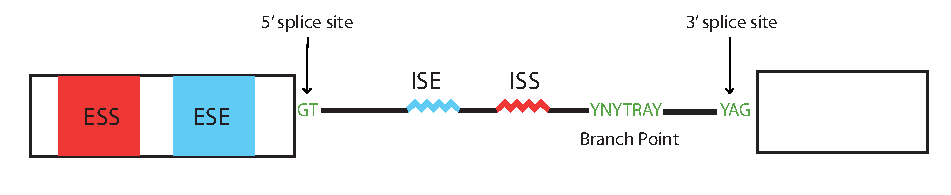
\includegraphics[width=\textwidth]{splicing_motifs}
    \caption[Cis-acting splicing motifs in eukaryotes]{Cis-acting splicing motifs in eukaryotes shown in an exon-intron-exon junction. The acceptor and donor dinucleotides are indicated at the 5' and 3' ends of the intron. ESE and ESS = exonic splicing enhancers and silencers. ISE and ISS = intron splicing enhancers and silencers. Y = pyrimidines.}
    \label{fig:splicing_motifs}   
  \end{figure}
AS is tightly regulated by several cis- and trans-acting factors. This tight regulation ensures splicing fidelity by correctly guiding the splicing machinery towards the target acceptor and donor splice sites, and by a complex interplay of splicing factors that promote and/or inhibit splicing (Figure \ref{fig:splicing_motifs}). Despite the apparent complexity of the splicing code \cite{Jaganathan2019-ah}, direct mutagenesis as well as computational approaches have elucidated several cis-acting sequence elements that guide the choice of splice sites and improve spliceosomal efficiency. These include exonic splicing enhancers (ESE), exonic splicing silencer (ESS), intronic splicing enhancers (ISE) and intronic splicing silencers (ISS). Splicing regulatory elements mostly work by recruiting various classes of trans-acting splicing factors to their target splicing sites. These factors either promote or hinder the recruitment of the spliceosomal complex. Most ESEs are bound by members of the serine/arginine rich proteins (SR proteins), which enhance the recruitment of several snRNPs necessary to initiate the splicing process (reviewed in \cite{Shepard2009-os}). The promotion of splicing is often countered by the recruitment of heterogenous nuclear ribonucleoproteins (hnRNPs) to ESS, which often block the recruitment of the splicing machinery \cite{Geuens2016-yz}. The disruption of this tight regulation underpins several diseases. Spinal muscular atrophy, a debilitating motor neuron disease, is caused by exon 7 skipping in \textit{SMN1}. Exon 7 skipping is caused by a single nucleotide substitution that alters the ESE sequence and results in a non-functional \textit{SMN1} protein isoform \cite{Monani1999-vf}.\\

\subsection{Cataloguing alternative splicing: progress and gaps}
Recent efforts to catalogue the human transcriptome have shown remarkable diversity of alternative isoforms. For example, the Reference Sequence (RefSeq) project uses a multi-modal approach to identify a high-confidence set of splice variants for each gene for thousands of organisms including over 770 mammalian transcriptomes \cite{OLeary2016-ci}. Manual curation by experts in addition to high-quality RNA-seq, proteomics, and histone marker datasets are used to build a bona fida set of gene splice variants. This effort has led to a 100-fold increase in the number of identified transcripts across mammalian species, from approximately 126,000 transcripts in 2003 to over 12 million transcripts in the latest RefSeq release (September 2023; \cite{refseq_ftp}). \\

Despite these significant advances, our knowledge of the distribution and roles of these splice variants in different tissues and cell types remains heavily underexplored. The evidence supporting the tissue-specificity of AS is contradictory. Wang et al. estimated that between 55-83\% of AS events vary between tissues in 15 studied human tissues and cell lines \cite{Wang2008-yg}. Others have shown that the majority of genes have a single dominant protein isoform in most tissues \cite{Ezkurdia2015-iv,Gonzalez-Porta2013-il}. However, many of these studies suffer from either biased transcriptomic or proteomic profiling methods or a small number of tissues. Fewer studies have attempted to systematically catalogue splice variants in an unbiased manner. In comparison, overall levels of gene expression in diverse tissues are being extensively studied by collaborative initiatives such as the Human Cell Atlas \cite{hca_resources}. Similar collaborative efforts that catalogue splice variants in an unbiased manner are warranted given the central role of AS in human health and disease.


\subsection{Technological limitations}
Several factors may explain why AS has received less attention compared to other transcriptional processes. The combinatorial nature of AS means that up to thousands of transcripts can be produced from the same genetic code. This poses several technological and analytical challenges. Most large-scale RNA-seq projects so far have relied on short-read sequencing to study the transcriptome. The complexity of AS patterns therefore makes it difficult to distinguish between distinct isoforms using 50-150 bp reads, as exonic sequences significantly overlap in alternative transcripts \cite{Lacroix2008-wq}. In principle, it is not possible to assign short reads to specific isoforms. \\

Creative technological and analytical techniques have been developed to assign short reads to their original transcript molecule. For example, Hagemann-Jensen et al. have recently applied a tagmentation strategy to map reads originating from the internal segments of gene bodies to UMI-tagged 5' reads. Using this technique, 30-50\% of reconstructed molecules were successfully assigned to a specific isoform \cite{Hagemann-Jensen2020-ob}. Additionally, computational techniques to reconstruct full isoforms from short reads have been developed. For example, Cufflinks relies on a reference transcriptome to estimate the most likely proportion of each splice variant given the observed RNA-seq reads \cite{Trapnell2012-zh}. Another method called rMATS estimates isoform proportions from the reads that support each type of AS event such as exon skipping and inclusion \cite{Shen2014-bq}. What these computational methods have in common is that they provide probabilistic estimates of isoform proportions, which underscores the inherent difficulty of obtaining a complete picture of isoform diversity from short-read RNA-seq experiments \cite{Shen2014-bq,Katz2010-kl}. These challenges explain why transcriptomic studies have focussed mostly on overall levels of gene expression, whose experimental and computational analysis workflow are more mature and suffer from less quantification uncertainty.

\subsection{Leafcutter as an intron-centric AS quantification method}
\begin{figure}
    \centering
    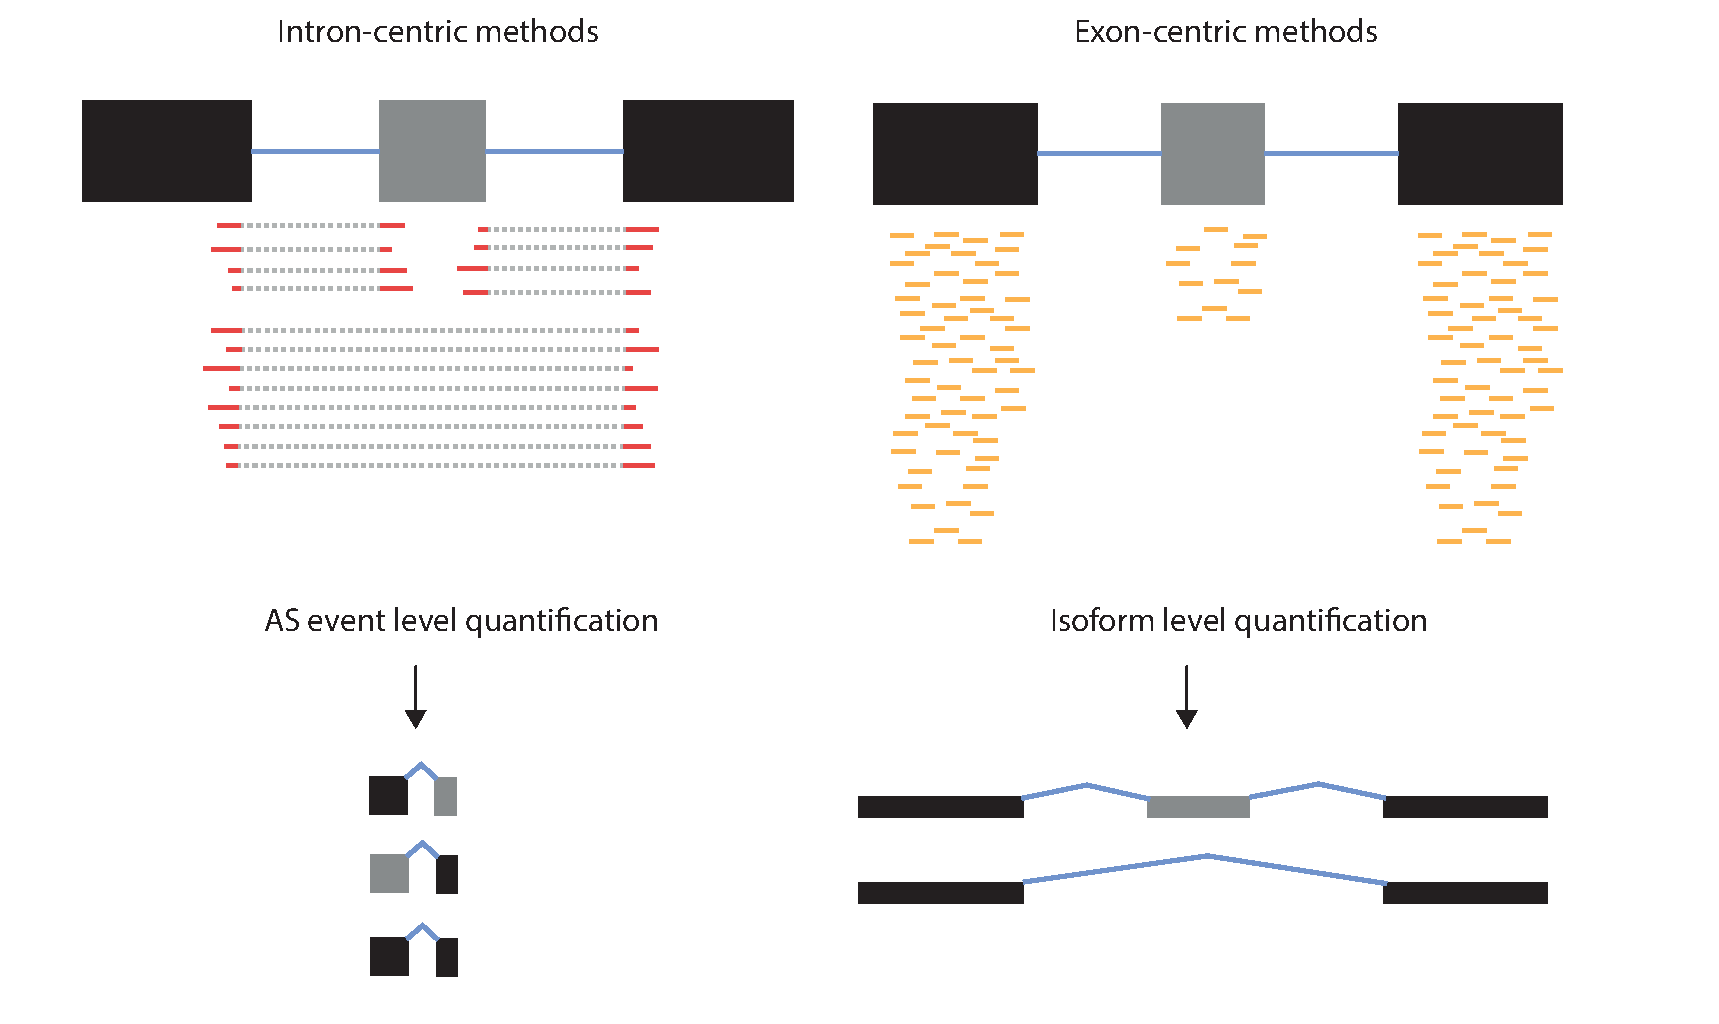
\includegraphics[width=\textwidth]{intron_exon_centric}
    \caption[Broad classification of alternative splicing quantification methods]{Alternative splicing quantification methods are broadly classified into exon-centric methods and intron-centric methods. Exon-centric methods use exonic RNA-seq reads to estimate isoform abundance. Intron-centric methods such as Leafcutter quantify individual alternative splicing events. }
    \label{fig:intron_exon_centric}   
  \end{figure}
AS quantification methods can be broadly divided into exon-centric and intron-centric methods. Exon-centric methods use exonic reads or a combination of exonic reads and reads that span two splice junctions (split reads) to infer isoform-level counts. These methods are heavily dependent on a known reference transcriptome, with some improvements to increase their ability to identify novel splice junctions \cite{Vaquero-Garcia2016-dv}. Their underlying assumption is that the relative abundance of exonic reads reflects the proportions of the unobserved isoforms. Conversely, intron-centric methods are based on the principle that AS proceeds in a step-wise fashion, where introns are excised from pre-mRNA. Instead of quantifying AS using exonic reads, intron-centric methods use observed split reads at each splice junction to directly quantify local AS events (Figure \ref{fig:intron_exon_centric}). The obvious advantage of intron-centric methods is that they provide less uncertain estimates of AS events as they do not attempt to provide probabilistic isoform-level quantifications. Moreover, they are able to detect novel splice junctions as they do not rely on a reference transcriptome to reconstruct isoforms. However, this comes at the cost of precision and interpretability. By definition, split reads that span exon-intron-exon junctions are less abundant than exonic reads. Consequently, intron-centric quantification methods such as Leafcutter build their AS quantification using many fewer reads than exon-centric methods such as MAJIQ, rMATS, or Cufflinks. Moreover, the interpretation of local AS events is usually less straightforward. Local AS events reflect local intron excision steps at each exon-intron-exon junction, but it is often unclear how different intron excision events relate to one another. \\

Leafcutter is an example of intron-centric AS quantification methods that use split reads to quantify local intron excision decisions. In its first pass, Leafcutter starts by pooling all observed split reads in all samples to identify a set of high-confidence intron excision events. In a second pass, Leafcutter counts per-sample the number of split reads that map to each intron identified in the first pass. To improve interpretability, Leafcutter then organises individual intron excision events into undirected graph structures called \textit{intron clusters}. Nodes represent local intron excision events which are connected by edges. The Leafcutter algorithm connects two nodes (i.e. introns) if they share a 5' or 3' splice site. The overall Leafcutter procedure results in functionally connected intron cluster where any two connected introns share an acceptor or donor splice site. Within each intron cluster, intron usage is then quantified as the proportion of all split reads that map to each individual intron. This final quantification is performed separately for each RNA-seq sample and the result is a matrix of intron usage ratio for all study samples. 



\subsection{Mapping sQTLs}

Given the complex regulatory network that underpins AS regulation, understanding the impact of genetic variation on AS patterns paves the pathway to understand the impact of AS dysregulation on human health. Moreover, understanding how AS patterns are regulated in relevant contexts can help us better understand the impact of disease-associate genetic variant on the transcriptome. Similar to expression QTLs, where genetic variants associated with gene abundance are mapped, AS quantifications can be used as a molecular trait to uncover the genetic determinant of AS (splicing QTLs; Figure \ref{fig:leafcutter_conceptual}).\\

\subsubsection{General outline of QTL mapping}
QTL mapping pipelines are relatively well-established. Typically, a QTL analysis pipeline starts by obtaining an adequate number of samples where a quantitative molecular phenotype of interest is assayed (e.g. gene expression). Initial quality control steps are applied to ensure that experimental issues such as sample mixups are addressed. For transcriptomic studies, the first step after initial QC is to align NGS short reads to a reference genome. To extract quantitative molecular features from aligned reads, a quantification method is applied. The quantification method of choice usually depends on the research question of interest. For example, overall levels of gene expression are quantified using methods that count all short reads that map to each gene, and provide a gene count matrix. Similarly, methods that quantify AS provide an isoform-level or AS-event-level quantification. At this stage, another round of QC is often needed to ensure that low-quality features are removed from subsequent QTL mapping steps. Again, this QC step depends on the molecular QTL of interest. For example, it is important to remove introns detected in a small number of individuals, as tiny individual variations in intron usage can result in spurious sQTL associations. \\

With a post-QC feature matrix, QTL mapping follows a number of standard steps. The most important step before QTL mapping is to ensure that the molecular feature is properly normalised. Normalisation ensures that features conform to the assumptions of a linear regression model: homoskedasticity and normal distribution. These two assumptions are not only prerequisites of linear regression, but also ensure that effect sizes can be interpreted apppropriately. First, heteroskedasticity occurs when the variance of the predicted variable (i.e. feature) is not equal for different values of the independent variable (i.e. different genotypes). Quantile normalisation is one of the most widely used approaches to ensure that a molecular feature has equal variance across all samples in a study, satisfying the homoskedasticity condition. Second, an inverse normal transformation is applied to each sample to ensure that the feature is normally distributed.\\ 

Each molecular QTL can be tested for association with genetic variants in \textit{cis} or in \textit{trans}. Typically, cis-QTL mapping tests the association between a molecular feature and all nearby variants (e.g. within a 1 mbp window), while trans-QTL mapping tests the association between a molecular feature and distant genetic variants (e.g. > 5mbp or on other chromosomes). Cis-QTL mapping is more common as it requires less statistical power to detect an association, owing to the much smaller set of tested variants. For each molecular feature, thousands of genetic variants are usually tested. Compared to GWASes where all variants are tested genome-wide, the number of tests performed in QTL mapping is highly dependent on each individual feature. Setting a significance threshold therefore requires a different approach to a traditional GWAS significance threshold. A common approach to correct for multiple testing is to perform a permutation test between genotypes and features. The genotype-feature mapping is permuted hundreds or even thousands of times and association tests are performed again, resulting in a null distribution of association statistics. The real association statistic is then compared to the null distribution to obtain an adjusted association statistic. This layer of multiple testing correction accounts for the thousands of variants tested for each molecular feature. Another layer of multiple testing correction is applied to account for the thousands of molecular features tested in the QTL study. \\

\subsubsection{Special considerations in sQTL mapping}
Although the steps outlined above are standard for all QTL studies, there are a few conceptual and methodological differences between splice and expression QTL mapping. Depending on the AS quantification method, the interpretation of sQTLs can vary. sQTLs discovered using isoform abundance as a molecular trait are the easiest to interpret. A significant isoform-level sQTL would be defined as a genetic variant that increases or decreases a particular transcript abundance. This interpretation is less straightforward when AS is quantified at the AS event level. When intron usage ratios are used as quantitative trait, a significant sQTL can be defined as a variant that changes the proportion of a particular intron within its intron cluster. Therefore, when sQTLs are mapped using intron usage ratios, it is often helpful to examine the effect of the discovered genetic variant on all neighbouring AS events to build a more complete picture of the splicing event under investigation. For example, in Figure \ref{fig:intron_exon_centric}, upon examination of all three AS events in the left-hand panel, it becomes clear that the identified AS events represents an exon inclusion/skipping event. Additionally, it is important to note that different AS events are often highly correlated. This is because intron usage ratios within an intron cluster always add up to 1. Therefore, a genetic variant that leads to increased usage of one intron also leads to decreased usage of one or more other introns. As a result, multiple significant sQTLs within a single intron cluster do not necessarily represent distinct regulatory effects, but rather highly correlated measurements. 
\begin{figure}[H]
    \centering
    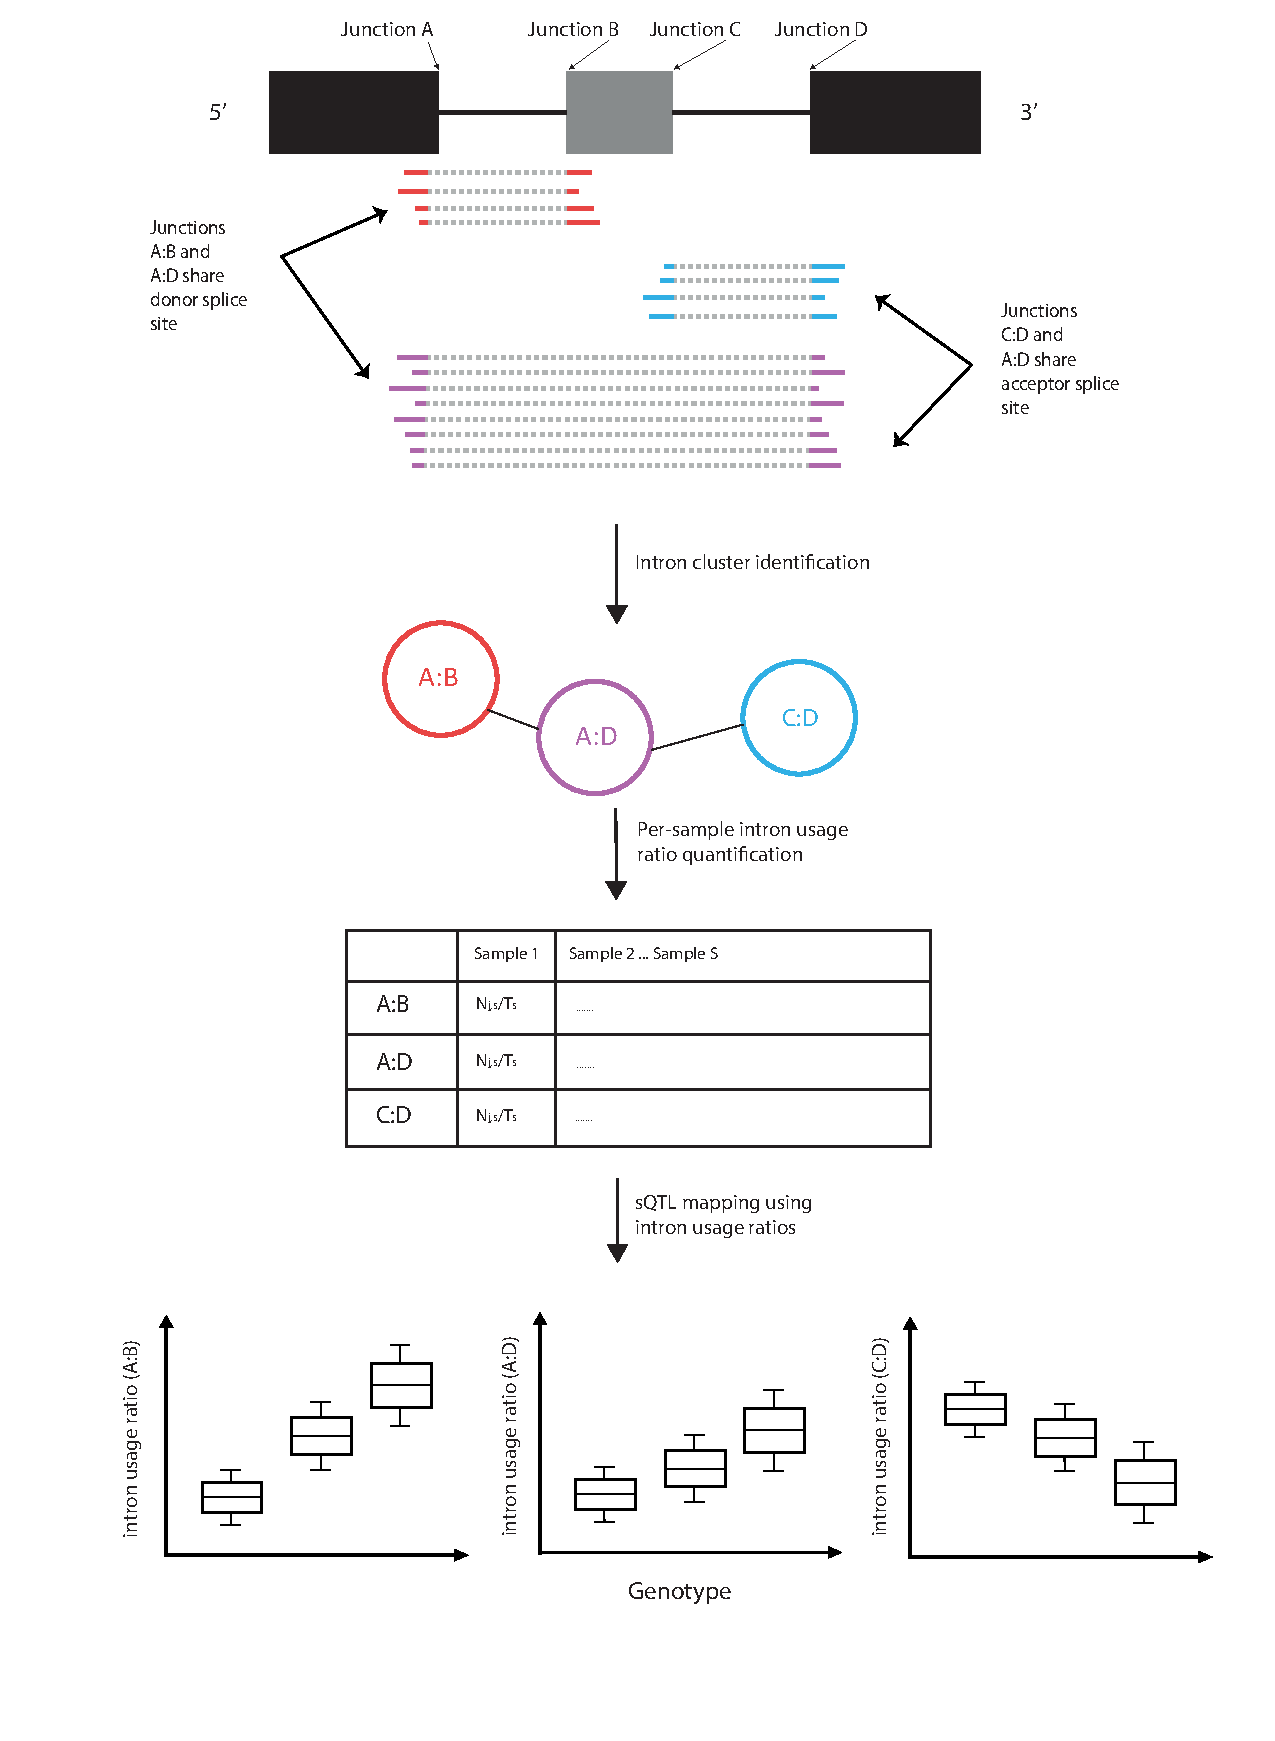
\includegraphics[width=\textwidth]{leafcutter_conceptual}
    \caption[Conceptual overview of splicing quantitative trait loci mapping using intron usage ratios]{Conceptual outline of sQTL mapping using intron usage ratios as quantitative traits. Intron clusters are identified from all pooled samples in a study. Quantification is then performed for each intron per sample. For a sample $S$, and an intron cluster with total number of reads $T_{S}$, the intron usage ratio for intron $j$ is defined as $\frac{N_{j,S}}{T_{S}}$. Intron usage ratios are then used as quantitative trait to map sQTLs in \textit{cis} with neighbouring genetic variants.}
    \label{fig:leafcutter_conceptual}   
  \end{figure}

\subsection{Comparing QTL effects in multiple contexts}
A long-standing question in QTL studies is how gene expression is genetically regulated in different tissues, cell types and environmental contexts. Answering this question is important to understand which transcriptomic effects of genetic variation are shared or distinct in different biological contexts. Context-dependence of QTL effects has often motivated multi-tissue QTL studies, with the assumption that profiling QTL effects in different contexts can draw a more complete picture of gene expression regulation. For example, in a comparison of eQTL effects between CD4+ T-cells and monocytes, Raj et al. \cite{Raj2014-xw} found that at least 42 genes had opposing eQTL effects in the two cell types. In line with this, Peters et al. \cite{Peters2016-zk} found that 87 genes had discordant eQTL effects in five different immune cell types. Although these dramatically discordant examples of genetic regulation represent a minority of QTL effects, the question of which QTL effects are modulated in a more subtle manner in different contexts remains relevant \cite{Fairfax2012-ur,Lee2014-zo,Umans2021-fv,Van_de_Geijn2020-zn,Gamazon2018-uz}.\\

Assessing the sharing of QTL effects in different treatment groups is non-trivial. In most QTL studies, QTL discovery is carried out separately for different treatment groups. This means that incomplete power may cause truly shared QTL effects to appear non-significant in some groups simply by chance. Direct comparison of statistical significance between different groups is therefore likely to overestimate the number of distinct QTL effects. To address this issue, several methods that probabilistically model effect sizes were developed \cite{Flutre2013-sp,Li2018-kr,Sul2013-xm, Urbut2019-gf}. Earlier methods were inspired by fixed-effects meta-analysis methods, and started from the assumption that any given eQTL effect is shared across all conditions and sought to find statistical evidence to the contrary (i.e. context-specificity).\\

Later, methods that learn the data-driven correlation structure were developed. For example, multivariate adaptive shrinkage (mash) empirically learns the patterns of effect sharing in the dataset under study, and allows for arbitrary patterns of sharing between different groups. For example, QTLs derived from different brain regions are expected to have highly correlated effect sizes. Usually, this correlation structure is learned from a random unbiased set of QTL effects (i.e. non-significant QTLs). A Bayesian approach is then applied to re-estimate effect sizes for a desired set of QTL effects (e.g. significant QTL effects). The posterior effect sizes are then tested for evidence of effect size heterogeneity between different groups, taking the underlying data-driven correlation structure into account. The obvious advantage of mash is that the re-estimated effect sizes take into account the empirical correlation structure in the dataset. However, this also means that significant QTL effects' sharing may be overestimated when the null QTL effects are highly correlated among the treatment groups. As a result, this may hide truly context-dependent QTL effects simply because there is not enough statistical evidence to suggest heterogeneity of effect sizes. Additionally, when significant QTL effects are tested for condition-specificity, only the lead QTL SNP is used. In many cases, sharing of the lead QTL SNP does not necessarily mean that the underlying causal variant is shared between different conditions. It has been previously shown that comparing the lead SNP between different association signals can lead to the false conclusion that the effects under comparison are shared \cite{Liu2019-fv}. A better approach should leverage the linkage disequilibrium structure to assess if two association signals under comparison are likely to be shared or distinct. Nonetheless, mash can still be useful if the degree of QTL sharing is interpreted as an upper bound, rather than an accurate estimate of QTL sharing.\\


\subsection{Linking disease-associated GWAS loci to QTLs}
In addition to understanding gene regulation, a major objective of QTL studies is to dissect the effects of disease-associated loci in relevant tissues and cell types. The simplest approach is to test the replication of the lead GWAS SNP in the QTL dataset. It is often compelling to assume that a replicated SNP may indicate that both gene expression and disease risk are driven by the same variant. In fact, lead SNP comparison was commonly used to implicate effector genes at many disease-associated loci. However, this direct SNP comparison was found to result in many false positives \cite{Liu2019-fv}. Therefore, more robust methods to compare pairs of association signals were developed to fill this gap. Particularly, statistical colocalisation methods take into account the association signal of all variants in a region to make a conclusion about a pair of association signals. Although the true causal variant may not be genotyped or imputed in either of the association studies, its effect is tagged by other variants in linkage disequilibrium with the true causal variant. Colocalisation methods leverages the linkage disequilibrium in a given locus to make an inference about two association signals. The underlying assumption is that if the two association signals are consistent across the region, it is likely that the same variant is driving both signals. Therefore, colocalisation results are only valid when the LD pattern is similar between the two association signals under comparison. This assumption only holds if the two association signals being compared are derived from populations with matching LD structures, an important consideration when colocalisng signals from GWAS and QTL studies. Additionally, standard colocalisation approaches only test the hypothesis that a \textit{single} shared variant underpins the two association signals. Many QTL studies have shown that secondary and even tertiary association signals have been discovered for several genes \cite{macromap-eqtl,De_Klein2023-ku}, and the same observation applies to GWAS signals. Violations of the single causal variant assumption at loci with multiple causal variants will result in decreased power to detect true colocalisations. Therefore, extensions to standard colocalisation identify independent association signal in each of the two cohorts, before proceeding to perform colocalisation analysis for each of the identified signals. This approach has been shown to increase the number of colocalised signals detected \cite{Wallace2021-rv}.\\  


\subsection{Current status of sQTL studies}
Several studies have investigated the genetic regulation of alternative splicing. These studies include relatively fewer multi-tissue or multi-cell-type studies as well as single-tissue or single-cell-type studies. Notably, virtually all of these studies are bulk RNA-seq studies because the most widely used single cell RNA-seq methods capture only a few bps at the start or end of each RNA molecule. The imminent development of single-cell long-read RNA-seq methods is set to change this by allowing full-length RNA isoforms to be directly mapped at a single-cell level \cite{Dong2023-xs}. Still, bulk sQTL studies have taught us a few interesting insights. In this section, I will focus on two relevant aspects of the genetic regulation of AS: context-specificity and role of AS in complex disease risk.\\

The most diverse sQTL study to date is the GTEx consortium, where eQTLs and sQTLs were mapped across 49 human tissues from 70-700 individuals. GTEx tissues represent a heterogenous mix of different cell types, which makes an investigation of cell-type-specificity of alternative splicing difficult. However, GTEx was still useful understand the patterns of alternative splicing sharing across tissues. It was found that tissue sharing follow a U-shaped distribution, meaning that the majority of sQTL effects were either found in a small number of tissues (1-5) or shared across almost all tissues (45-49 tissues). This pattern was less evident for eQTL effects, which suggested that sQTLs are generally more tissue-specific than eQTLs \cite{The_GTEx_Consortium2020-gg}. However, it is difficult to disentangle the effect of different statistical power in different tissues from true tissue specificity. Indeed, a subsequent re-analysis of the GTEx splicing data (Garrido-Martín et al. 2021 \cite{Garrido-Martin2021-sk}) found that sQTL effects with large effect sizes, which are more readily discovered with small sample sizes, tend to be shared between tissues, and vice versa. When Garrido-Martín et corrected for sample size differences between various tissues, they found that brain, testis, liver and skeletal muscles had large numbers of tissue-specific sQTLs. These observations show that sQTL effects, especially one with smaller effect sizes, show patterns of tissue-specificity. \\

sQTLs were also shown to contribute significantly to complex disease risk in two major meta-analysis of brain and immune cell sQTL studies. Qi et al. 2022 \cite{Qi2022-iz} mapped sQTLs from over 2800 RNA-seq samples, and discovered thousands of significant sQTLs and eQTLs. The availability of both eQTLs and sQTLs allowed them to compare their contribution to complex disease risk. To this end, they quantified the contribution of both sQTLs and eQTLs to the SNP heritability of 12 brain-related complex diseases, and showed that both molecular QTLs contributed roughly equally to disease heritability. Moreover, when they performed colocalisation with disease-associated loci, they found that both molecular QTLs implicated distinct gene sets. This finding was also mirrored in another eQTL and sQTL meta-analysis of 18 different immune cell types (Mu et al. 2021 \cite{Mu2021-ar}). Mu et al. compared the contribution of eQTLs sQTLs in different cell types to immune disease risk. Similar Qi et al., they also found a significant contribution of sQTLs, as measured by the number of loci that colocalised with high confidence with disease-associated loci. For many complex traits, this contribution often exceeded the contributionof eQTLs.\\

\subsection{Contribution of this thesis}
In the first part of my thesis, I will use iPSC-derived macrophages (MacroMap) to address the previously mentioned two aspects of alternative splicing regulation: the context specificity of AS regulation, and the contribution of AS to immune-mediated disease risk. Although the GTEx sQTL results indicate that AS regulation may be tissue specific, it does not provide an account of which genes are alternatively spliced in a cell-type or context-specific manner. This is mainly because GTEx tissues are a mixture of several cell types. Moreover, even fewer studies addressed the question of whether cells respond to environmental stimuli at the AS level. For example, do cells respond to pathogens by altering isoforms in genes relevant for microbial clearance? What role does the genetic regulation of AS play in such a response?\\

As part of the MacroMap project, iPSC-derived macrophages from over 200 individuals were exposed to a wide range of stimuli. I will describe how I used genotype and RNA-seq data to study the patterns of alternative splicing in different stimulation conditions, and to identify genetic variants that regulate alternative splicing in different macrophage environmental contexts. I will describe examples of the widespread differential splicing between stimulated and unstimulated macrophages, often implicating core innate immune response pathways. Additionally, I will show that alternative splicing regulation is often context-dependent, and that a considerable proportion of sQTL effects are modulated upon exposure to environmental stimuli. Finally, I will describe how I linked hundreds of immune disease loci to alternative splicing changes in macrophages and give examples of alternative splicing dysregylation by disease-associated risk loci. An important insight of this work is that in the context of IMD risk, the dysregulation of alternative splicing is at least as important as the dysregulation of overall levels of gene expression. Finally, I will highlight the potentially important role of lowly-used splice junctions in immune disease risk, a role that has been, so far, under-appreciated.

\section{Part II: sub-phenotype GWAS}
\subsection{Genome-wide association studies}
Complex disease risk is determined by a multitude of genetic and environmental factors. Over the last 18 years, genome-wide association studies (GWAS) have revolutionised our understanding of the genetic component of complex disease risk. The Wellcome Trust Case Control Consortium (WTCCC) ushered the era of GWAS studies by designing large-scale case-control cohorts for several common disorders. Since then, the case-control experimental design has been exploited in thousands of GWAS studies to uncover the genetic determinants of cardiovascular, metabolic, immune-mediated, musculoskeletal, neurological, and gastrointestinal diseases. In most cases, these cohorts are built through collaborative efforts between recruitment centres, hospitals and other healthcare facilities and research centers that identify disease cases and controls, and provide biological samples needed to conduct array-based or exome-based genotyping. The continuous growth of sample sizes has increased our ability to detect genome-wide significant loci associated with disease risk. These efforts have also revealed the extensively polygenic nature of most complex diseases, whereby hundreds of genetic loci increase or decrease disease risk with small effect sizes. The complexity of the genetic architecture of most common disease has initially made it more challenging to draw biological insights. Although most GWAS results were initially puzzling, over the last few years massive GWASes have revealed biological insights about common diseases \cite{Xue2018-ni,Aragam2022-ep}. This increased understanding was facilitated by the availability of functional genomic datasets as well as methodological advances in linking genetic variants to biological functions. 

\subsection{Inflammatory bowel disease}
\subsubsection{Epidemiology and classification}
Inflammatory bowel disease (IBD) encompasses a group of immune-mediated disorders of the gut. IBD poses a considerable burden for healthcare systems globally. In 2017, IBD affected over 6.8 million individuals worldwide, with a rising global burden since at least the 1990s. IBD incidence shows notable geographical variation, with the highest incidence reported in North America, the UK and northern Europe. Moreover, IBD incidence has notably risen in countries that are becoming increasingly "westernised" in terms of their environmental risk factors, such as China and South Korea, consistent with a significant environmental contribution to IBD \cite{Ng2013-of}.\\

IBD is broadly classified into two broad categories based on radiological, clinical and endoscopic features: ulcerative colitis (UC) and Crohn's disease (CD), although 6-13\% are classified as IBD unclassified (IBDU) \cite{Thurgate2019-xj}. The two classes show differences in terms of disease behaviour and location, clinical manifestations and prognosis. UC inflammation occurs in a continuous manner and is often characterised by chronic mucosal inflammation and leukocyte infiltration \cite{Hendrickson2002-ky}. UC usually starts near the rectum and diffuses proximally to different parts of the colon. On the other hand, CD can affect any part of the GI tract from mouth to anus and is characterised by patches of inflammation (skip areas). Inflammation often extends beyond the gut mucosa involving the submucosa. CD most frequently occurs in the ileo-coecal region followed by isolated terminal ileal inflammation. Clinically, CD is a heterogenous disease characterised by a remitting-relapsing clinical picture. Most patients experience abdominal pain, rectal bleeding, and altered bowel habits. However, other clinical aspects of CD vary between patients and can often make the difference between favourable or unfavourable disease course and prognosis. Some CD patients experience relatively infrequent CD flares, with milder symptoms that respond well to treatment. Others experience more frequent episodes of severe GI symptoms. Severe CD patients also often develop transmural manifestations such as penetrating disease, fistulas and abscess as well as extraintestinal manifestation involving the eye, joints and/or other systemic manifestations. Although the majority of CD patients undergo surgery at least once over their lifetime, patients who have non-penetrating non-fistulising CD manifestations are less likely to require surgery \cite{Lewis2010-gx}. %Understanding the genetic determinants of the different clinical aspects of CD is therefore crucial for a more nuanced biological insight into what drives disease course. 



\subsubsection{Risk factors of IBD}
IBD is a complex disease, which is likely caused by an interaction of genetic, environmental, and lifestyle factors. IBD has often been described as an "industrialised nations" diseases, with higher prevalence in developed countries. Epidemiological studies have shown increasing prevalence of IBD in nations that are becoming increasingly industrialised. Interestingly, second-generation immigrants from low-prevalence countries have experienced increasing incidence of IBD \cite{Bernstein2008-ln}. These observations have linked IBD risk to "industrialised" lifestyle factors, whereby environmental and lifestyle factors common in industrialised countries are thought to contribute to IBD risk. These changes have led to reduced exposure to infectious agents, improved hygiene and sanitation, an increasingly sedentary lifestyle and increased consumption of processed foods, and foods rich with sugar and saturated fats.\\

Smoking is the best described lifestyle factor linked to IBD risk. Smoking has been shown to increase risk of CD and decreasing risk of UC. However, the mechanism of this paradoxical association between smoking and IBD is not completely understood \cite{Richardson2003-pd}.  Other non-dietary factors include oral contraceptive pill intake, which was shown to increase both CD and UC risk \cite{Cornish2008-rn}, and appendectomy which was associated with reduced UC risk \cite{Koutroubakis2000-qt}.\\

The effect of lifestyle choices and diet on IBD have been extensively studied, but the results are often difficult to assess. Exercise is known to boost immunity and decrease proinflammatory cytokines. However, the severity of IBD symptoms often impacts patients' physical activity, and studies linking exercise to IBD progression have been therefore confounded by IBD severity \cite{Rozich2020-ui}. Similarly, alcohol and coffee consumption were not conclusively linked to IBD development or progression \cite{Yang2019-gt}. However, obesity has been shown to independently worsen IBD behaviour and increase likelihood of relapse \cite{Jain2019-oy}. Diet composition also plays an important role in IBD risk. Its role has been attributed to the effect of diet on the gut microbiota composition and bahaviour. For example, a Japanese study has shown a significant association between IBD risk and total fat and unsaturated fat intake, fish and shellfish consumption, and $\omega$-3 and $\omega$-6 fatty acids \cite{Reif1997-li}.\\



\subsection{Inflammatory bowel disease genetics}
The genetic component of IBD has been recognised for over 70 years via family studies on twins. Family studies have shown that monozygotic twins are more likely to co-inherit IBD compared to dizygotic twins, often with similar disease behaviour and location \cite{Ng2012-mf}. Over the last decade, several GWASes have identified over 240 loci associated with IBD susceptibility \cite{Jostins2012-ig,De_Lange2017-re,Liu2015-bx,Luo2017-kx}. The largest IBD GWAS studies have focussed on discovering both common and rare genetic variants associated with IBD susceptibility. These studies have revealed several key mechanistic insights regarding the pathogenesis of IBD including autophagy, host-microbe interactions, intestinal innate immune response, and impaired epithelial barrier function \cite{Khor2011-td,Jostins2012-ig}. These pathways seem to converge on a IBD pathogenesis model whereby impaired intestinal permeability, leads to microbial infiltration into the gut mucosa. This microbial incursion activates intra-epithelial cells to initiate a cascade of innate and adaptive immune responses aiming to limit microbial spreading and restore normal barrier function. The integration of hundreds of genetic loci with functional genomic datasets have clearly improved our understanding of IBD susceptibility. However, given the clinical heterogeneity of IBD sub-types, understanding the genetic determinants of their different clinical aspects is crucial for a more nuanced biological insight into what drives disease course.\\

% Fewer GWAS studies have dissected other clinical aspects of CD. 
% CD is a heterogenous subtype of IBD characterised by a remitting-relapsing clinical picture. Most patients experience abdominal pain, rectal bleeding, and altered bowel habits. However, other clinical aspects of CD vary between patients and can often make the difference between favourable or unfavourable disease course and prognosis. Some CD patients experience relatively infrequent CD flares, with milder symptoms that respond well to treatment. Others experience more frequent episodes of severe GI symptoms. Severe CD patients also often develop transmural manifestations such as penetrating disease, fistulas and abscess as well as extraintestinal manifestation involving the eye, joints and/or other systemic manifestations. Although the majority of CD patients undergo surgery at least once over their lifetime, patients who have non-penetrating non-fistulising CD manifestations are less likely to require surgery \cite{Lewis2010-gx}. Understanding the genetic determinants of the different clinical aspects of CD is therefore crucial for a more nuanced biological insight into what drives disease course.\\

\subsubsection{Growing interest in the genetic determinantsof disease sub-phenotypes}
The evident success of GWAS studies in improving our understanding of CD biology has sparked the interest in using them to dissect complex disease sub-phenotypes. However, disease sub-phenotype GWASes have generally lagged behind susceptibility GWASes, due to the difficulty of obtaining deep phenotypic or longitudinal data for similarly large cohorts. It has been previously suggested that the same genetic variants drive both disease susceptibility and disease sub-phenotypes. However, evidence in relatively smaller sub-phenotype GWASes suggests that the genetic variants that underpin disease susceptibility and disease sub-phenotypes may also be distinct \cite{Iwaki2019-mf,Severe_Covid-19_GWAS_Group2020-rn}. Both paradigms raise interesting questions about the genetic architecture of disease susceptibility and sub-phenotypes. Under the former paradigm, it will be particularly important to understand the relationship between the effect of each variant on susceptibility and sub-phenotype risks. For example, for a given variant associated with both disease sub-phenotype and susceptibility, is the susceptibility risk truly driven by sub-phenotype risk? As sub-phenotype GWASes become more commonplace, it will be particularly interesting to compare the effects sizes of each variant on both susceptibility and disease sub-phenotypes. This may lead to better stratification of disease risk based on distinct sub-phenotype risk profiles. Under the latter paradigm, it is important to understand which distinct biological pathways are involved in disease sub-phenotypes risk and how they interact with disease susceptibility pathways. For example, fistulising CD has been hypothesised to originate as an epithelial-to-mesenchymal transformation, whereby stationary epithelial cells gain migratory features. Is this transformation accelerated by the impaired intestinal barrier and subsequent immune activation that likely underpins CD susceptibility?\\

The genetic architecture of CD sub-phenotypes has been explored in a number of studies. Longitudinal and deep phenotypic data from CD cohorts of thousands of patients were used alongside genetic data to map genetic variants associated with disease location, behaviour, surgery and prognosis. Because these studies are considerably less powered than susceptibility GWASes, they have only given an initial glimpse into the genetic architecture of CD sub-phenotypes. Therefore, it is still not possible to draw a conclusive answer to the question whether or not CD susceptibility and sub-phenotypes share genetic underpinnings. In the rest of this section, I will focus on two studies by Cleynen et al. 2016 \cite{Cleynen2016-ha} and Lee et al. 2017 \cite{Lee2017-tl} as notable examples of CD sub-phenotype GWASes. \\

Cleynen et al. \cite{Cleynen2016-ha} used 11 years of longitudinal data from approximately 17,000 CD patients to study the genetic determinants of CD sub-phenotypes. They performed several within-case GWASes of CD age-at-diagnosis, location, behaviour and surgery. Across all their CD analyses, they found three genome-wide significant loci at \textit{MST1} and \textit{NOD2} as well as an MHC association. Both the MHC and  \textit{NOD2} loci were associated with ileal versus colonic disease and with a penetrating (B3) versus inflammatory or stricturing disease (B1 or B2). Despite the small number of genome-wide significant loci, the authors built IBD polygenic risk score to compare individuals with different disease locations and behaviours. The main insight from their work was the rejection of the binary classification of IBD into CD and UC. Based on a polygenic risk score (PRS) comparison between individuals with different disease locations, they proposed a novel classification which places ileo-colonic CD as an intermediate form between ileal CD and UC. \\

Based on the discovered loci, the genetic relationship between CD susceptibility and CD sub-phenotypes is difficult to assess. For example, the \textit{NOD2} lead variant (rs2066847) is a frameshift variant that has been previously associated with CD susceptibility in several studies \cite{Barrett2008-lg,Jostins2012-ig} (P-value=$6\times10^{-209}$ in Jostins et al. data). However, the lead MHC variant (rs6930777) was not genome-wide significant in any CD susceptibility GWAS (source: GWAS catalogue accessed in November 2023). \\

% \begin{table}[]
%   \caption{Genome-wide significant loci associated with CD behaviour (B1 versus B2/B3) and CD location (ileal versus colonic) from Cleynen et al. 2021. CD susceptibility associations were obtained from the GWAS catalogue accessed in November 2023. N/A means no CD susceptibility association was available because none passed the minimum P-value threshold. N/R means association statistic was not reported.}
%   \label{tab:cleynen_gws}
%   \begin{tabular}{|l|l|l|l|l|l|l|l|}
%   \hline
%   SNP       & CD behavior P-value  & CD behaviour OR  & CD location P-value  & CD location OR   & CD susceptibility P-value & CD suscptibility OR & CD susceptibility study \\ \hline
%   rs6930777 & $2\times10^{-3}$     & 0.89 (0.82-0.96) & $8.13\times10^{-23}$ & 0.58 (0.52-0.65) & N/A                       & N/A                 & N/A                     \\ \hline
%   rs2066847 & $5.73\times10^{-10}$ & 1.31 (1.21-1.42) & $1.01\times10^{-35}$ & 2.50 (2.14-2.92) & $6 \times10^{-209}$       & N/R                 & Jostins et al.          \\ \hline
%   \end{tabular}
%   \end{table}
Comparatively, Cleynen et al. had a much smaller sample size than many CD susceptibility GWASes. The growth of sub-phenotype GWASes' sample sizes will enable a more systematic comparison of genome-wide significant associations of CD susceptibility and sub-phenotype variants. However, their PRS comparison may give a clue that may contribute to answering this question. The PRSs they built to compare different IBD forms were based on lead variants from all known IBD susceptibility loci. The ability of these PRSs to distinguish "macroscopic" features of IBD (e.g. CD versus UC or ileal versus colonic CD) lends support to the hypothesis that the genetic architectures of susceptibility and location are not entirely distinct. It is worth noting that the differences in PRS distribution between these groupings were quite small, but this could also be attributed to the low predictive power of PRSs in general.\\

A later study by Lee et al. \cite{Lee2017-tl} showed that the genetic determinants of CD prognosis were largely distinct from CD susceptibility variants. Lee et al. performed a within-case GWAS between two CD subpopulations at opposite ends of the prognosis spectrum. Poor prognosis individuals were defined as patients who experienced frequent CD flares that did not respond to treatment with immunomodulators and/or surgery. Good prognosis patients were defined as CD patients who showed good long-term response to treatment. Their analysis found four genome-wide significant loci in \textit{FOXO3} and \textit{XACT}, an intergenic locus in \textit{IGFBP1}-\textit{IGFBP3}, as well as an MHC association. These association were not found to be associated with CD susceptibility in any previous CD GWAS studies. Additionally, the authors found no evidence of genome-wide genetic correlation between CD susceptibility and CD prognosis, although it has to be noted that CD prognosis GWAS may have been underpowered to detect a significant genetic correlation ($r_{g}=-0.51$; P-value=0.12). Unlike Cleynen et al., these lines of evidence support the alternate hypothesis that the genetic architectures of CD susceptibility and CD prognosis, an example of a CD sub-phenotype, are distinct. Interestingly, a recent GWAS of multiple sclerosis progression reported a similar observation. The authors compared the long-term cognitive outcomes of MS patients with the highest and lowest MS PRSs, and found that PRSs did not differentiate between individuals with poor versus good MS prognosis \cite{ms_susceptibility}. Similarly, a GWAS of epilepsy prognosis concluded that it is unlikely that epilepsy susceptibility variants affect epilepsy prognosis \cite{Speed2014-lz}.\\

At this stage of CD sub-phenotype GWASes, it is perhaps too early to answer the question conclusively, since very little is known about the biological mechanisms behind each CD sub-phenotype. This is set to change as large-scale IBD resources grow and enable well-powered sub-phenotype GWASes that give us a better understanding of the biology behind each CD sub-phenotype. \\


\subsection{Contribution of this thesis to sub-phenotype understanding}
In my thesis, I attempt to identify the genetic variants associated with perianal CD, as an example of a CD sub-phenotype. pCD is a severe CD sub-phenotype characterised by abscess and fistula formation around the anal region. Collaborative efforts have enabled detailed clinical phenotyping of thousands of CD patients, including information on perianal symptoms. I describe a GWAS meta-analysis between CD patients with and without pCD in two IBD patient cohorts (UK IBD Genetics Consortium and IBD BioResource). As a follow-up, I also studied the genetics of sporadic perianal manifestations in the general population. Although perianal symptoms are highly enriched among CD patients, perianal fistulising disease also occurs sporadically, often not accompanied by CD. To understand the genetics of the two types of perianal manifestations, I performed an additional GWAS meta-analysis between individuals who report sporadic perianal disease and healthy controls in the UK Biobank and FinnGen. This meta-analysis revealed several genome-wide significant loci associated with sporadic perianal manifestations. My initial assessment shows that none of these loci replicate in the pCD meta-analysis, possibly suggesting distinct mechanisms driving both types of perianal manifestations. Overall, the aim of chapters 3 and 4 of my thesis is to study perianal manifestations as an example of a CD sub-phenotype, both in the context of CD and in its sporadic forms in the general population. 





% Moreover, investigating the interaction of these factors with the immune system has led to the "hygiene hypothesis".  

% \subsubsection{Colocalisation}

% \subsubsection{Other approaches}

% % Statistical modelling of effect sizes tests the alternative hypothesis that a given effect size is significantly different in one or more treatment groups. Different methods test this hypothesis in different ways. Earlier methods were inspired by fixed-effects meta-analysis approaches and 
% % The complex regulatory network of cis-acting elements and trans-acting factors suggests that regulatory errors can arise 

% % Since the 1970s, alternative splicing (AS) has emerged as an important post-transcriptional modification. AS has been shown to remarkably increase the coding potential of an otherwise fixed repertoire of genes. Through diversification of the transcriptome, AS contributes to phenotypic complexity in higher organisms. Previous work has shown that AS is more prevalent in higher eukaryotes compared to lower eukaryotes, and in vertebrates compared to invertebrates (10.1038/nrg2776). Our appreciation of the role of AS has also changed over time. Today, we know that 95% of multi-exonic genes are alternatively spliced, compared to an estimate of only 5-35% shortly after the Human Genome Project (https://www.hindawi.com/journals/ijeb/2012/596274/; https://www.ncbi.nlm.nih.gov/pmc/articles/PMC2443848/). 


% \subsection{why we need qtl studies}
% \subsection{why molecular qtls are context dependent - same dna - different gene expression}
% \subsection{why is it important to understand disease-associated variants in a relevant context}
% \subsection{the variety of molecular QTLs: caQTLs, histone marker QTLs..etc}
% \subsection{Most studies have focussed on overall levels of gene expression}
% %!TEX root = ../thesis.tex
%*******************************************************************************
%****************************** Second Chapter *********************************
%*******************************************************************************

\chapter{Genetic regulation of alternative splicing in iPSC-derived macrophages}

\ifpdf
    \graphicspath{{Chapter2/Figs/Raster/}{Chapter2/Figs/PDF/}{Chapter2/Figs/}}
\else
    \graphicspath{{Chapter2/Figs/Vector/}{Chapter2/Figs/}}
\fi
\tracingcommands=1
\section{Contributions}
Dr Nikolaos I Panousis has provided expression QTL colocalisation results that were compared to my own splicing QTL colocalisation results, and eQTL summary statistics that were colocalisaed with my own sQTL summary statistics. All other analyses described here are the result of my work. This work is currently under review in the journal \textit{Nature Communications} and a preprint is available online \cite{macromap-sqtl}.

\section{Introduction}
Genome wide association studies (GWAS) have uncovered thousands of genetic loci associated with susceptibility to immune-mediated diseases (IMD). Over 90\% of these loci are located in non-coding regions of the genome \cite{Maurano2012-yw}, making it difficult to gain insights into causal disease biology. These non-coding disease-associated loci are enriched in gene regulatory regions, and are therefore thought to modulate gene expression \cite{Schaub2012-cy}. Expression quantitative trait loci (eQTL) mapping has been widely used to characterise the downstream effects of genetic variants on gene expression \cite{Vosa2021-pb,The_GTEx_Consortium2020-gg}. Despite the increasing number of available eQTL datasets \cite{Kerimov2021-gh}, IMD-associated loci have remained largely unexplained by existing QTL maps. For example, Chun et al. 2017 (ref: \cite{Chun2017-uz}) found that only 25\% of IMD-associated loci colocalised with eQTLs from three immune cell types. \\

Multiple explanations have been put forward to justify the incomplete overlap between GWAS loci and existing eQTL maps, including a need for more diverse molecular QTL maps across disease-relevant cell types and environmental conditions. Moreover, it has recently been suggested that common variants driving complex diseases and gene expression are systematically different, and that alternative molecular QTLs (such as those affecting splicing, chromatin accessibility and chromatin interactions) may be more likely to colocalise with disease associated loci \cite{Mostafavi2022-tg}. Unfortunately, most QTL mapping studies have focussed on associating genetic variation with overall levels of gene expression without considering, for example, variation in transcript isoforms. The few studies that have mapped genetic variants associated with alternative splicing (splicing quantitative trait loci or sQTLs) have shown their promise for understanding disease \cite{Li2016-wu,Kim-Hellmuth2020-gz}. There is thus an urgent need for sQTL maps to be constructed across a broad range of environmental contexts for disease relevant cell types. \\

In this chapter, I mapped sQTLs in iPSC-derived macrophages in 12 different cellular conditions obtained from 209 individuals at two timepoints after stimulation. I quantify the extent to which alternative splicing responds to macrophage stimulation, and how sQTLs and response sQTLs (re-sQTLs) are shared across environmental contexts. I also explore the contribution of alternative splicing and sQTLs to IMD risk. Finally, I contextualise these findings within an ongoing scientific debate about the functional and evolutionary relevance of low-usage splicing events and discuss the implications of this work on the design of future transcriptomics studies. \\
\section{Methods}

\subsection{Differentiation of Induced Pluripotent Stem Cell Lines (iPSC) Into Macrophages}

iPSCs obtained from healthy donors of European descent were selected from the HipSci Consortium \cite{Kilpinen2017-qm}, and were differentiated to macrophages using a previously published protocol \cite{Alasoo2018-pv}. Of 315 lines initially selected, 227 (71.6\%) were successfully differentiated. RNA-seq libraries were produced for 217, which represented 209 lines after quality control. Differentiated macrophages have been shown to be transcriptionally similar to monocyte-derived macrophages \cite{Alasoo2018-pv}. The differentiated naive macrophages were then stimulated with a diverse panel of adjuvants, resulting in 10 stimulation conditions, as well as naive differentiated (Ctrl\_6 and Ctrl\_24) and undifferentiated controls (Prec\_D0 and Prec\_D2). mRNA was harvested 6 and 24 hours after stimulation. Multiple cell lines were derived from a varying number of individuals in each stimulation condition (ranging between 177-202 individuals), resulting in a total of 4,698 unique RNA-seq libraries across all conditions. Detailed experimental protocol for this study is provided by Panousis et al. 2023 \cite{macromap-eqtl}.

\subsection{Genotype Imputation and Quality Control}
Individuals who donated cell lines were previously genotyped through the HipSci project \cite{Kilpinen2017-qm}. Genotypes were obtained for each cell line from the HipSci Consortium  (hipsci.org) and genotype calling and imputation to  UK10K and 1000 Genomes Phase I is described in \cite{Kilpinen2017-qm}. CrossMap \cite{Zhao2014-ve} was used to lift over from GRCh37 to GRCh38. Imputed variants with a low imputation score (INFO < 0.4), Hardy-Weinberg equilibrium P-value < $10^{-6}$, a minor allele frequency (MAF) < 0.05 or a missingness rate > 0.001 were filtered out. For the remaining variants, genotype principal components (PCs) were calculated using EIGENSTRAT \cite{Price2006-kr} to correct for population stratification.

\subsection{RNA-seq Quality Control And Read Mapping}
RNA-seq reads (FASTQ files) were mapped to the reference genome build GRCh38 using splice-aware aligner STAR v2.6.1 \cite{Dobin2013-hs} using the following parameters: 

\begin{verbatim}
--twopassMode Basic --outSAMstrandField intronMotif
--outSAMtype BAM SortedByCoordinate --outSAMunmapped Within
--outSAMattributes All --outFilterMismatchNoverReadLmax 0.04
--outSAMmultNmax 1 --limitBAMsortRAM 40000000000
--sjdbOverhang 74 --waspOutputMode SAMtag
\end{verbatim}
The parameter \Verb_sjdbOverhang_ is particularly relevant as it sets the minimum number of basepairs each split read has to map to on either side of the splice junction. I used a a value of 74 as it is recommended to be set to $read length -1$. Finally, this step outputs BAM files that I used for the identification of split reads using LeafCutter. \Verb_outSAMstrandField_ outputs the strand to which each read was mapped to. This is an important check when splice junctions are linked to genes to ensure that the identified splice junction and gene are transcribed from the same strand. 

\subsection{WASP filtering of ambiguously-mapped reads}
It has been shown that ambiguously-mapped reads (RNA-seq reads that map to multiple genomic positions) can bias the number of split reads mapped across splice junctions \cite{Van_de_Geijn2015-lb}. Genetic variants that overlap with splice junctions can potentially introduce unnoticed mapping ambiguity when an alternative allele increases mapping ambiguity. It is particularly important to guard against this when mapping sQTLs, since decreased splice junction can indicate a mapping ambiguity effect of an alternative allele rather than a true genetic effect.

WASP \cite{Van_de_Geijn2015-lb} identifies an ambiguously-mapped read by replacing the reference allele in each genomic location that harbours a genetic variant with the alternative alleles and then repeats read mapping. Reads whose mapping ambiguity increases after allele replacement are flagged (\Verb_vW_=2-7). In the previous step, I used STAR with the parameter \Verb_waspOutputMode_, which flags reads that pass the WASP filter with \Verb_[vW]=1_.  I therefore only removed read alignments which did not have tag \Verb_[vW]=1_ using this command in SAMtools \cite{Li2009-yk}:

\begin{verbatim}
samtools view -S -b -e 
"[vW]!=2 && [vW]!=3 && [vW]!=4 && [vW]!=5 && [vW]!=6 && [vW]!=7"
\end{verbatim}

\subsection{Identification of split reads}
I identified split reads from BAM files from the previous step using \Verb_regtools_ \cite{Cotto2023-yp} which outputs the number of split reads supporting each intron as \Verb_.junc_ files. I used the following command and parameters:
\begin{verbatim}regtools junctions extract -s 0 -a 8 -m 50 -M 500000 \end{verbatim}
These parameters specify the minimum and maximum intron length (50 bp and 500,000 bps in length, respectively), and a minimum splice junction anchor length of 8 bps. The last parameter means that there must be reads supporting at least 8 basepairs at either side of an intron. 

\subsection{Intron clustering using LeafCutter}
Mapped split reads (as \Verb_.junc_ files) were used to perform intron clustering using the LeafCutter script \Verb+leafcutter_cluster.py+:

\begin{verbatim}
python leafcutter_cluster_regtools_py3.py -j .junc -m 50 -l 500000
\end{verbatim}
A minimum number of 50 split reads across samples was required to support an intron cluster. Maximum intron length used was 500 kbp. 
For each identified intron cluster with introns $1…j$, LeafCutter quantifies intron usage ratio R for intron $k$ as:
$$R_{k}=\frac{X_k}{ \sum_{i=1}^{j}X_{i} }$$
where $X_k$ is the number of split reads that belong to an identified intron $k$. A conceptual outline of the intron clustering process is provided in the thesis Introduction and in Figure \ref{fig:leafcutter_conceptual}.

\subsection{Differential splicing analysis}
I performed differential splicing analysis between each of the 10 stimulated conditions and their corresponding timepoint controls (e.g. sLPS\_6 vs Ctrl\_6 and sLPS\_24 vs Ctrl\_24). LeafCutter differential splicing analysis tool (script \Verb+leafcutter_ds.R+) \cite{Li2018-ll} was used with eight experimental covariates: run ID, donor, library preparation method, sex, differentiation media, purity, estimated cell diameter, and differentiation time, and with  the following parameters:
\begin{verbatim}
–min-samples-per-intron 50 –min-samples-per-group 50 –min-coverage 30
\end{verbatim}
This ensures that for a splice junction to be considered differentially spliced, it must be supported by at least 50 RNA-seq samples per condition, and 30 split reads in total. This ensures the robustness of the differential splicing analysis and avoids false positives due to technical differences in splice junction calls between conditions.

\subsection{UMAP clustering}
I performed the UMAP clustering on normalised intron usage ratios for introns that that were detected across all 24 conditions. This ensures that clustering is not based on introns that are not detected in a one or a small number of condition. I performed UMAP clustering after 3 pre-processing steps. First, I performed quantile normalisation on raw intron usage ratios using the R function \Verb+normalize.quantiles()+. Second, I performed rank-based inverse normal transformation using the R function \Verb+rbint()+. Third, I regressed out eight technical covariates similar to the ones included in the differential splicing analysis: run ID, Donor, library preparation method, sex, differentiation media, purity, estimated cell diameter, and differentiation time. I used the \Verb+umap+ R package to perform UMAP clustering \cite{McInnes2018-fe} (github.com/tkonopka/umap). 

\subsection{Intron usage ratio quality control and normalization}
\label{sec:intron_qc_methods}
%In order to use intron usage as a quantitative trait, I first used the LeafCutter script \linebreak \Verb+prepare_phenotype_table.py+, which applies two default filters at the intron level. It removes introns which have an intron usage ratio=0 in more than 40\% of samples, and those with a standard deviation $< 5\times10^{-3}$ (Figure \ref{fig:qc_introns_num}). The script also applies quantile normalization to the introns which ensures that different samples follow the same intron usage ratio distribution. 
Because LeafCutter performs annotation-free quantification of intron usage, the output introns are not assigned to specific genes. One way to assign introns to genes is to map the 5' and 3' ends of each identified intron to known exon-intron junctions in an annotation database such as GENCODE. However, this will result in novel introns not being assigned to any gene since their 5' and/or 3' ends will not map to any known exon-intron junction. To overcome this issue, I mapped intron clusters, rather than individual introns, to known exon-intron junctions in GENCODE v27. Specifically, an intron cluster will be assigned to a specific gene if \textit{any} intron within the intron cluster maps to a known exon-intron junction within the gene. After this procedure, intron clusters with no gene assignment were removed from the sQTL analysis. 

\begin{figure}[H]
  \centering
  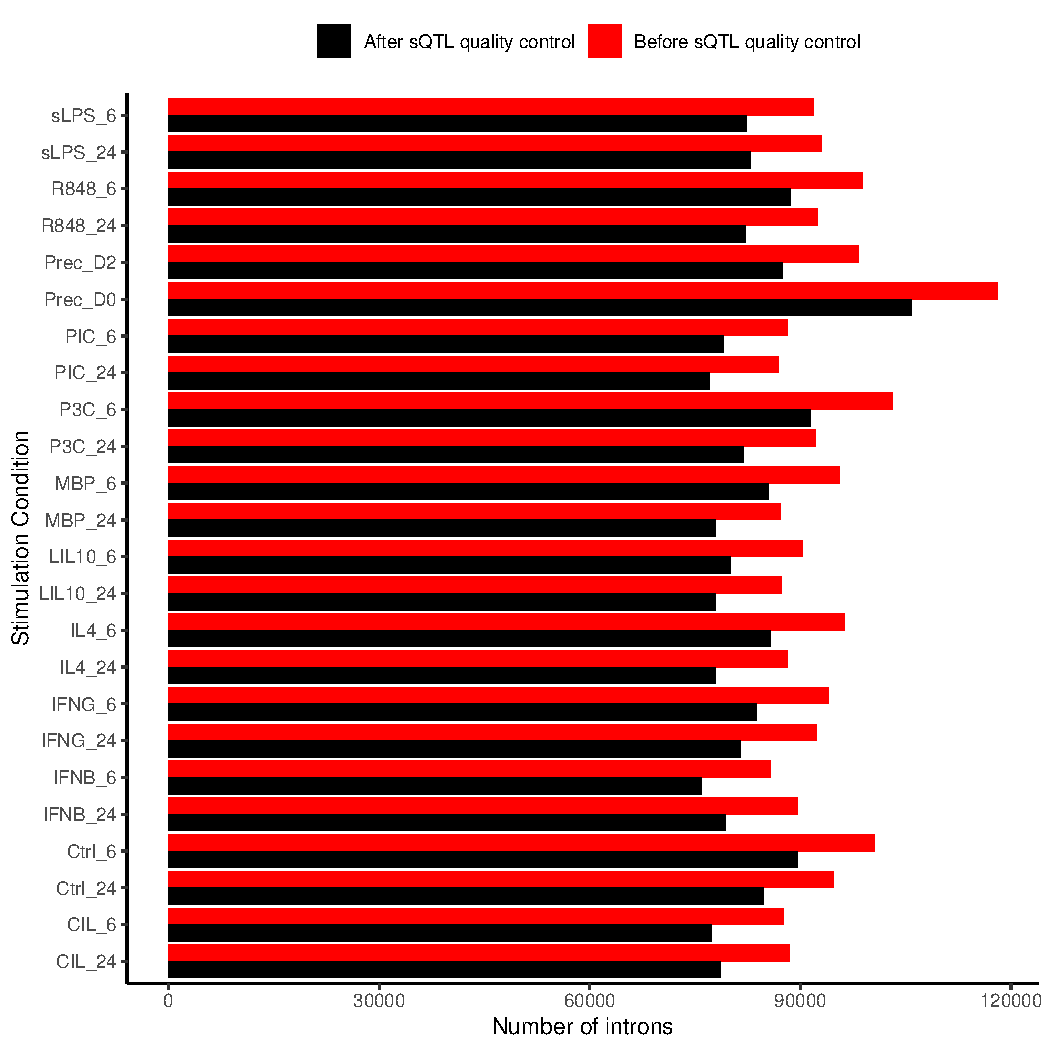
\includegraphics[width=0.7\textwidth]{qc_introns_num}
  \caption[Number of introns before and after intron quality control]{Number of introns identified in the intron clustering procedure of
  LeafCutter (before intron sQTL quality control; in red) and the number of introns that were
  used as input to map sQTLs (after intron sQTL quality control; in black).}
  \label{fig:qc_introns_num}   
\end{figure}

% To understand which alternative splicing events were affected by genetic variation, I mapped splicing QTLs using intron usage ratios as a quantitative trait. The quantification of intron usage ratios was performed separately for each stimulation condition, and the sQTL pipeline was therefore run for each condition separately. 
To minimise the risk of false positive sQTLs, I removed quantified splice junctions that may cause spurious associations when sQTLs are mapped across individuals. These spurious associations can be driven by splice junctions supported by a small number of samples. Therefore, I removed intron clusters that have non-zero usage ratios in more than 40\% of samples. I also removed introns with low variance across samples (standard deviation < 0.005). Additionally, in order to make all introns follow the same distribution and to ensure the interpretability of resulting effect sizes, I applied quantile normalisation to intron usage ratios. %Quantile normalised ratios were then subjected to a rank-based inverse normal transformation in order to ensure that they follow a normal distribution. 
\subsection{Mapping sQTLs using intron usage ratios}
I mapped sQTLs using normalised intron usage ratios and genotype data from samples within each condition separately. Variants in a 1 mega base pair (mbp) window around the transcription start site (TSS) were tested for association with intron usage ratios. Genotype-intron association was modelled using a linear regression model implemented in QTLtools \cite{Delaneau2017-dg} with the parameters:
\begin{verbatim}
--permute 1000 --window 1000000 --grp-best --normal
\end{verbatim}
The \Verb+--normal+ option ensures that intron usage ratios follow a normal distribution by applying a rank-based inverse normal transformation. The option \Verb+-grep-best+ allows phenotypes (intron usage ratios) to be grouped. Within each phenotype group, the genotype-phenotype sample labels are permuted in exactly the same way. This allows P-values for phenotypes within the same group to be compared with each other and for QTLtools to report the best associated phenotype per group. I grouped introns by the gene they belong to, and report the best associated variant-intron per gene. \\

In all of my subsequent analyses, I included the first three genotypic principal components (PC) as covariates. In order to remove unwanted variability in intron usage ratios, I mapped sQTLs separately in different conditions using 0, 1, 2, 3, 4, 5, 6, 7, 8, 9, 10, 20 and 50  intron usage ratio PCs as additional covariates. I then counted the number of genes with significant sQTL effects (sGene) at a false discovery rate (FDR) $\leq$ 0.05 using the R package \Verb+qvalue+ v2.16.0 \cite{Storey2003-zd}. In all my downstream analyses, I use the number of intron usage ratio PCs that maximises the number of sGenes discovered (Figure \ref{fig:num_sgenes_PCs})

\begin{figure}[H]
  \centering
  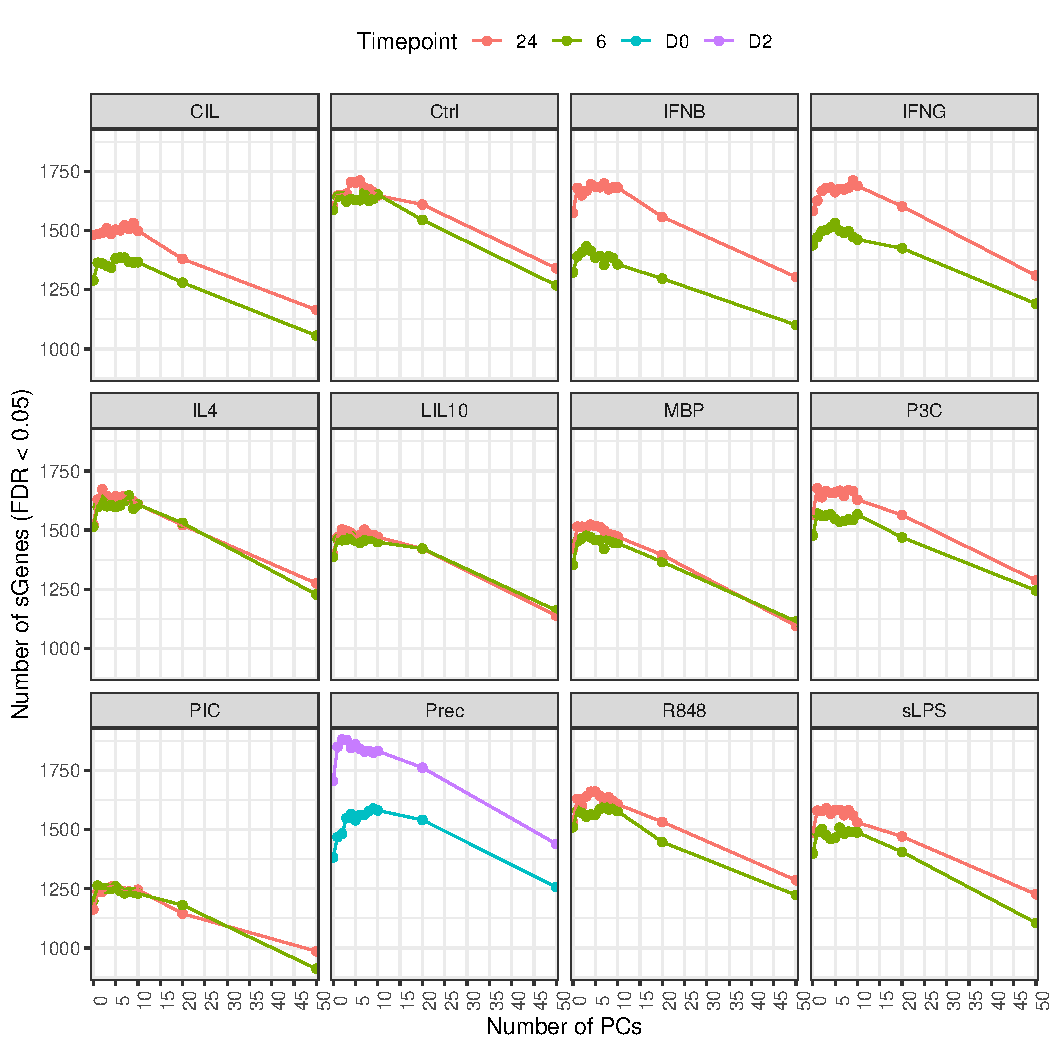
\includegraphics[width=0.7\textwidth]{num_sgenes_PCs}
  \caption[Number of principal components used in sQTL mapping and number of discovered sGenes]{Number of intron usage ratio principal components used as
  covariates (x-axis) versus the number of genes for which a significant sQTL effect was found
  (y-axis) coloured by time point (6=6 hours, 24=24 hours, D0=Day 0, D2=Day 2).}
  \label{fig:num_sgenes_PCs}   
\end{figure}




\subsection{Condition-specificity analysis using mash}
\label{sec:mash_methods}
I tested the condition-specificity of sQTLs using the R package \Verb+mashR+ v0.2.57 \cite{Urbut2019-gf}. mashR is an adaptive shrinkage framework that can be used to compare effect size estimates in a multi-tissue or multi-condition association study. It outputs re-estimated effect size estimates in addition to a statistic indicating if effect sizes between two conditions are significantly different from each other (local false sign rate; LFSR). I used this framework to test if a given sQTL effect is a "response sQTL", meaning that its effect size is significantly different in a stimulated macrophage condition from unstimulated macrophages. mashR requires training data to learn the correlation structure in the data from a set of canonical and data-driven covariance matrices (i.e. adaptive). To achieve this, mashR requires a randomly sampled set of QTL associations to learn the mixture components of a diverse set of covariance matrices. I used $10^6$ randomly sampled sQTL associations as the random training subset (effect sizes and standard errors). Mash can also be trained using a baseline condition, against which re-estimated effect sizes are compared (I used Ctrl\_24 as a baseline condition). The learned model can be used to re-estimate "posterior" summary statistics for any desired set of sQTL associations by providing their effect sizes and standard errors. In my analysis, I recomputed effect sizes and LFSR for two sets of sQTL effects: 
\begin{enumerate}
\item Lead SNP for significant sQTLs (FDR < 0.05) per sGene within each stimulated condition. I used this to estimate the number of sGenes with at least one response sQTL (Figure \ref{fig:sqtl}b).
\item Lead SNP for colocalised genes (PP4 $\geq$ 0.75) in the condition in which the colocalisation was detected. I used this to estimate the proportion of colocalised genes with a response sQTL within each stimulated condition (Figure \ref{fig:coloc_cum_response_sqtl}). 
\end{enumerate}
\subsection{Genome-wide summary statistics preprocessing}
GWAS summary statistics used for the colocalisation analysis were downloaded from either the GWAS catalogue \cite{Buniello2019-wb} or from UK BioBank GWAS summary statistics (\cite{Zhou2018-jh}; Table \ref{tab:gws_studies}). Summary statistics were formatted using a custom script so that each file contains at least: the chromosome and position (GRCh38) of each associated variant, effect size, and standard error. 

\begin{table}

  \caption[GWAS studies used in the colocalisation analysis with MacroMap QTLs]{\label{tab:gws_studies}GWAS studies used in the colocalisation analysis. Study accession for GWAS summary statistics downloaded from the GWAS catalogue are shown. Phenotype IDs for the UK Biobank summary statistics are also shown (obtained from https://pheweb.org/UKB-SAIGE/pheno/). PMID = PubMed ID. }
  \centering
  \begin{tabular}[t]{|>{\raggedright\arraybackslash}p{6em}|>{\raggedright\arraybackslash}p{6em}|>{\raggedright\arraybackslash}p{6em}|>{\raggedleft\arraybackslash}p{6em}|>{\raggedright\arraybackslash}p{6em}|}
  \hline
  Trait & Journal & Publication Date & PMID & Study Accession\\
  \hline
  Atopic dermatitis & Nat Genet & 19/10/2015 & 26482879 & GCST003184\\
  \hline
  Allergic asthma & Nat Genet & 21/05/2018 & 29785011 & GCST007563\\
  \hline
  Allergy & Nat Genet & 30/10/2017 & 29083406 & GCST005038\\
  \hline
  Ankylosing spondylitis & Nat Genet & 01/07/2013 & 23749187 & GCST005529\\
  \hline
  Asthma & Nat Commun & 15/04/2020 & 32296059 & GCST010043\\
  \hline
  Childhood onset asthma & Am J Hum Genet & 28/03/2019 & 30929738 & GCST007800\\
  \hline
  Crohn's disease & Nat Genet & 09/01/2017 & 28067908 & GCST004132\\
  \hline
  Celiac disease & Nat Genet & 06/11/2011 & 22057235 & GCST005523\\
  \hline
  Diverticulosis and diverticulitis & UK BIOBANK & 24/10/2018 & 30104761 & 562\\
  \hline
  Fasciitis & UK BIOBANK & 24/10/2018 & 30104761 & 728.7\\
  \hline
  Multiple sclerosis & Nat Genet & 01/11/2013 & 24076602 & GCST005531\\
  \hline
  Osteoarthritis & Nat Genet & 21/01/2019 & 30664745 & GCST007093\\
  \hline
  Osteoarthrosis & UK BIOBANK & 24/10/2018 & & 740\\
  \hline
  Contracture of palmar fascia & UK BIOBANK & 24/10/2018 & 30104761 & 728.71\\
  \hline
  Primary biliary cirrhosis & Nat Genet & 01/10/2012 & 22961000 & GCST005581\\
  \hline
  Psoriasis & Nat Genet & 01/12/2012 & 23143594 & GCST005527\\
  \hline
  Rheumatoid arthritis & Nature & 25/12/2013 & 24390342 & GCST002318\\
  \hline
  Primary sclerosing cholangitis & Nat Genet & 19/12/2016 & 27992413 & GCST004030\\
  \hline
  Systemic lupus erythematosus & Nat Commun & 17/07/2017 & 28714469 & GCST007400\\
  \hline
  Systemic sclerosis & Nat Commun & 31/10/2019 & 31672989 & GCST009131\\
  \hline
  Ulcerative colitis & Nat Genet & 09/01/2017 & 28067908 & GCST004133\\
  \hline
  \end{tabular}
  \end{table}

\subsection{Identification of genome-wide significant loci from IMD GWAS summary statistics and colocalisation analysis}
To define genome-wide significant loci, I identified all variants that passed the genome-wide significance P-value threshold $< 5\times10^{-8}$ in each downloaded GWAS summary statistics file. I ordered these SNPs from the lowest to the highest P-value and then iterated over each of them. At each iteration, I defined a 1 Mbp window centred around the SNP. If a SNP falls within a locus that has been defined in a previous iteration, it is not used to define a new locus. 

% For each genome-wide significant locus, I first identified the set of all genes whose TSS falls within the locus. I then performed pairwise colocalisation tests for all the intron usage ratios (within each of these genes) and the GWAS association signal. I performed these colocalisation tests within each of the 24 conditions. I matched variants between the sQTL and GWAS association signals by position on GRCh38 only since not all GWAS studies provided the effect alleles. I performed colocalisation analysis using the R package coloc v5.1.131 and I discarded GWAS-intron pairs that have < 2 variants in common. Only SNPs in common between each GWAS study and MacroMap's genotypic data are considered. This procedure output a list of tested introns per GWAS per condition. The same procedure was used for GTEx sQTLs. Locus plots for the colocalisation were produced using the locuscomparer R package \cite{Liu2019-fv}. Heatmaps for visualising PP4 values were generated using the ComplexHeatmap R packages \cite{Gu2016-oc}.

\subsection{Colocalisation analysis}
In order to link the IMD genome-wide significant loci identified in the previous step to effector genes, I performed statistical colocalisation between IMD-associated loci and sQTLs from all MacroMap conditions. Colocalisation analysis is a statistical approach that uses summary statistics from two association studies in order to make an inference about whether the two association signals are likely to be driven by a shared causal variant. In this regard, five different hypothesis regarding the relationship between the two association signals are tested:
\begin{itemize}
  \item $H_{0}$: none of the two signals are associated with their corresponding traits
  \item $H_{1}$: only the first signal is associated with its corresponding trait
  \item $H_{2}$: only the second signal is associated with it corresponding trait
  \item $H_{3}$: the two signals are associated with their corresponding traits, with different underlying genetic variants
  \item $H_{4}$: the two signals are associated with their corresponding traits, and share a single underlying genetic variant.
\end{itemize}
Certainty about each of these hypotheses is quantified as a posterior probability. Therefore, colocalisation analysis outputs five different posterior probabilities: $PP_{0}$, $PP_{1}$, $PP_{2}$, $PP_{3}$, and $PP_{4}$. Statistical colocalisation is implemented in the R package \Verb+coloc v5.1.2+.\\

% To maximise the ability of \Verb+coloc+ to identify effector genes, I downloaded summary statistics from GTEx v8, a large compendium of expression and splicing quantitative trait loci (eQTLs and sQTLs) mapped from RNA-seq samples obtained from 49 human tissues, ranging in sample sizes from 73-706 individuals. eQTLs and sQTLs were mapped in a 1mbp window centred around the transcript start site (TSS) of each gene (cis-eQTLs and cis-sQTLs) using genotyped or imputed variants with MAF $\geq$ 0.01.

Within each genome-wide significant locus, I identified a list of splice junctions to be tested. To achieve this, for each locus I defined a 1 mbp window around the index variant at each locus, and created a set of splice junctions whose respective gene TSS is located within this window. Next, I performed colocalisation analysis between the IMD summary statistics and each sQTLs summary statistics for each gene in the window. I used the \Verb+coloc.abf()+ function, which takes as input effect sizes and standard errors of each variant from the IMD  and sQTL being tested. Importantly, \Verb+coloc.abf()+ does not require the effect sizes to be aligned to the same effect allele, as the Bayes Factor calculation implemented in \Verb+coloc+ relies on the $Z^{2}$ statistic to compute the posterior probabilities. Finally, I used the default priors implemented in \Verb+coloc.abf()+: prior probability a SNP is associated with IMD=$10^{-4}$, prior probability a SNP is associated with sQTL=$10^{-4}$.
\subsection{Colocalisation between significant sQTLs and eQTLs}
I performed statistical colocalisation between all significant sQTLs (FDR < 0.05) and eQTLs from the same genes to investigate whether the sQTL and eQTL signals within sGenes are likely to be driven by the same causal variant. I only colocalised the intron with the highest association P-value per sGene using the same approach described in the previous section.
\newpage
\section{Results}

\subsection{MacroMap: a resource for studying macrophage transcriptome}

Induced pluripotent stem cell lines (iPSC) from 209 healthy unrelated individuals, generated as part of the HipSci project \cite{Kilpinen2017-qm}, were differentiated into iPSC-derived macrophages (experimental protocol described in Panousis et al. 2023 \cite{macromap-eqtl}). RNA was harvested from macrophage precursors at day 0 (Prec\_D0) and day 2 (Prec\_D2).
Naïve macrophages were exposed to a panel of 10 stimuli, and RNA was obtained and processed 6 and 24 hours after stimulation (in addition to unstimulated controls; Ctrl\_6 and Ctrl\_24), resulting in a total of 24 different conditions. I quantified alternative splicing from split reads (reads mapping across two splice junctions) using LeafCutter, which quantifies alternative splicing as intron usage ratios \cite{Li2018-ll}. I derived an intron usage ratio matrix for each of the 24 conditions and used this for differential splicing analysis and sQTL mapping.\\

\begin{figure}[H]
  \centering
  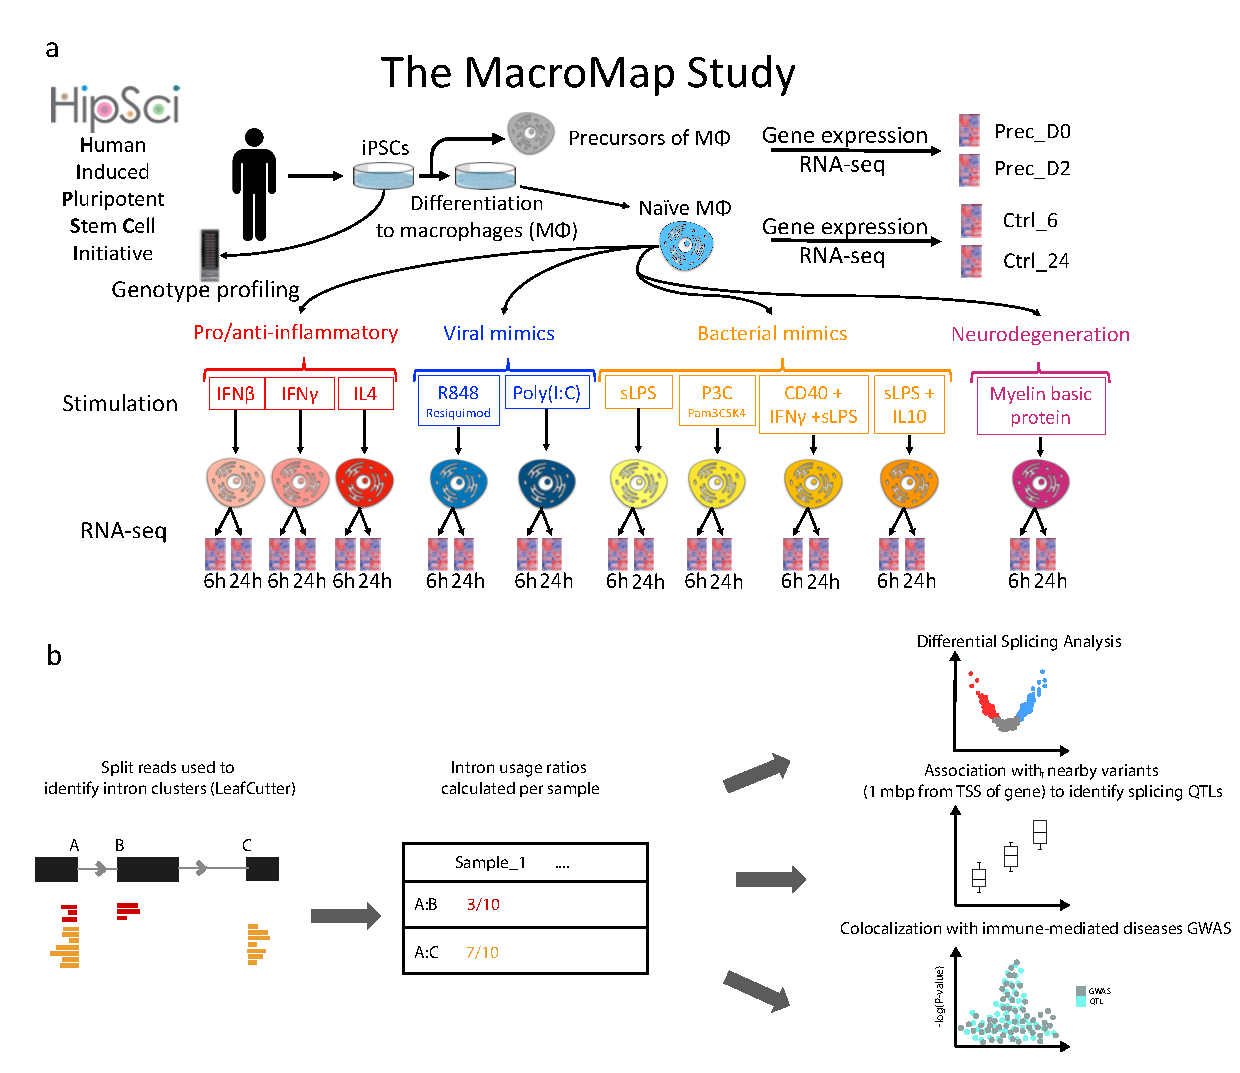
\includegraphics[width=\textwidth]{study_desc}
  \caption[MacroMap study overview]{Overview of study: (a) Genotyped iPSC cell lines were differentiated into macrophages, and RNA was harvested before differentiation (Prec\_D0) and 2 days after starting differentiation (Prec\_D2). RNA was also harvested from differentiated macrophages at 6 and 24 hours (Ctrl\_6 and Ctrl\_24). Naive macrophages were then exposed to a panel of 10 stimuli and RNA was harvested at 6 and 24 hours after stimulation. (b) Split reads were used to quantify intron usage ratios on an individual level using LeafCutter. Split reads were then used for differential splicing analysis between naive and stimulated conditions, and as a quantitative trait to map splicing quantitative trait loci (sQTLs). sQTLs were then colocalised with 21 immune-mediated disease GWAS summary statistics.}
  \label{fig:study_desc}   
\end{figure}


\subsection{Alternative splicing patterns during the macrophage differentiation process}
In order to visualise general patterns of intron usage across conditions, I projected intron usage ratios in all samples on a UMAP. Since intron usage QC was performed separately for different conditions, not all introns were shared across conditions. Therefore, I created the UMAP projection using only the introns that passed QC in all conditions (N=40,044).\\

Overall, I found that macrophage precursors (Prec\_D0) clustered separately from all other conditions. Moreover, precursors at day 2 (Prec\_D2) clustered together with naïve macrophages, suggesting that splicing changes start early during the seven-day macrophage differentiation process (Figure \ref{fig:ds}a). I also observed a clear separation between stimulated cells harvested after 6 and 24 hours, a separation that I did not observe between unstimulated macrophages (Ctrl\_6 and Ctrl\_24; Figure \ref{fig:ds}b). These observations show that splicing changes are observed both during iPSC differentiation into macrophages and following macrophage stimulation. \\



\begin{figure}[H]
  \centering
  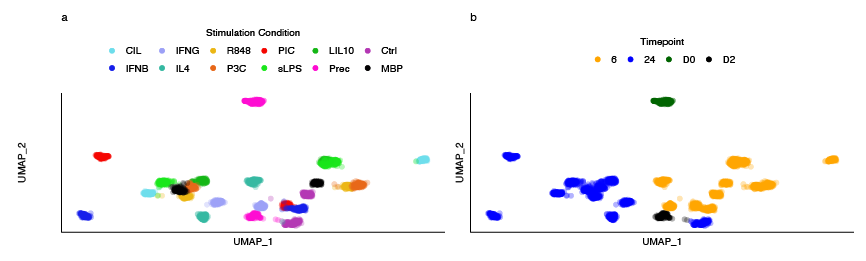
\includegraphics[width=\textwidth]{Vector/umap.png}
  \caption[UMAP of intron usage ratios in different stimulation conditions and timepoints]{ UMAP of intron usage ratios in different stimulation conditions, coloured both by (a) different stimulation conditions and (b) by time point.}
  \label{fig:umap}   
\end{figure}
Although UMAPs are useful to visualise general patterns in the data, they are less useful to make inferences about the correlation structure due to the non-linear nature of a UMAP transformation. Therefore, I confirmed these patterns by measuring the correlation between different conditions. Since a large proportion of introns show low variability across samples, which may inflate correlation estimates, I only used the top 20,000 variable introns. In confirmation of the UMAP patterns, Prec\_D0 showed relatively weaker correlation with both differentiated macrophages at day 2 (Pearson correlation coefficient $\rho$ with Prec\_D2=0.84) and the two differentiated control conditions ($\rho$=0.85 and 0.84 with Ctrl\_6 and Ctrl\_24). Conversely, correlation between Prec\_D2 and both Ctrl\_6 and Ctrl\_24 was stronger ($\rho$=0.94 and 0.95, respectively), confirming the trends observed in the UMAP. This difference in correlation strength was even more striking when I used the top 10,000 and top 5,000 variable introns, showing that it is not an artefact of the number of variable introns used to measure correlations between these conditions.\\

\begin{figure}[H]
  \centering
  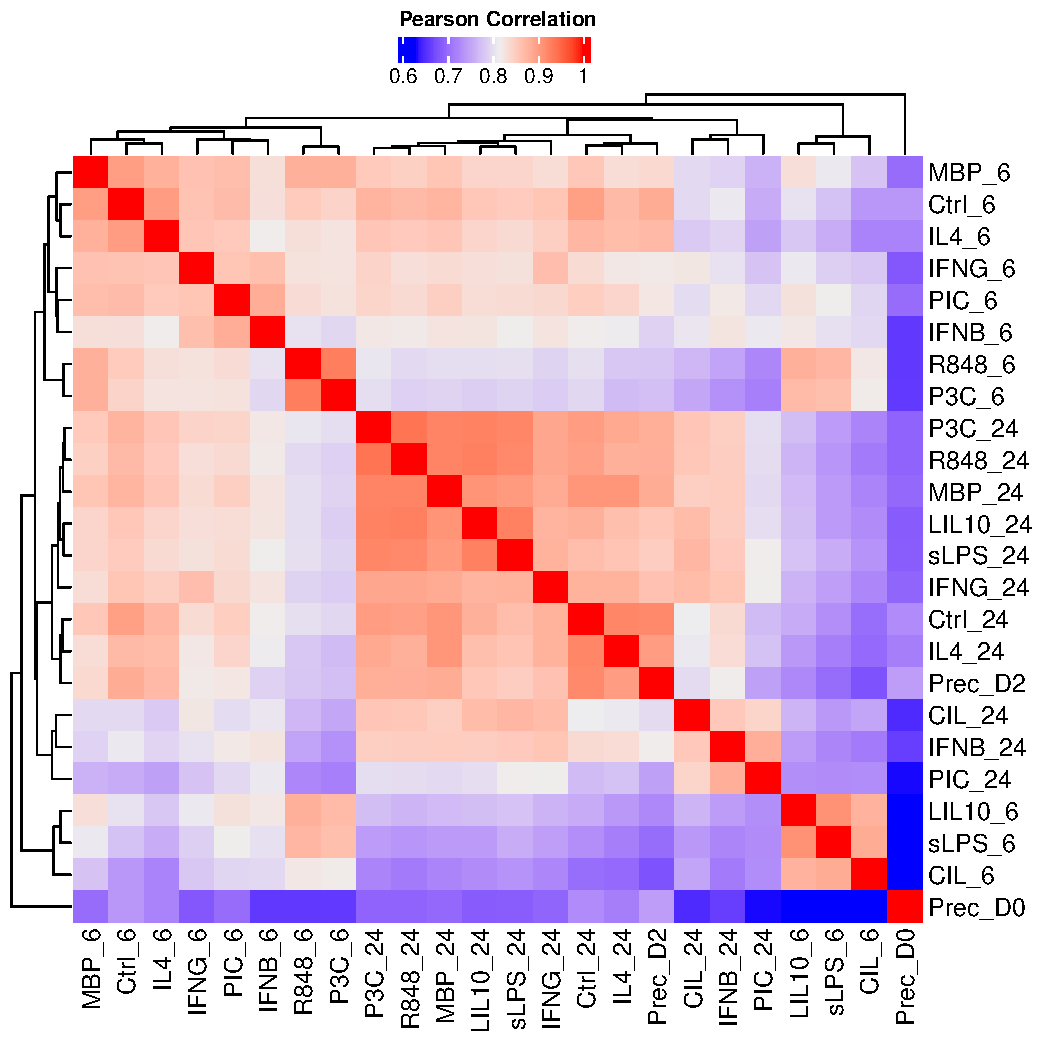
\includegraphics[width=0.7\textwidth]{cond_corr}
  \caption[Correlation heatmap of intron usage ratios]{Heatmap showing Pearson correlation coefficient values between all 24 conditions. Usage ratios of the top 20,000 variable introns (highest variance across all conditions) were $log_{10}$ transformed and the mean usage was calculated across samples within each condition. Pairwise correlation coefficients were then calculated between the means of log transformed ratios.}
  \label{fig:cond_corr}   
\end{figure}

\subsection{Macrophage response genes are differentially spliced upon stimulation}
In order to formally quantify how many genes are alternatively spliced upon stimulation, I performed differential splicing analysis (DSA) between naïve and stimulated macrophages. The DSA method implemented in LeafCutter jointly quantifies the overall changes at the level of intron clusters, which are groupings of introns that share an acceptor and/or donor splice site. In total, I found that 3,464 genes were alternatively spliced upon stimulation (adjusted P-value < 0.05 and |log effect size| > 0.5). Notably, stimulation with IL4 had the least effect on splicing (110 and 94 genes in macrophages harvested after 6 and 24 hours, respectively; Figure \ref{fig:ds}), corroborating previous reports where stimulation with IL4 did not cause dramatic changes to the splicing patterns of macrophages \cite{Liu2018-fh}. \\

The large number of differentially spliced genes motivated me to understand which biological pathways are subjected to differential splicing upon macrophage stimulation. In particular, I wanted to investigate whether macrophages respond to pathogens by activating splicing programmes in genes that are import to eliminate pathogens and initiate an immune response. In this section, I will summarise the enriched REACTOME pathways in two representative stimulation conditions. These two conditions were chosen to represent two broad classes of stimuli used in the MacroMap experimental design: Lipopolysaccharides as an example of bacterial stimulation and PolyI:C as a representative of viral stimulation.\\




\begin{figure}[H]
  \centering
  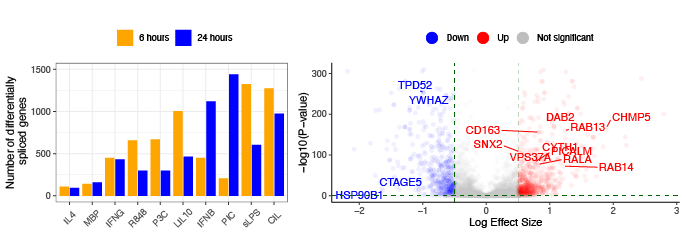
\includegraphics[width=\textwidth]{Vector/ds.png}
  \caption[Number of differentially spliced genes and volcano plot of differentially spliced genes in sLPS\_6]{(Left) Number of differentially spliced genes between naive and stimulated macrophages after 6 hours (yellow) and 24 hours (blue) (Right) Volcano plot showing differentially spliced genes 6 hours after sLPS stimulation, with log effect size on the x-axis (for each gene the intron with the largest absolute effect size is shown) and -log10 of adjusted P-value on the y-axis. Colours indicate the direction of intron usage change (blue indicating reduced usage and red indicating greater usage in stimulated cells versus naive cells). Some genes that belong to the "vesicle-mediated transport" REACTOME pathway are indicated.}
  \label{fig:ds}   
\end{figure}
Stimulation with LPS led to the differential splicing of genes in the cytokine signalling pathway (84 genes; P-value=$9.1\times10^{-8}$), the vesicle-mediated transport pathway (68 genes; P-value=$10^{-6}$), and the class I MHC mediated antigen processing and presentation pathway (47 genes; P-value=$7.95\times10^{-6}$; Figure \ref{fig:ds_sLPS_6_vs_Ctrl_6}). Within genes that belong to the vesicle-mediated transport pathway, several genes that code for members of the RAB protein family were differentially spliced upon stimulation (including \textit{RAB1B, RAB4A, RAB9A, RAB11A, RAB13, RAB14} and \textit{RABEPK}; Figure \ref{fig:ds}). RAB proteins are GTPases that coordinate membrane trafficking by regulating the formation, movement and fusion of vesicles with their destination membrane \cite{Stenmark2009-ju}. For example, I observed greater usage of the first exon of a non-canonical transcript of \textit{RAB13} (\textit{RAB13-205}), and lower usage of the canonical first exon (\textit{RAB13-201}; difference in percentage spliced in ($\Delta$PSI)=0.046 and -0.05, respectively). The alternative usage of the first exon may also be reflected at the level of protein products as the two annotated transcripts that start with these two alternative first exons have different amino acids sequences (203 and 122 amino acids respectively). Although this finding suggests that stimulation with LPS leads to an alternative \textit{RAB13} isoforms being expressed by macrophages, little is known about the particular functions of these isoforms. \textit{RAB13} has been previously shown to coordinate the formation of actin filaments through which vesicles are transported across the cell \cite{Sakane2012-km}, but the functional characterisation of the different isoforms of \textit{RAB13} are still lacking.\\

\begin{figure}[H]
  \centering
  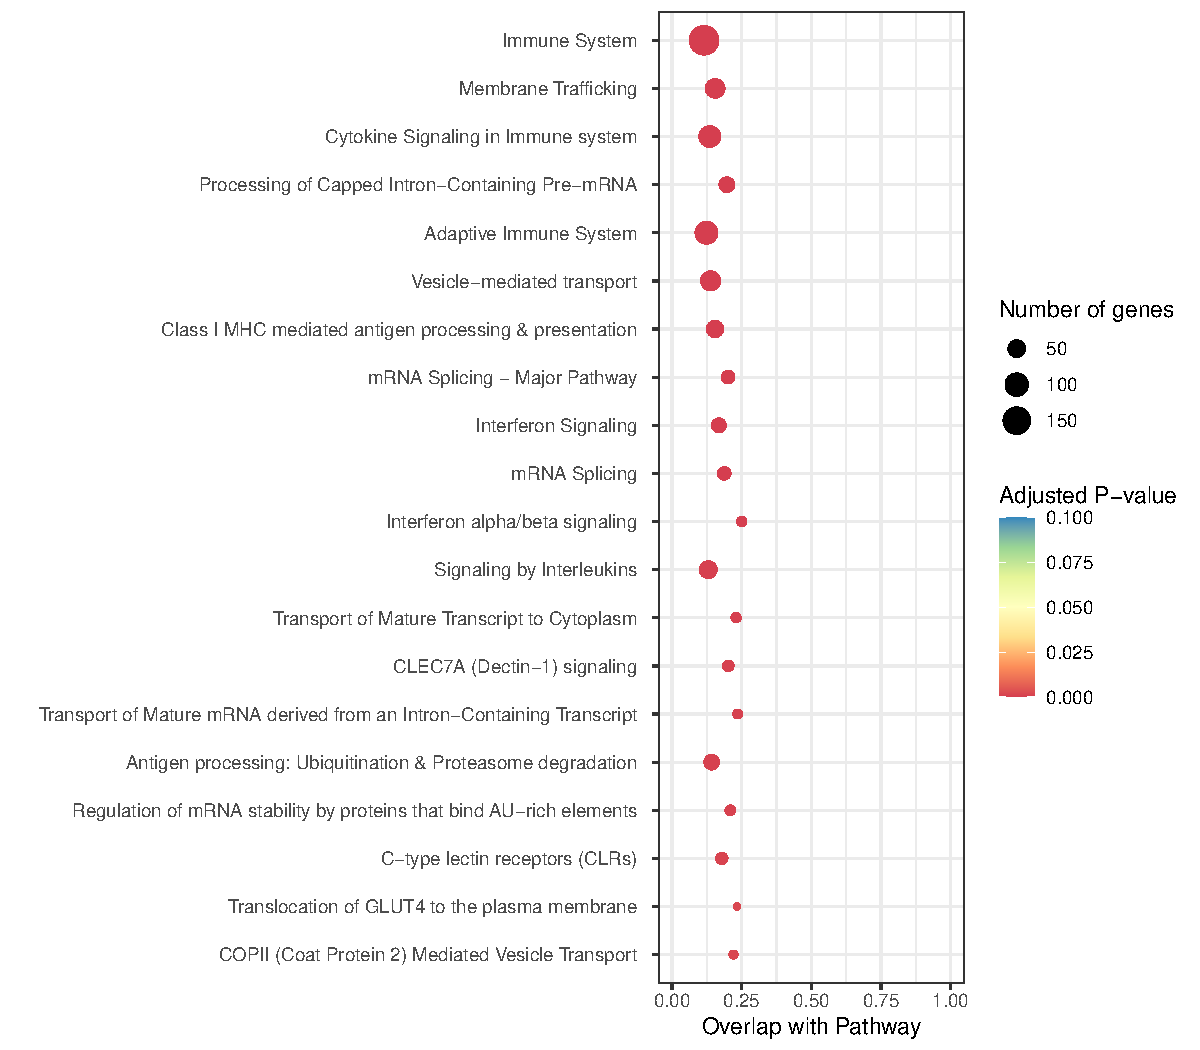
\includegraphics[width=\textwidth]{ds_sLPS_6_vs_Ctrl_6}
  \caption[REACTOME pathways enriched in differentially spliced genes (sLPS\_6 versus Ctrl\_6)]{Top 20 REACTOME pathways enriched in differentially spliced genes between Ctrl\_6 and sLPS\_6. Enriched pathways are shown on the y-axis and the overlap between differentially spliced genes and all genes in the pathway are shown on the x-axis. Colors indicate the enrichment adjusted P-values and the size of the points indicate the number of genes in each enriched pathway.}
  \label{fig:ds_sLPS_6_vs_Ctrl_6}   
\end{figure}

Stimulation with dsRNA viral mimic PolyI:C (PIC\_6) also led to dramatic splicing changes (Figure \ref{fig:ds_PIC_6_vs_Ctrl_6}). For example, genes involved in viral sensing and RIG-I/MDA5-mediated activation of the antiviral cytokine Interferon $\beta$ (IFN$\beta$) were differentially spliced (P-value=$1.7\times10^{-5}$; 7 genes). RIG-I/MDA5 receptors belong to the RIG-I-like family of receptors which sense dsRNA and activate type I interferons in response (e.g. IFN$\beta$) \cite{Yoneyama2005-ba,Kato2005-ie}. In addition to the genes coding for the RIG-I and MDA5 receptors (\textit{DDX58} and \textit{IFIH1} respectively), genes that regulate the expression of cytokine IFN$\beta$, such as \textit{TRIM25} \cite{Castanier2012-io}, \textit{TANK} \cite{Al_Hamrashdi2022-pr}, and \textit{RIPK1} \cite{Saleh2017-fv} were also differentially spliced. These observations reinforce previous functional work that showed the modulated antiviral response of RIG-I/MDA5-mediated IFN$\beta$ activation pathway by the different isoforms of its constituent components \cite{Gack2009-nw,Liao2021-aj,Lad2008-jd}. \\



\begin{figure}[H]
  \centering
  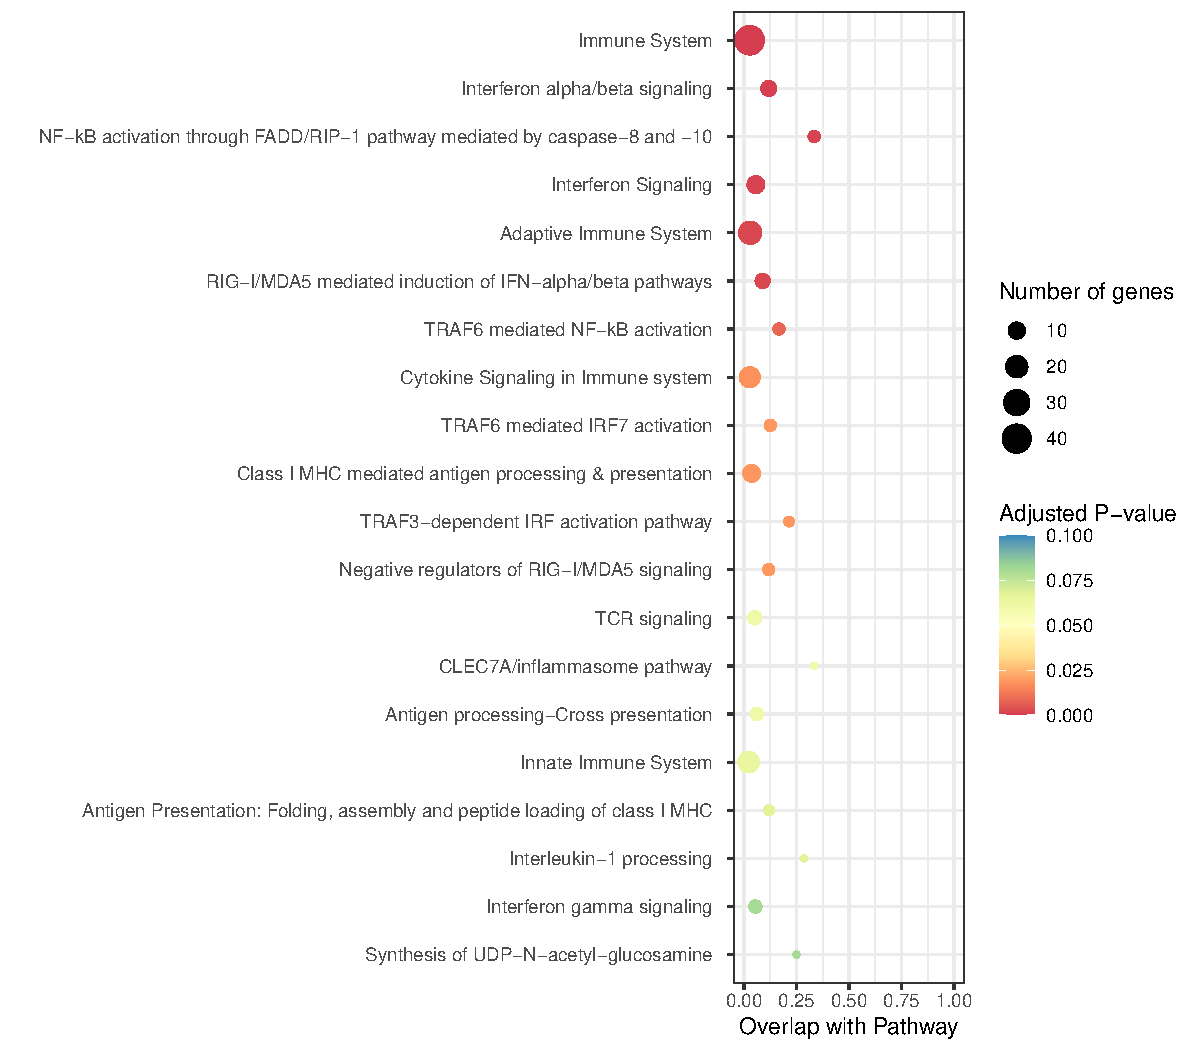
\includegraphics[width=\textwidth]{ds_PIC_6_vs_Ctrl_6}
  \caption[REACTOME pathways enriched in differentially spliced genes (PIC\_6 versus Ctrl\_6)]{Top 20 REACTOME pathways enriched in differentially spliced genes between Ctrl\_6 and PIC\_6. Enriched pathways are shown on the y-axis and the overlap between differentially spliced genes and all genes in the pathway are shown on the x-axis. Colors indicate the enrichment adjusted P-values and the size of the points indicate the number of genes in each enriched pathway.}
  \label{fig:ds_PIC_6_vs_Ctrl_6}   
\end{figure}

This study is not the first to demonstrate the important but underappreciated role of alternative splicing in innate immune response \cite{Wagner2021-fl,Kalam2017-qa}. For example, Kalam et al. \cite{Kalam2017-qa} showed that a shorter isoform of \textit{RAB8B} is expressed in macrophages upon stimulation with Mycobacterium tuberculosis. Their work showed a subtle mechanism whereby the survival of mycobacteria inside macrophages was controlled by expressing long or short isoforms of \textit{RAB8B}, which affected the ability of lysosomes to target mycobacteria. Although a detailed account of the different alternative splicing patterns in response to pathogens is not the primary focus of this chapter, it reinforces its relevance to innate immune response. It also shows that iPSC-derived macrophages are a suitable model that captures relevant transcriptomic changes upon macrophage stimulation. This analysis served as a motivation to understand the genetic regulation of alternative splicing by mapping splicing QTLs.\\
% The differential splicing analysis reinforces the role of alternative splicing in regulating important innate immunity processes (e.g. vesicle-mediated transport and viral sensing and response), but also highlights the specificity of splicing junction usage in response to specific stimuli. Although the role of alternative splicing in response to stimuli has been previously reported \cite{Wagner2021-fl}, this comprehensive and well-powered screen captures pathway-level changes in splice junction usage in response to a broad range of stimuli. Furthermore, these findings demonstrate that iPSC derived macrophages can faithfully recapitulate known biological pathways activated by different stimuli. This motivated me to investigate how genetic variation affects alternative splicing in macrophages and how such genetic variation may, in turn, predispose to IMDs.\\

\subsection{Macrophage stimulation increases the number of genes with significant sQTL effects }




After intron usage quality control, I identified a median of 82,058 introns per condition, with a total of 160,748 unique introns across all conditions (75,987-105,841 introns per conditions with the greatest  number of introns seen in Prec\_D0; Figure \ref{fig:qc_introns_num} in Methods). Approximately 81\% of identified introns were independently identified in at least 2 conditions (Figure \ref{fig:dist_intron_num}). Interestingly, 53\% of single-condition introns were identified in Prec\_D0. This finding is in line with the earlier correlation analysis that showed that intron usage correlation between undifferentiated iPSCs and differentiated macrophages is generally weaker than intron usage ratio correlation among differentiated macrophages (Figure \ref{fig:cond_corr}). Furthermore, it shows that a largely distinct set of splice junctions are used in undifferentiated iPSCs that become undetectable in fully differentiated macrophages. \\

\begin{figure}[H]
  \centering
  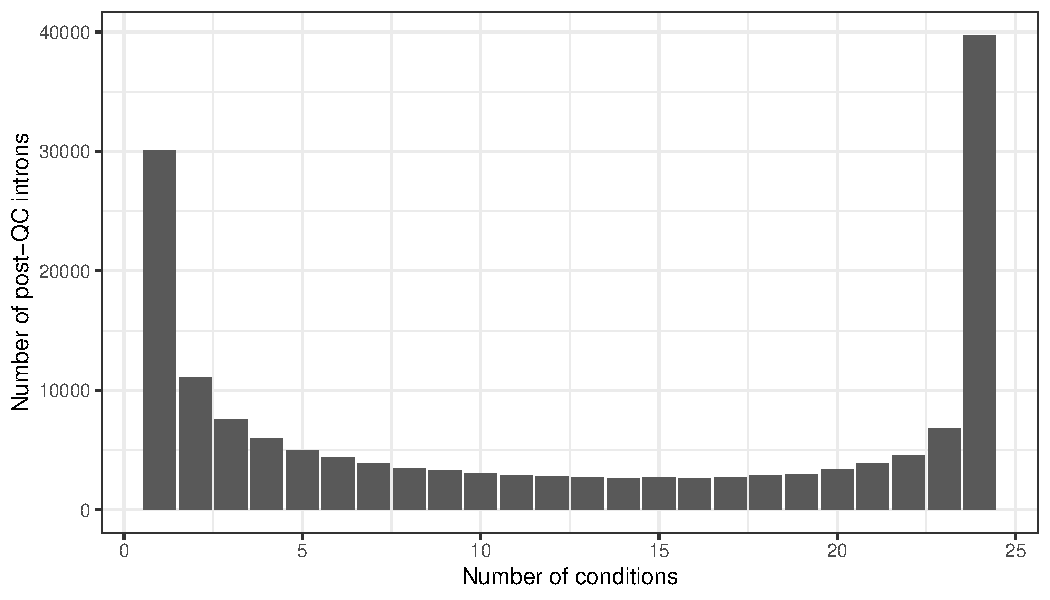
\includegraphics[width=0.8\textwidth]{dist_intron_num}
  \caption[Number of introns that passed QC versus the number of conditions where introns passed QC]{Distribution of the number of introns that were detected and passed QC in different numbers of conditions.}
  \label{fig:dist_intron_num}   
\end{figure}
After mapping the quantified introns to genes (see section \ref{sec:intron_qc_methods} in Methods for details), I found that each gene had a median of seven introns and up to 10,851 genes were quantified per condition. In total, introns were mapped to 12,792 genes across all conditions, and over 94\% of genes were detected in at least 2 conditions (Figure \ref{fig:dist_gene_num}). Similar to introns, over half of the 6\% single-condition genes were unique to Prec\_D0.

\begin{figure}[H]
  \centering
  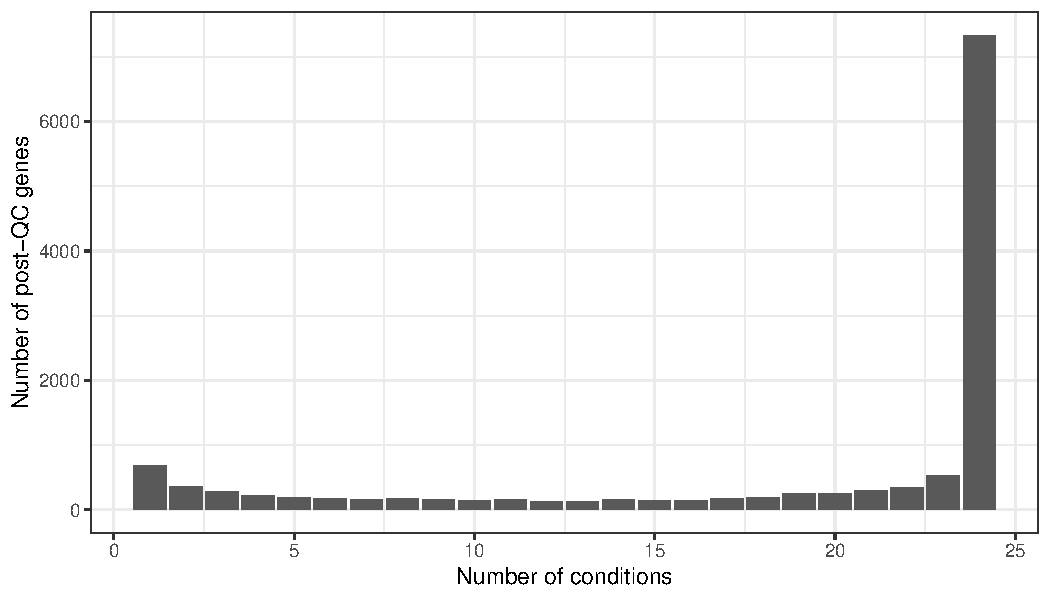
\includegraphics[width=0.8\textwidth]{dist_gene_num}
  \caption[Number of genes with introns that passed QC versus the number of conditions where genes passed QC]{Distribution of the number of genes that were detected and passed QC in different numbers of conditions.}
  \label{fig:dist_gene_num}   
\end{figure}
% Intron usage ratios were normalised (quantile normalised and rank-based inverse normal transformed) and introns with low variance (standard deviation < 0.005), or intron clusters without split reads in more than 40\% of samples, were excluded (Methods). I identified a median of 82,058 introns (75,987-105,841 introns across conditions with the greatest  number of introns seen in Prec\_D0; Figure \ref{fig:qc_introns_num} in Methods). Each gene had a median of 7 introns and up to 10,851 genes were quantified per condition. \\

Using normalised intron usage ratios as normally distributed quantitative traits, sQTLs were mapped within a $\pm$ 1 Mbp window centred around the transcription start site (TSS) of each gene. I also used multivariate adaptive shrinkage (mash \cite{Urbut2019-gf}) to compare sQTL effect sizes between naive and stimulated conditions (I used Ctrl\_24 as a baseline condition). Mash reports a significance measure known as local false sign rate (LFSR; section \ref{sec:mash_methods} in Methods), which I used to identify sQTLs whose effect sizes change significantly upon stimulation (response sQTLs). \\

I called significant sQTLs at a false discovery rate (FDR) < 0.05. Across all conditions, I detected a total of 5,734 sGenes (median number of sGenes per condition=1580 and Prec\_D2 had the most sGenes=1,881) (Figure \ref{fig:sqtl}a,b). Of these, 878 sGenes (15.3\%) had at least one response sQTL (LFSR < 0.05).  As expected, Prec\_D2, Ctrl\_6, IL4\_6, and IL4\_24 had the smallest proportion of response sQTLs (< 9\%). This is expected because Prec\_D2 and Ctrl\_6 represent naïve macrophages and it is therefore unlikely that any significant transcriptomic changes will have occurred when their RNA was harvested. Similarly, stimulation with the anti-inflammatory cytokine IL4 is unlikely to result in any significant response sQTLs, consistent with results from the differential splicing analysis where stimulation with IL4 led to the smallest number of differentially spliced genes across all conditions.\\

I then asked which of the two stimulation timepoints (6 and 24 hours) was more likely to have response sQTL effects across stimulation conditions. Up to 29\% of response sGenes per condition had a response sQTL after 24 hours that was not detected after 6 hours. Conversely, up to 72\% of response sGenes per condition had a response sQTL after 6 hours that was  undetectable after 24 hours. This suggests that response sQTLs are more likely to be detected 6 hours after stimulation (Figure \ref{fig:sqtl}c), in agreement with previous work that suggested 4-6 hours for optimal detection of transcriptomic changes following macrophage stimulation \cite{Unuvar_Purcu2022-zq,Sharif2007-np}. \\
\begin{figure}[H]
  \centering
  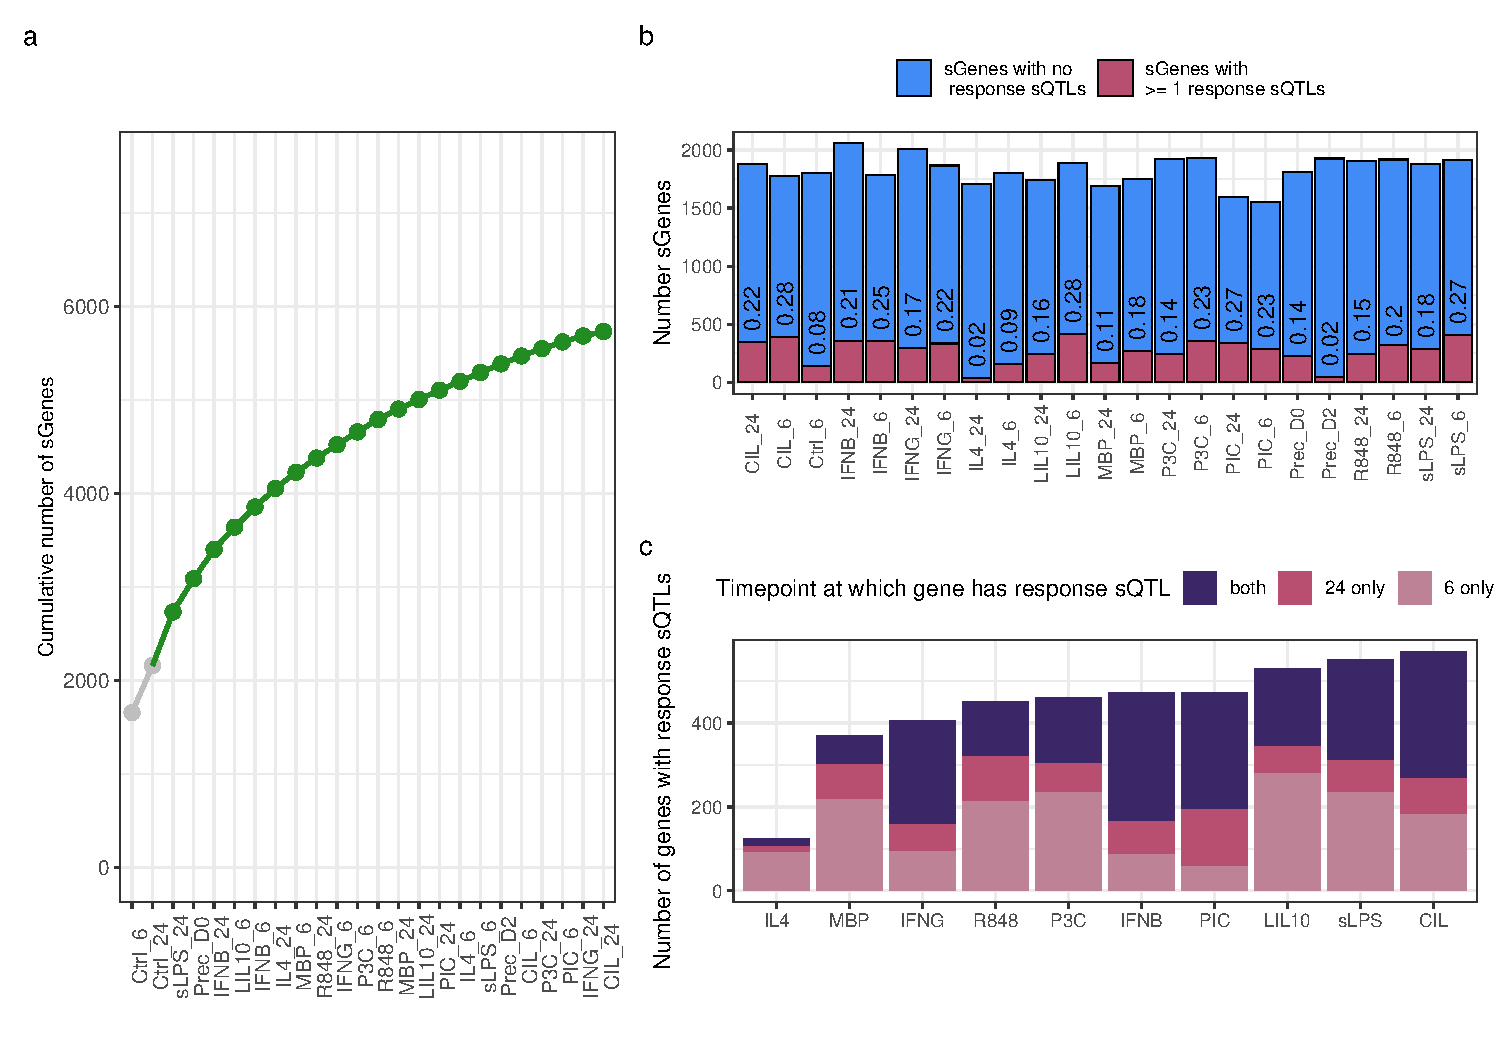
\includegraphics[width=\textwidth]{sqtl}
  \caption[Splicing QTL mapping, timepoint-specificity and condition-specificity results]{(a) Cumulative number of genes with significant splicing QTL effects, with unstimulated conditions indicated in grey (b) Total number of significant sQTLs per condition and proportion of response sQTLs within each condition (sQTLs with LFSR < 0.05; Methods). (c) Number of genes, per condition, with at least one response sQTL at 6 hours, 24 hours or both.}
  \label{fig:sqtl}   
\end{figure}

Similar to previous reports \cite{Garrido-Martin2021-sk}, I found that lead sQTL SNPs are located closer to intron boundaries than to the TSS of their genes. On average per condition, 24.5\% of sGenes had a lead SNP within 10 kbp of their TSS, compared to 46.8\% within 10 kbp of either the 5' or 3' intron boundaries (Figure \ref{fig:tss_esqtl}a). However, the lead SNP was located within the boundaries of its associated intron in less than 4\% of significant sQTLs. Although it is compelling to think that distal enhancer or silencer sequences may explain this observation, it is also likely that the lead SNP is an LD proxy for the truly causal SNP. The significant sQTL introns had a median length of 2.5 kbp, which is much shorter than the European-ancestry LD ranges of many loci. \\
\begin{figure}[H]
  \centering
  \begin{subfigure}[b]{0.45\textwidth}
      \centering
      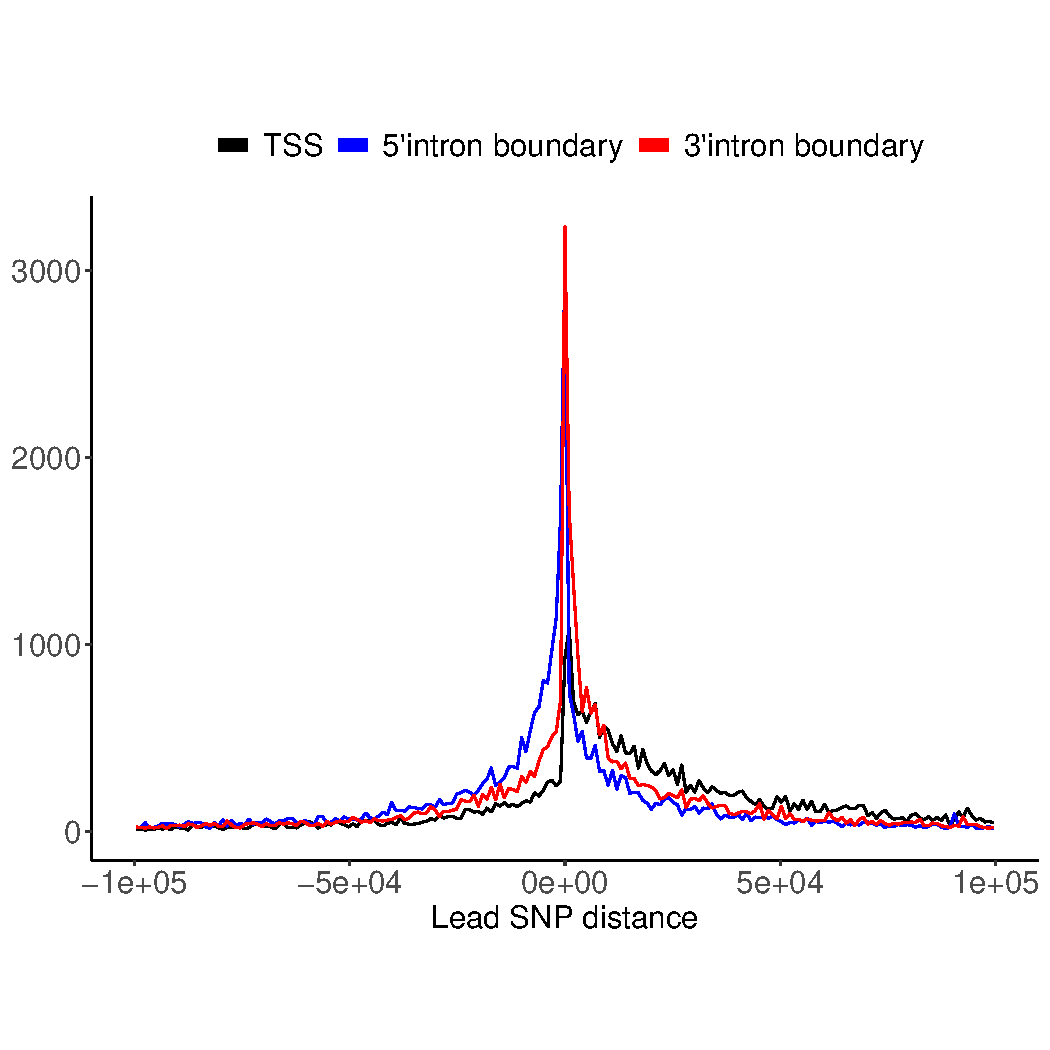
\includegraphics[width=\textwidth]{intron_tss}
      \caption{}
      \label{fig:intron_tss}
  \end{subfigure}
  \hfill
  \begin{subfigure}[b]{0.45\textwidth}
      \centering
      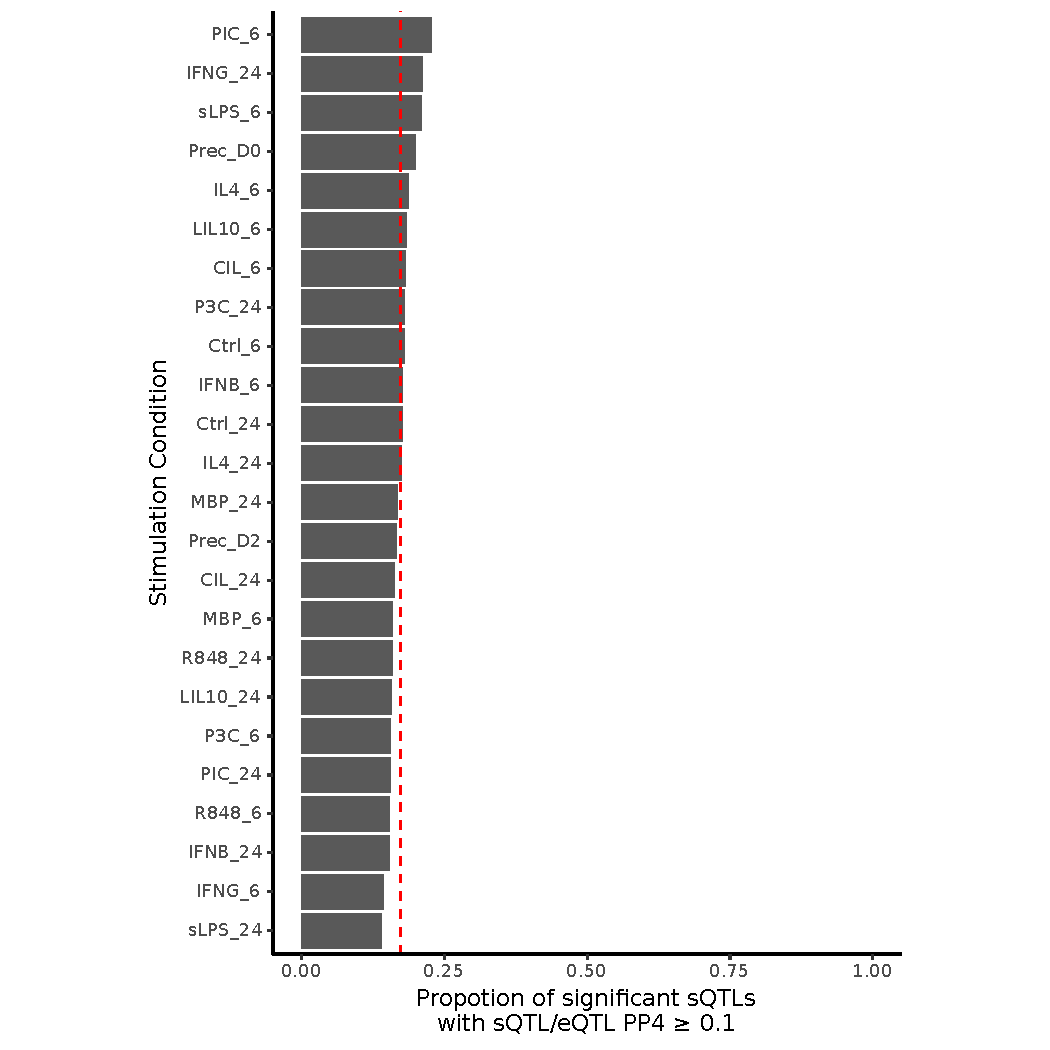
\includegraphics[width=\textwidth]{esqtl}
      \caption{}
      \label{fig:esqtl}
  \end{subfigure}


     \caption[Lead sQTL SNP position distribution and colocalisation between sQTLs and eQTLs]{(a) Distribution of the distance between the lead SNPs of significant sQTL effects (across all conditions) and transcription start site (TSS; in black) of the sQTL gene, 5'intron boundary (in blue) and 3' intron boundary (in red). (b) Proportion of significant sQTL effects that share a single causal variant (PP4 $\geq$ 0.1) with the same eQTL gene in the same condition. Red line indicates the average proportion of sQTLs with sQTL/eQTL colocalisation $\geq$ 0.1 across conditions.}
     \label{fig:tss_esqtl}
\end{figure}
I next sought to understand the relationship between the sQTL and eQTL signals at the discovered sGenes. This is an important question in the context of understanding the transcriptomic effects of disease-associated loci. If it is the case that a large proportion of sQTL signals colocalised with eQTL signals, then the added value of sQTLs in terms of explaining disease-associated loci would be limited. Existing evidence on the relationship between eQTL and sQTL signals is contradictory. While some sQTL mapping efforts have shown that sQTL signals are largely independent from eQTL signals, others maintain that there is a large overlap between eQTLs and sQTLs \cite{Garrido-Martin2021-sk,Kim-Hellmuth2020-gz,Wang2008-fb,Lappalainen2013-mz}. Therefore, it is unclear whether overall levels of gene expression and alternative splicing are genetically co-regulated or are regulated via distinct mechanisms \cite{Kim-Hellmuth2020-gz,Wang2008-fb,Lappalainen2013-mz}. To verify this, I performed statistical colocalisation (Methods; ref \cite{Giambartolomei2014-yl}) between sQTLs and eQTLs derived from the same data (Panousis et. al. 2023 \cite{macromap-eqtl}). Specifically, for all sGenes, I colocalised the sQTL and eQTL signals in the exact same window (1 mbp around TSS). I found that on average across conditions, 75\% of sGenes were extremely unlikely to share a causal variant with eQTLs from the same genes (PP4 < 0.1; Figure \ref{fig:tss_esqtl}b; Methods), indicating that the majority of sQTL signals are largely independent from eQTL signals. Building on this evidence, I therefore hypothesised that colocalisation of sQTLs with disease-associated loci may explain additional disease-associated loci distinct from those already implicated via eQTLs. \\




\subsection{Splicing QTLs identify GWAS effector genes undetected by expression QTLs}


I then aimed to identify IMD-associated loci that were likely linked to alternative splicing changes in macrophages. To this end, I used statistical colocalisation analysis between sQTL and GWAS association signals (using R package coloc; more details in Methods). Since macrophages play a major role in innate immune defence, I focussed on 21 IMD GWAS summary statistics to quantify the probability of a sQTL sharing a causal variant with genetic association signals. IMD GWAS summary statistics were downloaded from the GWAS catalogue \cite{Buniello2019-wb} (See methods for how GWAS loci were defined and Table \ref{tab:gws_studies} for a complete list of downloaded GWASes). In order to compare the colocalisation yield between eQTLs and sQTLs, I also obtained colocalisation results from eQTLs mapped from the same dataset and colocalised with the same GWAS loci.\\


Across all 21 IMDs, 1,528 GWAS loci were tested against 4490 genes across all conditions (34,128 introns). I identified 707 unique genes (1,337 introns) with an sQTL signal in at least one condition that likely shares a causal variant with an IMD risk locus (PP4 $\geq$ 0.75; Figure \ref{fig:coloc_cum_response_sqtl}). Approximately, 60\% of these genes passed the colocalisation threshold in a single condition only. However, these should not be interpreted as condition-specific colocalisations as the PP4 values could be close to the colocalisation threshold in other conditions. Therefore, I compared the effect sizes of the colocalised sQTL across all condition using mash. I observed that 68 (9.6\%) of the colocalisaed genes implicated a response sQTL, indicating that the genetic effects of these variants on alternative splicing could not be detected in unstimulated macrophages. Based on hierarchical clustering of LFSR values, Prec\_D2, IL4\_6 and IL4\_24 had the fewest response sQTLs that colocalised with GWAS signals, while sLPS\_6, CIL\_6 and LIL10\_6 (all stimulated with LPS) yielded the most, recapitulating results from the differential splicing analysis (Figure \ref{fig:coloc_cum_response_sqtl}). \\

\begin{figure}[H]
  \centering
  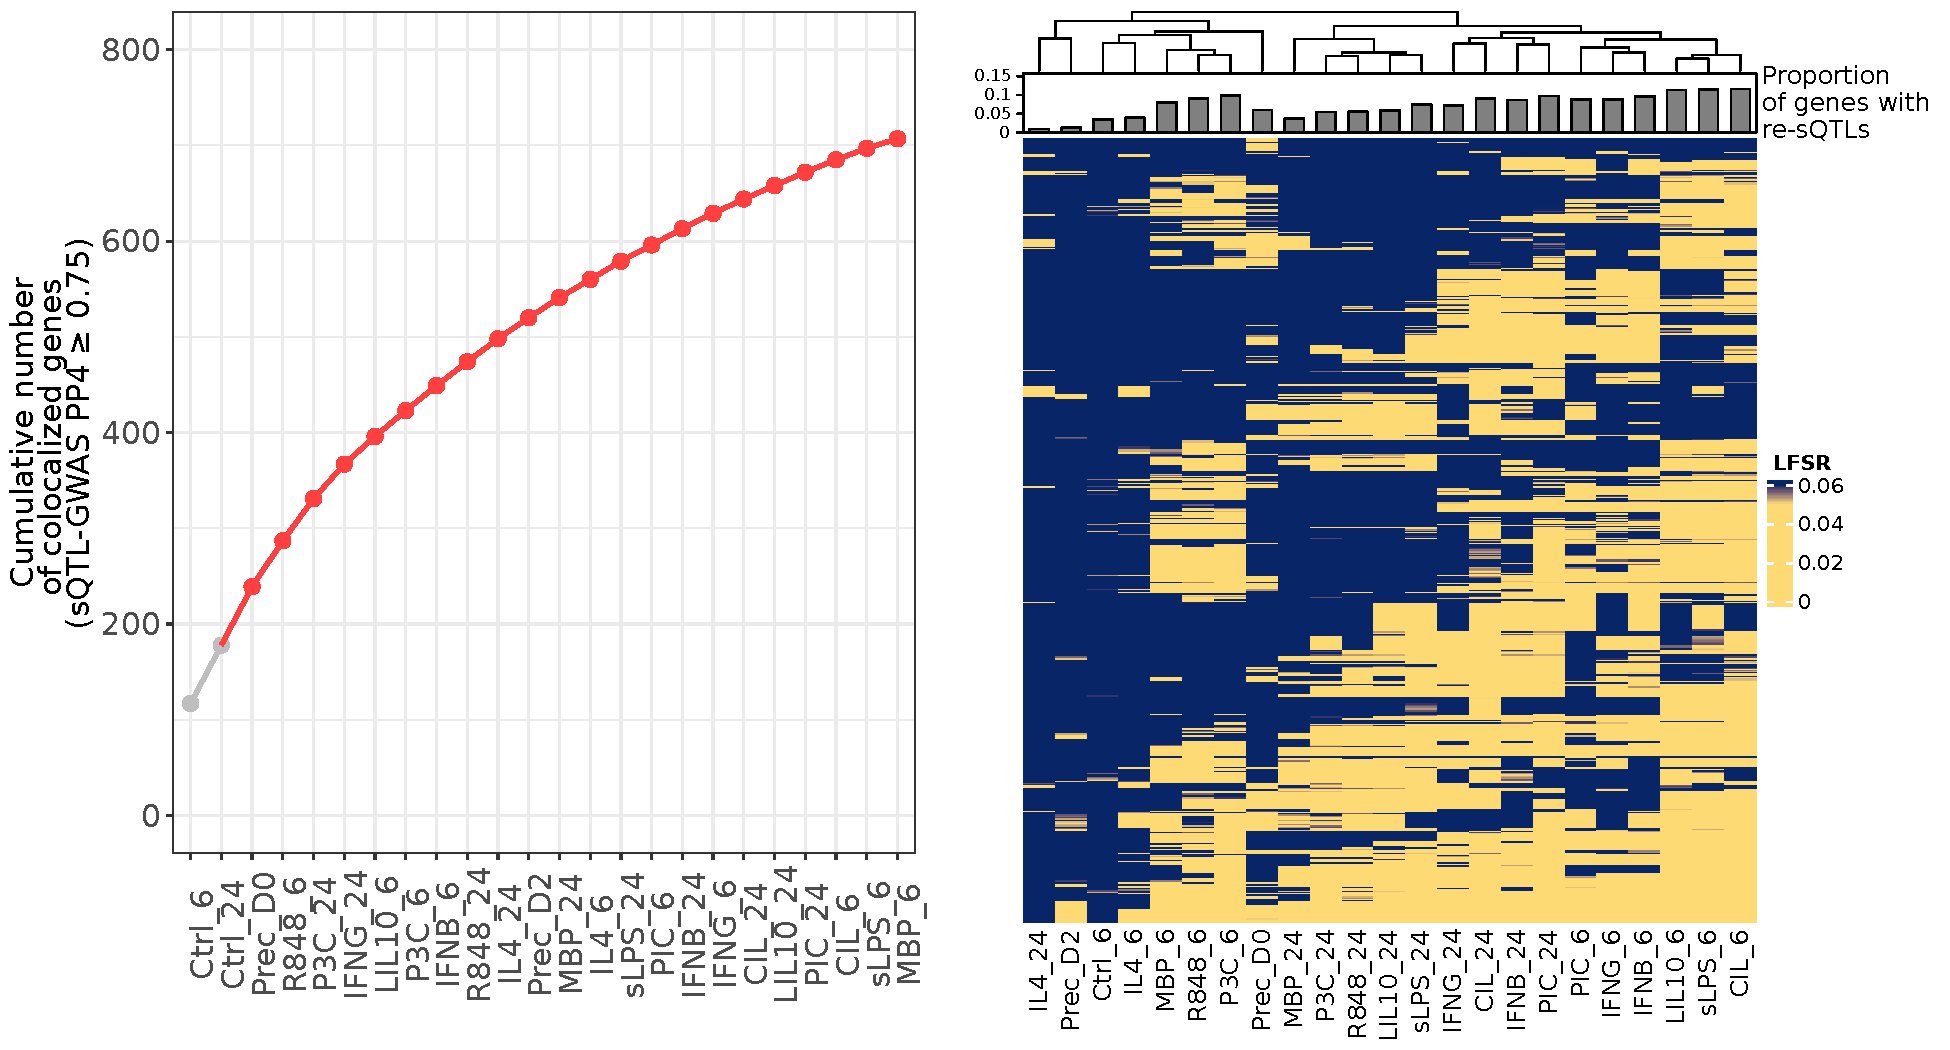
\includegraphics[width=\textwidth]{coloc_cum_response_sqtl}
  \caption[Condition-specificity of colocalised sQTLs]{(left) Cumulative number of genes with a GWAS-sQTL (PP4 $\geq$ 0.75) across different conditions, with unstimulated conditions shown in grey on the left. (right) Heatmap and hierarchical clustering of LFSR values for all the colocalised sQTL effects (PP4 $\geq$ 0.75) across all 21 IMDs. On top of the heatmap is a barplot showing the proportion of colocalised sQTL effects that are response sQTLs (LFSR < 0.05)}
  \label{fig:coloc_cum_response_sqtl}   
\end{figure}
I then compared how many tested loci colocalised with each type of molecular QTL and found that 50.4\% (771/1,528) of tested loci were likely to share a single causal variant with either an eQTL, sQTL or both. Recently, Mountjoy et al. 2021 (ref: \cite{Mountjoy2021-fc}) colocalised 50.7\% of tested GWAS loci with protein and expression QTLs from 92 tissues and cell types. In comparison, this high colocalisation yield from a single cell type shows the promise of profiling the transcriptome of a relevant cell type in understanding the effects of GWAS loci. Moreover, unlike other tissue-level QTL maps, interpreting these colocalisations in the context of macrophages potentially aids the interpretation and functional follow-up of these loci. \\

Approximately half of the colocalised loci (385 loci or 25.2\% of tested loci) colocalised solely with an sQTL (sQTL PP4 $\geq$ 0.75 > eQTL PP4), clearly demonstrating both the value of sQTLs for identifying GWAS effector genes and the important role that alternative splicing plays in complex disease risk (Figure \ref{fig:macromap_esqtl_total_loci}). However, this percentage may also be affected by eQTL colocalisations that are close to the colocalisation threshold (e.g. eQTL PP4 = 0.74). When I relaxed the eQTL PP4 threshold (sQTL PP4 $\geq$ 0.75 and eQTL PP4 $\geq$ 0.5), I found that 16.8\% of loci colocalised solely with an sQTL signal.  On the other hand, at the same thresholds applied in reverse (i.e. eQTL PP4 $\geq$ 0.75 and sQTL PP4 $\geq$ 0.5), only 2\% of loci colocalised solely with an eQTL signal.\\
\begin{figure}[H]
  \centering
  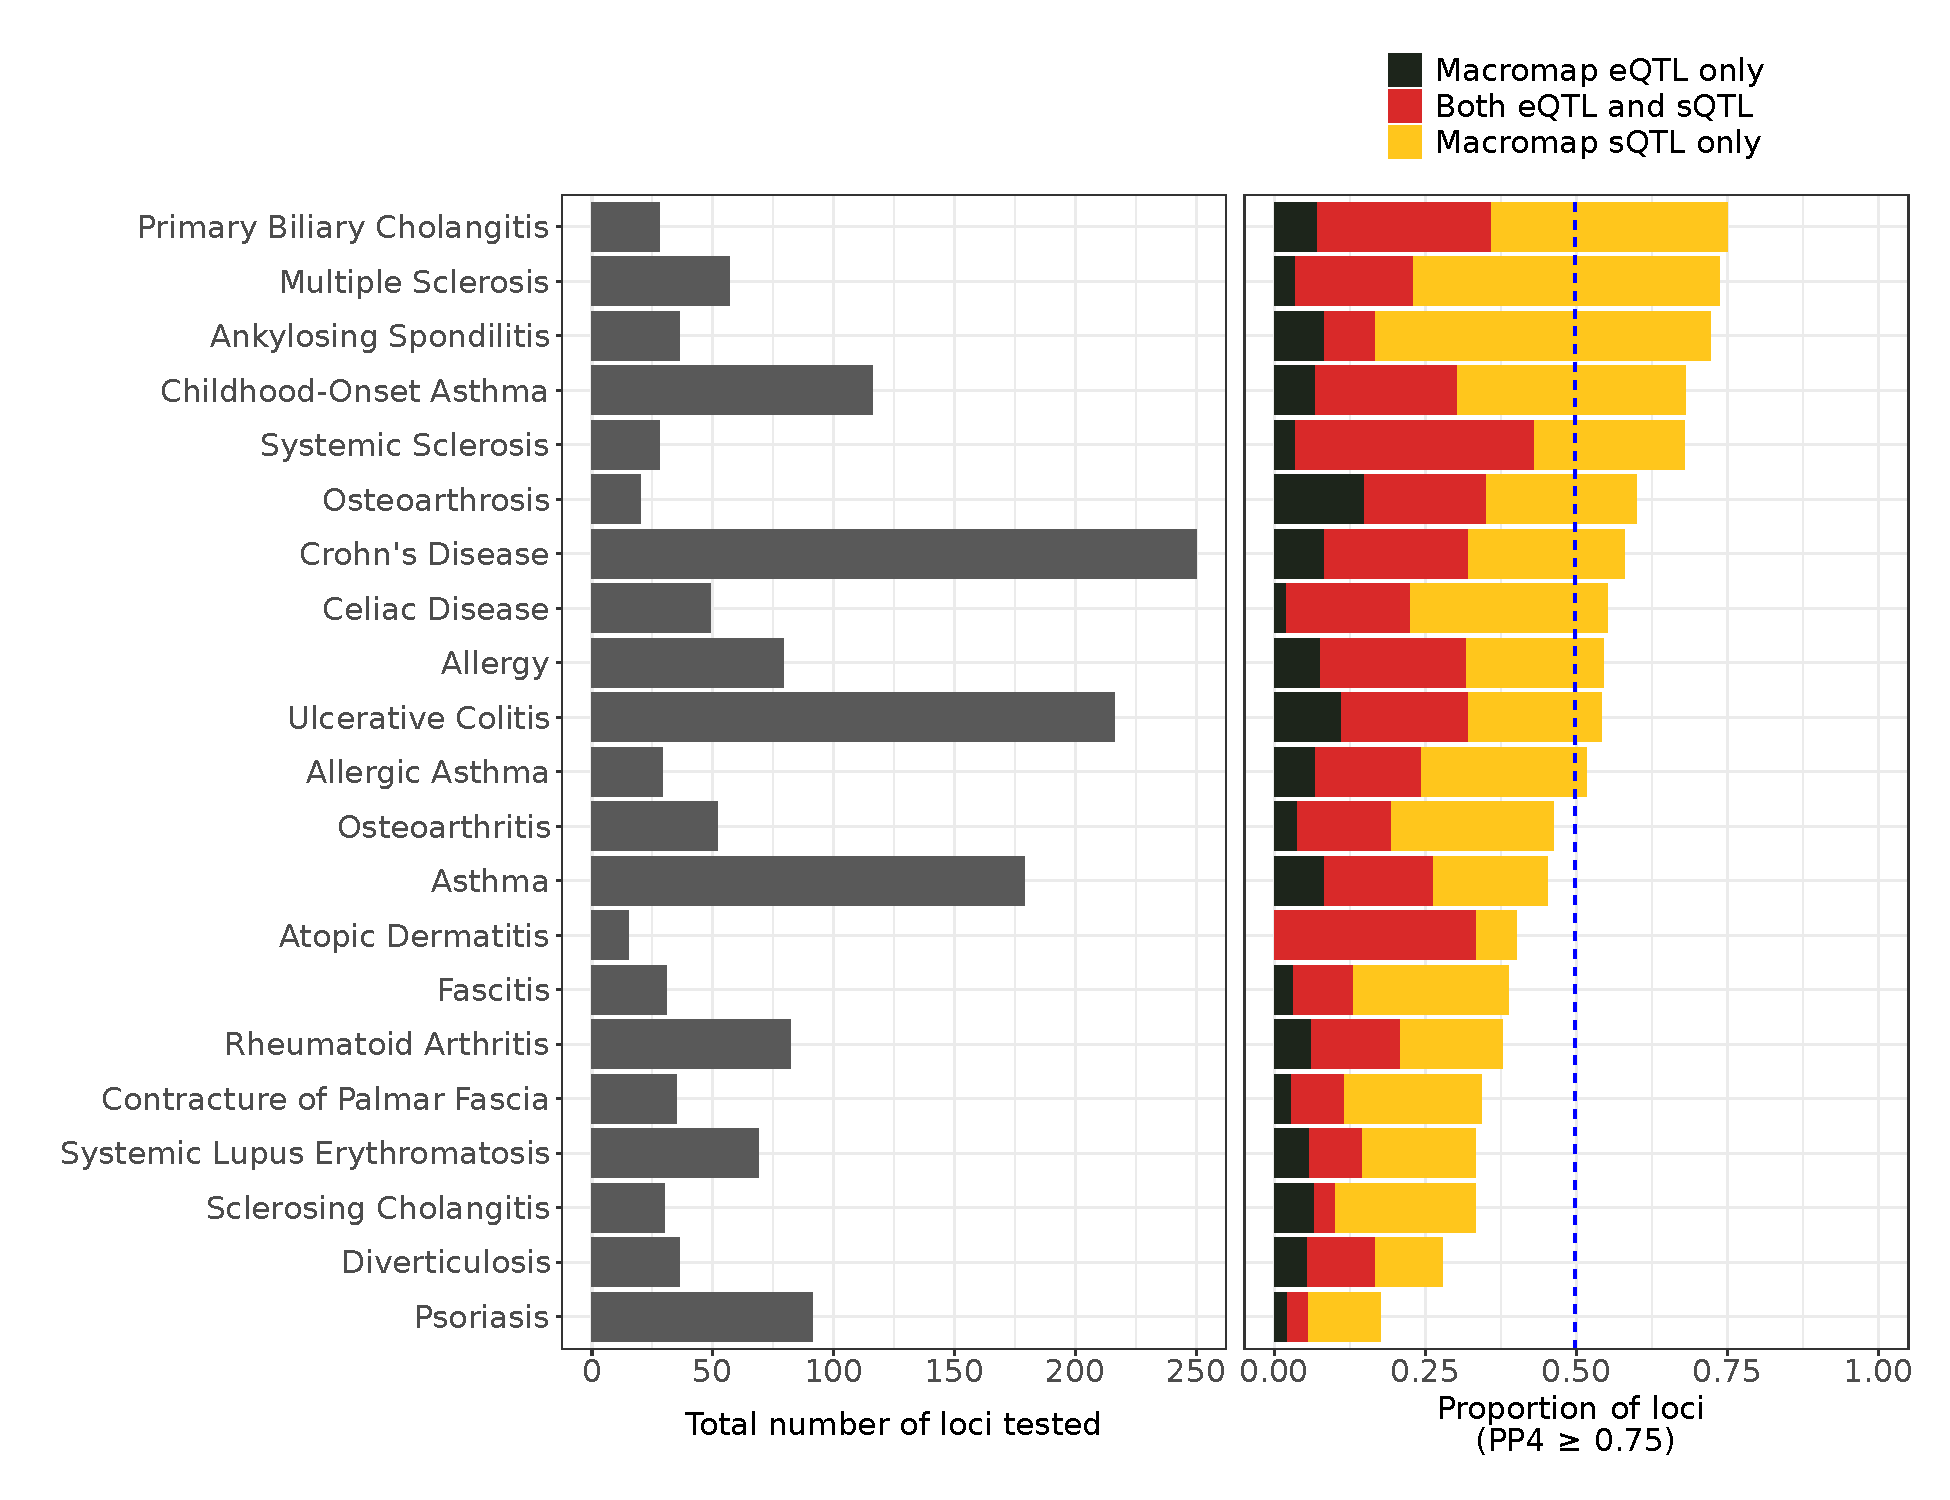
\includegraphics[width=\textwidth]{macromap_esqtl_total_loci}
  \caption[Colocalisation analysis results across 21 immune-mediated diseases]{Total number of loci tested for colocalisation (left) and proportion of genome-wide significant loci that share a single causal variant (PP4 $\geq$ 0.75) with an eQTL only, an sQTL only or both (right).}
  \label{fig:macromap_esqtl_total_loci}   
\end{figure}
\subsection{Lowly-used alternative splicing events underlie complex disease risk}
\begin{figure}[H]
  \centering
  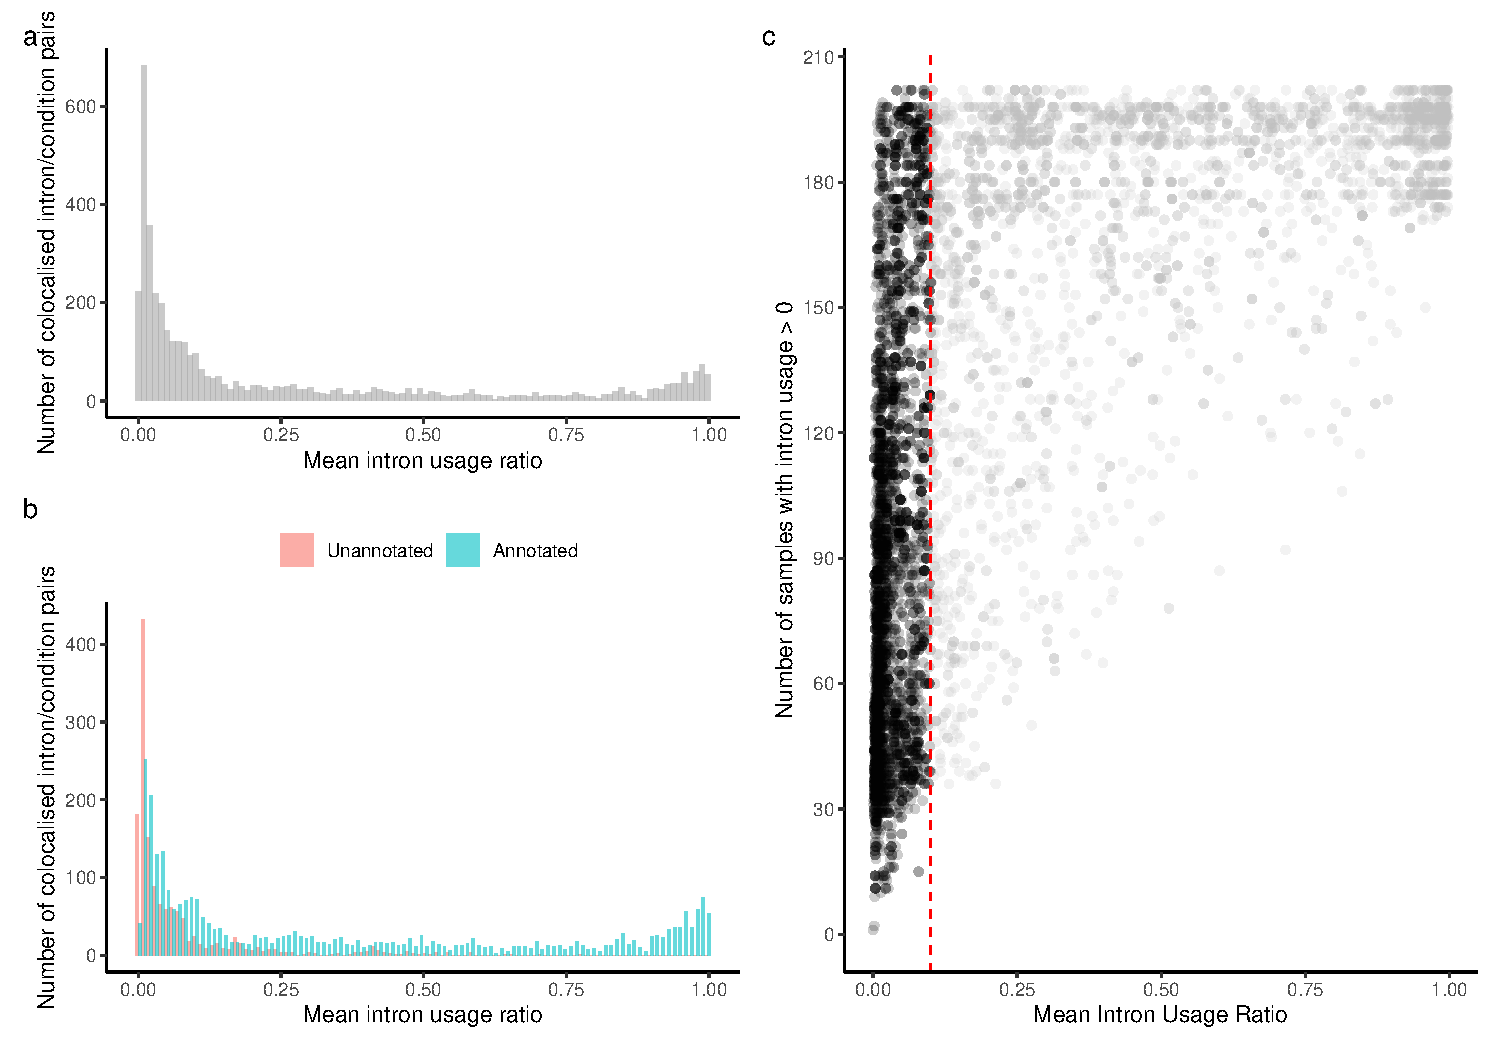
\includegraphics[width=\textwidth]{low_sj}
  \caption[Intron usage of colocalised introns]{(a) Distribution of mean intron usage ratio for colocalised introns, showing a peak close to 0, and (b) coloured by annotation in GENCODE v27, showing an enrichment of unannotated introns among introns with low mean usage ratio (c) Number of samples in which the intron is supported by split reads (y-axis) shown against the mean intron usage ratio of each sample (x-axis). Red vertical line at mean intron usage ratio  = 0.1.}
  \label{fig:low_sj}   
\end{figure}
I next sought to characterise the colocalised sQTL introns, by asking how often colocalised sQTL splicing events are used in observed transcripts. There is ample evidence that aberrant splicing underpins several inherited diseases such as Spinal Muscular Atrophy and Duchenne Muscular Dystrophy \cite{Symoens2011-ew,Abramowicz2018-by,Sanz2017-re}, but it is unclear to what extent lowly-observed splicing events contribute to complex diseases. To evaluate this role, I assessed the usage of introns that were implicated in IMD risk via colocalisation analysis. \\

I observed that 53.4\% of colocalised sQTL introns have a mean intron usage ratio (IUR) < 0.1 across samples (Figure \ref{fig:low_sj}a). Over 96\% of these introns had non-zero usage in at least 30 samples (Figure \ref{fig:low_sj}c), indicating that these splicing events can be reliably observed in multiple RNA-seq samples and individuals, but with relatively low IUR. Moreover, 50.6\% of these introns are not found in any annotated transcripts in GENCODE v27, whereas only 12\% of introns with mean IUR $\geq$ 0.1 are absent from GENCODE v27 (Figure \ref{fig:low_sj}b), in line with previous reports showing that lowly-observed splicing events tend to be unannotated in transcript databases \cite{Nellore2016-fj,Pickrell2010-lz}. \\

The observation that over half of colocalised sQTL introns are lowly used and that they tend to be unannotated strongly emphasises the need to investigate their functions and role in the context of complex disease. For example: are low-abundance transcripts translated into protein products or do they exert gene regulatory functions? What is the effect of up- or down-regulating these isoforms on different cellular phenotypes? Sampling these rare transcripts will thus shed light on the transcriptomic effects of IMD-associated risk loci, an avenue that has remained largely unexplored in most large-scale transcriptomic cohorts. \\
\subsection{A rare alternative splicing event likely underpins IBD risk at the \textit{PTPN2} locus}

\begin{figure}[H]
  \centering
  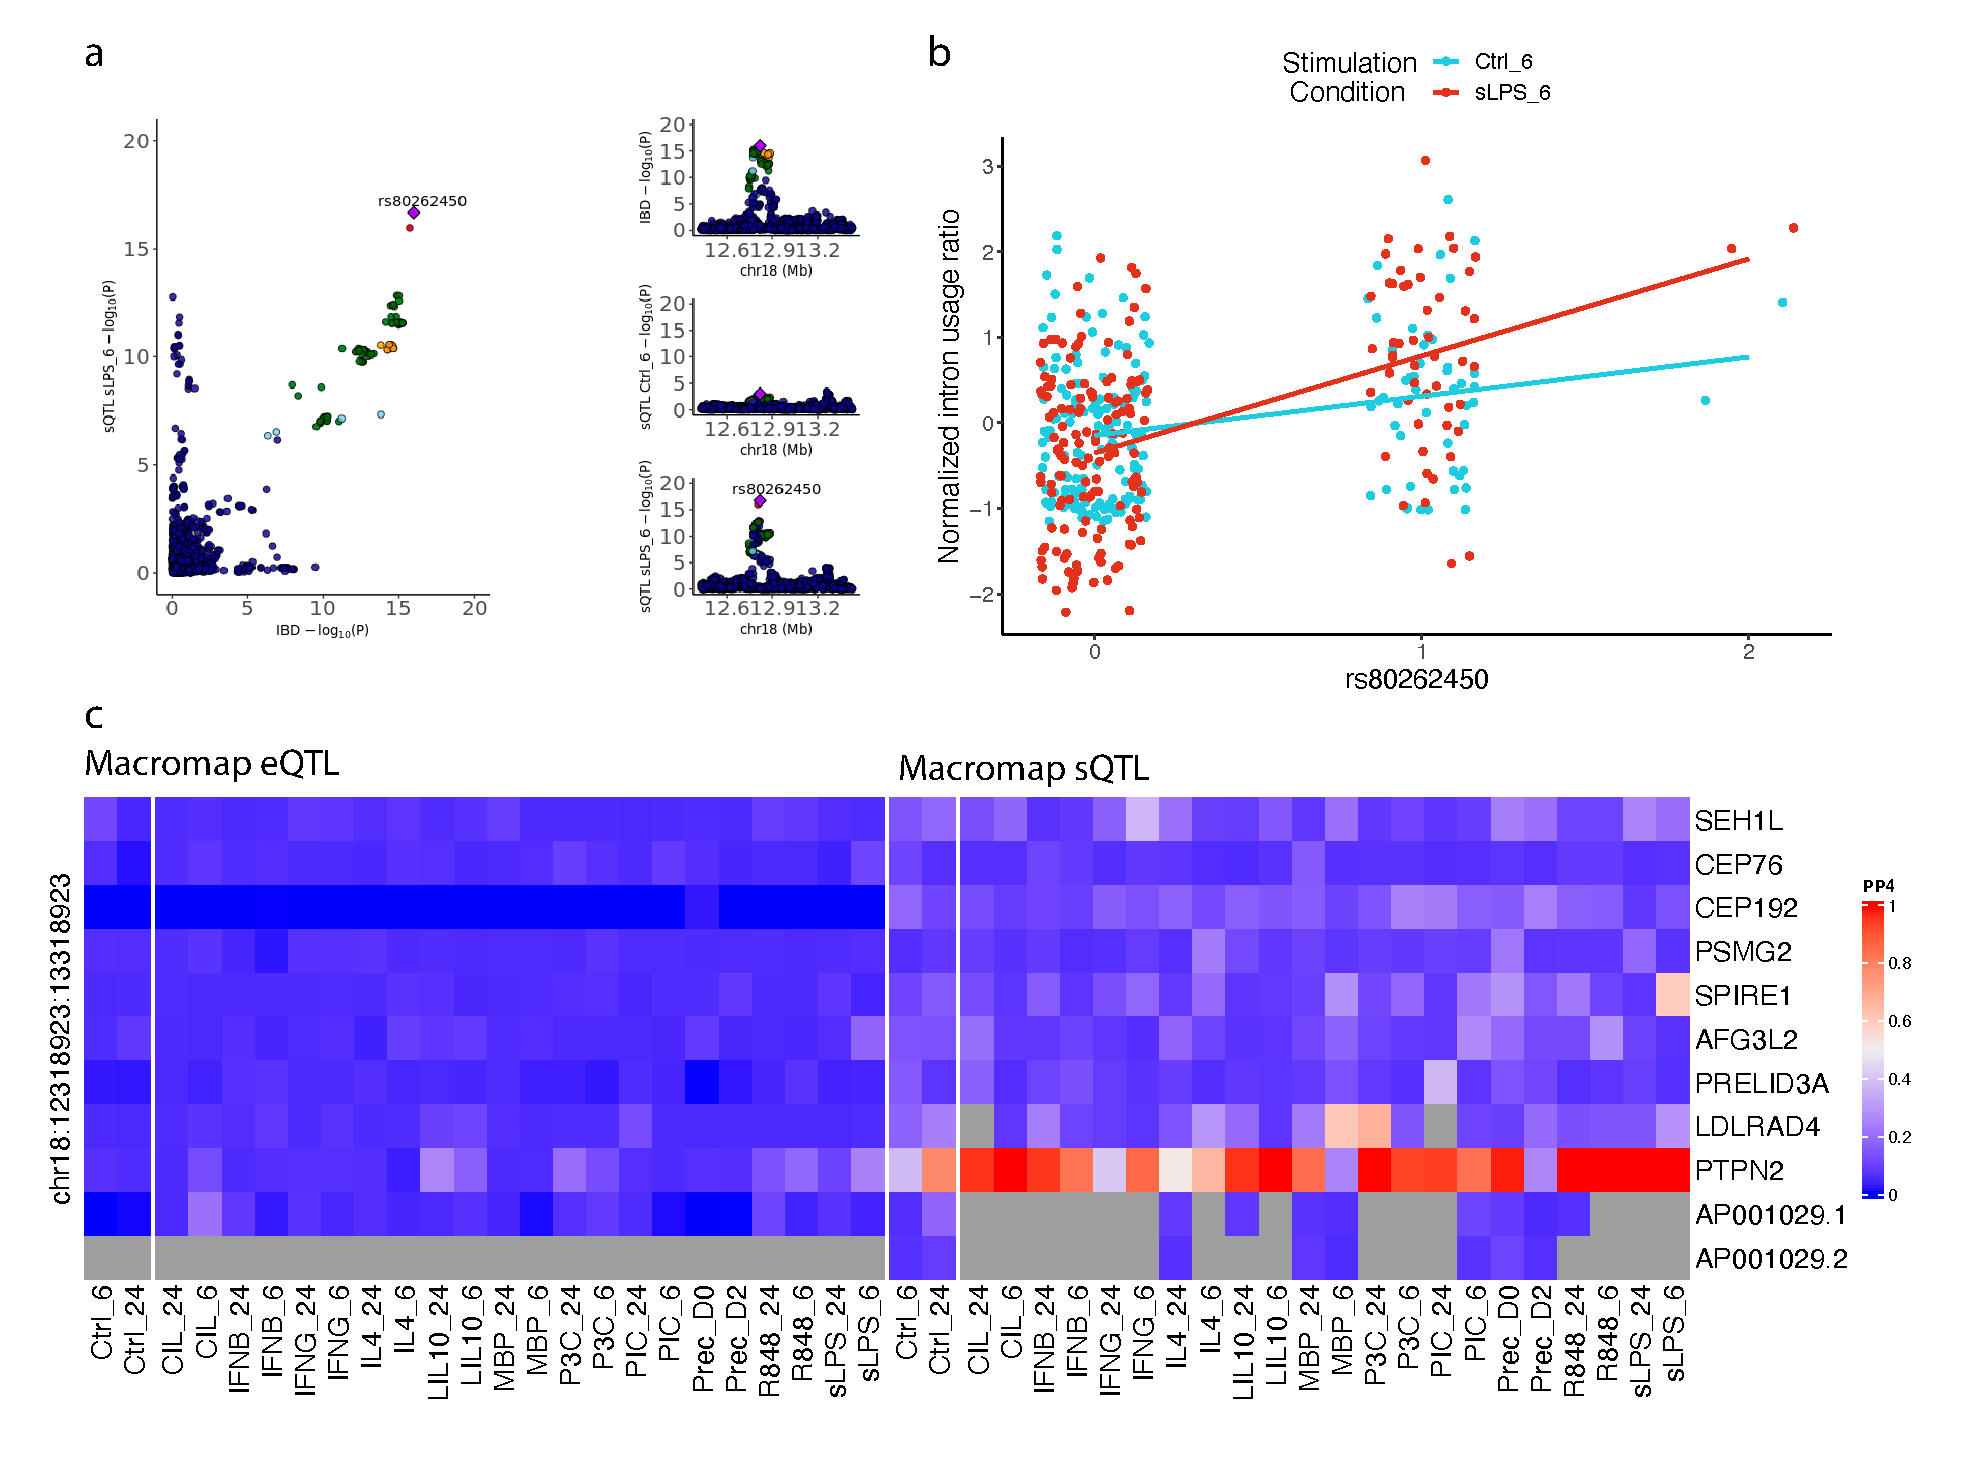
\includegraphics[width=0.9\textwidth]{ptpn2_manhattan_heatmap}
  \caption[Colocalisation between a low-usage \textit{PTPN2} intron and an IBD-associated locus]{Example of colocalisation between an IBD risk locus at 18p11.21 and an sQTL for \textit{PTPN2}.  (a) Regional association plots of the IBD association signal, and sQTL association signal in unstimulated macrophages (Ctrl\_6) and macrophages stimulated with sLPS after 6 hours (sLPS\_6), (b) Normalised intron usage ratios of different genotypes of the lead IBD SNP rs80262450 in Ctrl\_6 and sLPS\_6, (c) Heatmap showing evidence of colocalisation (PP4) between the IBD association signal at 18p11.21 and all macrophage eQTLs/sQTLs in the locus (in all conditions).}
  \label{fig:ptpn2_manhattan_heatmap}   
\end{figure}
To demonstrate how sQTLs for lowly-used introns can dysregulate alternative splicing and predispose to IMDs, I further investigated a \textit{PTPN2} sQTL that implicates a lowly-used intron that colocalised with an inflammatory bowel disease (IBD) associated risk locus at 18p11.21. Multiple lines of evidence, including coding variants associated with monogenic IBD \cite{Parlato2020-lh,Pike2018-wn} and mouse knock-out models \cite{Spalinger2018-mb,Spalinger2022-xj}, have suggested \textit{PTPN2} is the effector gene at 18p11.21, though this remains to be established. It is not yet known if and how common IBD-associated SNPs affect the expression of \textit{PTPN2}. \\

I observed that the lead IBD SNP at 18p11.21 (rs80626450; 18:12818923\_G\_A) is associated with higher risk of IBD and with increased usage of intron 1-2 of the non-canonical transcript \textit{PTPN2-205} (chr18:12,817,365-12,818,944; Figure \ref{fig:ptpn2_manhattan_heatmap}b and  Figure \ref{fig:ptpn2_sashimi}). rs80626450 is located 21 base pairs downstream of the donor splice site of exon 1 of \textit{PTPN2-205}, and is the lead SNP for both the sQTL and IBD association signals, strongly suggesting its involvement in the aberrant splicing event at this locus (Figure \ref{fig:ptpn2_manhattan_heatmap}a and Figure \ref{fig:ptpn2_sashimi}). The \textit{PTPN2} sQTL signal colocalised (PP4 $\geq$ 0.9) with the IBD signal in 13 conditions, but did not colocalise with any eQTLs mapped from the same data (eQTLs mapped in Panousis et. al. 2023; Figure \ref{fig:ptpn2_manhattan_heatmap}c). Despite the relative rarity of this transcript, I detected this colocalisation using GTEx sQTL summary statistics \cite{The_GTEx_Consortium2020-gg}, where this sQTL signal was also colocalised with the IBD locus (PP4 $\geq$ 0.9) in 14 tissues, including whole blood (Figure \ref{fig:ptpn2_gtex}), indicating that this rare splicing event can be reliably detected in a large number of tissues from an independent dataset. \\ 

\begin{figure}[H]
  \centering
  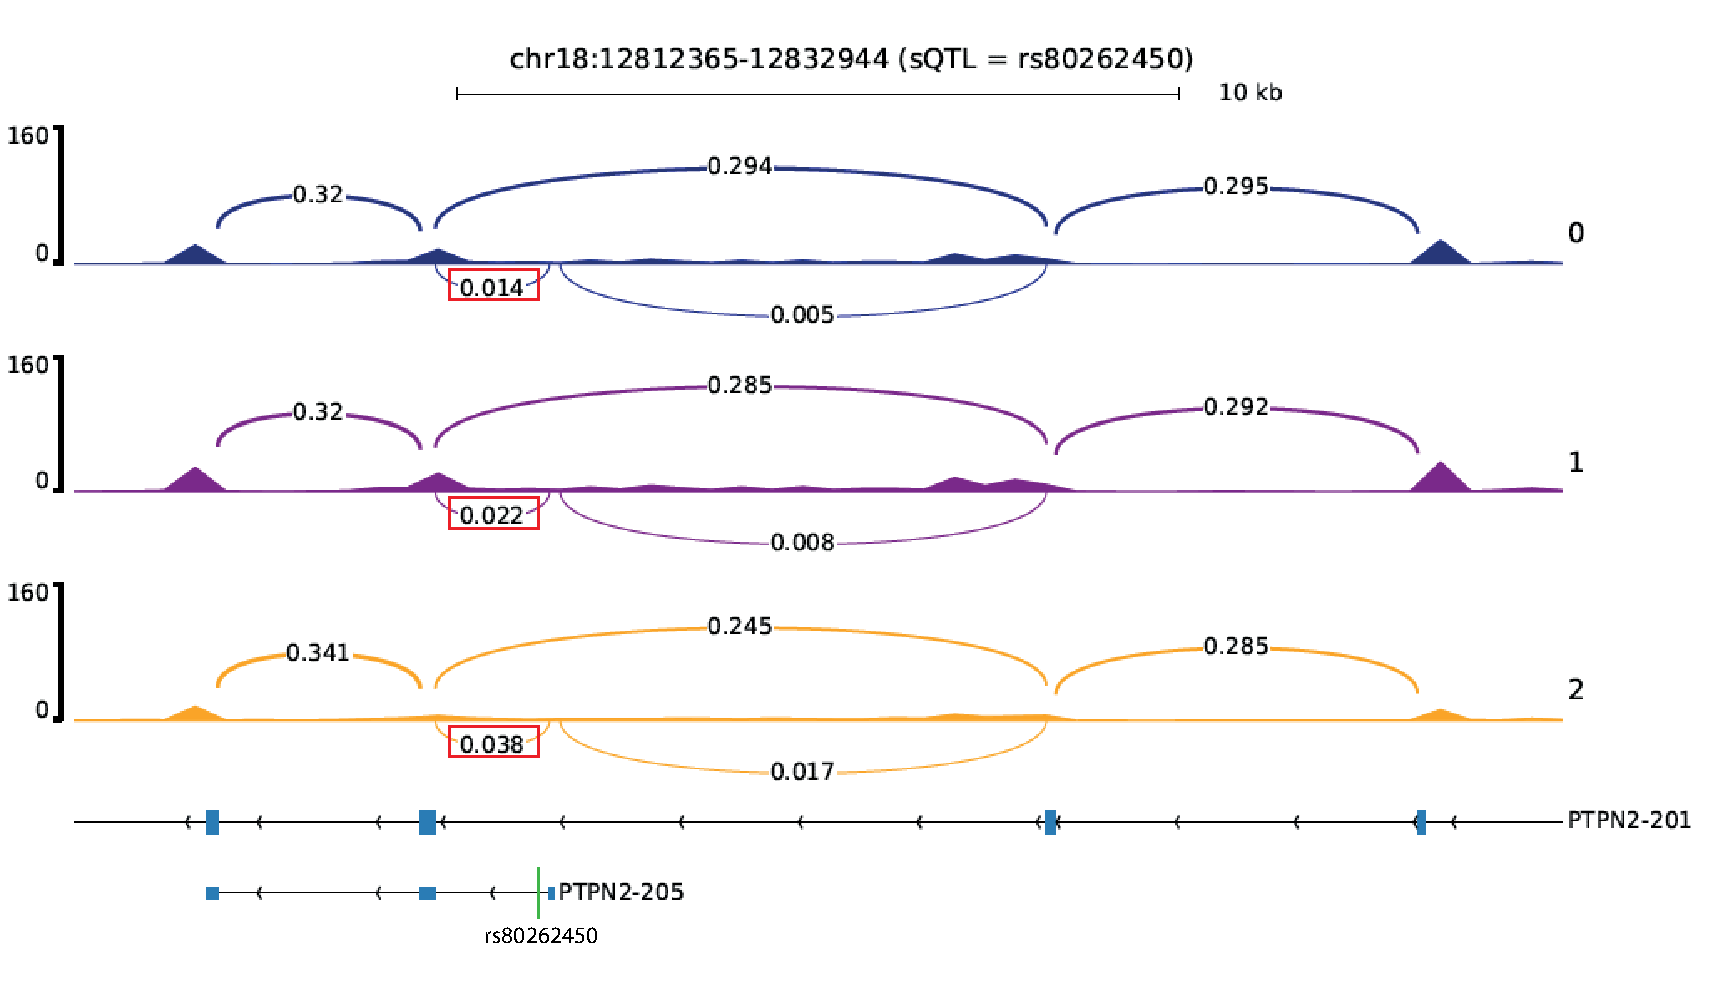
\includegraphics[width=0.9\textwidth]{ptpn2_sashimi}
  \caption[\textit{PTPN2} RNA-seq coverage plot]{RNA-seq coverage of the intron cluster where the \textit{PTPN2} sQTL effect is detected in sLPS\_6. Bars represent the number of reads and arcs represent the usage of different introns (only five splice junctions are shown for clarity and the colocalised sQTL splice junction is indicated in a red box). Canonical transcript \textit{PTPN2-201} and non-canonical transcript \textit{PTPN2-205} are shown underneath, with blue boxes representing introns and the position of rs80262450 on \textit{PTPN2-205} is shown as a green line.}
  \label{fig:ptpn2_sashimi}   
\end{figure}


The directions of effects of rs80626450 on intron usage and IBD risk suggest that an increase in the relative abundance of \textit{PTPN2-205} is associated with increased risk of IBD (for example the effect size in sLPS\_6=1.22  and IBD odds ratio=1.17, respectively). Given that mouse knock-out studies of \textit{PTPN2} suggest the gene plays an anti-inflammatory role in macrophages, I hypothesise that increased usage of \textit{PTPN2-205} attenuates the role of \textit{PTPN2} as a negative regulator of inflammation, which in turn increases the risk of IBD. 
\begin{figure}[H]
  \centering
  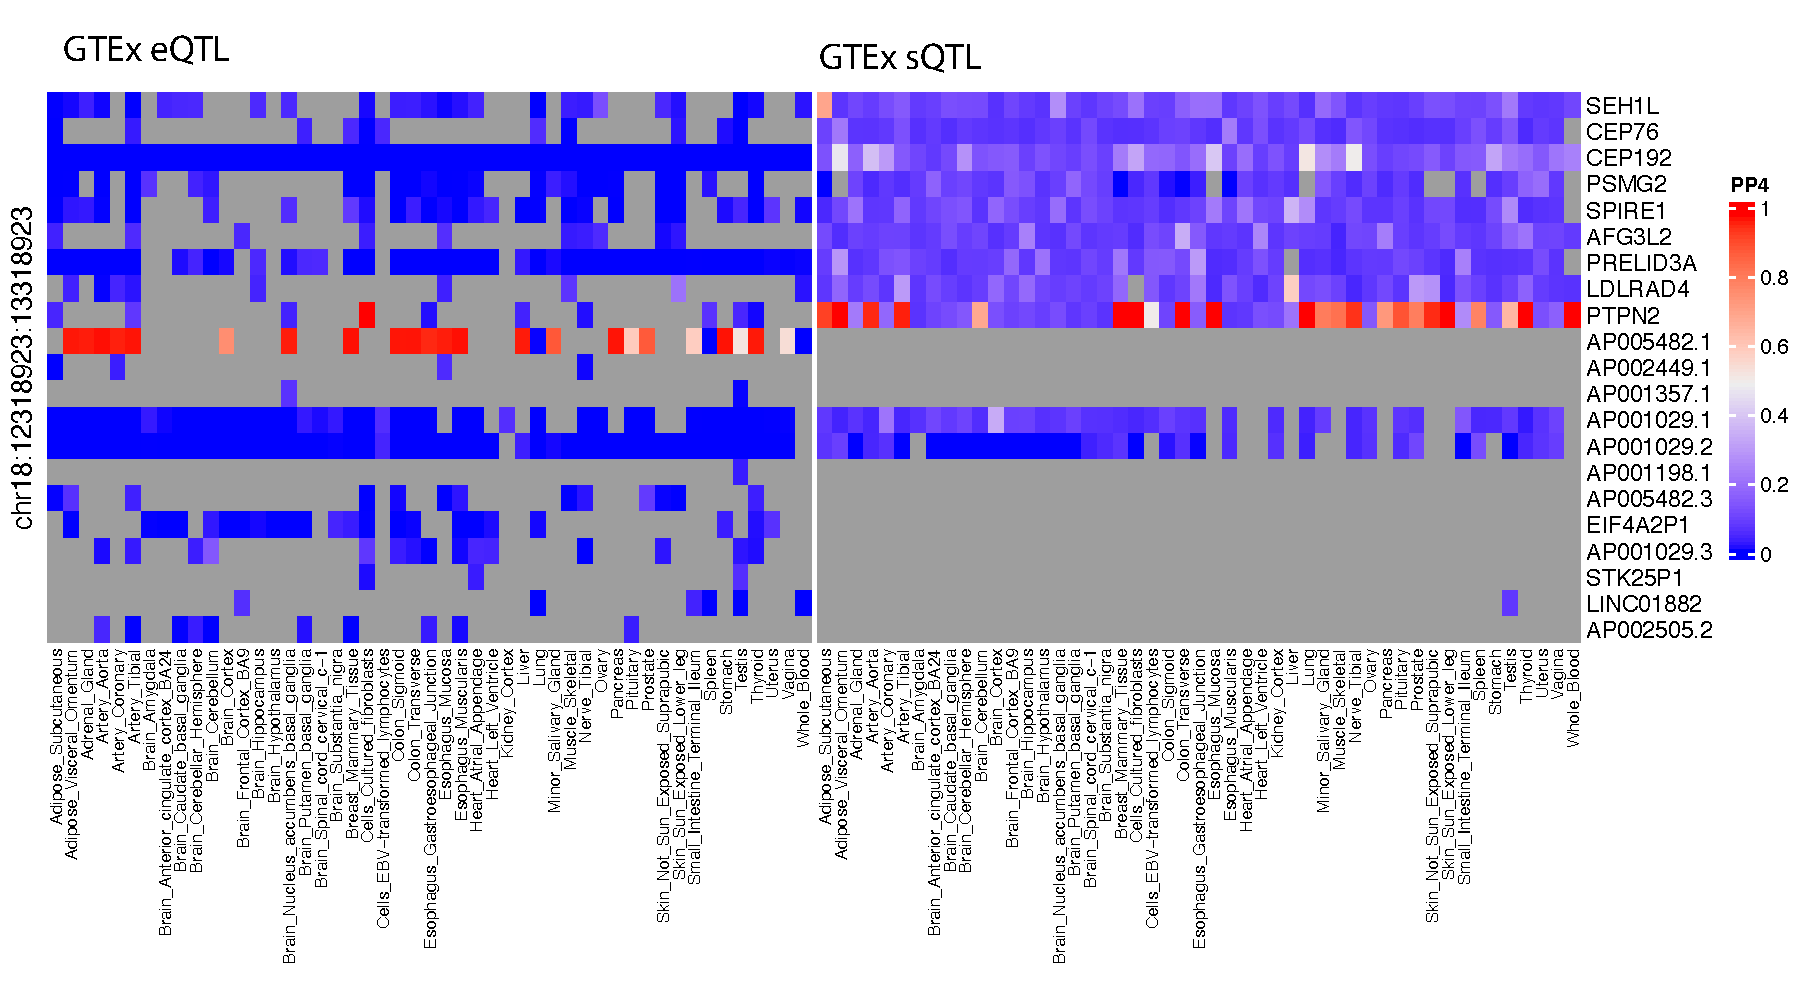
\includegraphics[width=1.0\textwidth]{ptpn2_gtex}
  \caption[Colocalisation of IBD-associated locus with \textit{PTPN2} QTLs in GTEx]{Heatmap of PP4 values for all genes in 18p21.11 (rows) and GTEx tissues (columns) split by type of QTL (eQTL on the left and sQTL on the right). For sQTLs, the intron with the highest PP4 value is shown. Although \textit{AP005482.1} shows strong colocalisation with GTEx eQTLs, it was removed from the current ENSEMBL release (November 2023).}
  \label{fig:ptpn2_gtex}   
\end{figure}
\subsection{sQTL colocalisations converge on dysregulated pathways in IMDs}
\begin{figure}
  \centering
  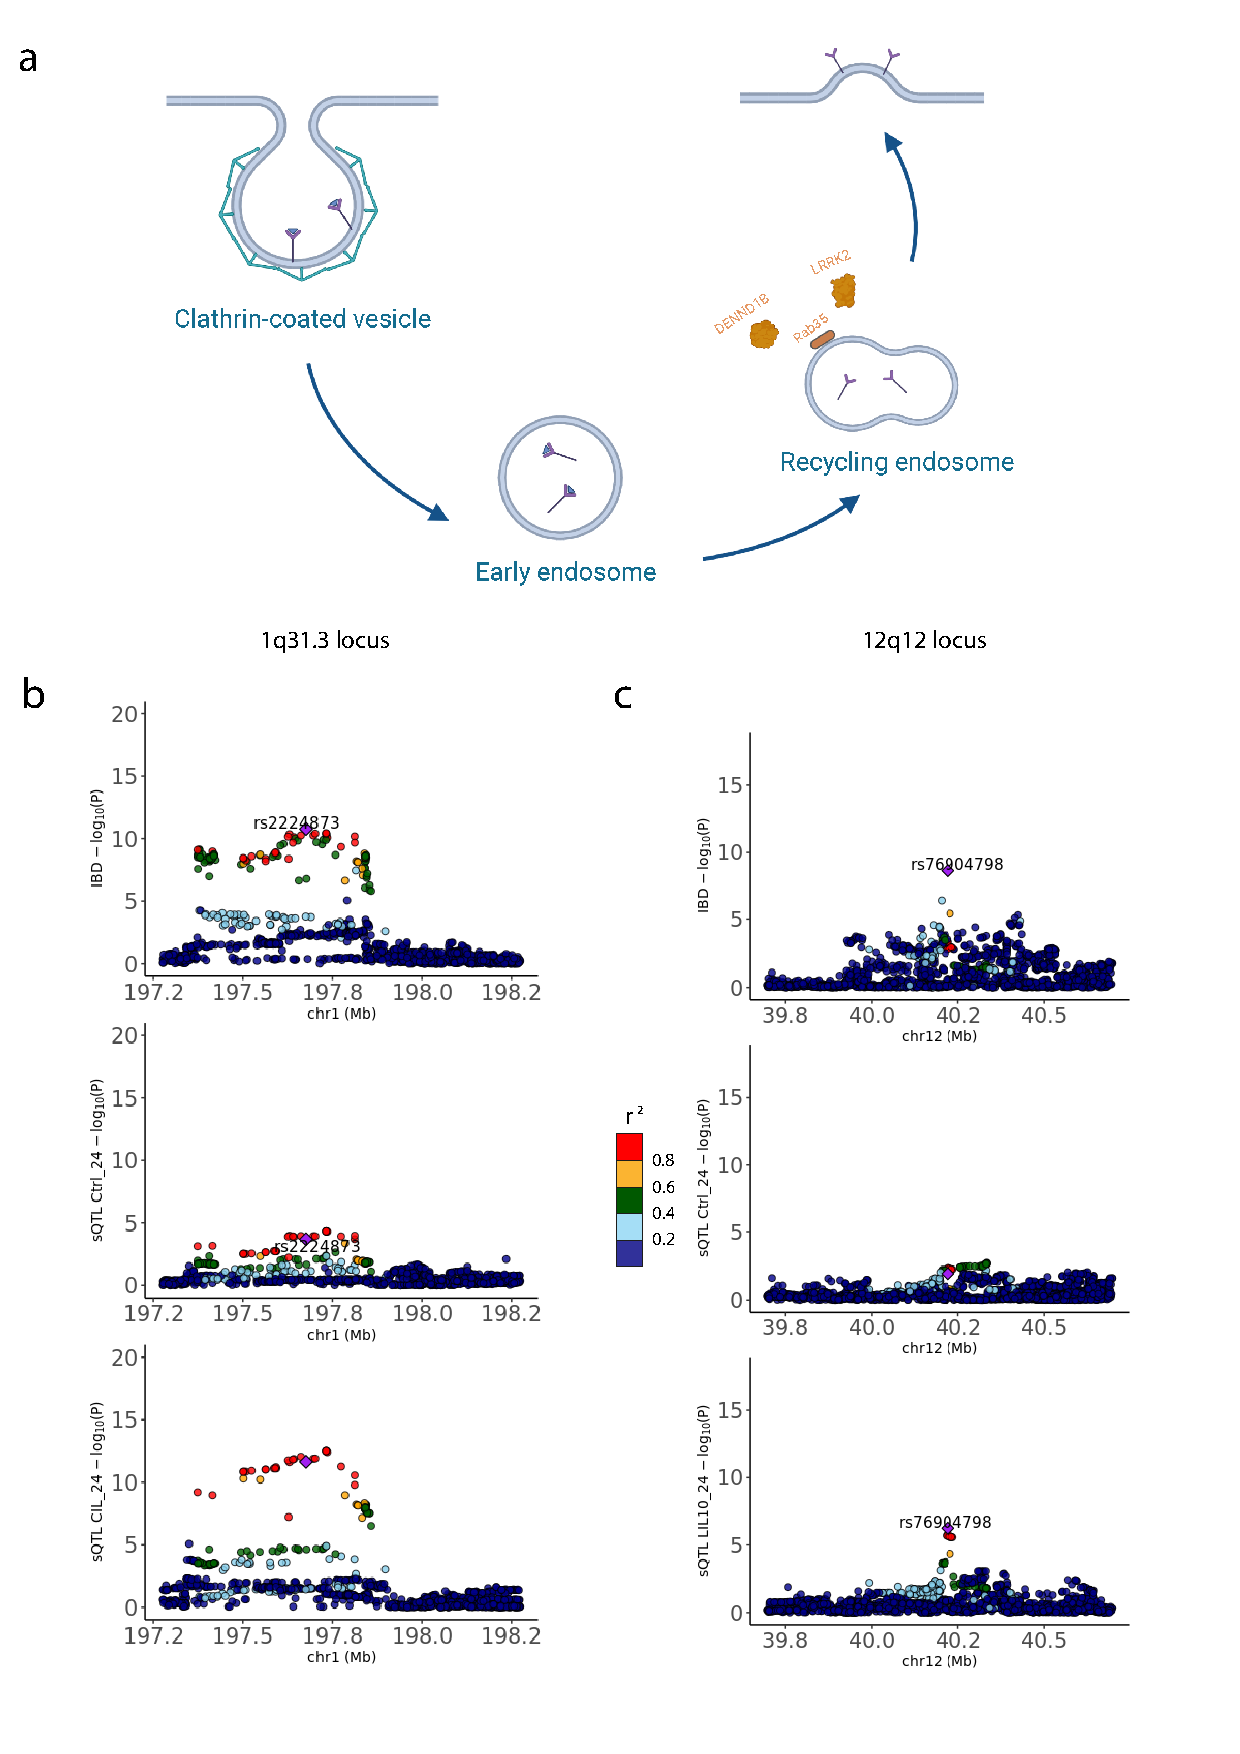
\includegraphics[width=0.8\textwidth]{dennd1b}
  \caption[Colocalisation of \textit{DENND1B} and \textit{LRRK2} sQTLs with IBD-associated loci]{(a) Diagram showing different stages of endocytosis and endosomal recycling. Rab35 and two of its interactors \textit{LRRK2} and \textit{DENND1B} are shown on a recycling endosome (created with BioRender.com). Regional Manhattan plots of the two IBD-associated loci are also shown (b) IBD-associated locus 1q31.1 and \textit{DENND1B} sQTL in naïve and stimulated macrophages (LIL10\_24) and (c) IBD-associated locus  12q12 and \textit{LRRK2} sQTL in naive and stimulated macrophages (CIL\_24). Panels b and c show high colocalisation evidence with the IBD-associated loci in the stimulated conditions, but not in the naïve conditions.}
  \label{fig:dennd1b}   
\end{figure}
IMD-sQTL colocalisations in disease-relevant cell types can reveal how genetic variation dysregulates biological pathways that enable the cell to perform its normal functions.
For example, I found that two IBD-associated loci colocalised with sQTL signals for genes that interact with the RAB GTPase Rab35. Rab GTPases are a diverse set of molecules that regulate different aspects of vesicle-mediated transport, with over 70 RAB GTPAses discovered so far \cite{Sigismund2021-cu}. RAB GTPases are activated by Guanine Exchange Factors (GEF), and subsequently recruit effector proteins, including proteins required for vesicle uncoating, movement, tethering and fusion, which enables cargo trafficking across cell compartments and membranes \cite{Yoneyama2005-ba}.\\

IBD-associated loci at 12q12 and 1q31.3 colocalise with \textit{LRRK2} and \textit{DENND1B} sQTLs in 5 and 21 conditions, respectively (PP4 $\geq$ 0.75; conditions with highest $PP_{4}$ are shown in Figure \ref{fig:dennd1b}). \textit{DENND1B} is a GEF that activates Rab35, while Rab35 was shown to be a bona fide substrate for \textit{LRRK2} \cite{Steger2016-yl,Bae2018-pu}, although the exact effect \textit{LRRK2} has on Rab35 is still debated \cite{Bae2018-pu,Bonet-Ponce2020-ri,Lee2021-ff}. Rab35 regulates endosomal recycling of both integrins and cadherins, effectively maintaining a balance between cell adhesion and cell migration. Moreover, evidence suggests that endosomal recycling in epithelial cells helps maintain apical and basolateral polarity, and that Rab35 plays a role in maintaining this polarity \cite{Mrozowska2016-lm,Kinoshita2020-yl}. The fact that both \textit{LRRK2} and \textit{DENND1B} interact with Rab35 suggests that endosomal recycling is frequently dysregulated by common IBD-associated variation. \\

Two \textit{DENND1B} splice junctions with different donor splice sites colocalise with the IBD-associated signal 1q31.3 (chr1:197,715,074-197,772,868 and chr1:197,715,074-197,735,586). The first splice junction is located in the coding sequence of the canonical transcript of \textit{DENND1B} (\textit{DENND1B-211}), while the second is part of the 5' untranslated region of another protein-coding transcript (\textit{DENND1B-201}). Lead sQTL SNPs for both transcripts have opposite directions of effect in different stimulation conditions where the colocalisations are detected (effect size and PP4 for \textit{DENND1B} splice junction chr1:197,715,074-197,772,868 is shown in Figure \ref{fig:lrrk2_dennd1b}) . This suggests that the effect of the risk-increasing allele may have opposite effects on relative transcript abundances is different environmental contexts. \\

Unlike \textit{DENND1B}, all \textit{LRRK2} sQTLs with high colocalisation probabilities (PP4 $\geq$ 0.75 in 5 conditions) had consistent directions of effects in the conditions where the colocalisation was detected. For example, the \textit{LRRK2} sQTL with the highest colocalisation probability was observed in LIL10\_24 (PP4=0.98), where the risk-increasing allele of the lead GWAS SNP (rs76904798) decreases the usage of an \textit{LRRK2} splice junction (chr12:40,316,403-40,319,988; beta=-0.75), and also increases the risk of IBD (beta=0.105). This indicates that decreased usage of this splice junction increases risk of IBD, and conversely that inclusion of this splice junction may have a protective effect against IBD (Figure \ref{fig:lrrk2_dennd1b}). \\

Although I demonstrate how \textit{LRRK2} and \textit{DENND1B} contribute to a dysregulated endosomal recycling in IBD in different environmental contexts, more research is still needed to understand the exact mechanisms by which the isoforms of these two genes affect such an important biological process in macrophages. \\
\begin{figure}[H]
  \centering
  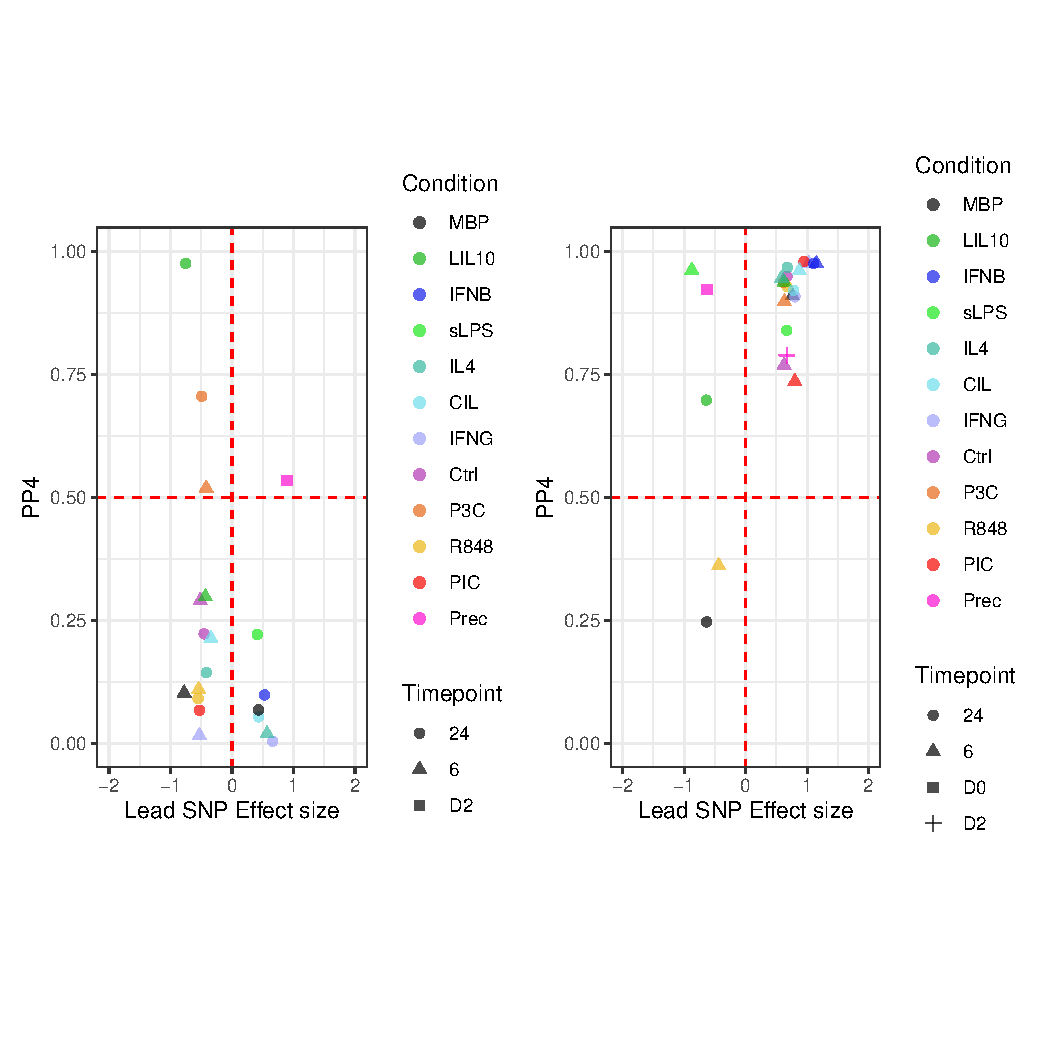
\includegraphics[width=1.0\textwidth]{lrrk2_dennd1b}
  \vspace{-70pt}
  \caption[Effect sizes and $PP_{4}$ values for \textit{LRRK2} and \textit{DENND1B}]{Effect sizes of the most significant SNP and colocalisation PP4 for the colocalised splice junctions of LRRK2 (left) and DENND1B (right).}
  \label{fig:lrrk2_dennd1b}   
\end{figure}


\newpage
\section{Discussion}

% \begin{itemize}
%   \item Differential splicing and response to pathogens - what we know - what needs to be done - cataolguing all isoforms
%   \item Why PTPN2 GTEx sQTL is colocalised - explain that they may contain macrophages
% \end{itemize}
In this work, I mapped splicing QTLs in iPSC-derived macrophages to understand how splicing is genetically controlled in macrophages in 24 conditions. I found thousands of genes with significant sQTL effects across our array of conditions, and that a considerable proportion of these genes have different effect sizes upon stimulation and were thus defined as response sQTLs.\\

The primary motivation behind several QTL mapping efforts is to understand the transcriptomic consequences of disease-associated genetic variation. Recently, Mostafavi et al. 2022 (ref 8) suggested that eQTL and GWAS studies are powered to discover systematically different types of variants, and that this may partially explain the limited colocalisation between eQTLs and GWAS risk loci. More than half of the IMD-associated risk loci that I tested likely share a single causal variant with either an eQTL or sQTL, with sQTLs solely contributing half of these loci, which clearly demonstrates the added value of sQTLs. This echoes previous work that showed the promise of sQTLs in closing the colocalisation gap \cite{Mu2021-ar,Kim-Hellmuth2020-gz,Liu2018-fh}. Mostafavi et al. (ref \cite{Mostafavi2022-tg}) proposed that systematic differences between GWAS and eQTL association signals are behind this colocalisation gap. Along the same lines, I attribute the large number of sQTL colocalisations to three important features of the discovered sQTLs that make them likely to colocalise with GWAS association signals. First, unlike eQTL variants, sQTL variants tend to be located closer to intron splice sites than gene TSS (Figure \ref{fig:intron_tss}), and are thus closer to intronic GWAS association signals that do not colocalise with eQTL signals. Indeed, 63.4\% of the lead SNPs in the GWAS loci that I tested were intronic variants. Second, sQTL signals largely do not colocalise with eQTL signals, suggesting that they are driven by distinct genetic associations (Figure \ref{fig:esqtl}). Third, I show that a considerable number of colocalisation events implicate unannotated introns that are lowly used across transcripts. These subtle changes in intron usage are unlikely to be reflected in overall levels of gene expression levels and may therefore remain undetected in eQTL studies. \\


Currently, it is unclear whether lowly-used splicing events are simply splicing errors \cite{Pickrell2010-lz,Melamud2009-my} or if they have functional consequences\cite{Wright2022-gp,Rotival2019-ic}. For example,  Pickrell et al. 2010 (ref \cite{Pickrell2010-lz}) interpreted the lack of evolutionary conservation around lowly-used splice sites as evidence that they are functionally irrelevant. This interpretation has been debated over the past decade \cite{Mazin2021-lb}. Here, I show that many of these lowly-used splice junctions may underpin disease-associated genetic effects on alternative splicing, and should not be considered noisy and functionally irrelevant. The \textit{PTPN2} example is particularly intriguing as the implicated splice junction falls within an Alu element, a class of Short Interspersed Nuclear Elements (SINE; Dfam E-value=$4.7\times10^{-98}$) that constitute 11\% of the human genome \cite{Deininger2011-cx}. RNA binding proteins normally repress the expression of newly-incorporated Alu elements, but decreased repression over long evolutionary periods provides a substrate for new functions \cite{Attig2016-mj,Singer2004-km}. The risk-increasing effect of the lowly-used \textit{PTPN2} splice junction could therefore represent a harmful evolutionary byproduct that attenuates the anti-inflammatory effect of \textit{PTPN2}. This remains to be validated by functional studies that profile the functional consequences of \textit{PTPN2} isoforms that contain this splice junction. With the recent success of RNA therapeutics such as splice-switching antisense oligonucleotides (ASO), it may be possible to “contain” these evolutionary side effects via therapeutic interventions that decrease the proportion of these lowly-used splice junctions \cite{Mercuri2018-pi,Roberts2020-rx}. This should provide incentive for the complex disease and transcriptomic community to understand and interrogate the functional consequences of the splicing events that underpin complex disease risk. \\

Although this dataset represents the largest resource for studying how alternative splicing is genetically controlled in iPSC-derived macrophages, I acknowledge two main limitations. First, although macrophages differentiated using MacroMap's experimental protocol have been shown to be transcriptionally similar to monocyte-derived macrophages \cite{Alasoo2018-pv}, they still do not capture the local environment of tissue-resident macrophages. This may limit the ability to understand the effect of local micro-environments on the transcriptome of macrophage \cite{Lavin2014-fb}. Second, intron usage ratios do not provide information about the relative abundance of full transcripts. For example, I demonstrated the potential effects of splicing events on the canonical transcripts of \textit{PTPN2}, but it is still unclear which transcripts these splicing events may have originated from. Fortunately, long-read sequencing and its algorithms for isoform quantification are becoming increasingly mature \cite{AlKhafaji2021-af,Amarasinghe2020-ci,Hu2021-bv}. I therefore expect that a more direct quantification of transcript usage will be attainable, and that it will make alternative splicing a more routine part of transcriptomic profiling studies. \\

In summary, these findings highlight an important role for alternative splicing in macrophage response to environmental cues, and that its dysregulation explains a large proportion of IMD-associated susceptibility loci. I anticipate that improved long-read sequencing technologies will facilitate whole isoform quantification in different cellular contexts, which will open the door for a better understanding of the role of different isoforms in innate immune response. Finally, I recommend that alternative splicing quantification should be an integral part of future QTL studies (including single cell studies), and that it will be increasingly relevant to understand the transcriptomic effects of disease-associated risk loci. 
\newpage






% %!TEX root = ../thesis.tex
%*******************************************************************************
%****************************** Third Chapter **********************************
%*******************************************************************************
\chapter{Genome-wide Meta-analysis of All-cause Perianal Disease}

% **************************** Define Graphics Path **************************
\ifpdf
    \graphicspath{{Chapter3/Figs/Raster/}{Chapter3/Figs/PDF/}{Chapter3/Figs/}}
\else
    \graphicspath{{Chapter3/Figs/Vector/}{Chapter3/Figs/}}
\fi

\section{Contributions}
UK Biobank phenotype and genotype data were obtained by Dr. Laura Fachal. Genotype quality control and principal component analysis were also performed by Dr. Laura Fachal. All the other analyses described here were performed by me. 
\section{Introduction}

In the previous chapter, I described the characteristics and genetic underpinning of perianal Crohn's disease. However, perianal disease (pAD) is not only associated with Crohn's disease. pAD encompasses a broader set of perianal manifestations such as perianal abscess, fissures, and fistulas.\\

Anal fissures are tears and/or ulcers in the perianal skin that cause sharp pain associated with defecation and rectal bleeding. They are classified as acute, lasting less than 6 weeks, or chronic. The etiology of anal fissures is still debated \cite{Beaty2016-yj}, but they are thought to be caused by trauma resulting from high anal canal pressure associated with constipation or diarrhea \cite{Mapel2014-wp}. Although recent population studies on the etiology of anal fissures are markedly lacking \cite{Mapel2014-wp}, a number of studies conducted between 1977 and 1983 found that chronic constipation accompanied fissures in only 25\% of patients while diarrhea accounted for less than 7\% \cite{Keighley2018-iy,McDonald1983-cs,Lock1977-go}. Anal fissures are conservatively treated with dietary and lifestyle modifications, analgesics, and fiber supplements \cite{nice_analfiss}. Anal fistula is a more serious perianal manifestation of pAD. An anal fistula is defined as an abormal communication between the anal canal and the perianal skin \cite{Sneider2013-qd}. It is characterised by pain, rectal discharge and bleeding, and causes significant lifestyle difficulties for patients \cite{Mei2019-ds}. The incidence of perianal fistulas varies per country, and a recent study in four European countries found that it ranges from 1.2 to 2.8 per 10,000 per year \cite{Zanotti2007-mb}, but its incidence is likely underestimated \cite{Eberspacher2022-sp}. Moreover, little is known about the pathophyiology of anal fistulas. Cryptograndualr fistulisation, a theory proposed by Parks in 1961 \cite{Parks1961-pe,Wlodarczyk2021-kh}, is the most accepted pathophysiological account for the origin of anal fistulas. Accoring to the cryptograndular theory, anal fistuls start as an inflammatory process in the proctodeal glands whose ducts extend to connect the perianal skin to the anal canal. Crohn's disease, tuberculosis \cite{Dudukgian2011-is}, ratiotherapy \cite{Johnston2003-jr}, sexually transmitted diseases \cite{Assi2014-at} and malignancy can contribute to these initial inflammatory process that resultin  anal fistula formation. However, over 90\% of cases remain idiopathic \cite{Simpson2012-gi}. Management of anal fistula depends on its type, extension, and underlying cause, but the end goal of all treatments is the complete drainage of abscess, and fistula healing while preserving anal sphincter function and continence. The management plan is typically decided based on a combined clinical, radiological and/or endoscopic assessment. Surgical options of fistula management include fistulectomy, the complete excision of the fistula tract, and fistuolotomy, in which the fistula is laid open and allowed to heal. Surgical procedures that preserve anal function such as fistolotomy with sphincter reconstruction have emerged in the last 30 years as a particularly effective method of treating anal fistulas, with lower incontinence and recurrence rates compared to fistulectomy \cite{Arroyo2012-qa,Jain2012-or}. \\

Despite recent advances in the management of pAD, little is known about the biological and pathophysiological processes that lead to anal fissure and fistula formation. Despite the overall consensus on the cryptoglandular theory, it is unclear if some individuals are at higher risk of developing pAD due to their genetic predisposition. Genome-wide association studies (GWAS) have significantly improved our understanding of the genetic factors underlying several complex diseases as well as the biological pathways implicated by disease-associated genetic variants. In the last 15 years, a typical GWAS required extensive coordination between researchers, clinicians and recruitment centres to construct case-control cohorts to study a particular disease or trait of interest. In recent years, efforts to build various national biobanks where genetic, and phenotypic data are available for hundreds of thousands of participants has significantly improved our ability to conduct GWAS of previously understudied diseases and traits. Their large sample sizes has made it possible to carry out GWAS of thousands of binary and contiunous traits and diseases, including relatively uncommon diseases. \\

Recruitment for the UK Biobank (UKBB) started in 2006, and has so far collected genotypic, biomarker and clinical data from electronic health records as well as blood and urine samples from over 500,000 participants \cite{ukbb_showcase}. The UKBB queries electronic health records for various types of data including deaths, cancer registrations, and hospital inpatient episodes. Electronic health records data are provided by external sources. Upon receipt of the data, a multi-step approach is followed, where received data is subjected to further pre-processing and quality checks to ensure its alignment with the UKBB data dictionary, and that it does not contain any ambiguities. The data is then consolidated into a central UKBB database and made available to researchers \cite{ukbb_ehr}.\\

FinnGen is another example of national biobanks that has made GWAS for various traits and diseases more feasible. FinnGen started in 2017 as a public-private partnership between several public Finnish institutions and thirteen international pharmaceutical companies \cite{finngen_forresearchers}. Importantly, FinnGen restricts access to individual-lvel data to approved researchers only. However, data from summary statistics from GWAS are conducted for  and made publicly available. In its latest release (data freeze 9), GWAS are available for over 2,200 binary endpoints from 377,277 individuals \cite{finngen_aboutdf9}. 

The UKBB and FinnGen use slightly different clinical coding systems to register clinical data. The UKBB uses the International Classification of Disease (ICD), a hierarchical clinical framework that organises clinical diagnoses in a tree-like structure. Different groups of diseases are organised in alphabetical chapters and particular diseases within each chapter are given a numeric value (e.g. chapter K contains digestive system disorders and K60 indicates anal fissure and fistula). Further detailed diagnosis subtypes are nested within each alphanumeric code up to four levels of resolution \cite{icd10_levels}. However, the UKBB only records up to two levels of resolution (e.g. K50.0 indicates Crohn's disease of the small intestine). FinnGen, on the other hand uses an expert-curated set of endpoints that are largely parallel to ICD-10 codes. These endpoints are designed to accommodate inclusion and exclusion criteria relevant for GWAS analyses \cite{finngen_endpoints}. Despite these differences, both resource are valuable for studying pAD. 

In this chapter, I will describe a pAD GWAS I performed in the UKBB to map pAD-associated genetic variants and I will describe the post-GWAS quality checks I carried out to ensure the validity of genome-wide significant loci. Additionally, I will outline how I used a similar FinnGen GWAS that I used as both a replication cohort, and as a constituent cohort in a meta-analysis I performed between the UKBB and FinnGen. Finally, I will describe two follow-up analyses that I performed to better understand the effects of pAD-associated variants on haemorrhoids, a closely-related disease, and identify effector genes at these loci.

\section{Methods}
\subsection{UKBB sample preparation and data access}
Hospital inpatient episode data and genotyped and imputed data were obtained under UK Biobank Application 45669. UKBB participants were genotyped using either UK Biobank Axiom Array \cite{ukbbaxiom_array} or the Affymetrix UK
BiLEVE Axiom array \cite{ukbbbelieve_array}. Sample processing, genotyping and quality control were performed at the UK Biobank, Affymetrix and the Wellcome Trust Centre for Human Genetics \cite{ukbb_sample_processing}. The imputation process has been previously described \cite{Bycroft2018-fj} and consists of imputing directly genotype data to the Haplotype Reference Consortium (HRC) and UK10K, resulting in 96 million variants. Imputed data was obtained as BGEN v1.2 files \cite{Band2018-tv}. 

\subsection{UKBB genotype quality control}
Genotyping array data from the UK Biobank dataset underwent quality control as part of the International IBD Genetics Consortium GWAS that is being undertaken in the laboratory, which resulted in 419,871 being retained. QC was performed using a combination of PLINK (v1.9 and v2) \cite{Purcell2007-mu}, bcftools (v1.16) \cite{Li2011-td}, and KING (v2.2.4) \cite{king-software}.  Variants that met the following criteria were excluded: 
\begin{itemize}
  \item Low call rate (<0.95 for variants with minor allele frequency (MAF) $>$ 0.01 or $<$ 0.98 for variants with MAF $\leq$ 0.01).
  \item Significant difference in genotype call rate (P-value $< 10^{-4}$) between IBD cases and controls.
  \item Large allele frequency (AF) differences between UKBB and Gnomad (Non-Finnish Europeans), or TOPMed (global) using the following formula: $\frac{(P_{1}-P_{0})^{2}}{(P_{1}+P_{0})(2-P_{1}-P_{0})} > \epsilon$, where $\epsilon=0.025$ or $0.125$, for Gnomad and TOPmed respectively,  $P_{0}$ is the minor allele frequency (MAF) in Gnomad or TOPMed and $P_{1}$ is the UKBB MAF. 
\end{itemize}

Genotypic principal components (PC) were estimated for all participants, using a set of genotyped variants that were also available in the 1000 Genomes Project (100GP; excluding variants associated with IBD susceptibility; P-value < $10^{-4}$, and variants in long LD regions (as defined in \cite{plink_high_ld}). This final list was pruned with the following parameters: window size = 50 kbp; step size = 5; $R^{2}$ = 0.2. PCs were then projected to 1000GP PCs. Samples within the European ancestry group were retained for the subsequent analyses. 



\subsection{UKBB GWAS using REGENIE}
All genome-wide association analyses were performed using REGENIE v3.2.5 \cite{Mbatchou2021-qm} following a 2-step procedure. Briefly, in step 1, a whole-genome regression model is fitted using a subset of high-quality genome-wide variants in order to estimate a set of genome-wide predictors that capture a large fraction of phenotypic variance. These predictors are then used as covariates in step 2 where a larger set of variants of interest are tested for association.
I used post-QC genotyped variants in step 1 as recommended by REGENIE documentation (N=419,871), and both genotyped and imputed variants in step 2, testing all autosomal chromosomes (N=9,705,089). Additionally, I enabled a Firth correction of effect sizes for all variants with P-value < 0.01 in order to account for the case-control imbalance in the pAD cohort (\Verb+--firth --approx --pThresh 0.01+). The Firth test corrects biased effect sizes and P-values obtained from highly unbalanced case-control designs, where such an imbalance causes unreliable P-values, inflating Type I error. Approximate Firth logistic regression is a variant of the Firth test that is implemented in REGENIE, which is more computationally tractable. 

\subsection{LD calculation from 1000GP}
Reference LD panels obtained from the 1000 Genomes Project High Coverage project were used for different types of analysis, including genome-wide loci identification using LD clumping, and post-GWAS checks to study the relationship between LD and association strength at genome-wide significant loci. $R^{2}$ values were calculated between the index variant and all variants in each locus. I downloaded VCFs from the 1000GP high coverage and used PLINK v1.9 to compute LD between all variants and the index variant at each locus. For each GWAS check I used individuals unrelated individuals assigned to the relevant reference population: NFE for UKBB and FE for Finngen, and GBR for the follow-up quality check on UKBB index variant 6:31113288\_T\_C (N=426, 99 and 90 respectively). Only one sample was retained from the trios found in 1000GP. Relevant samples were included in the LD calculation using the following PLINK command:
\begin{verbatim}
  plink --r2 --keep EUR.samples --ld-window-r2 0 
\end{verbatim}

\subsection{Defining genome-wide significant loci in UKBB}
I defined genome-wide significant loci from the UKBB pAD GWAS summary statistics using PLINK v1.9 via a clumping procedure. Briefly, clumping chooses the most significant variant in a user-defined window to represent each locus (termed index variant). It then proceeds to define the locus boundaries by clumping neighbouring correlated variants. Specifically, any variants within the predefined window that are correlated with the index variant are considered to belong to the same locus represented by the index variant (i.e. variants in high LD). I used VCFs downloaded from the 1000GP, which I used compute LD, and set a maximum P-value of $5\times10^{-8}$ for defining a genome-wide significant locus, with default values for the rest of the parameters: variants with $R^{2}$ < 0.5, variants outside a window of 250 kbp, or variants that have a P-value > 0.01 are not clumped with the index variant.
\begin{verbatim}
  plink --clump-p1 0.00000005 --clump-r2 0.50 --clump-kb 250 
  --clump-p2 0.01
\end{verbatim}

PLINK outputs each locus' index variant along with any variants that meet the clumping criteria outlined above. I then defined each locus' boundaries by sorting the clumped variants within each locus according to their genomic location: the most downstream variant defined the 5' boundary and the most upstream variant defined the 3' boundary. 

\subsection{Finngen summary statistics preprocessing}
Publicly available FinnGen GWAS summary statistics (data freeze 7) were downloaded from the FinnGen results website \Verb+finngen.fi/en/access_results+. Similar to UKBB, variants with MAF < 0.01 were removed, but imputation quality information were not available, so I was not able to filter out variants with low imputation quality. The association summary statistics showed evidence of moderate genomic inflation ($\lambda_{GC}$=1.089). Using LD clumping with a 1000GP-derived FE LD reference panel, I identified three genome-wide significant loci. 

\subsection{Meta-analysis of UKBB and Finngen}
I used METAL to perform the meta-analysis between UKBB and FinnGen GWAS summary statistics.  METAL can perform fixed-effects meta-analysis using one of two different well-established schemes: P-values and effective sample size, or effect sizes and standard errors. The P-value scheme is implemented to enable meta-analysis of GWAS summary statistics that do not report the effect allele, while the effect sizes scheme can be used when each variant's effect size and effect allele are reported. Both my UKBB analysis and FinnGen's summary statistics report the effect allele, so I used the effect size scheme of METAL (\Verb+SCHEME STDERR+). \\

Moreover, METAL automatically aligns any variants that may be flipped between the meta-analysed summary statistics. METAL also enables filtering of variants to be meta-analysed based on their allele frequencies, which was not necessary since I previously filter out variants with MAF < 0.01 in each summary statistics file. Finally, given the differences, allele frequencies, and potential subpopulation stratification between the FinnGen and UKBB GWAS, I enabled a METAL option to correct genomic inflation before performing the meta-analysis (\Verb+GENOMICCONTROL ON+) as recommended in METAL's documentation website. There was no evidence of genomic inflation in the meta-analysed summary statistics ($\lambda_{GC}$=1.024).\\

For each variant, METAL outputs the effect allele, meta-analysed effect size, standard error, and P-values. After performing meta-analyses, it is important to compare the effect sizes between the meta-analysed cohorts. Comparison of both the direction and magnitude of effect sizes gives an indication on how similar the estimated effects of meta-analysed genetic variants are. To formally test this, METAL uses Cochran's Q test to test for effect size heterogeneity. Cochran's Q test asseses two or more effect size estimates and their corresponding standard errors and reports a $\chi^{2}$ statistic that quantifies the deviation from the null hypothesis that the meta-analysed effect sizes are similar. Depending on the number of meta-analysed studies (in this case 2), a P-value is derived from a theoretical $\chi^{2}$ distribution with $N-1$ degrees of freedom, where N is the number of meta-analysed studies (heterogeneity of effect P-value $P_{het}$). I used $P_{het}$ to test if index variants at genome-wide significant loci demonstrate heterogeity of effect size between the two cohorts. To account for multiple index variants being tested, I set a Bonferroni-coorected P-value threshold for rejecting the null hypothesis that the effect sizes are significantly different between the two studies (P-value < $\frac{0.05}{k}$, where $k$ is the number index variants tested).


\subsection{Defining genome-wide significant loci in the UKBB/FinnGen meta-analysis}
Meta-analysis associations are derived from two different populations with different LD structures (NFE and FE). 
For these associations, a  representative LD reference panel that captures the true underlying LD pattern in the meta-analysis is not easy to obtain because LD will be dependent on the contribution of each population to the association signal. However, an LD reference panel is needed both to define genome-wide significant loci based on LD clumping, but also to perform post-GWAS checks. To this end, I identified genome-wide significant loci similar to UKBB and FinnGen, except that I performed LD clumping with both FE and NFE in 1000GP as a reference panel. Both LD clumping procedures identified the same 18 genome-wide significant loci, but their boundaries differed slighly. I defined consensus loci boundaries as the union of loci boundaries defined by NFE- and FE-based LD clumping. \\

\subsection{Quality control of meta-analysis genome-wide significant loci}
For all 18 genome-wide significant loci identified via the initial LD clumping procedure, I investigated the LD friends of each index variant. Specifically, for each index variant, I checked if the P-values of its LD friends decay with their LD values with the index friends. In a meta-analysis between different subpopulations, it is important to ensure that P-values match expectation under LD  in all the constituent cohorts. I therefore computed the correlation between P-values and LD in both NFE and FE for all 18 loci. Six loci showed that the index variant had no LD friends in NFE or FE, or that there was weak or non-existent correlation beween P-values and LD of the index variant's LD friends in NFE or FE (Pearson correlation coefficient between $-log_{10}(P)$ adn ($R^{2}$ $\rho$ < 0.2). I removed these six loci from all downstream analysis.









\subsection{Genetic correlation analysis}
Genetic correlation analysis is commonly employed to understand the genetic similarities between two phenotypes or diseases of interest. I used genetic correlation to understand the overall genetic similarity between pAD and haemorrhoids. Linkage disequillibrium score regression is a common method to compute genome-wide genetic correlation,(LDSC \cite{Bulik-Sullivan2015-fk}) as it leverages association summary statistics between a pair of traits to compute a genetic correlation estimate ($r_{g}$). The availability of GWAS summary statistics for large numbers of traits and diseases makes genetic correlation a feasible exploratory analysis to discover genetic similarities between traits.\\

The fundamental concept of LDSC is that there is a linear relationship between the Z-score product ($z_{1}z_{2}$) and the LD score of SNPs, where LD score is defined as the sum of $R^{2}$ values for all SNP in a pre-defined windown (the default is 1 cM) \cite{Bulik-Sullivan2015-ts}. The rationale behind this relationship is that SNPs with a higher LD score are more likely to tag the causal variant at each locus, and will therefore have a larger $z_{1}z_{2}$ value. Regressing the LD score for all SNPs can give an estimate of the overall genetic covariance between two traits.Specifically, the regression slope quantifies the gentic covariance, which can then be normalised by the sample sizes of the two traits and the number of SNPs to obtain a genetic correlation estimate between the two traits ($r_{g}$).\\

The accuracy of $r_{g}$ rests on the assumption that the GWAS populations match the LD scores population. By default, LD scores are provided by LDSC, which are computed from the HapMap3 European-ancestry reference panel \cite{hapmap}. It is also important to note that although $r_{g}$ is a genome-wide measure, its computation is based on a predefined set of SNPs. The estimation of $r_{g}$ is based on a set of high-quality common SNPs in HapMap3, which is also provided by LDSC (MAF $\geq$ 0.05; N=1,217,312).

\subsubsection{Genetic correlation between pAD and haemorrhoids}
I used LDSC to compute $r_{g}$ between my pAD meta-analysis and two haemorrhoids GWASes (Zheng et al. 2021 \cite{Zheng2021-ss} and the Pan-UKBB GWAS: \Verb+pan.ukbb.broadinstitute.org/+). I downloaded the Zheng et al. 2021 summary statistics via the GWAS catalogue website (study accession: GCST90014033; $N_{cases}$=218,920; $N_{controls}$=725,213). Since the Pan-UKBB performed the haemorrhoids GWAS using different ancestries, I used the summary statistics from the European-ancestry GWAS only (ICD-10 code: I84; $N_{cases}$=26,348; $N_{controls}$=394,183). \\

After downloading the two haemorrhoids summary statistics, I preprocessed both of them using the LDSC script \Verb+munge_sumstats.py+. The script filters the SNPs and aligns their alleles to the HapMap3 SNP list using the flag \Verb+--merge_alleles hm3.snplist+. This script also takes as input a signed summary statistic column which I provided using the flag \Verb+--signed-sumstats effect_size,0+, where the first argument specifies the column name (effect size column) and the second argument specifies the expected value of the signed summary statistic. Each of the two "munged" summary statistics files were then provided as input to the \Verb+ldsc.py --rg+, along with the pAD summary statistics file, and $r_{g}$ is then computed between pAD and each of the two haemorrhoids GWASes. 


\subsection{Colocalisation analysis}
In order to link the meta-analysis genome-wide significant loci to effector genes, I performed statistical colocalisation with a set of expression and splicing QTLs from the Genotype Excpression Project (GTEx v8). Colocalisation analysis is a statistical approach that uses two summary statistics from two association studies in order to make an inference whether the two association signal are likely to be driven by a shared causal variant. A fundamental assumption of colocalisation is that a single causal variant underlies both association signals under comparison. Under this assumption, five different hypothesis regarding the relationship between the two association signals are tested:
\begin{itemize}
  \item $H_{0}$: none of the two signals are associated with their corresponding traits
  \item $H_{1}$: only the first signal is associated with its corresponding trait
  \item $H_{2}$: only the second signal is associated with it corresponding trait
  \item $H_{3}$: the two signals are associated with their corresponding traits, with different underlying genetic variants
  \item $H_{4}$: the two signals are associated with their corresponding traits, and share a single underlying genetic variant.
\end{itemize}
Certainty about each of these hypotheses is quantified as a posterior probability. Therefore, colocalisation analysis outputs four different posterior probabilities: $PP_{0}$, $PP_{1}$, $PP_{2}$, $PP_{3}$, and $PP_{4}$. Statistical colocalisation is implemented in the R package \Verb+coloc v5.1.2+.

To maximise the ability of \Verb+coloc+ to identify effector genes, I downloaded summary statistics from GTEx v8, a large compendium of expression and splicing quantitative trait loci (eQTLs and sQTLs) mapped from RNA-seq samples obtained from 49 human tissues, ranging in sample sizes from 73-706 individuals. eQTLs and sQTLs were mapped in a 1mbp window around the transcript start site (TSS) of each gene (cis-eQTLs and cis-sQTLs) using genotyped or imputed variants with MAF $\geq$ 0.01.

Within each of the meta-analysis genome-wide significant loci, I identified a list of genes and splice junctions for eQTL and sQTL colocalisation, respectively. To achieve this, for each locus I defined a 1 mbp window around the index variant at each locus, and created a set of genes and splice junction whose respective TSS is located within this window. Next, I performed colocalisation analysis between the meta-analysis summary statistics and each gene's or splice junction's summary statistics. I used the \Verb+coloc.abf()+, which takes as input effect sizes and standard errors of each variant from the meta-analysis and gene or splice junction being tested. Importantly, \Verb+coloc.abf()+ does not require the effect sizes to be aligned to the same effect allele, as the Bayes Factor calculation implemented in \Verb+coloc+ relies on the $Z^{2}$ statistic to compute the posterior probabilities. Finally, I used the default priors implemented in \Verb+coloc.abf()+: prior probability a SNP is associated with pAD=$10^{-4}$, prior probability a SNP is associated with the eQTL/sQTL=$10^{-4}$.

\begin{table}[H]

  \caption{Number of eQTL and sQTL genes tested for colocalisation across all GTEx v8 tissues. All genes and splice junctions in a 1mbp around each index variant were tested.}
  \centering
  \begin{tabular}[t]{|l|r|r|}
  \hline
  Index variant & Number of tested eQTL genes & Number of tested sQTL genes\\
  \hline
  3:53034026\_C\_T & 41 & 18\\
  \hline
  5:64868326\_TTTC\_T & 13 & 4\\
  \hline
  6:1775202\_G\_A & 12 & 5\\
  \hline
  6:31121854\_C\_T & 89 & 45\\
  \hline
  6:31253340\_T\_C & 98 & 50\\
  \hline
  6:133260944\_G\_A & 18 & 7\\
  \hline
  7:2524404\_G\_A & 21 & 13\\
  \hline
  8:70735125\_A\_G & 15 & 6\\
  \hline
  8:70993166\_AAGTT\_A & 10 & 6\\
  \hline
  9:22124505\_A\_T & 19 & 5\\
  \hline
  11:10356352\_C\_A & 20 & 11\\
  \hline
  12:114235969\_T\_C & 18 & 10\\
  \hline
  \end{tabular}
  \end{table}



\section{Results}


\subsection{Defining pAD case control cohorts}
% With every inpatient visit, patients receive a primary and secondary diagnosis. These diagnoses are recorded using a hierarchical clinical diagnosis framework known as The International Classification of Diseases (ICD) \cite{Hirsch2016-mw}. ICD is a hierarchical framework whereby each medical diagnosis is given an alphanumeric code, and all sub-classifications of any given diagnosis are nested within it. For example, K50 codes for Crohn's disease, while K50.1 codes for Crohn's disease in the large intestine. In this chapter, I will refer to the main ICD codes as "level 1 codes" and their sub-classifications "level 2 codes". The level 1 code for perianal involvement is K60 (K60: Fissure and fistula of the anal and rectal regions)

% To understand the genetic architecture of perianal involvement in the general population, I performed a GWAS analysis between all-cause peri-anal disease (pAD) and healthy individuals in the UKBB. 

\subsubsection{Control exclusion criteria}
To avoid contamination of controls with lower digestive tract disorders that may be true pAD cases that were incorrectly diagnosed, I applied a set of control exclusion criteria. Specifically, I excluded from the control set any individuals who had an ICD-10 hospital diagnosis of K55-K64 and their corresponding ICD-9 codes as demonstrated in Table \ref{table:ukbb_ctrl_excl_criteria}; collectively grouped as "Other diseases of intestines" in ICD-10). These ICD codes cover disorders with symptoms that may resemble pAD symptoms upon presentation, and include ano-rectal bleeding (K55 vascular disorders of the intestine, K57 diverticular disease of intestine and K64 Haemorrhoids and perianal venous thrombosis), or a change in bowel habits (K56 Paralytic ileus and K58 Irritable bowel syndrome), perianal fistula or abscess (K60 fissure and fistula of the anal region and K61 abscess of the anal and rectal region), any ano-rectal abnormalities (K62), or proximal fistulas or abscesses (K63). In total, I excluded 133,398 from 481,756 pAD controls (27.7\%); per-code numbers in Table \ref{table:ukbb_level2_nums}).

\subsubsection{Case inclusion criteria}
To define the case cohort, I identified all individuals with ICD-10 and ICD-9 codes K60
and 565 as cases. In total, 5,257 UKBB participants had at least a single visit where they received either a primary or secondary pAD diagnosis or its corresponding ICD-9 code ("anal fissure and fistula"; 565). Six level-2 codes are nested within K60, representing two broad categories of pAD: fissures and fistulas. Three codes are used for acute and chronic fissures and three codes for acute and chronic fistulas. 92\% of patients (4,858) presented with either K60.1, K60.2 or K60.3 ("chronic anal fissure", "anal fissure, unspecified" and "anal fistula", respectively; Table \ref{table:ukbb_level2_nums}).



\begin{table}[H]
  \centering
  \caption{Number of UKB participant with with a primary or secondary diagnosis for each K60 level 2 code. K60.0=Acute Anal Fissure; K60.1=Chronic Anal Fissure; K60.2=Anal Fissure; unspecified; K60.3=Anal Fistula; K60.4=Rectal Fistula; K60.5= Anorectal Fistula}
  \label{table:ukbb_level2_nums}
  \begin{tabular}{|l|l|l|l|l|l|l|}
  \hline
  ICD-10 code           & K60.0  & K60.1  & K60.2  & K60.3 & K60.4 & K60.5\\ \hline
  Number of individuals & 144                      & 788                        & 2,624                           & 1,954              & 76                   & 122                     \\ \hline
  \end{tabular}
  \end{table}




\begin{table}[H]
  \caption{pAD control set exclusion criteria. All ICD-10 codes had corresponding ICD-9 codes except K56 K62 and K63. For those, ICD-9 codes were obtained manually by inspecting level-2 ICD-10 codes and searching for their corresponding level-2 ICD-9 codes.}
  \label{table:ukbb_ctrl_excl_criteria}
  \begin{tabular}{|p{0.1\linewidth}|p{0.2\linewidth}|p{0.2\linewidth}|p{0.3\linewidth}|p{0.1\linewidth}|}
  \hline
  ICD-10 code & ICD-10 meaning                                            & ICD-9 code                          & ICD-9 meaning     & N                                                                                                                                                          \\ \hline
  K55         & Vascular disorders of intestine                           & 557                                 & Vascular insufficiency of intestine       & 2923                                                                                                                                  \\ \hline
  K56         & Paralytic ileus and intestinal obstruction without hernia & 5600, 5601, 5602, 5603, 5608A, 5608, 5609 & Intussusception, Paralytic ileus, Volvulus, Impaction of intestine,Other specified intestinal obstruction, Unspecified intestinal obstruction & 9257                              \\ \hline
  K57         & Diverticular disease of intestine                         & 562                                 & Diverticula of intestine              &     61519                                                                                                                                  \\ \hline
  K58         & Irritable bowel syndrome                                  & 5641                                & Irritable bowel syndrome          & 12418                                                                                                                                          \\ \hline
  K59         & Other functional intestinal disorders                     & 564                                 & Functional digestive disorders not elsewhere classified      & 30087                                                                                                               \\ \hline
  K60         & Fissure and fistula of anal and rectal regions            & 565                                 & Anal fissure and fistula     & 5079                                                                                                                                               \\ \hline
  K61         & Abscess of anal and rectal regions                        & 566                                 & Abscess of anal and rectal regions              &     2178                                                                                                                        \\ \hline
  K62         & Other diseases of anus and rectum                         & 5690, 5691, 5692, 5693, 5694            & Anal and rectal polyp, Rectal prolapse, Stenosis of rectum and anus, Hemorrhage of rectum and anus, Other specified disorders of rectum and anus            & 39191                \\ \hline
  K63         & Other diseases of intestine                               & 5695, 5696, 5697, 5698, 5699            & Abscess of intestine, Colostomy and enterostomy complications, Complications of intestinal pouch, Other specified disorders of intestine, Unspecified disorder of intestine & 33307 \\ \hline
  K64         & Hemorrhoids and perianal venous thrombosis                & 455                                 & Hemorrhoids & 19060\\ \hline

  \end{tabular}
  \end{table}
  \subsection{pAD cases are enriched in multiple disorders compared to pAD controls}\label{section:pheno_enrich}
  The availability of a large number of clinical diagnoses and phenotypes for UKBB participants enables a thorough characterisation of the pAD case cohort. I aimed to understand the cohort composition and identify which ICD-10 codes are enriched in cases versus controls. For each ICD-10 code, I compared the prevalence in pAD cases versus controls, and I formally tested the enrichment of 1,693 codes using Fisher's exact test. \\

In total, 198 codes were significantly enriched (Fisher's exact  P-value < $3\times10^{-5}$; top 20 enriched ICD-10 codes are shown in \ref{fig:pheno_enrich}). Overall, the enrichment odds ratio was higher than expected (median odds ratio=1.36), likely as a consequence of sampling a disease cohort within a healthy population cohort. Within digestive systems disorders, ICD-10 code K61 (abscess of anal and rectal regions), followed by K50 (Crohn's disease) were the most significantly enriched (odds ratio=57 and 7.9 respectively). This is expected as many perianal fistulas start as abscess of the perianal region that later extends to form a fistula connecting the anorectal canal to the perianal skin \cite{abscess_fist}, and perianal fissures and fistulas are known subphenotypes of CD \cite{Marzo2015-wf}. Other examples indlude K57 (Diverticular disease of the intestine; odds ratio=2.1; P-value=$1.2\times10^{-87}$), which is also a known cause of pAD \cite{div_pad}. Among non-digestive codes, haemorrhoids (I84) was the most significantly enriched diagnosis (P-value=$6\times10^{-98}$; 38\% in pAD cases versus 6\% in controls; odds ratio=9.7). This enrichment could indicate a shared pathogenesis between haemorrhoids and pAD. However, it could also be due to a higher likelihood of diagnosing haemorrhoids in patients with more serious ano-rectal disorders such as pAD, compared to the general population where haemorrhoids patients with no other ano-rectal manifestations are less likely to seek medical advice, and may therefore remain undiagnosed. \\

    %To understand which groups of disorders were most enriched in pAD cases, I counted the number of enriched disorders within each ICD-10 code categry. I found that five groups had > 10 enriched ICD codes. The largest number of enriched codes belonged to: "Symptoms, signs and abnormal clinical and laboratory findings, not elsewhere classified (R00-R99)" (36 codes), followed by "Diseases of the digestive system (K00-K95)" (34 codes), "Diseases of the genitourinary system (N00-N99)" (22 codes), "Diseases of the musculoskeletal system and connective tissue (M00-M99)" (20 codes), and "Diseases of the skin and subcutaneous tissue (L00-L99)" (15 codes), "Diseases of the circulatory system (I00-I99)" (13 codes).\\
% However, not all enrichments were expected. For example, pAD cases were 1.6 more likely to be diagnosed with gonorthrosis, a gradual erosion of the knee cartialge (P-value=$1.3\times10^{-22}$; odds ratio=1.6; prevalence in pAD cases is 12\% versus 8\% in controls). A clinical report has previously described chronic arthritis as an "unusual complication" of poorly treated anal fistulas. However, it remains to be answered if such higher prevalence in UKBB can be attributed to poor management or complications, or if it suggests a musculoskeletal or connective tissue pathology underlying fissures and fistulas. 



\begin{figure}[H] 
  \centering    
  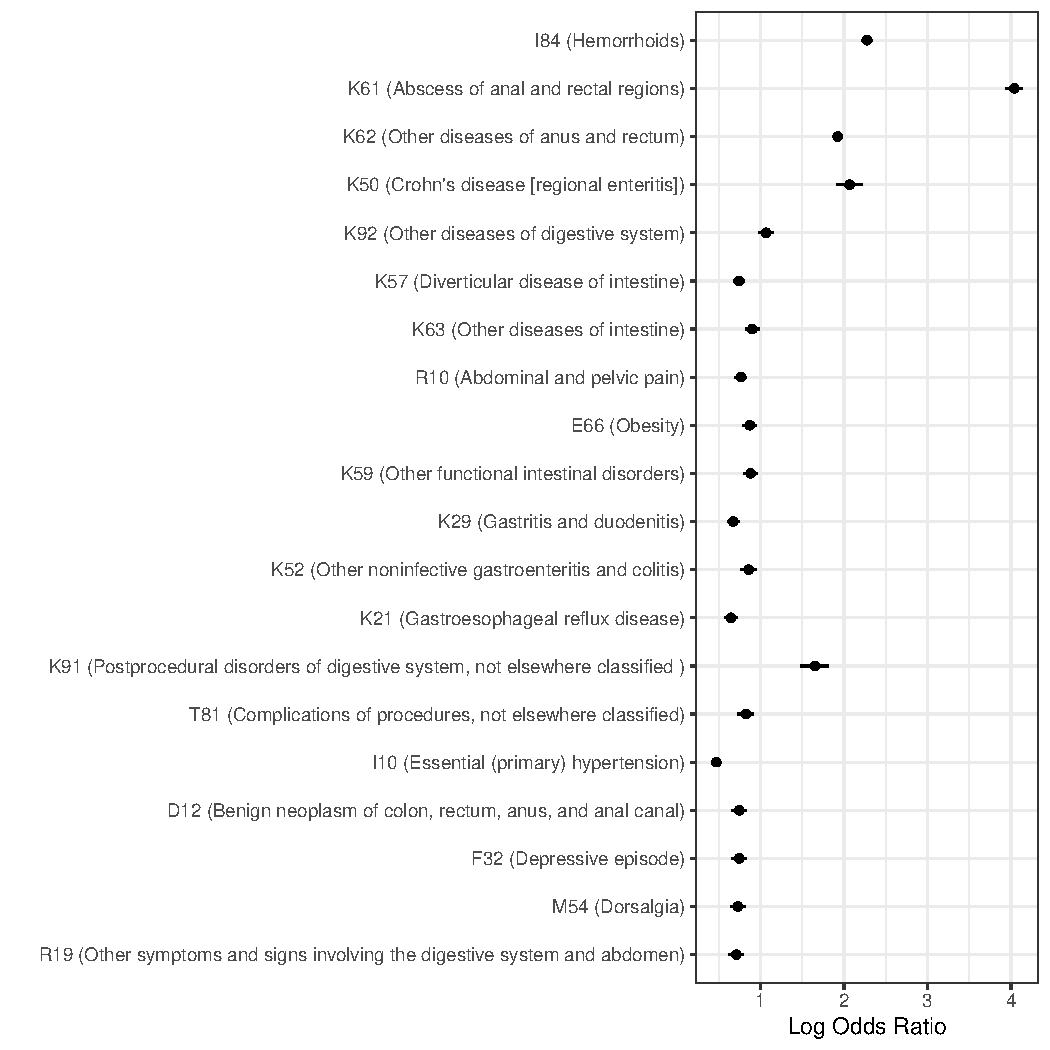
\includegraphics[width=1.0\textwidth]{pheno_enrich}
  \caption[Figure]{Top 20 ICD-10 codes enriched in pAD cases versus pAD controls ordered by Fisher's exact test P-value. Odds ratios and their 95\% confidence intervals were calculated using Fisher's exact test based on the number of pAD cases and controls with and without each particular ICD-10. Note that the control exclusion criteria in Table \ref{table:ukbb_ctrl_excl_criteria} were not applied in this analysis.}
  \label{fig:pheno_enrich}
  \end{figure}


  \subsection{UKBB GWAS}
  With the pAD case control cohort defined above, I used REGENIE to perform a pAD GWAS with White British UKBB participants \cite{Mbatchou2021-qm}. In addition to genotype QC described in the Methods section, I  excluded individuals with missing genotypes or with discordant reported and genetically-inferred sex. After this filtering a total of 4,606 pAD cases and 332,234 pAD controls remained (see Methods for genotype data quality control and imputation). In order to account for cryptic population stratification, I used 10 European-ancestry genotypic principal components, as well as sex and genotyping array as covariates in the REGENIE model. After filtering out variants with low imputation quality (INFO < 0.4) and minor allele frequency (MAF) < 0.01, a total of 9,705,089 variants were tested. After running REGENIE, I found that the summary statistics exhibited moderate genomic inflation (median $\chi^{2}=0.48$; $\lambda_{GC}=1.06$). Although $\lambda_{GC}$ values up to 1.05 are considered acceptable, higher values can be expected in GWAS with large sample sizes \cite{Price2010-zb}. In the next two sections, I will describe how I identified genome-wide significant loci, and the further quality checks I performed to ensure their validity. 
  
  \subsection{Identifying genome-wide significant loci}
  Defining genome-wide significant loci in GWAS studies is often complicated by the widespread correlation between neighbouring genome-wide significant genetic variants (i.e. linkage disequillibrium or LD). To identify pAD-associated loci, I used an LD clumping procedure, which outputs a set of \textit{index variants}, each representing a set of highly correlated variants in a locus. Additionally, LD clumping identifies nominally-associated variants that are highly correlated with the index variant at each locus (which I will refer to as LD friends; $R^{2}$ > 0.5 and P-value < 0.01; Methods). In total, seven independent loci achieved genome-wide significant association (P-value < $5\times10^{-8}$). All index variants were well-imputed (INFO $\geq$ 0.99). I also compared the index variants MAFs to population MAFs to ensure that they did not significantly deviate from expected MAFs in non-Finnish Europeans (NFE). All index variants' MAFs matched MAFs obtained from 1000 Genomes Project (1000GP), a whole-genome-sequencing-based reference cohort of diverse populations (see Methods for how MAF deviation from the general population was assessed). 

  \begin{table}[htb]
    \centering\begingroup\fontsize{10}{14}\selectfont
    \caption{Genome-wide significant index variants in the UKBB analysis. Odds ratio and their 95\% confidence intervals are shown. Minor allele frequencies (MAF) in UKBB and 1000GP (NFE) are shown in the last two columns.}
    \label{table:gws}
    \begin{tabular}[t]{|l|l|l|l|l|l|l|}
      \hline
      Chromosome & Position & Effect Allele & Odds Ratio & P-value & MAF (UKBB) & MAF (1000GP)\\
      \hline
      3 & 52,992,368 & T & 1.13 (1.08 - 1.17) & 1.5e-08 & 0.42 & 0.44\\
      \hline
      6 & 31,044,486 & G & 1.13 (1.08 - 1.18) & 2.2e-08 & 0.37 & 0.37\\
      \hline
      6 & 31,113,288 & C & 1.13 (1.08 - 1.18) & 1.1e-08 & 0.41 & 0.44\\
      \hline
      6 & 31,113,923 & A & 1.12 (1.08 - 1.17) & 3.2e-08 & 0.49 & 0.49\\
      \hline
      6 & 31,148,469 & A & 1.12 (1.08 - 1.17) & 2.6e-08 & 0.44 & 0.45\\
      \hline
      9 & 22,119,196 & T & 0.89 (0.85 - 0.93) & 2.7e-08 & 0.48 & 0.47\\
      \hline
      11 & 10,356,352 & C & 0.88 (0.84 - 0.92) & 7.3e-09 & 0.29 & 0.30\\
      \hline
      \end{tabular}

    \endgroup{}

    \end{table}

    Four of the seven loci were located in the major histocompatibility complex region (MHC; 6p21.33), and one locus in each of 3p21.1, 9p21.3 and 11p15.4. The MHC region is known to be highly polymorphic and exhibits complex and long-range LD patterns, which complicate the definition of independent loci. 
    For example, two of the four MHC loci overlapped, with their two independent index variant located less than 700 bp apart. One of the two index variants (6:31113288\_T\_C) tagged a large number of variants ($R^{2}$ > 0.8) in the locus, while the other tagged no variants (6:31113923\_A\_G). Compared to the four MHC loci, the three non-MHC loci had less complex LD patterns. All three non-MHC index variants tagged a large number of variants and there was no overlapping independent loci. Given this complexity, I performed a number of post-GWAS checks to better understand the LD structure of all seven loci, which I will describe in the next section.


    \begin{figure}[H] 
      \centering    
      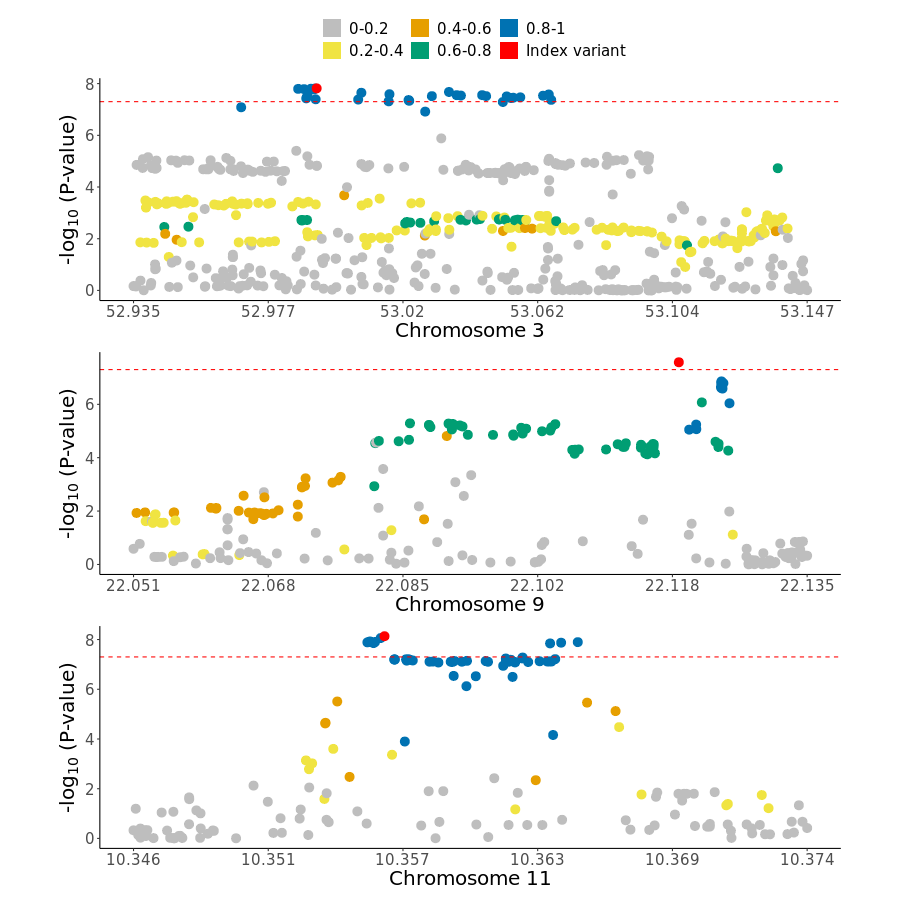
\includegraphics[width=1.0\textwidth]{Vector/ukbb_nonmhc_regional_assoc_plots.png}
      \caption[Figure]{Regional association plots for the three non-MHC loci, with position plotted on the x-axis and $-log_{10}$ P-values shown on the y-axis for each variant. Colors indicate the LD value of each variant with the index variant, and the red horizontal line indicates genome-wide significance (P-value < $5\times10^{-8}$).}
      \label{fig:ukbb_nonmhc_regional_assoc_plots}
      \end{figure}

      \begin{figure}[H] 
        \centering    
        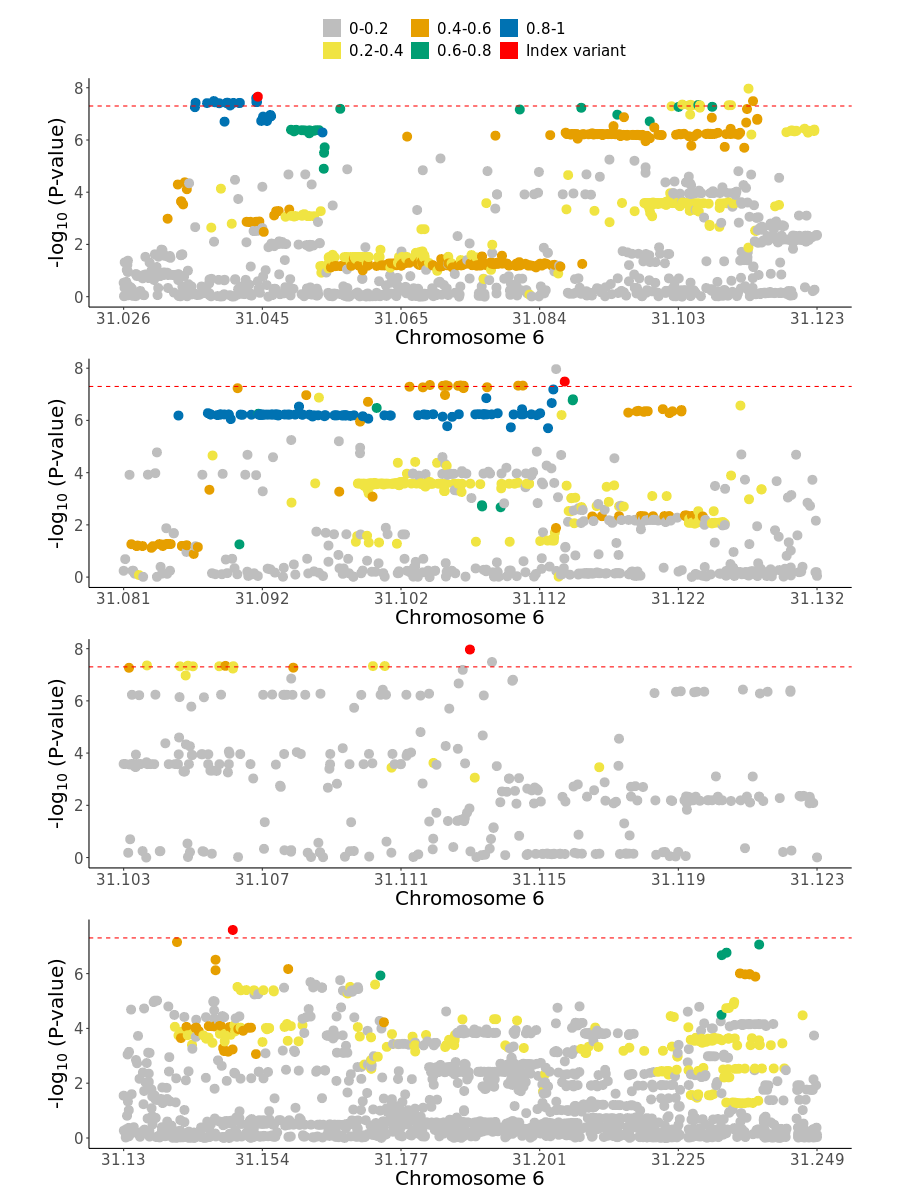
\includegraphics[width=1.0\textwidth]{Vector/ukbb_mhc_regional_assoc_plots.png}
        \caption[Figure]{Regional association plots for the four MHC loci, with position plotted on the x-axis and $-log_{10}$ P-values shown on the y-axis for each variant. Colors indicate the LD value of each variant with the index variant, and the red horizontal line indicates genome-wide significance (P-value < $5\times10^{-8}$). The second and third plots show the two overlapping MHC loci (index variants: 6:31113288\_T\_C and 6:31113923\_A\_G, respectively).}
        \label{fig:ukbb_mhc_regional_assoc_plots}
        \end{figure}

    \subsection{Post-GWAS quality checks}
    Spurious associations can seriously affect the validity of any significant results in GWAS studies. At the level of a single locus,  spurious associations can be diagnosed by assessing the relationship between variants' association strength and thir LD with the index variant. The underlying assumption is that, for a given variant in a locus, the lower its LD with the index variant, the weaker its association is expected to be. Loci where the association strength of LD friends does not "decay" as expected given their LD with the index variant are therefore paricularly problematic. Specifically, this mismatch suggests that the true underlying LD, which drives the observed association strength of LD friends, does not match the general population LD. A possible source of this mismatch may be crpytic subpopulation stratification, which often contributes to false positive associations in GWAS \cite{Hellwege2017-xf}. \\ 
    
    I investigated the seven genome-wide significant loci to ensure the association signal follows the expected LD pattern in the general population. For this check to be valid, LD needs to be computed from a suitable matching population in a diverse reference panel such as 1000GP. Additionally, each index variant needs to have a number variants LD friends. To this end, I computed LD values with the index variant at each locus from NFE in 1000GP. For each pAD-associated locus, I quantified the correlation between $R^{2}$ and P-values (on the $-log_{10}$ scale) of each index variant's LD friends. Additionally, I performed two follow-up assessments for the loci where this correlation is weak (Pearson correlation coefficient between $R^{2}$ and $log_{10}$(P-value) $\rho$ < 0.2) or cannot be computed due to a lack of LD friends. \\

    % \subsection{Index variants quality check}
    
    % All index variants were called in 1000GP except the index variant in 3p21.1 (3:52928665\_C\_T). Despite its high imputation quality in UKBB (INFO=0.93),  3:52928665\_C\_T was flagged as a low-quality site in gnomAD. Gnomad reports that 3:52928665 is a multi-allelic site located in a low-complexity region, and it is covered in fewer than 50\% of gnomAD's individuals. For this locus, I therefore computed LD with respect to the second most significant variant, which was also genome-wide significant (3:52992368\_C\_T; P-value=$1.5\times10^{-8}$). For the remaining three loci, I computed LD with the index variant for all variants in 1mbp window around the index variant. 
    
    \subsection{Relationship between P-value and LD} \label{sec:ukbb_postgwas}
  Index variants in 3p21.1, 9p21.3 and 11p15.4 had a a large number of LD friends (N=63, 66, and 49, respectively), and the P-values for each index variants' LD friends were highly correlated with $R^{2}$ ($\rho$ = 0.98, 0.74, 0.83, respectively), indicating that the P-values closely match the expected LD pattern in
  NFE. Two of the MHC loci also showed a similar pattern (index variants 6:31044486\_G\_C and 6:31148469\_G\_A in Figure \ref{fig:ukbb_ld_decay_mhc}), with a strong correlation between P-values and $R^{2}$ (Figure \ref{fig:ukbb_ld_decay_mhc}). However, this correlation did not hold for the two other overlapping MHC loci mentioned earlier, which motivated me to further investigate these two loci.
  
  \subsubsection{A complex LD pattern at two MHC loci}
  \begin{figure}[H] 
    \centering    
    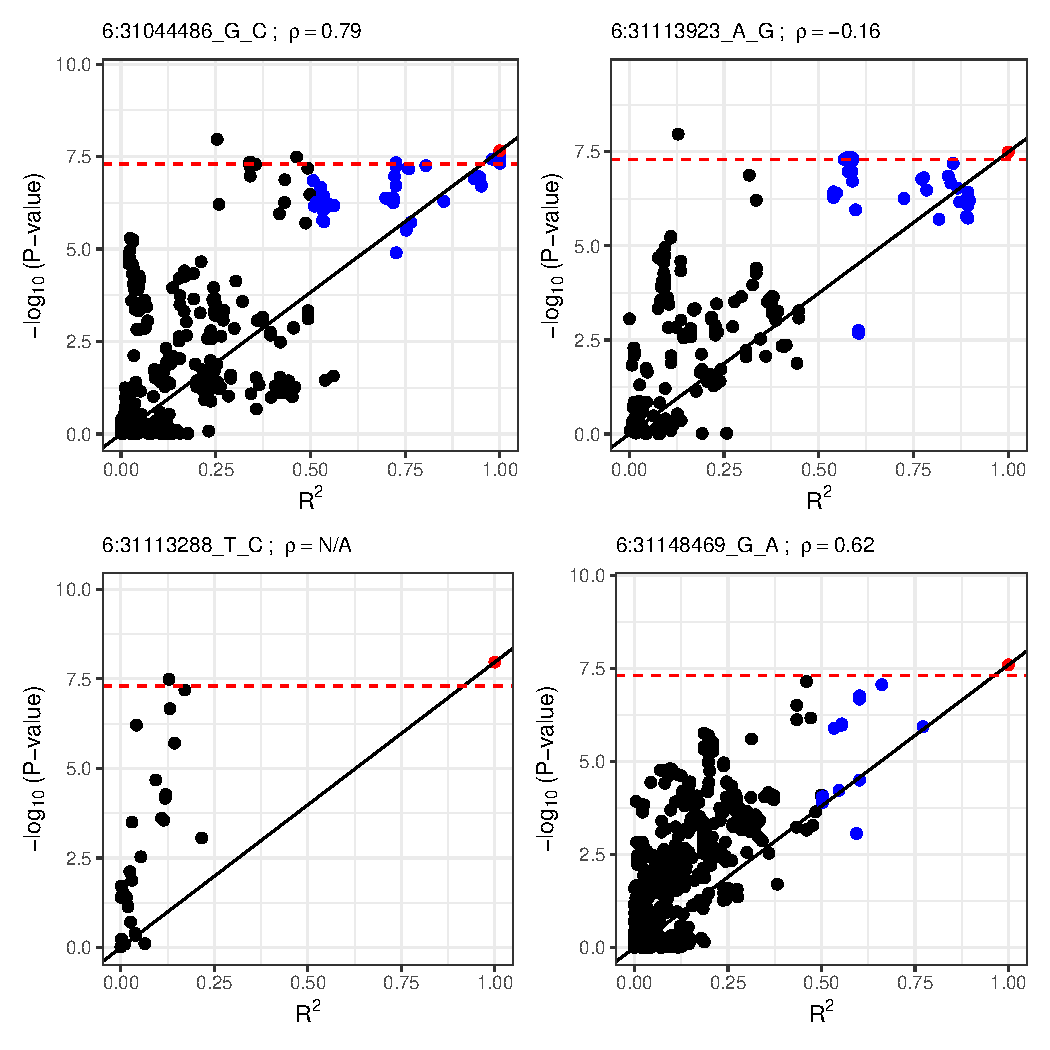
\includegraphics[width=0.8\textwidth]{ukbb_ld_decay_mhc}
    \caption[Figure]{LD decay plots showing association P-values for the four genome-wide significant loci in the MHC locus (x-axis) and each variant's $R^{2}$ with the index variant, derived from NFE in 1000GP (y-axis). Red dots and titles indicate the index variant in each locus. Blue dots indicate each index variant's LD friends, and the red horizontal line indicates genome-wide significance level (P-value < $5\times10^{-8}$). The black line is fitted to the origin (0,0), and to the point (1,$-log_{10}(P_{index\_variant})$), and shows the expected association strength given the LD with the index variant.}
    \label{fig:ukbb_ld_decay_mhc}
    \end{figure}
  First, one of MHC index variants at the two overlapping MHC loci did not tag any LD friends and therefore the correlation between P-value and $R^{2}$ could not be assessed (6:31113288\_T\_C in Figure \ref{fig:ukbb_ld_decay_mhc}). It is unclear whether the absence of LD friends for 6:31113288\_T\_C suggests that it is a truly indepent variant, or whether it is driven by a mismatch between the LD patterns in UKBB and 1000GP. Such a mismatch may lead to an underestimateion of LD between the index variant and its LD friends. To answer this question, I recalculated the LD values in 1000GP using only British individuals (GBR; N=90), and found that the index variant also did not tag any LD friends in 1000GP GBR as well. Given that 6:31113288\_T\_C is well-imputed (INFO=0.99) and common and that it is not well-tagged in both the NFE and GBR subpopulations in 1000GP, it is unlikely that the its association is driven by British-ancestry-specific LD. However, it is important to note that this does not rule out possible subpopulation stratification at this locus, which could potentially drive this association. 

  \begin{figure}[H] 
    \centering    
    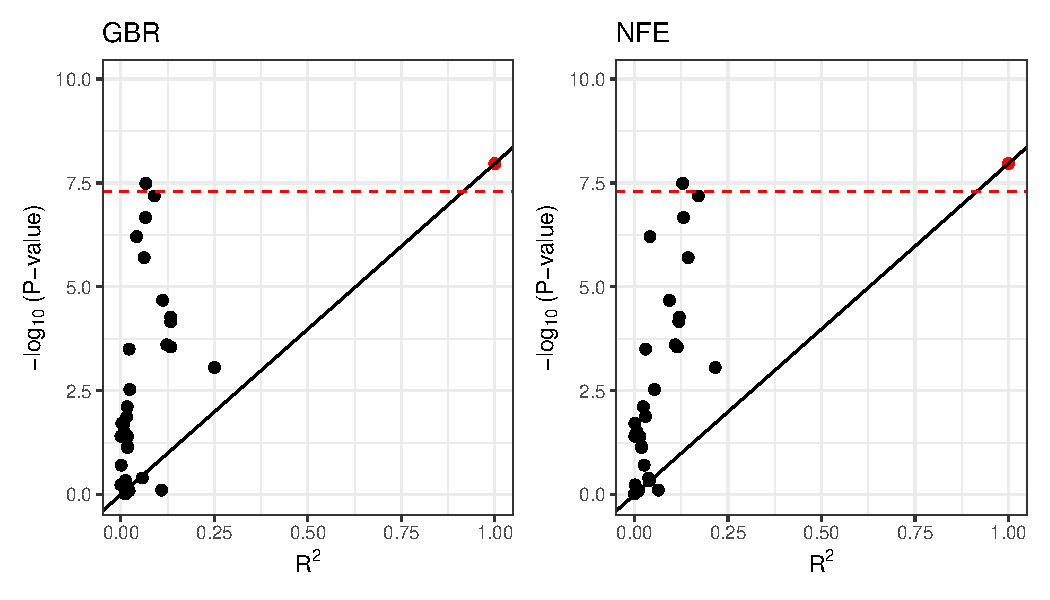
\includegraphics[width=0.8\textwidth]{ukbb_ld_decay_nfe_vs_gbr}
    \caption[Figure]{LD decay plots showing association P-values for the locus around index variant 6:31113288\_T\_C. Each variant's $R^{2}$ with the index variant, derived from NFE and GBR in 1000GP is shown on the x-axis and $-log_{10}$ P-values on the y-axis, showing that the index variant does not tag any LD friends in both NFE and GBR. Red dots indicate the index variant adn the red horizontal line indicates genome-wide significance level (P-value < $5\times10^{-8}$). The black line is fitted to the origin (0,0), and to the point (1,$-log_{10}(P_{index\_variant})$), and shows the expected association strength given the LD with the index variant.}
    \label{fig:ukbb_ld_decay_nfe_vs_gbr}
    \end{figure}

  Second, for the second overlapping locus, $R^{2}$ and P-values showed an opposite correlation (index variant 6:31113923\_A\_G in Figure \ref{fig:ukbb_ld_decay_mhc}; $\rho$=-0.16).  This inverse correlation between $R^{2}$ and P-values suggest that not all the LD friends' P-values conform to their expected P-values given their LD with the index variant. I hypothesised that the reversal of correlation may be caused by the subset of LD friends with $R^{2}$ close to the value used for defining LD friends. This subset could lead to an inverse correlation due to a stronger-than-expected P-value given their LD with the index variant. To this effect, I found that 10 LD friends had a genome-wide significant P-value (< $5\times10^{-8}$) despite all having an $R^{2}$ of 0.58 with the index variant. When I repeated the LD clumping procedure at this locus with a higher clumping $R^{2}$ cutoff (=0.6), I found that this subset of variants constituted a new genome-wide significant locus. This suggests that the identification of independent loci at this region is senstitive to the choice of LD clumping $R^{2}$ cutoff, which further complicates the identification of independent loci at this region. 
  

  



      \subsection{Finngen GWAS}
      Similar to UKBB, other national biobanks with genetic, clinical and phenotypic data are available. Although most national biobanks limit access to their individual-level genotype and phenotype data to approved researchers only, results from secondary analyses, including GWAS summary statistics, are made publicly available. \\

      FinnGen is a national biobank whose aim is to collect genetic and phenotypic data for 500,000 Finnish individuals. The latest data freeze (Data Freeze 9) has genotyped over 377,000 individuals and has carried out GWAS for over 2,200 clinical endpoints. FinnGen uses a different clinical coding system from ICD to organise phenotypes into endpoints (FinnGen endpoints). There are two main differences between UKBB and FinnGen in terms of their clinical code structure. First, most FinnGen endpoints have parallel ICD codes, but additional FinnGen endpoints are created at request. Bespoke endpoints define certain inclusion or exclusion criteria based on ICD codes, or sometimes combine codes from different ICD chapters to create a new endpoint. Second, FinnGen endpoints are curated by experts in each field and are constantly reviewed in different FinnGen data freezes. They are brodaly classified as \textit{core endpoints}, or \textit{non-core endpoints}. Basic statistics such as prevalence and gender ratios are calculated for all FinnGen endpoints, while GWAS is conducted only for core endpoints.\\

ICD-10 code K60 corresponds to FinnGen endpoint K11\_FISSANAL (Fissure and fistula of anal and rectal regions). K11\_FISSANAL defines cases and controls similar to my UKBB cohort definition outlined in Table \ref{table:ukbb_ctrl_excl_criteria}. However, K11\_FISSANAL was considered a core endpoint only until Data freeze 7, and GWAS summary statistics for K11\_FISSANAL are threfore unavailable in later data freezes. 

\subsection{Identification of genome-wide significant loci in Finngen}

In order to investigate if the seven UKBB genome-wide significant loci replicated in an independent cohort and to identify additional loci, I downloaded GWAS summary statistics for FinnGen's clinical endpoint K11\_FISSANAL. As of data freeze 7, Finngen reports 6,610 pAD cases and 253,186 controls. There was no further information regarding the subtypes of pAD (e.g. numbers of fissure and fistula cases), and it is therefore unclear if the composition of FinnGen's pAD case cohort is similar to the UKBB pAD case cohort. Understanding the differences in subphenotype composition of each cohort is important to understand if differences in association at genome-wide significant loci is driven by genetic factors (e.g. differences in MAFs or LD structure) or by phenotypic differences between the cohorts. 

After I filtered out variants with MAF < 0.01, a total of 9,054,355 variants remained. There was an acceptable level of genomic inflation (median $\chi^{2}$=0.495; $\lambda_{GC}$=1.089). To identify genome-wide significant loci, I used an LD clumping approach similar to the UKBB analysis, with the only difference being that I calculated LD from Finnish Europeans in 1000GP (FE; N=99). I found three genome-wide significant non-MHC loci: 1p34.2, 6p25.3 and 12q24.21 (P-value < $5\times10^{-8}$). Imputation quality information was not available in the downloaded summary statistics, so I was not able to confirm if the index variants had good imputation quality. However, the index variants' MAFs matched MAFs derived from FE in 1000GP, suggesting that they are imputed or genotyped with high confidence (Table \ref{table:gws_finngen}). Furthermore, I performed similar post-GWAS checks to UKBB to ensure the P-value of the index variants LD friends match their expected values given their LD with the index variant. All three showed a good decay of P-values with LD ($\rho$=0.92, 0.74 and 0.44, respectively; Figure \ref{fig:finngen_regional_assoc_ld_decay_plots})

\begin{table}[htb]
  \centering\begingroup\fontsize{10}{12}\selectfont
  \caption{Genome-wide significant index variants in the FinnGen GWAS. Odds ratio and their 95\% confidence intervals are shown. Minor allele frequencies (MAF) in UKBB and 1000GP (FE) are shown in the last two columns.}
  \label{table:gws_finngen}
  \begin{tabular}[t]{|l|l|l|l|l|l|l|}
  \hline
  Chromosome & Position & Effect Allele & Odds Ratio & P-value & MAF (Finngen) & MAF (1000GP)\\
  \hline
  1 & 39,817,036 & T & 1.14 (1.09 - 1.19) & 7.2e-10 & 0.21 & 0.22\\
  \hline
  6 & 1,771,278 & T & 0.9 (0.87 - 0.93) & 6.7e-09 & 0.42 & 0.39\\
  \hline
  12 & 114,235,969 & T & 1.11 (1.07 - 1.15) & 7.0e-09 & 0.47 & 0.47\\
  \hline
  \end{tabular}
  \endgroup{}
  \end{table}

\begin{figure}[H] 
  \centering    
  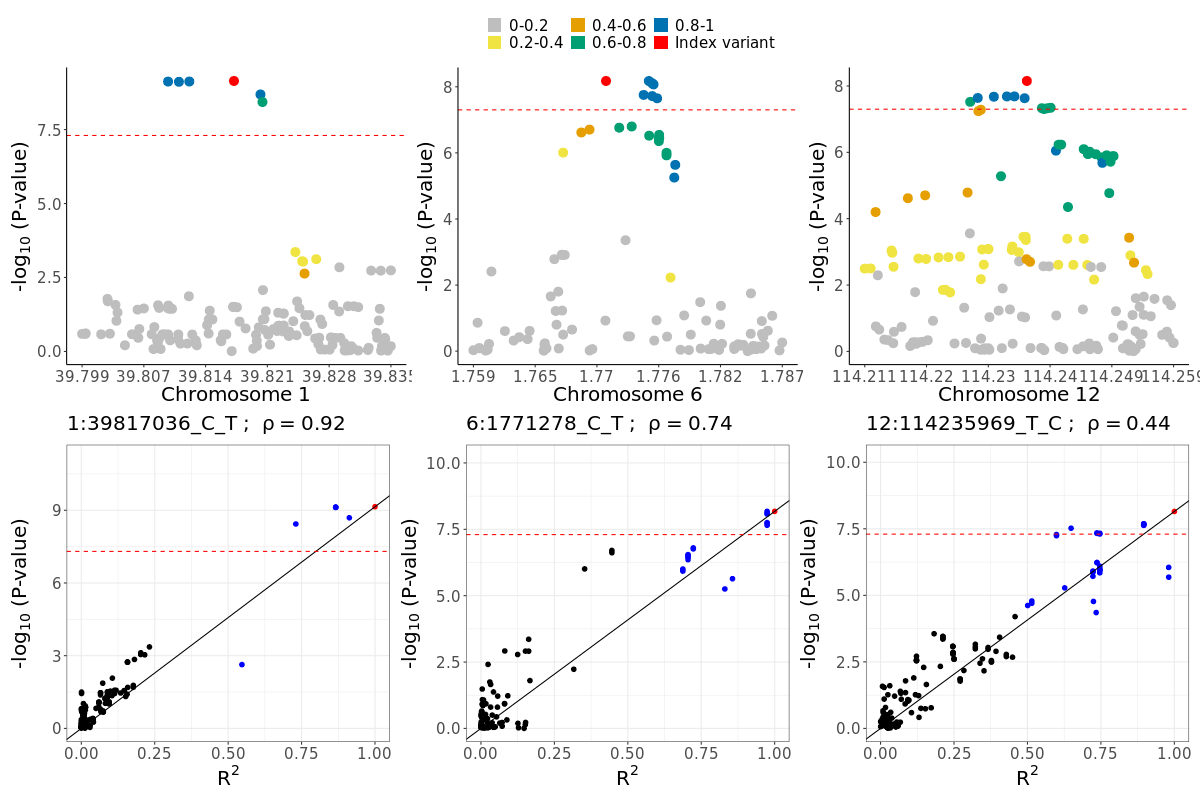
\includegraphics[width=1.0\textwidth]{Vector/finngen_regional_assoc_ld_decay_plots.png}
  \caption[Figure]{(Top) Regional association plots for the three FinnGen loci, with position plotted on the x-axis and $-log_{10}$ P-values shown on the y-axis for each variant. Colors indicate the LD value of each variant with the index variant, and the red horizontal line indicates genome-wide significance (P-value < $5\times10^{-8}$). (Bottom) LD decay plots showing association P-values for the three genome-wide significant loci in FinnGen (x-axis) and each variant's $R^{2}$ with the index variant, derived from FE in 1000GP (y-axis). Red dots and titles indicate the index variant in each locus. Blue dots indicate each index variant's LD friends. The red horizontal line indicates genome-wide significance level, and the black line is fitted to the origin (0,0), and to the point (1,$-log_{10}(P_{index\_variant})$), and shows the expected association strength given the LD with the index variant.}
  \label{fig:finngen_regional_assoc_ld_decay_plots}
  \end{figure}




\subsection{Replication of UKBB loci in Finngen}

\subsubsection{LD pattern in Finnish Europeans}
In GWAS studies, the true causal variant in an associated locus is often unknown due to LD between variants. Moreover, it is often the case that the true causal variant may not even be genotyped in array-based GWAS studies, or may not be imputed due to different imputation protocols and QC metrics being used in different GWAS. When assessing replication of a GWAS locus between two cohorts, it is therefore important to ensure that their LD structure is similar. Indeed, a lack of GWAS hit replication is sometimes driven by a difference in LD patterns between the two studies under comparison, one of which may not have genotyped or imputed any variants that tag the true causal variant in its respective population \cite{Kraft2009-xg}. Finnish Europeans (FE) and NFE are known to exhibit systematic difference in their LD strucure, which may affect the ability to replicate the pAD-associated loci discovered in the UKBB. To compare the LD pattern between FE and NFE at the pAD-associated loci, I computed the LD between each variant and the index variant in the FE and NFE subpopulations of 1000GP.\\





% \begin{figure}[H] 
%   \centering    
%   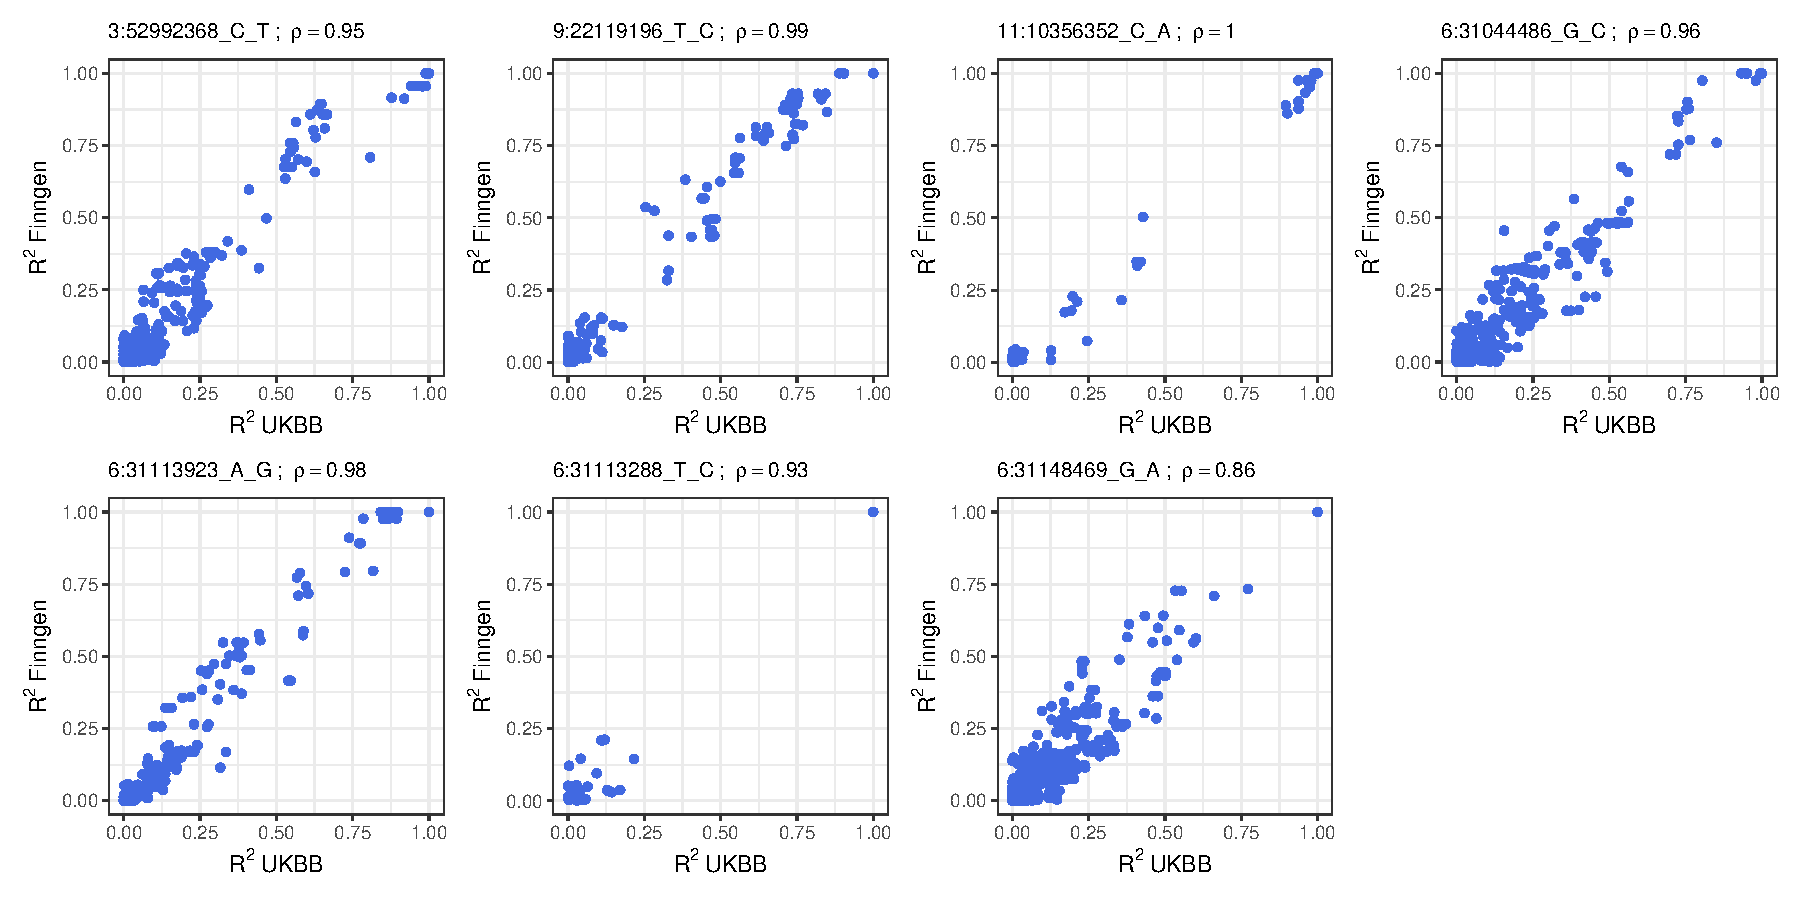
\includegraphics[width=1.0\textwidth]{ukbb_finngen_ld_plot}
%   \caption[Figure]{$R^{2}$ between variants and the index variant in the four pAD-associated loci in non-Finnish Europeans (x-axis) and Finnish Europeans (y-axis). $R^{2}$ values are derived from the 1000GP. Pearson correlation coefficients and index variants are indicated on top of each figure.}
%   \label{fig:ukbb_finngen_ld_plot}
%   \end{figure}

\begin{figure}[H]
  \centering
  \begin{subfigure}[b]{1.0\textwidth}
      \centering
      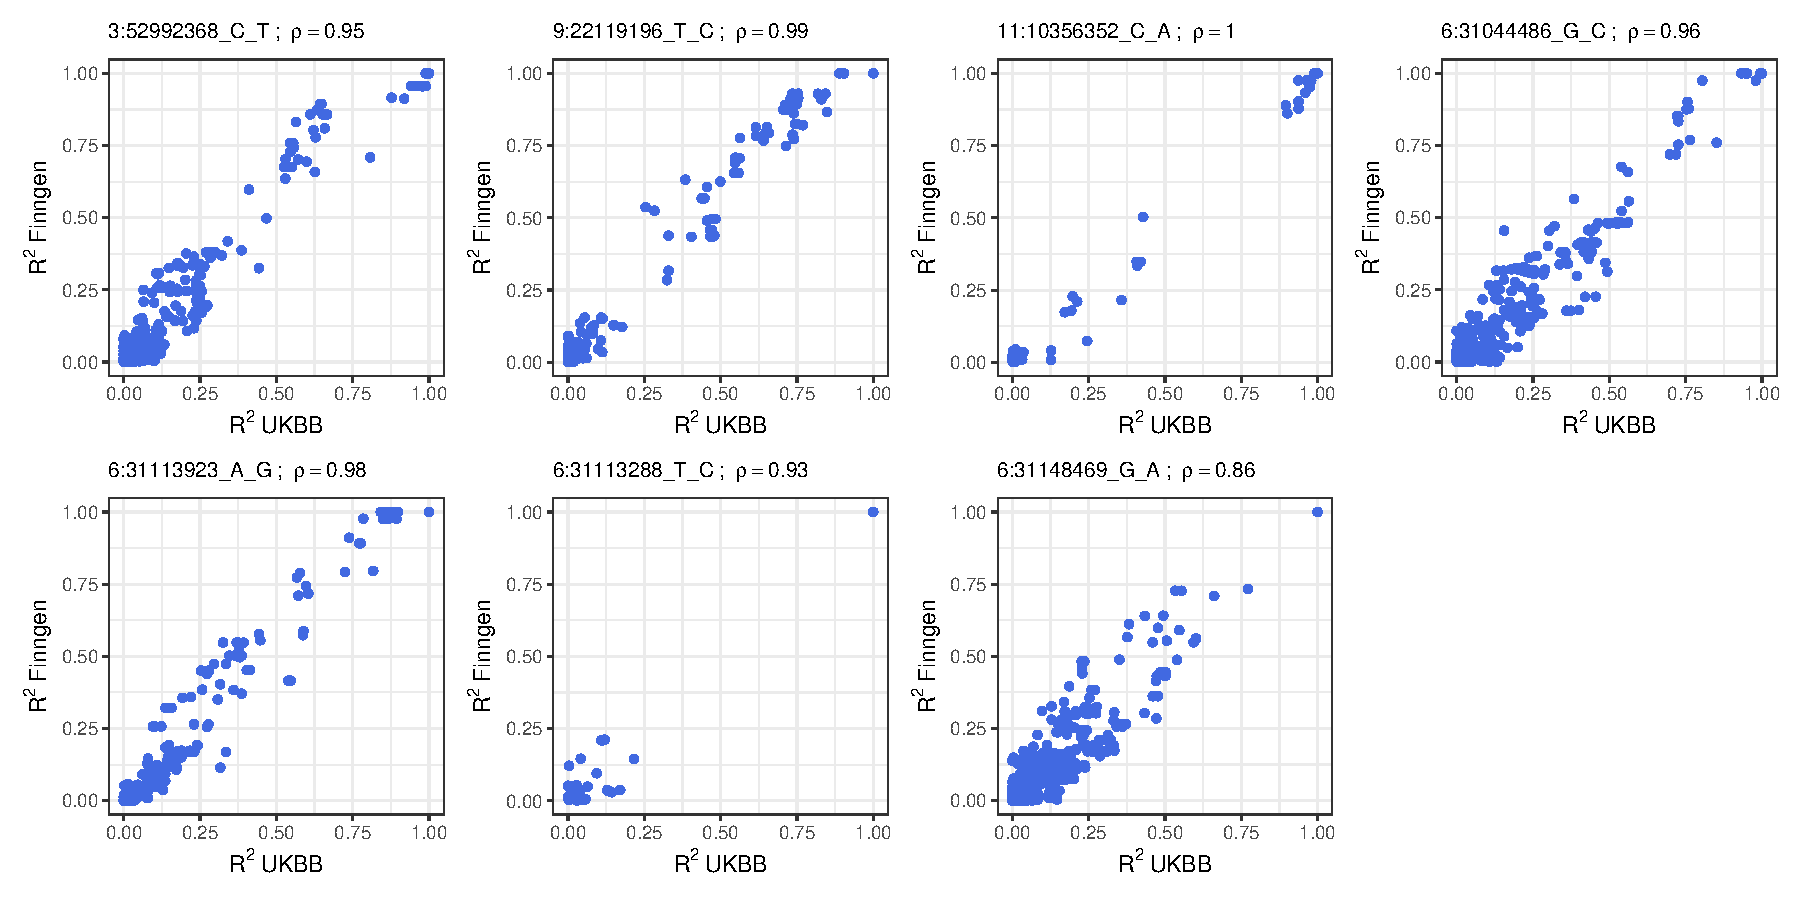
\includegraphics[width=\textwidth]{ukbb_finngen_ld_plot}
      \caption{}
      \label{fig:ukbb_finngen_ld_plot}
  \end{subfigure}
  \hfill
  \begin{subfigure}[b]{1.0\textwidth}
      \centering
      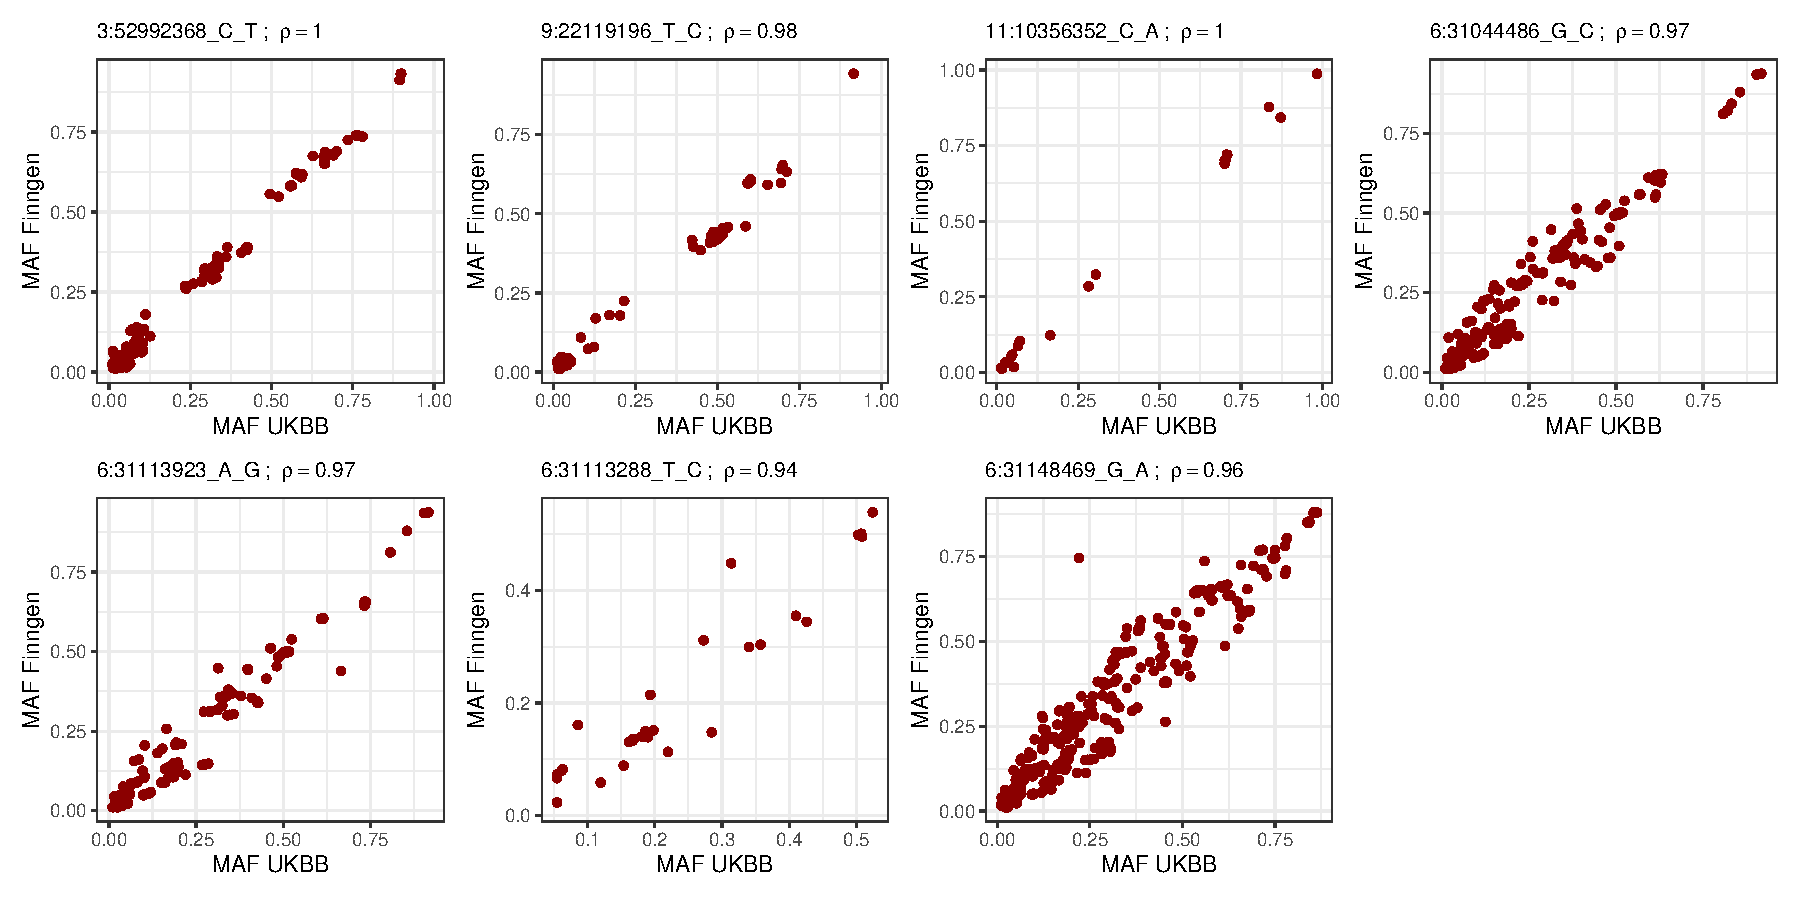
\includegraphics[width=\textwidth]{ukbb_finngen_maf_plot}
      \caption{}
      \label{fig:ukbb_finngen_maf_plot}
  \end{subfigure}


     \caption{(a) $R^{2}$ between variants and the index variant in the seven UKBB loci in non-Finnish Europeans (x-axis) and Finnish Europeans (y-axis). $R^{2}$ values are derived from the 1000GP. Pearson correlation coefficients and index variants are indicated on top of each figure. (b) MAF of all variants in the UKBB (x-axis) and FinnGen (y-axis).}
     \label{fig:ld_maf_replication_ukbb_in_finngen}
\end{figure}
I found that MAF was nearly perfectly correlated in NFE and FE in all seven pAD-associated loci ($\rho$ > 0.94; Figure \ref{fig:ld_maf_replication_ukbb_in_finngen}a). $R^{2}$ were also strongly correlated in all loci ($\rho$ > 0.86; Figure \ref{fig:ld_maf_replication_ukbb_in_finngen}b). Notably, despite a strong $R^{2}$ correlation, 6:31113288\_T\_C did not have any LD friends in FE, similar to GBR and NFE, and the strong correlation at this locus was driven by variants with a low $R^{2}$ with the index variant. Overall, witht the exception of 6:31113288\_T\_C which did not have any LD friends in FE, both MAF and the LD structure were consistent across all pAD-associated loci between NFE and FE. Replication of UKBB hits can therefore be reasonably assessed in the FinnGen GWAS.\\

\subsubsection{UKBB non-MHC loci replicate in Finngen}
To test the replication of the UKBB hits, I adopted an approach that takes into account subtle differences in LD between FE and NFE. UKBB index variants may not necessarily tag the true causal variants in FE, and an absence of replication of the exact UKBB index variants in FinnGen does not therefore indicate the lack of association at pAD-associated loci. Therefore, I performed the replication using each index variant and their LD friends in FinnGen ($R^{2}$ > 0.5 in FE). I found that all non-MHC loci replicated (Bonferroni-corrected P-value < $7\times10^{-3}$). Additionally, all top variants in FinnGen were in high LD with the UKBB index variants ($R^{2}$ > 0.86). Conversely, none of the MHC loci replicated in FinnGen (Table \ref{table:replication_ukbb_in_finngen}). Possible explanations of why these loci fail replication are outlined in the Discussion section. \\



\begin{table}[H]
  \caption{Replication of UKBB genome-wide significant loci in FinnGen. The first and third columns show the UKBB index variant and its UKBB P-value, respectively. The second and fourth columns show FinnGen's top variant at each locus, and its FinnGen P-value, respectively. The last column shows the LD between FinnGen's top variant and the index variant in 1000GP FE.}
  \label{table:replication_ukbb_in_finngen}
  \centering
  \begin{tabular}[t]{llllr}
  \toprule
  UKBB & Finngen & P-value UKBB & P-value Finngen & $R^{2}$\\
  \midrule
  3:52992368\_C\_T & 3:53056474\_C\_T & 1.5e-08 & 3.4e-04 & 0.96\\
  6:31044486\_G\_C & 6:31044486\_G\_C & 2.2e-08 & 5.7e-02 & 1.00\\
  6:31113923\_A\_G & 6:31113923\_A\_G & 3.2e-08 & 3.9e-02 & 1.00\\
  6:31113288\_T\_C & 6:31113288\_T\_C & 1.1e-08 & 1.5e-01 & 1.00\\
  6:31148469\_G\_A & 6:31148469\_G\_A & 2.6e-08 & 9.9e-01 & 1.00\\
  \addlinespace
  9:22119196\_T\_C & 9:22090936\_C\_T & 2.7e-08 & 1.5e-03 & 0.86\\
  11:10356352\_C\_A & 11:10363421\_G\_A & 7.3e-09 & 1.7e-07 & 0.98\\
  \bottomrule
  \end{tabular}
  \end{table}
  \subsection{Replication of FinnGen loci in UKBB}
  Following the same replication approach, I tested the replication of FinnGen's three genome-wide significant loci in the UKBB. For each of the three index variants, I identified all their LD friends in the UKBB, using $R^{2}$ values derived from 1000GP NFE. Then, I tested if any of the LD friends show evidence of replication and  found evidence of replication for all three loci in the UKBB (Bonferroni-corrected P-value < 0.017).

  \begin{table}[H]
    \caption{Replication of FinnGen's genome-wide significant loci in the UKBB. The first and third columns show the FinnGen index variants and their FinnGen P-value, respectively. The second and fourth columns show UKBB's top variants at the locus, and their FinnGen P-value, respectively. The last column shows the LD between the UKBB top variant and the index variant in 1000GP NFE.}
    \label{table:replication_finngen_in_ukbb}
    \centering
    \begin{tabular}[t]{llllr}
    \toprule
    Finngen & UKBB & P-value Finngen & P-value UKBB & $R^{2}$\\
    \midrule
    1:39817036\_C\_T & 1:39809417\_A\_T & 7.2e-10 & 2.3e-07 & 0.74\\
    6:1771278\_C\_T & 6:1775480\_A\_T & 6.7e-09 & 4.7e-05 & 0.91\\
    12:114235969\_T\_C & 12:114247766\_A\_G & 7.0e-09 & 4.5e-04 & 0.74\\
    \bottomrule
    \end{tabular}
    \end{table}


    \subsection{Meta-analysis of UKBB and FinnGen}
    Meta-analyisis between GWAS cohorts is commonly used to increase statistical power to identify genome-wide significant loci. Practically, meta-analysis is carried out when the are constraints on sharing individual-level data, or when genotype data from several studies cannot be combined \cite{Evangelou2013-rn}. In these cases, meta-analysis of association summary statistics is the preferred analytical approach, and there is ample evidence that it achieves similar statistical power as combining genotype data from several studies \cite{metal_docs}. \\

    Several factors affect the effectiveness of genome-wide meta-analyses, including genetic factors as well as factors related to the pAD case cohort. First, over the last several thousand years, Finnish Europenas were admixed with several Central Asian and East Asian populations, as well as Non-Finnish Europeans \cite{Qin2015-jb}. This admixture led to systematic differences between Finnish and Non-Finnish Europeans, both in terms of allele frequencies and LD strucure.  In addition, local subpopulation stratification in both cohorts may drive spurious associations, which might be amplified in a meta-analysis if not properly accounted for. Second, although case and control inclusion criteria are similar between the two cohorts, it is not obvious if the composition of the pAD case cohort is also similar. Similar to the ICD-10 code used in the UKBB analysis to identify anal fissures and fistula cases, the corresponding FinnGen's clinical endpoint covers several clinical diagnosis. I have shown in Table \ref{table:ukbb_level2_nums} that the proportion of anal fissures and fistula cases is roughly 3:2. Since FinnGen's individual-level data are not publicly available, I could not confirm if the proportion of anal fissure and fistula cases are similar. Moreover, it is unclear if FinnGen's case cohort is enriched in any other clinical endpoints compared to FinnGen's control cohort. Showing that the pAD cases are enriched in the same disorders (e.g. haemorrhoids and anal abscess) can serve as an important phenotypic quality control check to ensure that both cohorts are as homogenous as possible, and maximises the ability of a meta-analysis to identify genetic variants associated with pAD risk.

    \subsubsection{Meta-analysis and identification of genome-wide significant loci}
    I performed a fixed-effects meta-analysis between UKBB and FinnGen summary statistics using effect size estimates and standard errors using METAL (see Methods for more details). After filtering out variants with MAF < 0.01 and with low imputation score (INFO < 0.4), the two GWAS summary statistics had an intersection of 7,663,827 variants and a total of 11,096,129 variants across the two cohorts. Of these, 2,041,145 variants were specific to UKBB and 1,390,527 were specific to FinnGen. Given that 31\% of variants were unique to one of the two GWAS, I did not remove them from their respective summary statistics file. It is important to note, however, that this choice may favour variants that are available in both studies. Additionally, I enabled METAL's \Verb+GENOMICCONTROL ON+ option to correct genomic inflation in each of the two summary statistics before performing the meta-analysis. The resulting meta-analysed summary statistics showed no evidence of genomic inflation ($\lambda_{GC}$=1.02).\\

    I used LD clumping to identify genome-wide significant loci and a representative index variant for each locus. Because I performed a meta-analysis between FE and NFE summary statistics, I performed LD clumping separately with an LD panel from each of the two populations, and found 18 genome-wide significant loci (P-value < $5\times10^{-8}$). Furthermore, I compared the association signal and LD for each locus using same two reference panels. Six of these loci either showed weak or inverse correlation between P-values and $R^{2}$ derived from either NFE and FE ($\rho$ < 0.2), and were therefore removed from the rest of the downstream analyses (more details in Methods).\\
    
    Furthermore, for these 12 loci, I tested whether the index variants' effect size estimates were consistent between UKBB and FinnGen using Cochran's Q test, which is implemented in METAL (Methods). A strong deviation from the null hypothesis that effect sizes are similar between UKBB and FinnGen reflects uncertainty around the meta-analysed effect size estimate. To this end, I found no evidence of heterogenity for any of the 12 index variants ($P_{het} < 4\times10^{-3}$).

    \begin{table}[H]
      \caption{Meta-analysis genome-wide significant loci (P-value < $5\times10^{-8}$), showing the index variant at each locus, odds ratio in the UKBB, FinnGen, and meta-analysis. The last column shows the P-value of the effect size heterogeneity test.}
      \label{table:meta_gws}
      \centering
      \begin{tabular}[t]{p{0.25\linewidth}p{0.1\linewidth}p{0.1\linewidth}p{0.1\linewidth}p{0.1\linewidth}p{0.1\linewidth}}
      \toprule
      Index variant & Meta-analysis P-value & OR (UKBB) & OR (FinnGen) & OR (Meta-analysis) & $P_{het}$\\
      \midrule
      3:53034026\_C\_T & 7.5e-10 & 1.13 & 1.07 & 1.09 & 0.05\\
      \addlinespace
      5:64868326\_TTTC\_T & 2.0e-08 & 0.89 & 0.94 & 0.92 & 0.05\\
      \addlinespace
      6:1775202\_G\_A & 1.0e-11 & 0.91 & 0.9 & 0.9 & 0.80\\
      \addlinespace
      6:31121854\_C\_T & 4.2e-08 & 1.11 & 1.06 & 1.08 & 0.08\\
      \addlinespace
      6:31253340\_T\_C & 3.8e-08 & 1.1 & 1.07 & 1.08 & 0.24\\
      \addlinespace
      6:133260944\_G\_A & 4.7e-08 & 1.11 & 1.08 & 1.1 & 0.42\\
      \addlinespace
      7:2524404\_G\_A & 4.1e-08 & 1.14 & 1.13 & 1.14 & 0.76\\
      \addlinespace
      8:70735125\_A\_G & 3.9e-11 & 0.83 & 0.82 & 0.83 & 0.94\\
      \addlinespace
      8:70993166\_AAGTT\_A & 1.2e-10 & 0.83 & 0.82 & 0.82 & 0.75\\
      \addlinespace
      9:22124505\_A\_T & 2.1e-08 & 0.9 & 0.95 & 0.92 & 0.05\\
      \addlinespace
      11:10356352\_C\_A & 1.3e-13 & 0.88 & 0.91 & 0.89 & 0.27\\
      \addlinespace
      12:114235969\_T\_C & 4.2e-10 & 1.07 & 1.11 & 1.09 & 0.20\\
      \bottomrule
      \end{tabular}
      \end{table}


  %   Why performed meta-analysis? 
  %   \begin{itemize}
      
      
  %     \item \textbf{Pros} 
  %     \item Any concerns about difference in phenotype definitions: 
  %     \item reasons why that might be the case (difference in proporion - biases introduced by different clinical systems - differences in prevalence)
  %     \item Any concerns about differences in LD and MAF and subpopulation stratification and how that was adressed
  %     \item \textbf{Cons}
  %     \item  Maximise in power
  %     \item pop strat can be taken care of by adjusting lambda gc
  %     \item Individual-level data are required for better definition of phenotype
  % \end{itemize}
    
 

  \subsection{Disentangling the genetic effect of pAD-associated variants on related intestinal disorders}

  In section \ref{section:pheno_enrich}, I analysed the composition of the pAD case cohort and showed that it is significantly enriched with 198 ICD-10 clinical codes compared to pAD controls. I hypothesised that this enrichment was also reflected at the level of genetic risk predisposition. To confirm this, I performed a genetic correlation analysis using LD score regression (LDSC). LDSC is a method that quantifies the shared genetic risk between two traits using only GWAS summary statistics, and is therefore a widely-used method to investigate the genetic relationship between a trait of interest and other related traits without the need to access individual-level data. To this end, I first downloaded GWAS summary statistics from the Pan-UKBB project, a large-scale analysis that performed a UKBB case-control GWAS analysis for 7,228 UKBB phenotypes including all ICD-10 codes. I carried out a genetic correlation analysis between the pAD meta-analysis and the Pan-UKBB haemorrhoids GWAS, and found strong evidence of high genetic correlation (ICD-10 code I84; P-value=$5.37\times10^{-26}$; $r_{g}$=0.66). To validate this correlation, I repeated the genetic correlation analysis using a larger haemorrhoids GWAS of over 900,000 individuals by Zheng et al. 2021 \cite{Zheng2021-ss}. I found a similar genetic correlation estimate that was even more significant than the estimate from the Pan-UKBB analysis ($r_{g}$=0.63; P-value=$10^{-62}$).
  

  The existence of a strong genetic correlation and enrichment of haemorrhoids could be explained by several factors. First, pAD could be a co-morbidity of haemorrhoids, in a similar way that Type 2 diabetes and obesity are comorbidities. This could be a result of the same risk factors (genetic or otherwise) underlying both diseases, potentially with varying effect sizes. Alternatively, clinical diagnostic factors could also account for this overlap. Both diseases are among the differential diagnoses for patients presenting with rectal pain, swelling, bleeding and discharge. Therefore, a patient suffering from inflammed haemorrhoids is more likely to be diagnosed if they also suffer from pAD (e.g. after performing rectal examination). \\ 

Bias introduced by clinical diagnostic factors cannot be completely addressed with observational data, as this will require constructing pAD case-control cohorts where haemorrhoids cases are  balanced in both cases and controls. However, the impact of such bias could also be assessed by performing a pAD GWAS where haemorrhoids cases are excluded from cases and controls (pADexclHaem), and a haemorrhoids GWAS where pAD cases are excluded from cases and controls (HaemexclpAD). Comparing the genetic association effect sizes of the previously reported 12 index variants between pADexclHaem and HaemexclpAD may give an indication as to which genetic variants are likely to underlie both diseases and which are likely to be specific to pAD. \\

Constructing the two cohort requires access to a individual-level phenotypic data in both UKBB and FinnGen. Therefore, I tested the hypothesis that effect sizes are different between the haemorrhoids and pAD in the UKBB only. To construct the HaemexclpAD case and control cohorts, I selected individuals who have been diagnosed with ICD-10 code I84 or ICD-9 code 455 in at least one inpatient episode as cases and excluded individuals with ICD-10 code K60 or ICD-9 code 565 from both cases and controls. Similarly, for pADexclHaem, I selected individuals who have been diagnosed with ICD-10 code K60 or ICD-9 code 565 in at least one inpatient episode and excluded individuals with ICD-10 code I84 or ICD-9 code 455 from both cases and controls. Additionally, I applied the same control exclusion criteria in Table \ref{table:ukbb_ctrl_excl_criteria}. 

\begin{figure}[H]
  \centering    
  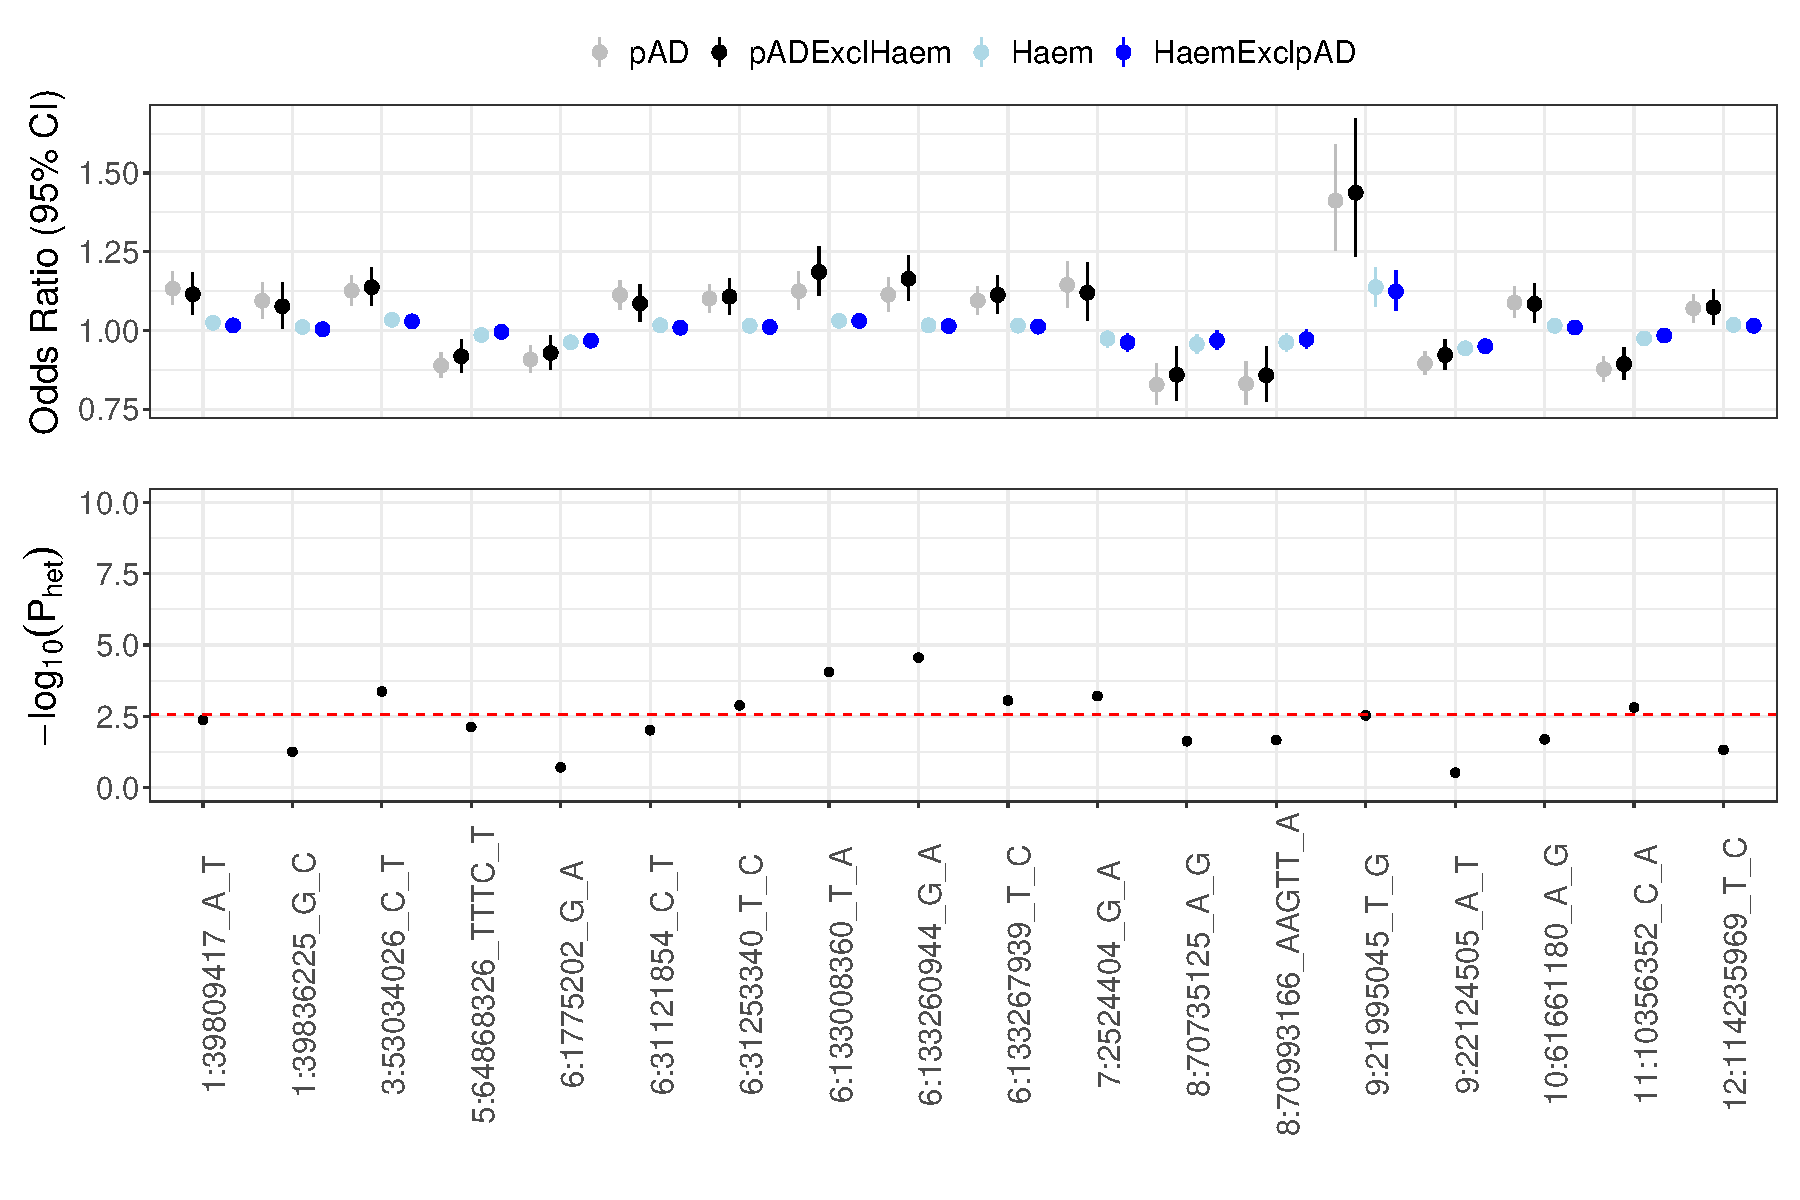
\includegraphics[width=1.0\textwidth]{combined_forest_het_plt}
  \caption[Figure]{Top plot shows the ffect sizes of the 12 pAD-assocaited index variants from four UKBB case/control cohorts: pAD in grey ($N_{case}$=4,606), pADExclHaem in black ($N_{case}$=2,799), Haem in light blue ($N_{case}$=29,285), and HaemExclpAD in blue ($N_{case}$=27,477). Bottom plot shows the heterogeneity of effect-size P-value ($P_{het}$) between the two disjoint GWAS analyses: pADExclHaem and HaemexclpAD. The red dotted line shows $P_{het}$ significance threshold ($P_{het} < 3\times10^{-3}$).}
  \label{fig:combined_forest_het_plot}
  \end{figure}

I tested the association of each of the 12 pAD-associated index variants with each of the four phenotypes described above. First, I examined if any of the index variants were associated with the two haemorrhoids phenotypes Haem and HaemExclpAD. Since I performed a targeted association test, I set a more permissive assocition threshold for declaring significance than normally used to declare genome-wide assoctions (P-value < $3\times10^{-3}$). Despite the large difference in statistical power between the two haemorrhoids cohorts and the two pAD cohorts, I found that only three of the tested index variants achieved significant association with haemorrhoids (index variants: 3:53034026\_C\_T, 6:1775202\_G\_A, and 9:22124505\_A\_T). Additionally, all three variants were significant in both Haem and HaemExclpAD, suggesting that the exclusion of pAD cases from the haemorrhoids cohort has little impact on their association. Moreover, 3:53034026\_C\_T showed significant evidence of effect size heterogeneity between pADExclHaem and HaemExclpAD ($P_{het}$ < $3\times10^{-3}$; Figure \ref{fig:combined_forest_het_plot}), with a significantly larger effect on pADExclHaem ($OR_{pADExclHaem}=1.14-1.2$ and $OR_{HaemExclpAD}=1.03-1.05$).

Although the rest of the 12 index variants did not show a significant association with the two haemorrhoids definitions, they exhibited a pattern similar to 3:53034026\_C\_T. Specifically, four of the 12 pAD-associated index variants had significantly smaller effect sizes in HaemexclpAD than in pADexclHaem ($P_{het}$ < $3\times10^{-3}$; Figure \ref{fig:combined_forest_het_plot}). Moreover, five additional variants had suggestive evidence of heterogeneity of effect ($P_{het}$ < 0.05), and in all these cases the effect size was larger in pADExclHaem than in HaemExclpAD. 

Two conclusion can be made from this analysis. First, despite a much larger sample size in favour of the haemorrhoids cohorts, only three pAD-associated index variants were also associated with haemorrhoids, even with a relatively lenient threshold for association. Second, despite their nominal association with haemorrhoids, these three variants (and indeed all other variants) had a consistently smaller effect size on HaemExclpAD than pADExclHaem, and for 3:53034026\_C\_T that difference in effect size was significant. More importantly, this pattern was observed for all 12 index variants, despite the lack of power to detect a significant heterogeneity of effects. Performing a similar 'disentaglment' analysis in both FinnGen and UKBB, and subsequently identifying which variants have a significantly larger effect size in pADExclHaem than HaemExclpAD is a plausible way to validate this pattern. Such validation would more strongly establish these variants as bona fidae pAD-associated variants, with a significantly smaller effect size on haemorrhoids.\\



\subsection{Identification of effector genes via colocalisation analysis} \label{sec:coloc}
Many GWAS loci that have been uncovered over the last 15 years are located in non-coding regions. This complicates the task of understanding their downstream effects and linking them to effector genes. Over the last ten years, large-scale studies that map genetic variants associated with transcriptomic variation have improved our understanding of the downstream effects of disease-associated genetic variants. For example, the Gentype Expression Project (GTEx) has mapped genetic variants associated with individual variation in overall levels of gene expression (eQTL) and splicing (sQTL). Additionally, statistical methods that are able to integrate association signals from different studies have been applied to GWAS and QTL data in order to investigate which effector genes likely underpin disease-associated GWAS signals. Colocalisation analysis, for example, quantifies the probability that two association signals are driven by a single causal variant ($PP_{4}$) and can therefore be used to compare GWAS and QTL association signals (more details in the Methods section).\\

I carried out colocalisation analysis between the 12 pAD-associated loci and eQTL and sQTL signals from GTEx v8 in a 1 mbp window centered around each locus' index variant. Across all 49 GTEx tissues, I performed the colocalisation with a total of 293 genes and all their splice junctions (see Methods for the number of genes and splice junctions tested at each locus).\\

The most informative output of colocalisation analysis is $PP_{4}$, the posterior probability of two association signals sharing a single underlying variant. Overall, I found high-confidence colocalisation evidence for 7 loci, where at least one eQTL or sQTL colocalised with each pAD-associated locus ($PP_{4}$ > 0.8; Table \ref{table:coloc_res}). All 7 loci had at least a single colocalisation with an sQTL (12 sQTL genes), while 5 loci colocalised with at least one eQTL signal (8 eQTL genes), implicating a total of 15 genes. In many cases where both an eQTL and sQTL colocalisation were detected, distinct eQTL and sQTL genes were implicated. Moreover, different tissues often implicated different genes. For example, the locus at index variant 7:2524404\_G\_A colocalised with two different QTL genes (\textit{BRAT1} in the liver and thyroid gland, and \textit{LFNG} in the skin and whole blood). In fact, 3 of the 7 colocalised loci implicated a single gene, and only one locus implicated the same gene with high confidence in multiple tissues (index variant 5:64868326\_TTTC\_T). The pleiotropic nature of genetic effects on gene expression is well documented in GTEx \cite{Ribeiro2021-xj}, and even in other organisms \cite{Brem2002-zj,Schadt2003-ei}. This pleiotropy is often attributed to the widespread gene co-expression patterns, whereby the expression of multiple genes is controlled by a single locus, sometimes termed "eQTL hotspots" \cite{Tian2016-hy}. Co-expressed genes are often found to be functionally related via shared biological pathways \cite{Van_Dam2017-vm,Westra2013-mm}. To explore this, I performed a gene set enrichment analysis in four databases: Reactome \cite{Gillespie2022-jr}, the Gene Ontlogy (GO) Molecular Function database, GO Cellular Component and GO Biological processes \cite{Thomas2022-nb}. I did not find any significantly enriched pathways in any of the the three GO databases or the Reactome database. Notably, 6 of the 17 genes were not found in the Reacome database, reflecting the lack of knowledge of their biological functions. 


\begin{longtable}[t]{l>{\raggedright\arraybackslash}p{10em}>{\raggedright\arraybackslash}p{10em}}
\caption{Colocalisation analysis for the 12 pAD-associated index variants. The first column shows the index variants and the second and third columns shows the tissues and genes with high colocalisation $PP_{4}$ (> 0.8). Genes and their $PP_{4}$ values are shown in parantheses.}
\label{table:coloc_res}\\
\toprule
Index SNP & Tissues (eQTL) & Tissues (sQTL)\\
\midrule
\endfirsthead
\caption[]{ \textit{(continued)}}\\
\toprule
Index SNP & Tissues (eQTL) & Tissues (sQTL)\\
\midrule
\endhead

\endfoot
\bottomrule
\endlastfoot
\begingroup\fontsize{12}{14}\selectfont 3:53034026\_C\_T\endgroup & \begingroup\fontsize{12}{14}\selectfont Kidney Cortex (ITIH4: 0.97), Colon Transverse (SFMBT1: 0.98), Esophagus Gastroesophageal Junction (SFMBT1: 0.95), Esophagus Muscularis (TMEM110: 0.82), Pancreas (TMEM110: 0.98)\endgroup & \begingroup\fontsize{12}{14}\selectfont Artery Aorta (ITIH4: 0.9), Artery Tibial (ITIH4: 0.97), Liver (ITIH4: 0.96), Nerve Tibial (ITIH4: 0.93), Liver (MUSTN1: 0.87), Esophagus Muscularis (RFT1: 0.84)\endgroup\\
\midrule
\begingroup\fontsize{12}{14}\selectfont 5:64868326\_TTTC\_T\endgroup & \begingroup\fontsize{12}{14}\selectfont Testis (CWC27: 0.86)\endgroup & \begingroup\fontsize{12}{14}\selectfont Esophagus Muscularis (CWC27: 0.81), Testis (CWC27: 0.84)\endgroup\\
\midrule
\begingroup\fontsize{12}{14}\selectfont 6:31121854\_C\_T\endgroup & \begingroup\fontsize{12}{14}\selectfont Lung (HLA-B: 0.86), Thyroid (HLA-B: 0.87), Adrenal Gland (POU5F1: 0.85), Brain Cerebellar Hemisphere (POU5F1: 0.89), Brain Cerebellum (POU5F1: 0.91), Brain Hypothalamus (POU5F1: 0.84)\endgroup & \begingroup\fontsize{12}{14}\selectfont Skin Not Sun Exposed Suprapubic (FLOT1: 0.85), Skin Not Sun Exposed Suprapubic (MICA: 0.81), Colon Transverse (PSORS1C1: 0.98), Lung (PSORS1C1: 0.99), Small Intestine Terminal Ileum (PSORS1C1: 0.89)\endgroup\\
\midrule
\begingroup\fontsize{12}{14}\selectfont 6:31253340\_T\_C\endgroup & \begingroup\fontsize{12}{14}\selectfont Lung (HLA-B: 0.86), Thyroid (HLA-B: 0.87), Adrenal Gland (POU5F1: 0.85), Brain Cerebellar Hemisphere (POU5F1: 0.89), Brain Cerebellum (POU5F1: 0.91), Brain Hypothalamus (POU5F1: 0.84)\endgroup & \begingroup\fontsize{12}{14}\selectfont Skin Not Sun Exposed Suprapubic (MICA: 0.81), Colon Transverse (PSORS1C1: 0.98), Lung (PSORS1C1: 0.99), Small Intestine Terminal Ileum (PSORS1C1: 0.89)\endgroup\\
\midrule
\begingroup\fontsize{12}{14}\selectfont 7:2524404\_G\_A\endgroup & \begingroup\fontsize{12}{14}\selectfont Liver (BRAT1: 0.94), Skin Not Sun Exposed Suprapubic (LFNG: 0.92), Skin Sun Exposed Lower leg (LFNG: 0.99), Whole Blood (LFNG: 0.85)\endgroup & \begingroup\fontsize{12}{14}\selectfont Thyroid (BRAT1: 0.95), Skin Not Sun Exposed Suprapubic (LFNG: 0.86), Skin Sun Exposed Lower leg (LFNG: 0.95), Whole Blood (LFNG: 0.99)\endgroup\\
\midrule
\addlinespace
\begingroup\fontsize{12}{14}\selectfont 11:10356352\_C\_A\endgroup & \begingroup\fontsize{12}{14}\selectfont NA\endgroup & \begingroup\fontsize{12}{14}\selectfont Adrenal Gland (AMPD3: 0.85)\endgroup\\
\midrule
\begingroup\fontsize{12}{14}\selectfont 12:114235969\_T\_C\endgroup & \begingroup\fontsize{12}{14}\selectfont NA\endgroup & \begingroup\fontsize{12}{14}\selectfont Vagina (RBM19: 0.81)\endgroup\\*
\end{longtable}
  Only one locus consistently implicated a single gene across various tissues and with both eQTL and sQTL colocalisation evidence (\textit{CWC27}; index variant 5:64868326\_TTTC\_T; $PP_{4}$ > 0.8). The protective allele of the index variant (odds ratio=0.91) increases the expression of \textit{CWC27} (eQTL effect size in testis=0.29; Figure \ref{fig:cwc27_testis}), and also changes usage of five \textit{CWC27} splice junctions in testis. \textit{CWC27} codes for a splicesomoal complex component. Although little is known about its role in commom complex disease, rare \textit{CWC27} variants are known to be associated with retinitis pigmentosa with or without skeletal symptoms. Indeed, Xu et al. \cite{Xu2017-tf} performed whole-exome sequencing of ten individuals from seven unrelated families, nine of which suffered from retinitis pigmentosa, either alone or with a range of structural disorders such as bradydactyly, short stature, and craniofacial defects. In all seven families, rare protein-truncating variants in CWC27 were found, establishing \textit{CWC27} as the effector gene for this group of rare disorders.\\

  It is not obvious how pAD-assciated \textit{CWC27} variants and rare \textit{CWC27} mutations that cause skeletal abnormalities converge on the same molecular pathways. However, I found that another colocalised gene, \textit{LFNG}, is associated with skeletal abnormalities. Two reports have shown that missense variants in \textit{LFNG} are associated with spondylocostal dysostosis, a congenital disorder characterised by short neck, short stature and scoliosis \cite{Otomo2019-os,Sparrow2006-vq}. \textit{LFNG} codes for a member of the glycosyltransferase family and plays an important role in vertebral formation during embryogenesis \cite{Serth2003-kn}. Notably, the two reported variants affected the active site of the protein product, rendering it functionally inactive. A compelling hypothesis that emerges from the loss-of-function evidence of these two genes is that genes important for normal musculskeletal development may also implicated in pAD pathogenesis. Most relevant literature cites the cryptoglandular theory to account for the origin of anal fistulas, whereby perianal abscess that starts in the proctodeal glands extends to form fistulas \cite{Wlodarczyk2021-xw}. But little is known so far about how genetic predisposition affects this progression and which biological pathways are responsible for this progression. In this regards, the implication of \textit{CWC27} and \textit{LFNG} as effector genes hints at a possible role for pathways responsible for normal skeletal development, but more robust genetic evidence is needed to identify effector genes, especially at the remaining loci, where colocalisation evidence implicates multiple genes.


  \begin{figure}[H]
    \centering    
    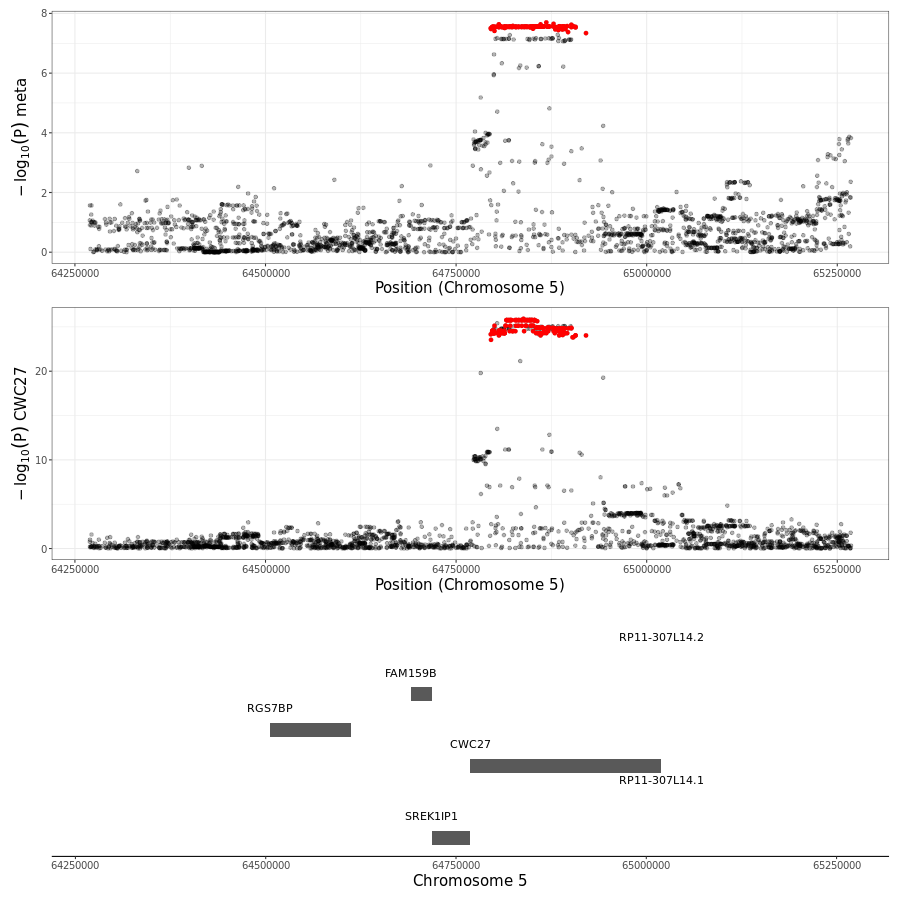
\includegraphics[width=1.0\textwidth]{Vector/cwc27_testis.png}
    \caption[Figure]{Regional association plot for the pAD-associated signal at index variant 5:64868326\_TTTC\_T(top) and \textit{CWC27} eQTL in testis (middle), showing position on the x-axis and $-log_{10}$ (P-value) on the y-axis. Red dots show pAD-associated genome-wide significant variants. Protein-coding and lincRNA gene positions are also shown (bottom).}
    \label{fig:cwc27_testis}
    \end{figure}





\section{Discussion}
In this chapter, I have performed several analysis to map genetic variants associated with perianal disease (pAD), defined as anal and rectal fissures and fistulas. I have leveraged two large-scale national biobanks, UKBB and FinnGen, with a total of 11,216 cases and 585,420 controls. First, I performed a separate UKBB GWAS and found seven genome-wide significant loci, that I subjected to a number of post-GWAS quality checks to ensure their veracity. Next, I downloaded FinnGen GWAS summary statistics for the same phenotype and performed similar post-GWAS quality checks. I also attempted to cross-replicate each GWAS' findings, and found that three of the seven UKBB loci replicated in FinnGen, while all FinnGen loci replicated in the UKBB. Interestingly, all the UKBB loci that failed to replicate in FinnGen were located in the MHC region, which is known to be highly polymorphic and exhibits complex LD patterns that tend to be population-specific. \\

There are several possible explanations for the absence of replication at the MHC loci. First, it is possible that neither the index variants nor their LD friends tag the true causal variant in FE. This is likely to be the case for the MHC loci where the index variant tags several LD friends, but none of them pass the replication P-value threshold. Second, a lack of statistical power might lead to an absence of replication, especially given the heterogeneity in pAD cases. The UKBB pAD case cohort is composed of perianal fissure and fistula cases, with fistulas representing 37.7\% of the pAD cases and it is unclear whether the FinnGen case cohort composition is similar. Third, the four MHC loci found in the UKBB may simply be spurious associations due to cryptic subpopulation stratification within the UKBB. As I showed in Section \ref{sec:ukbb_postgwas}, association strength and LD were not correlated in at least two of the MHC loci, which suggests that the true underlying LD does not match general population LD and may lead to spurious associations at these loci. \\

In order to maximise power to detect more genome-wide association signals, I then performed a fixed effects meta-analysis between the two GWAS. FinnGen and UKBB are derived from two different populations, with different LD structures, and therefore any genome-wide significant loci need to be carefully assessed to ensure they conform that the association strength conforms to both constitutent populations. Following this check, I found 12 genome-wide significant loci, two of which were located in the MHC region. Additionally, none of the index variants at these loci showed evidence of heterogeneity of effects between the two cohrots.\\

Despite the increased power afforded by meta-analysis, several limitations should be noted. First, a large proportion of the variants used in the meta-analysis (31\%) were either not genotyped/imputed or did not pass genotype or imputation QC in one of the two GWAS. This heterogeneity may bias which variants achieve genome-widen significant association, and may have led to missing several genome-wide significant hits. Second, pAD definition is based on a relatively broad ICD-10 code and a broad FinnGen endpoint that encompasses acute and chronic fissures and fistulas. The contribution of each of these subphenotypes to the genome-wide significant signals is not obvious. In this study, I was limited by the restricted access to individual-level FinnGen data, but future work should focus on assessing the contribution of each of the pAD subtypes to each genome-wide significant locus. \\

Following up on the meta-analysis results, I prioritised two follow-up analyses to better characterise the effects of the 12 pAD-associated loci. I observed that pAD cases are highly enriched in haemorrhoids compared to pAD controls (38\% versus 6\% respectively), which may suggest that there may be shared genetic effects underlying both pAD and haemorrhoids. I therefore performed an analysis where I disentangled the effects of the pAD-associated variants on both diseases. This analysis showed that the effects of these variants were stronger and more significant on pAD than haemorrhoids despite a large difference in statistical power. However, this analysis was limited to UKBB participant, and it is plausible that better powered GWAS of haemorrhoids may reveal that a larger proportion of the 12 pAD-associated variants are also associated with haemorrhoids. Indeed, when I replicated the index variants in Zheng et al. \cite{Zheng2021-ss}, I found that six of the 12 variants showed genome-wide significant association (P-value < $5\times10^{-8}$). However, similar to the UKBB analysis, they all had a concordant but smaller effect sizes on haemorrhoids than pAD. A compelling interpretation of this shared genetic risk is that pAD may be a more severe form or manifestation of haemorrhoids, with the same genetic variants underlying both and with stronger effect sizes on pAD. But this interpretation does not take account of the limited nature of a targeted genetic association test. Over 100 haemorrhoids associated loci were identified by Zheng et al., and it is plausible that most of these loci will not be associated with pAD if a genome-wide significant comparison was performed between the two diseases. Therefore, any conclusions made regarding the difference in effect sizes should be limited to these 12 loci.\\

Finally, I aimed to identify effector genes at each locus using colocalisation analysis. Although I identified several genes that colocalised with high confidence, evidence at most loci was conflicting, implicating several genes in several tissues. The role of these genes in many of the tissues where the colocalistions were detected, such as testis, thyroid and liver, was difficult to interpret given our knowledge of the pathogenesis of pAD. Although I showed evidence that two of these genes, \textit{LFNG} and \textit{CWC27}, were necessary for normal skeletal development, this does not constitute sufficient evidence for a novel insight into pAD pathogenesis. To this end, more follow-up work should be conducted to better interpret these loci. First, more robust methods need to be employed to establish a causal link between these loci and effector genes (e.g. Mendelian Randomisation methods \cite{Sanderson2022-nm}). Additionally, QTL studies from more relevant tissues need to be used. As discussed in \ref{sec:coloc}, it is well-known that genetic variants affect the expression of different genes in different tissues. Therefore, QTLs derived from anorectal tissues will provide the best colocalisation and mendelian randomisation evidence for effector genes. In conclusion, establishing a bona fide set of effector genes for these loci in relevant tissues will provide much stronger evidence that points to biological pathways implicated by pAD loci effector genes. 

% %!TEX root = ../thesis.tex
%*******************************************************************************
%****************************** Fourth Chapter **********************************
%*******************************************************************************

\chapter{Epidemiological and genetic characterisation of perianal Crohn's Disease}

% **************************** Define Graphics Path **************************
\ifpdf
    \graphicspath{{Chapter4/Figs/Raster/}{Chapter4/Figs/PDF/}{Chapter4/Figs/}}
\else
    \graphicspath{{Chapter4/Figs/Vector/}{Chapter4/Figs/}}
\fi
\section{Contributions}
Genotype and imputation quality control was performed by Dr. Laura Fachal and kinship analysis was performed by Dr. Marcus Tutert as part of the ongoing International IBD Genetics Consrtium GWAS project that is being undertaken in the Anderson laboratory. HLA allele imputation was performed by Dr. Qian Zhang as part of his IBD-BR drug response and disease progression study. I performed all the GWAS analyses, meta-analyses and all downstream analyses described in this chapter.
\section{Introduction}
Perianal Crohn's disease (pCD) is a sub-phenotype of Crohn's disease, a chronic inflammatory disease of the gut that affects 1\% of the population worldwide. pCD represents a major burden on both patients and healthcare providers, and is estimated to affect 20-40\% of CD patients worldwide, with a higher prevalence in Asia than in Western countries \cite{Ng2016-al}. As their disease progresses, CD patients become more likely to develop perianal symptoms. Twenty years after their CD diagnosis, CD patients have a 32\% cumulative probability of developing pCD \cite{Brochard2022-hx}. Timing of pCD diagnosis, however, varies significantly between healthcare systems. Previous studies from countries including France, Sweden and Japan have reported that between 4\%-68\% of pCD patients present with perianal symptoms before or at the time of CD diagnosis \cite{Mizushima2021-hk,Pogacnik2019-aj,Wils2021-ao}.\\

\subsubsection{Clinical picture of pCD}
pCD patients present with a variety of perianal symptoms. These include perianal skin tags, fissures, ulcers, faecal incontinence, rectal discharge and bleeding, perianal abscess, and fistulas. Perianal fistulas are the most common form of pCD, followed by perianal abscess \cite{Eglinton2012-vx}. Likewise, the impact of pCD on patients is multi-faceted. In addition to physical manifestations, patients report impaired quality of life as well as social and emotional complications of pCD. Furthermore, surgical interventions that aim to treat pCD and restore normal ano-rectal functions, such as seton insertion and fistula drainage, often impact essential functions such as walking and sitting \cite{Adegbola2020-nd}. Moreover, pCD patients, who often require multiple surgical interventions, suffer from high recurrence and relapse rates of pCD. In fact, only one third of pCD patients are estimated to achieve remission \cite{Panes2018-su,Braithwaite2017-zo}. \\

% To inform clinical decision making, several clinical scoring systems have been proposed to describe the clinical picture and predict prognosis of pCD. The first pCD scoring system was published by Hughes in 1992 \cite{Hughes1992-kc}. Hughes classified pCD lesions into primary lesions, such as fissures and ulcers, and secondary lesions such as skin tags, abscess and fistulas \cite{Safar2007-dk}. A numeric score was given based on the presence and severity of ulcerations, fistulas or abscess, and strictures. However, this classification has had limited impact on clinical practice \cite{Scheurlen2023-gk}. The Perianal Disease Activity Index is the  (PDAI), which has been devised to predict surgical outcomes in pCD patients, is the most widely used measure of pCD activity. PDAI scores six pCD clinical indicators on a Likert score: abscess, fistula, fissure and ulcer, stenosis, incontinence, and concomitant disease. Patients with no perianal involvement score 0 and patients with advanced perianal disease score a maximum of 55  \cite{Pikarsky2002-gf}. Compared to other clinical scoring systems, PDAI correlates well with pCD outcome and has been recommended for use in clinical practice \cite{Irvine1995-ej}.\\

Despite the diversity in presentation and course, pCD patients share a number of Crohn's disease characteristics. pCD is  more common among patients with more distal than proximal disease, and patients with colonic or rectal CD are more likely to develop or initially present with pCD. Moreover, pCD tends to drive Crohn's disease towards a more invasive behaviour. Initially, two thirds of patients have inflammatory manifestations, but over time, the majority of pCD patients display increasingly stricturing and penetrative characteristics of CD \cite{Peyrin-Biroulet2010-mf,Scharl2017-sp}, which are characterised by a narrowing of the lumen, and development of abdominal fistulas, inflammatory masses and abscess \cite{Gasche2000-qh}.  However, invasive distal CD does not always precede pCD, which can sometimes present a diagnostic challenge in clinical settings. Although 95\% of patients will eventually develop luminal disease, an estimated 17.2\% of patients initially present with pCD only \cite{Eglinton2012-hh}. \\


\subsubsection{Pathogenesis of pCD}
At a more fundamental level, our biological understanding of pCD fistula formation and progression mechanisms is still markedly lacking. One proposed pathophysiological mechanism is epithelial-to-mesenchymal transformation (EMT). EMT is a well-studied biological process, whereby polarised epithelial cells gain mesenchymal functions, such as enhanced cell invasion, and migration (reviewed in \cite{Kalluri2009-uu}). The EMT hypothesis is supported by the presence of transitional cells which express both epithelial and mesenchymal cell markers in fistula tracts. These include epithelial markers cytokeratin 8 and 20, and mesenchymal markers vimentin and actin. Transforming growth factor $\beta$ and interleukin-13, which have been associated with the initiation of EMT, have also been identified in transitional cells lining pCD fistula tracts \cite{Scharl2013-uf,Bataille2008-ej,Bataille2004-vf}. Despite these observations, little is understood about the causal biology of pCD. What are the drivers of this transformation? What causes variation in fistulising disease severity? Which biological pathways give rise to fistulas and what facilitates their development into complex branching structures? What is the role of genetic variation in pCD predisposition? In this regard, genome-wide association studies have improved our understanding of the pathophysiology of several complex disease \cite{Cano-Gamez2020-nm}. In the case of pCD, a well-powered GWAS between CD patients who develop pCD and CD patients who do not can help us understand which effector genes and biological pathways are causally linked to pCD risk. Unfortunately, none of the pCD GWAS conducted so far were able to identify genome-wide significant variants associated with pCD risk. Some studies have investigated nominally significant association to better understand pCD biology, but the hypotheses about causal biology remain difficult to reconcile. For example, based on a GWAS of 1,720 CD patients with and without pCD, Kaur et al. \cite{Kaur2016-bs} report an enrichment of nominally-associated variants in genes implicated in the JAK/STAT pathway, a proinflammatory signalling cascade that has previously been implicated in several autoimmune diseases \cite{Hu2021-us,Seif2017-bk}. More recently, Akhlaghpour et al. \cite{Akhlaghpour2023-jw} found a nominally-associated coding variant that impaired macrophage phagocytosis, and hypothesised that it may contribute to the pathogenesis of fistulising pCD. But overall, there is no clear consensus on the genetic underpinnings of pCD risk.\\

\subsubsection{Available pCD cohorts}
The NIHR IBD-BR is a UK-wide collaborative project that is part of the NIHR Bioresource, with the aim of recruiting 50,000 patients with Crohn's disease, ulcerative colitis or unclassified IBD. The IBD-BR collects phenotypic and epidemiological information (both clinical and self-reported) as well as DNA samples for both array genotyping and whole-genome and whole-exome sequencing. The aims of the IBD-BR are wide-ranging. These aims include understanding the genetics of IBD response to therapy, disease mechanism as well as determinants of disease course \cite{ibdbr-protocol-v8,ibdbr-questionnaire-v7,ibdbr-further-info}. So far, the IBD-BR has recruited over 31,000 patients, with epidemiological characteristics, clinical phenotypes, extra-intestinal manifestations, prescribed medications and treatment history, surgical history and disease behaviour and complications. The recruitment process starts by an expression of interest by volunteers who visit participating recruitment centres. Interested volunteers are then provided with an invitation letter and a patient information sheet that provides information on study requirements. Patients who agree to take part are then provided with an informed consent form, and subsequently asked to complete a health and lifestyle questionnaire. After these initial steps, the clinical team then proceeds to collect clinical data from hospital records. A clinician or research nurse extracts core information including IBD type, location and behaviour, complications, comorbidities, family history, smoking history, surgical data and
drug therapy outcomes \cite{ibdbr-protocol-v8}. Disease location data include details of perianal manifestations, which can be used to define a pCD case-control cohort.\\

Another pCD case control cohort can be defined using data from The UK IBD Genetics Consortium (UKIBDGC), a large collaborative consortium that studies the genetics of IBD susceptibility, progression and drug response. Patients are recruited from multiple UK centres in Cambridge, Edinburgh, Manchester, Newcastle, Exeter, Oxford, London, Dundee and Nottingham, and other sites across the UKB \cite{ukibdgc-info}. In additiona to basic epidemiological data such as sex, age, smoking and family history, data on type of IBD, location, surgery, and extraintestinal manifestations is recorded. Disease location data also include whether the disease is located in the perianal region.\\

Although data on perianal disease are recorded for both cohorts, the depth of clinical phenotyping is different. For example, the IBD-BR, contains information about specific manifestations of pCD. Clinicians and clinical nurses who complete the IBD-BR questionnaire perform an automated search of hospital records for clinical IBD information, including perianal manifestations \cite{ibdbr-protocol-v8}.  If the search is unsuccessful, they ask patients about perianal involvement: \textit{"Ever had perianal involvement? 1) Yes 2) No 3) Unknown"}  and record the answer in the clinical questionnaire \cite{ibdbr-questionnaire-v7}. A follow-up question about the type of perianal involvement is then asked: \textit{“If Yes - What type of perianal lesion has the patient had? (Select all that apply): 1) Tags/fissures/ulcers 2) Perianal abscess 3) Simple fistula 4) Complex fistula 5) Other”}. Clinicians may report one or more perianal involvement manifestations.  Unlike IBD-BR, the specific manifestations of pCD , such as fissures, ulcers or fistulas are not recorded for UKIBGC participants and only a binary phenotype is recorded (pCD+ or pCD-). \\

In this chapter, I describe several analyses I conducted to characterise pCD. Using the rich clinical phenotyping in the IBD-BR, I first explored the clinical characteristics of pCD+ patients, which largely conformed with what is known about the disease characteristics of pCD. Moreover, given our limited understanding of the genetic underpinnings of pCD \cite{Eglinton2012-ls,Latiano2009-bu,Tozer2009-mp,Akhlaghpour2023-jw,Kaur2016-bs}, I also performed a pCD GWAS meta-analysis leveraging the pCD cohorts of IBD-BR and UKIBDGC to identify pCD-associated variants. I conclude with an analysis that may partly explain the discovered pCD-associated hit and outline future steps for a more comprehensive understanding of the genetic underpinnings of pCD.
\section{Methods}
\subsection{pCD prevalence estimates}
IBD-BR patients were diagnosed with CD over several decades, mostly from 1980 till 2018. To investigate the temporal trends of pCD prevalence, I divided participants by year of CD diagnosis into 39 windows, and calculated pCD point prevalence in each two-year period. Additionally,to calculate 95\% confidence intervals around each point estimate, I randomly subsampled CD patients 1,000 times using a bootstrap proceducre implemented in the \Verb+boot()+ functions. Finally, I compared overall trends in prevalence estimate by pooling CD participants diagnosed with CD before and after 2010 and calculated point estimates and confidence intervals as mentioned before. The difference between these overall estimates was then tested using a t-test to deterime if pCD prevalence has significantly decreased before and after 2010.
\subsection{UK IBD Genetics Consortium Genotype Quality Control}
UKIBDGC samples were genotyped with two genotyping arrays: Affymetrix Human Mapping 500K Array (I will refer to this as GWAS1; number of variants before QC=469,281), and Illumina Human Core Exome-12v1.0 or its newer version Illumina Infinium Core Exome-24v1.1 (I will refer to this as HCE; number of variants before QC=535,434 and 557,662 respectively). Quality control for UKIBDGC genotype data was performed as part of the International IBD Genetics Consortium cases-control meta-analysis. QC was performed using a combination of Plink (v1.9 and v2), bcftools (v1.16), and KING (v2.2.4).
\subsection{Variant-level QC}
Variants that met the following criteria were excluded: 
\begin{itemize}
  \item Low call rate (< 0.95 for variants with minor allele frequency (MAF) $>$ 0.01 or $<$ 0.98 for variants with MAF $\leq$ 0.01).
  \item Significant difference in genotype call rate (P-value $< 10^{-4}$) between IBD cases and controls.
  \item Large allele frequency (AF) differences between UKIBDGC and Gnomad (Non-Finnish Europeans), or TOPMed (global) using the following formula:

$$\frac{(P_{1}-P_{0})^{2}}{(P_{1}+P_{0})(2-P_{1}-P_{0})} > \epsilon$$ 


where $\epsilon=0.025$ or $0.125$, for Gnomad and TOPmed respectively,  $P_{0}$ is the minor allele frequency (MAF) in Gnomad or TOPMed and $P_{1}$ is UKIBDGC MAF. This formula accounts for larger AF differences between UKIBDGC and population references in common than in low-frequency variants. The TOPMed global AF difference cutoff is higher to account for AF computed across diverse populations
\item Hardy Weinberg Equilibrium (HWE) P-value < $10^{-5}$ in IBD controls or < $10^{-12}$ in IBD cases.
 or 
\item Monomorphic variants. 
\end{itemize}

\subsection{Sample-level QC}
Samples that meet the following criteria were excluded:
\begin{itemize}
\item Missing genotyping rate $>$ 0.05
\item Heterozygosity estimate $\pm$ 4 standard deviations from the European-ancestry mean, or 
\item mismatch between recorded gender and genotypically-inferred sex. 
\end{itemize}
\subsection{Imputation to TOPMed}
The TOPMed imputation server (imputationserver at 1.5.7) was used for UKIBDGC genotype imputation. Alleles at directly genotyped variants with an empirical imputation $R < -0.5$ were flipped, and variants with empirical $R^{2} \leq 0.5$ were excluded after imputation. After their exclusion, imputation was repeated, and another HWE filtering step was performed.

\subsection{IBD-BR Genotype QC and Imputation}
The cohort was genotyped with two different versions of the UKBiobank ThermoFisher genotyping array. The same genotype QC steps as UKIBDGC were applied to IBD-BR, except for 1) The AF difference check, where 1000 Genomes Panel (1000GP) was used as a reference panel 2) Imputation, where the Sanger Imputation Server was used \cite{1000gp}, with two imputation reference panels: UK10K+1000GP and HRC. Imputed genotypes from both panels were combined. For variants that existed in both panels, HRC imputed genotypes were retained. 

Genotypic principal components (PC) were estimated for all participants, using a set of genotyped variants that were also available in the 1000 Genomes Project (100GP; excluding variants associated with IBD susceptibility; P-value < $10^{-4}$, and variants in long LD regions (as defined in \cite{plink_high_ld}). This final list was pruned with the following parameters: window size = 50 kbp; step size = 5; $R^{2}$ = 0.2. PCs were then projected to 1000GP PCs. Samples within the European ancestry group were retained for the subsequent analyses. 

\subsection{Identification of overlapping samples between UKIBDGC and IBD-BR}
Identification of duplicate individuals between UKIBDGC and IBD-BR genotyping data was performed with KING \cite{king-software}. Duplicates were defined as sample pairs with a kinship coefficient > 0.354 as recommended in KING documentations \cite{king-software}. Estimation of kinship coefficient was performed using post-QC genotyped SNPs (number of variants used for kinship inference between IBD-BR and GWAS1=42,292:, and between IBD-BR and HCE=53,431).

\subsection{Genome-wide association analysis}
All genome-wide association analyses were performed using REGENIE v3.2.5 \cite{Mbatchou2021-qm} following a 2-step approach. This approach is more computationally efficiency than other approaches that account for cryptic relatedness between individuals, such as linear mixed models. Briefly, in step 1, a whole-genome regression model is fitted using a subset of high-quality genome-wide variants in order to estimate a set of genome-wide predictors that capture a large fraction of phenotypic variance. These predictors are then included as covariates in the single-variant association models tested in step 2, where a larger set of variants of interest are tested for association. I used post-QC genotyped variants in step 1 as recommended by REGENIE documentation ($N_{IBD-BR}$=338,697; $N_{UKIBDGC(HCE)}$=359,209; $N_{UKIBDGC(GWAS1)}$=436,931), and both genotyped and imputed variants in step 2, testing all autosomal chromosomes ($N_{IBD-BR}$=9,777,139; $N_{UKIBDGC(HCE)}$=,916,200; $N_{UKIBDGC(GWAS1)}$=8,897,554). The step 2 model was specified as following: pCD $\sim$ variant + sex + genotypic PCs, using first 4 genotypic PCs. Step 2 reports single-variant association summary statistics. 

\subsection{Meta-analysis of IBD-BR and UKIBDGC cohorts}
I used METAL to perform the fixed-effects meta-analysis between the IBD-BR and UKIBDGC summary statistics.  METAL can perform fixed-effects meta-analysis using one of two different well-established schemes: P-values and effective sample size, or effect sizes and standard errors. The P-value scheme is implemented to enable meta-analysis of GWAS summary statistics that do not report the effect allele, while the effect sizes scheme can be used when each variant's effect size and effect allele are reported. All my pCD GWAS analyses report the effect allele, so I used the effect size scheme of METAL (\Verb+SCHEME STDERR+). \\

There was a total of 8,473,930 overlapping variants across the meta-analysed summary statistics, and an additional 1,645,123 variants that were unique to one of the studies, 42.7\% of which were indels. Given that 16\% of variants were unique to one of cohorts, I did not remove them from their respective summary statistics file. It is important to note, however, that this choice may favour variants that are available in all studies. 

\begin{table}[H]
  \caption{Number of SNPs and indels in each of the three GWAS summary statistics.}
  \centering
  \begin{tabular}[t]{lrrr}
  \toprule
  \textbf{Studies} & \textbf{SNP} & \textbf{Indel} & \textbf{Total}\\
  \midrule
  IBD-BR & 8,626,072 & 1,150,933 & 9,777,005\\
  UKIBDGC (GWAS1) & 8,307,857 & 589,198 & 8,897,055\\
  UKIBDGC (HCE) & 8,325,721 & 589,997 & 8,915,718\\
  \bottomrule
  \end{tabular}
  \end{table}

Moreover, METAL automatically aligns any variants that may be flipped between the meta-analysed summary statistics. METAL also enables filtering of variants to be meta-analysed based on their allele frequencies, which was not necessary since I previously filtered out variants with MAF < 0.01 in each summary statistics file. Finally, given the potential subpopulation stratification in the IBD-BR GWAS ($\lambda_{GC}$=1.08), I enabled a METAL option to correct genomic inflation before performing the meta-analysis (\Verb+GENOMICCONTROL ON+) as recommended in METAL's documentation website. There was no evidence of genomic inflation in the meta-analysed summary statistics ($\lambda_{GC}$=1.03).\\

For each variant, METAL outputs the effect allele, meta-analysed effect size, standard error, and P-values. After performing meta-analyses, it is important to compare the effect sizes between the meta-analysed cohorts. Comparison of both the direction and magnitude of effect sizes gives an indication on how similar the estimated effects of meta-analysed genetic variants are. To formally test this, I used Cochran's Q test of effect size heterogeneity implemented in METAL. Cochran's Q test asseses two or more effect size estimates and their corresponding standard errors and reports a $\chi^{2}$ statistic that quantifies the deviation from the null hypothesis that the meta-analysed effect sizes are similar. Depending on the number of meta-analysed studies (in this case 3), a P-value is derived from a theoretical $\chi^{2}$ distribution with $N-1$ degrees of freedom, where N is the number of meta-analysed studies (heterogeneity of effect P-value $P_{het}$). I used $P_{het}$ to test if the genome-wide significant variants demonstrate heterogeity of effect size between the meta-analysed cohorts. To account for multiple variants being tested, I set a Bonferroni-corrected P-value threshold for rejecting the null hypothesis (P-value < $\frac{0.05}{k}$, where $k$ is the number of variants tested).

% \subsection{Post-hoc power analysis of genome-wide significant variants}
% Power analysis was conducted to verify if genome-wide significant variants were expected given the meta-analysis sample size. I used the R package \Verb+genepwr+ v1.04 \cite{genepwr-docs} to calculate the power of the study to detect each genome-wide significant variant given each variant's effect size, the study sample size, and case proportion over a range of MAFs from 0.01 to 0.1, and assuming a significance level $\alpha < 5\times10^{-8}$.


\subsection{LD calculation from 1000GP}
Reference LD panels obtained from the 1000 Genomes Project High Coverage project \cite{1000gphc} were used in the post-GWAS check to study the relationship between LD and association strength at the genome-wide significant locus. $R^{2}$ values were calculated between the index variant and all variants in the locus. I downloaded VCFs from the 1000GP high coverage and used PLINK v1.9 to compute LD between all variants and the index variant in a 1mbp window. I used unrelated individuals with non-Finnish European ancestry (NFE; N=426). Relevant samples were included in the LD calculation using the following PLINK command:
\begin{verbatim}
  plink --r2 --keep EUR.samples --ld-window-r2 0 
\end{verbatim}

\subsection{$\chi^{2}$ comparison between different pCD definitions}
In order to compare association statistics from the pCD meta-analysis to meta-analyses performed using more severe pCD+ case criteria (all perianal manifestations, abscess and fistula only, fistula only and complex fistula only), I adjusted the broad-definition $\chi^{2}$ values using this formula:

 $$\chi^{2}_{Broad,n}=\frac{n}{N}\chi^{2}_{Broad}$$

where $n$ is the sample size of the meta-analysis being assessed, $\chi^{2}_{Broad}$ is the broad-definition observed association statistic and  $\chi^{2}_{Broad,n}$ is the broad-definition association statistic adjusted for sample size. This adjustment ensure that comparison of association statistics from meta-analyses with different sample sizes is valid.

%From script:
%/nfs/users/nfs_o/oe2/ibdbr/scripts/hla/cond_meta.R

\subsection{HLA allele imputation}
HLA genes located in the major histocompatibility complex region (MHC) are known to contribute to immune disease susceptibility \cite{Shiina2009-wt}. Although sequence-based typing (SBT) is the gold standard to identify HLA alleles, its relatively higher cost and the complexity of HLA sequencing has prevented scaling up of SBT methods to large cohorts \cite{Beksac2014-gm}. HLA allele imputation methods based on SNP arrays are a reliable alternative to SBT methods of HLA typing, and can be performed using a small number of genotyped SNPs in each HLA gene \cite{De_Bakker2006-ho,Monsuur2008-fk,Jia2013-mh,Zheng2014-mj,Cook2021-px,Naito2021-jl} (reviewed in \cite{Naito2022-qy}). \\

HLA alleles were imputed for all IBD-BR and UKIBDGC individuals using HIBAG, a computationally efficient prediction algorithm that was pre-trained on a diverse set of haplotypes from different ancestries and is used to impute HLA alleles \cite{Zheng2014-mj}. Model parameters that were pre-trained on SNPs from the UK Biobank Affymetrix Axiom array from European and multi-ethnic ancestries were used in HLA imputation (downloaded from \cite{hibag-models-docs}). After downloading the pre-trained models, HLA imputation was performed at the HLA allele and HLA allele group levels  for a total of 7 HLA genes (4-digit and 2-digit resolutions; Table \ref{table:hla_allele_num}). 

\begin{table}[H]
  \centering
  \caption{Number of genotyped variants used to perform HLA imputation.}
  \label{table:hla_allele_num}
  \begin{tabular}{|l|l|l|}
  \hline
  Gene     & 2 digits & 4 digits \\ \hline
  HLA*A    & 723      & 717      \\ \hline
  HLA*B    & 763      & 752      \\ \hline
  HLA*C    & 819      & 770      \\ \hline
  HLA*DPB1 & 478      & 478      \\ \hline
  HLA*DQA1 & 753      & 655      \\ \hline
  HLA*DQB1 & 754      & 702      \\ \hline
  HLA*DRB1 & 675      & 653      \\ \hline
  \end{tabular}
  \end{table}
For each HLA allele, I performed the association test using the logistic regression model: pcd status $\sim$ HLA allele copies + covariates, with the R function \Verb+glm(family=binomial())+ and using the same covariates as used in the GWAS. The association analysis were performed separately for each of IBD-BR, UKIBDGC (HCE) and UKIBDGC (GWAS1). The association effect sizes and standard errors were subsequently meta-analysed using the R package \Verb+metafor+. Additionally, I performed conditional association analysis to investigate if any HLA alleles can account for genome-wide significant SNPs. Conditional association analyses were performed by including SNP dosages as covariates in the same model. 
% \subsection{First subsection in the first section}
% \dots and some more 

% \subsection{Second subsection in the first section}
% \dots and some more \dots

% \subsubsection{First subsub section in the second subsection}
% \dots and some more in the first subsub section otherwise it all looks the same
% doesn't it? well we can add some text to it \dots

% \subsection{Third subsection in the first section}
% \dots and some more \dots

% \subsubsection{First subsub section in the third subsection}
% \dots and some more in the first subsub section otherwise it all looks the same
% doesn't it? well we can add some text to it and some more and some more and
% some more and some more and some more and some more and some more \dots

% \subsubsection{Second subsub section in the third subsection}
% \dots and some more in the first subsub section otherwise it all looks the same
% doesn't it? well we can add some text to it \dots

\section{Results}
Among 30,894 IBD-BR participants, 15,152 were diagnosed with Crohn's disease, 14,819 of which had perianal involvement data: 4,448 answered "\textit{Yes}" to “\textit{Ever had perianal involvement?}” (pCD+; 30\%), 9,751 answered "\textit{No}" (pCD-; 65.8\%), and 620 answered “\textit{Unknown}” (4.1\%), matching previous pCD prevalence estimates. Perianal simple or complex fistula was the most common manifestation (2327;  52.3\% pCD+ participants), followed by perianal abscess (1806; 40.5\% of pCD+ participants).

From 26,327 UKIBDGC patients, a total of 8,977 were diagnosed with CD. 7106 CD patients had perianal involvement information. pCD prevalence was lower than IBD-BR. 18.2\% of CD patients reported perianal disease location, 61\% reported a different disease location, and 20.8\% answered "\textit{Unknown}". UKIBDGC does not report specific manifestations of pCD.

\subsection{Epidemiological characteristics}
Epidemiological characteristics of pCD+ and pCD- patients were largely similar in both cohorts (Table \ref{table:epidem}). Males were more likely than females to report perianal involvement in both cohorts (P-value={$7\times10^{-4}$} and {$8\times10^{-6}$} in IBD-BR and UKIBDGC respectively). pCD+ was not associated with a family history of CD, while smoking was slightly less common in pCD+ patients (P-value=0.006 and 0.003).
\setlength{\tabcolsep}{10pt} 
\renewcommand{\arraystretch}{1.5}
\begin{table}[H]
  \caption{Epidemiological characteristics of pCD+ and pCD- patients in IBD-BR and UKIBDGC}
  \label{table:epidem}
  \centering
  \begin{tabular}[t]{lllll}
  \toprule
  \multicolumn{1}{c}{ } & \multicolumn{2}{c}{IBD-BR} & \multicolumn{2}{c}{UKIBDGC} \\
  \cmidrule(l{3pt}r{3pt}){2-3} \cmidrule(l{3pt}r{3pt}){4-5}
   & pCD+ & pCD- & pCD+ & pCD-\\
  \midrule
  Male & 2115 (47.5) & 4339 (44.5) & 807 (49.5) & 2363 (43.2)\\
  Female & 2333 (52.5) & 5412 (55.5) & 824 (50.5) & 3112 (56.8)\\
  Family History & 1325 (34.7) & 2795 (34.2) & 290 (27.1) & 598 (24.6)\\
  Surgery & 2971 (68.8) & 3636 (38.3) & 896 (63.1) & 1935 (42.6)\\
  Smoking & 656 (16.4) & 1572 (18.2) & 363 (30.1) & 913 (29.6)\\
  \bottomrule
  \end{tabular}
  \end{table}


  \subsection{Clinical characteristics}
\subsubsection{pCD is associated with lower age-of-CD-diagnosis and rectal CD}

Previous pCD studies have reported an association between pCD and distal penetrating CD, as well as pCD and an earlier age of CD diagnosis \cite{Duricova2014-gf,Kaur2016-bs}. Compared to pCD- patients, pCD+ patients were significantly younger at diagnosis (P-value < $2\times10^{-16}$; median age of CD diagnosis for pCD+ patients was 24 versus 29 for pCD- patients in IBD-BR; Figure \ref{fig:age_diag_macextent}). Additionally, pCD+ patients were at least twice as likely to have penetrating disease behaviour. In IBD-BR, 19.1\% of pCD+ patients had disease behaviour classified as B3 versus 8.1\% in pCD-. This enrichment was stronger in UKIBDGC (28.5\% versus 10.6\%, respectively). \\

In both cohorts, more patients reported ileal than colo-rectal CD (68.7\% versus 56.3\% in IBD-BR). Ileal and colo-rectal CD were either isolated, or extended to other parts of the gut. In IBD-BR, patients with an isolated colo-rectal CD were 2.4 times as likely to develop pCD, compared to patients with an isolated ileal CD (59.3\% versus 24.8\%).  Despite the lower pCD prevalence in UKIBDGC, patients with isolated colo-rectal CD were similarly enriched for pCD+ patients as IBD-BR (26.6\% versus 10.9\%). \\

In IBD-BR, where colonic and rectal involvement are reported as separate indicators, rectal involvement accounted for this enrichment. Patients with isolated colonic disease were not significantly more enriched for pCD+ than patients with isolated ileal disease (28.3\% versus 24.8\%; Figure \ref{fig:age_diag_macextent}).
\begin{figure}[htbp!] 
  \centering    
  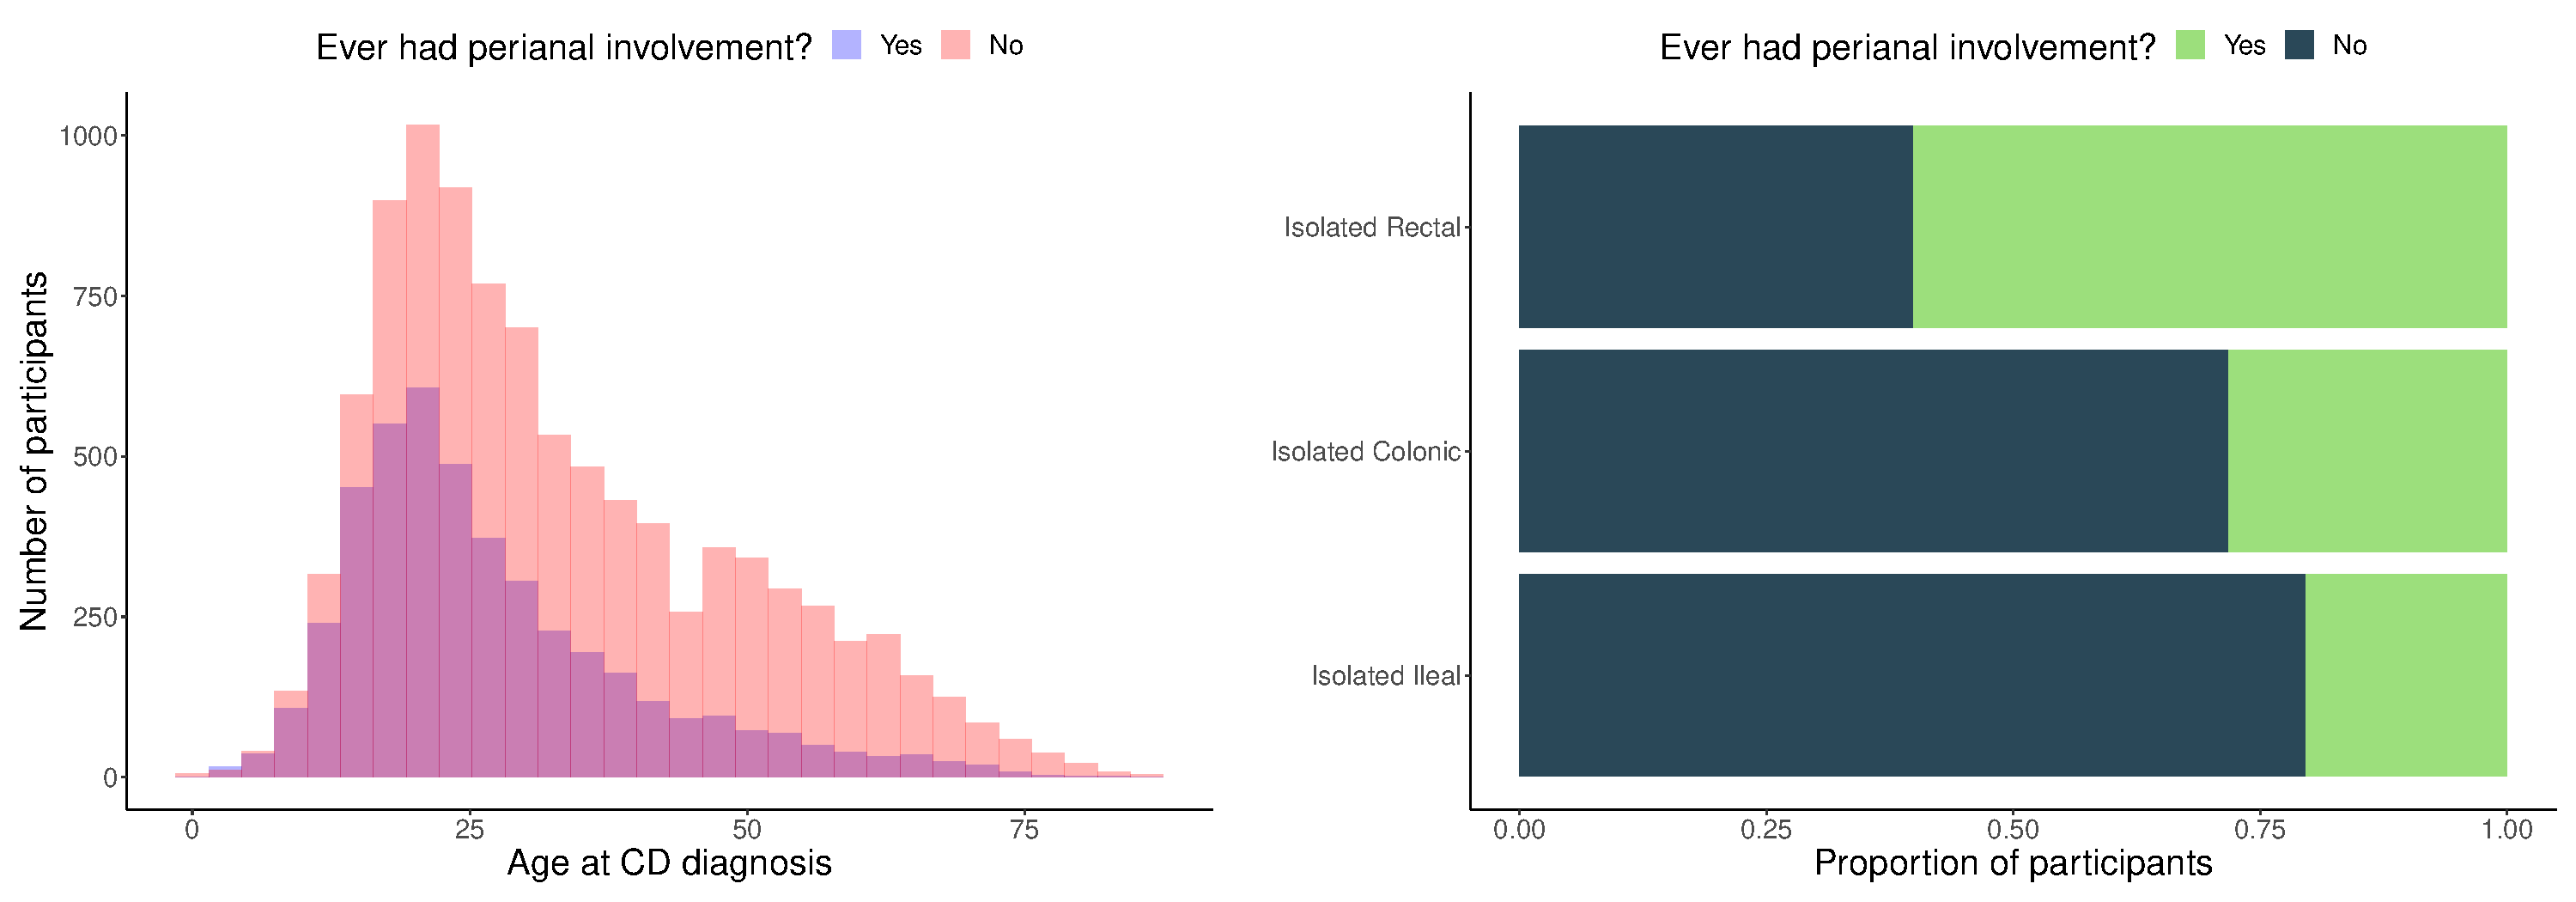
\includegraphics[width=1.0\textwidth]{fig1}
  \caption[Figure]{age at diagnosis and macroscopic extent of Crohn's disease in pCD+ and pCD- patients in the IBD-BR.}
  \label{fig:age_diag_macextent}
  \end{figure}

\subsubsection{Lower rates of drug intake in pCD+ patients in IBD-BR}
pCD+ patients were less likely to be actively prescribed a number of CD medications: oral steroids, Infliximab, Adalimumab, Vedolizumab, and Mesalazine (P-value $<$ 0.0036; Table \ref{table:drug_eim}; odds ratio=0.83, 0.77, 0.62 and 0.55 respectively). Anti-TNF therapies, including Infliximab and Adalimumab, are among the first-line drugs for perianal fistulas, and lead to fistula healing in 50\% of pCD patients (in combination with other surgical procedures) \cite{Regueiro2003-lf,Kotze2014-fh,Haennig2015-pj,Gaertner2007-wb}. Additionally, the ENTERPRISE clinical trial found that Vedolizumab achieved remarkable fistula closure and healing \cite{Schwartz2022-zp}. On the other hand, oral steroids are known to be ineffective for fistula closure and may even exacerbate perianal abscess \cite{Jones1966-tt}. Lower drug intake could therefore be attributed to drug inefficacy, but it could also be a contributing factor to pCD.\\

\subsubsection{pCD+ patients are enriched for six extraintestinal manifestations}
pCD+ patients were enriched for extra-intestinal manifestation compared to pCD- patients (26.3\% versus 19.6\%; P-value $<$ 0.05). Enteropathic arthritis was the most most prevalent extraintestinal manifestation among pCD+ patients, followed by serious infections and psoriasis. In total, six extraintestinal manifestations showed significant enrichment in pCD+ versus pCD- patients (P-value $<$ 0.005; Table  \ref{table:drug_eim}). The association between extraintestinal manifestations was stronger in female participants, possibly since extraintestinal manifestations were more prevalent in female participants overall (odds ratio=1.3 in males versus 1.6 in females). 
\begin{table}
  \centering
  \begin{tabular}[t]{llll}
  \toprule
  \textbf{} & \textbf{pCD+(\%)} & \textbf{pCD-(\%)} & \textbf{P-value}\\
  \midrule
  \addlinespace[0.3em]
  \multicolumn{4}{l}{\textbf{Extraintestinal Manifestations}}\\
  \hspace{1em}Primary Sclerosing Cholangitis & 25 (0.6) & 72 (0.8) & 0.29\\
  \hspace{1em}Enteropathic Arthritis & 413 (9.7) & 635 (6.7) & $2.1\times10^{-9}$\\
  \hspace{1em}Erythema Nodosum & 199 (4.6) & 222 (2.3) & $7.7\times10^{-13}$\\
  \hspace{1em}Iritis & 183 (4.2) & 242 (2.5) & $1.1\times10^{-7}$\\
  \hspace{1em}Orofacial Granulomatosis & 153 (3.6) & 162 (1.7) & $2.4\times10^{-11}$\\
  \hspace{1em}Psoriasis & 311 (7.2) & 518 (5.4) & $6\times10^{-5}$\\
  \hspace{1em}Ankylosing Spndylitis & 110 (2.6) & 238 (2.5) & 0.89\\
  \hspace{1em}Multiple Sclerosis & 9 (0.2) & 27 (0.3) & 0.53\\
  \hspace{1em}Lymphoma & 18 (0.4) & 36 (0.4) & 0.85\\
  \hspace{1em}Serious Infections & 320 (7.4) & 465 (4.9) & $3.2\times10^{-9}$\\
  \addlinespace[0.3em]
  \multicolumn{4}{l}{\textbf{Drugs}}\\
  \hspace{1em}Azathioprine & 1373 (41.4) & 2649 (42.1) & 0.49\\
  \hspace{1em}Mercaptopurine & 271 (35.6) & 564 (36.1) & 0.83\\
  \hspace{1em}Methotrexate & 192 (28.6) & 404 (35.4) & ${4\times10^{-3}}$\\
  \hspace{1em}Infliximab & 1207 (50.9) & 1622 (55.7) & $6\times10^{-4}$\\
  \hspace{1em}Adalimumab & 740 (47.8) & 1368 (54.2) & $8\times10^{5}$\\
  \hspace{1em}Vedolimumab & 236 (67.8) & 424 (77.4) & $2\times10^{-3}$\\
  \hspace{1em}Ustekinumab & 171 (69.2) & 209 (72.6) & 0.45\\
  \hspace{1em}Mesalazine & 528 (30) & 1649 (43.7) & $< 2.2\times10^{-16}$\\
  \hspace{1em}Oral Steroids & 304 (11.3) & 823 (14.2) & $3\times10^{-4}$\\
 
  \bottomrule
  \end{tabular}
  \caption{Drug intake and extraintestinal manifestations in pCD+ and pCD- patients in the IBD-BR. Percentage of patients are shown between parentheses. Significant differences between pCD+ and pCD- were assesed using a $\chi^{2}$ test and the P-value is shown in the last column.}
  \label{table:drug_eim}
  \end{table}
  
% \begin{table}[htbp!]
%   \centering
%   \begin{tabular}{|l|l|l|r|}
%   \hline
%   Drug          & pCD+        & pCD-        & \multicolumn{1}{l|}{P-value} \\ \hline
%   Aza           & 1373 (41.4) & 2649 (42.1) & 0.4932629                    \\ \hline
%   Merc          & 271 (35.6)  & 564 (36.1)  & 0.8335190                    \\ \hline
%   Metho         & 192 (28.6)  & 404 (35.4)  & 0.0036395                    \\ \hline
%   Inflix        & 1207 (50.9) & 1622 (55.7) & 0.0006321                    \\ \hline
%   Ada           & 740 (47.8)  & 1368 (54.2) & 0.0000796                    \\ \hline
%   Goli          & 9 (56.2)    & 9 (50)      & 0.9838468                    \\ \hline
%   Vedo          & 236 (67.8)  & 424 (77.4)  & 0.0020198                    \\ \hline
%   Ust           & 171 (69.2)  & 209 (72.6)  & 0.4514008                    \\ \hline
%   Mesa          & 528 (30)    & 1649 (43.7) & 0.0000000                    \\ \hline
%   Oral\_ster    & 304 (11.3)  & 823 (14.2)  & 0.0002656                    \\ \hline
%   Other1\_treat & 195 (37.9)  & 434 (49.6)  & 0.0000318                    \\ \hline
%   Extraintestinal manifestations & pCD+      & pCD-      & \multicolumn{1}{l|}{P-value} \\ \hline
%   prim\_scler\_chol              & 25 (0.6)  & 72 (0.8)  & 0.2916513                    \\ \hline
%   enter\_arth                    & 413 (9.7) & 635 (6.7) & 0.0000000                    \\ \hline
%   ery\_nodo                      & 199 (4.6) & 222 (2.3) & 0.0000000                    \\ \hline
%   iritis                         & 183 (4.2) & 242 (2.5) & 0.0000001                    \\ \hline
%   oro\_gran                      & 153 (3.6) & 162 (1.7) & 0.0000000                    \\ \hline
%   psori                          & 311 (7.2) & 518 (5.4) & 0.0000596                    \\ \hline
%   ank\_spond                     & 110 (2.6) & 238 (2.5) & 0.8860326                    \\ \hline
%   mult\_scler                    & 9 (0.2)   & 27 (0.3)  & 0.5346415                    \\ \hline
%   lymphoma                       & 18 (0.4)  & 36 (0.4)  & 0.8479312                    \\ \hline
%   ser\_infect                    & 320 (7.4) & 465 (4.9) & 0.0000000                    \\ \hline
%   \end{tabular}
%   \end{table}
  % \begin{table}[]
  %   \centering
  %   \begin{tabular}{|l|l|l|r|}
  %   \hline
  %   Extraintestinal manifestations & pCD+      & pCD-      & \multicolumn{1}{l|}{P-value} \\ \hline
  %   prim\_scler\_chol              & 25 (0.6)  & 72 (0.8)  & 0.2916513                    \\ \hline
  %   enter\_arth                    & 413 (9.7) & 635 (6.7) & 0.0000000                    \\ \hline
  %   ery\_nodo                      & 199 (4.6) & 222 (2.3) & 0.0000000                    \\ \hline
  %   iritis                         & 183 (4.2) & 242 (2.5) & 0.0000001                    \\ \hline
  %   oro\_gran                      & 153 (3.6) & 162 (1.7) & 0.0000000                    \\ \hline
  %   psori                          & 311 (7.2) & 518 (5.4) & 0.0000596                    \\ \hline
  %   ank\_spond                     & 110 (2.6) & 238 (2.5) & 0.8860326                    \\ \hline
  %   mult\_scler                    & 9 (0.2)   & 27 (0.3)  & 0.5346415                    \\ \hline
  %   lymphoma                       & 18 (0.4)  & 36 (0.4)  & 0.8479312                    \\ \hline
  %   ser\_infect                    & 320 (7.4) & 465 (4.9) & 0.0000000                    \\ \hline
  %   \end{tabular}
  %   \end{table}

% \subsubsection{pCD and extraintestinal manifestations: other factors to consider}
% Other factors that may underlie this enrichment include treatment with anti-TNFs such as Infliximab, which are effective in reducing extraintestinal manifestations. In the previous section, I showed that pCD+ patients in IBD-BR are less likely to be actively taking a number of drugs including Infliximab. Therefore, an important question is whether this enrichment is driven by true shared pathophysiology between pCD and extraintestinal manifestations, or if it is merely due to lower rates of Infliximab intake in pCD+ patients (as well as other drugs).\\

% This can be tested by assessing the enrichment of extraintestinal manifestations within subsets of patients stratified by drug intake (e.g. patients currently on Infliximab versus patients not on Infliximab). If stratifying by drug intake does not affect the enrichment, then t is unlikely to be driven by drug intake. 
% However, information on drug intake, pCD and extraintestinal manifestations were jointly available for a smaller set of IBD-BR participants (n=5,133-5,186) that did not exhibit an enrichment of extraintestinal manifestations in pCD+ versus pCD- patients. Therefore, these sets of participants cannot be used to make a conclusion about the effect of drug intake on the observed enrichment in participants with pCD information. 




    \subsubsection{Surgical burden of pCD}

    Combined surgical and medical interventions represent some of the few effective interventions available to pCD patients. Different surgical options are available to perianal disease patients depending on its anatomical features, complications and disease severity. Exploration under anaesthesia and seton insertion are the typical first-line management options, and further medical or surgical interventions are based on initial exploration \cite{Adegbola2018-ha}. As expected, 2,971 pCD patients (66.8\%) had undergone any type of surgical intervention compared to 3,637 (37.2\%) of pCD- participants. In total, almost half the pCD+ patients with operative history had undergone one of three pCD-related surgical procedures (1431 patients; 48.2\%): drainge of perianal abscess, insertion of seton, or drainage of fistula. Perianal abscess drainage was the most common: 808 pCD+ patients (27.2\% of surgically-operated patients) underwent at least one perianal abscess drainage operation, followed by insertion of a seton suture (744 pCD+ patients; 25\%), followed by perianal fistula repair operation (438 pCD+ patients; 14.7\%).

    \subsubsection{pCD prevalence decreased over time}
    Understanding pCD prevalence over time is important to understand how the burden of pCD on patients and healthcare providers has changed. Previous work has shown reduced pCD incidence over the last decade \cite{Park2019-kj}, which was partly attributed to improved treatment options. In this regard, IBD-BR offers a unique opportunity to assess this trend. Although the precise time of pCD development is not avaialble, the time between CD diagnosis and the last clinical review can be used to compare how pCD prevalence among CD patients has changed in different eras. Over 93\% of IBD-BR patients with pCD information were clinically re-assessed in or later than 2016, which reduces the bias introduced by potentially outdated clinical data. \\
    
    To investigate this trend in the IBD-BR, I partitioned participants according to their year of CD diagnosis into two-year groups (e.g. 2006-2008), and calculated prevalence estimates in each period. As expected, confidence intervals around the point estimates were larger in the years between 1980-2010 since fewer IBD-BR patients were diagnosed with CD in those years (100-230 participants per two years). This rose to 497-734 per two years in the years from 2010 to 2020.  Notably, point prevalence estimates decreased starting from the year 2010 onwards. The mean point prevalence between 1980 to 2010 decreased significantly from 35.9\% to 25.1\% between 2010 to 2020 (t-test P-value $<2\times10^{-16}$; Figure \ref{fig:pcd_prev}). The decrease in prevalence remained significant when mean point prevalence was calculated between 2010 to 2016 only (mean prevalence=26.8\%), between 2010 to 2014 only (mean prevalence=28.1\%), or between 2010 to 2012 (mean prevalence=29.4\%).\\
    \begin{figure}[htb] 
      \centering    
      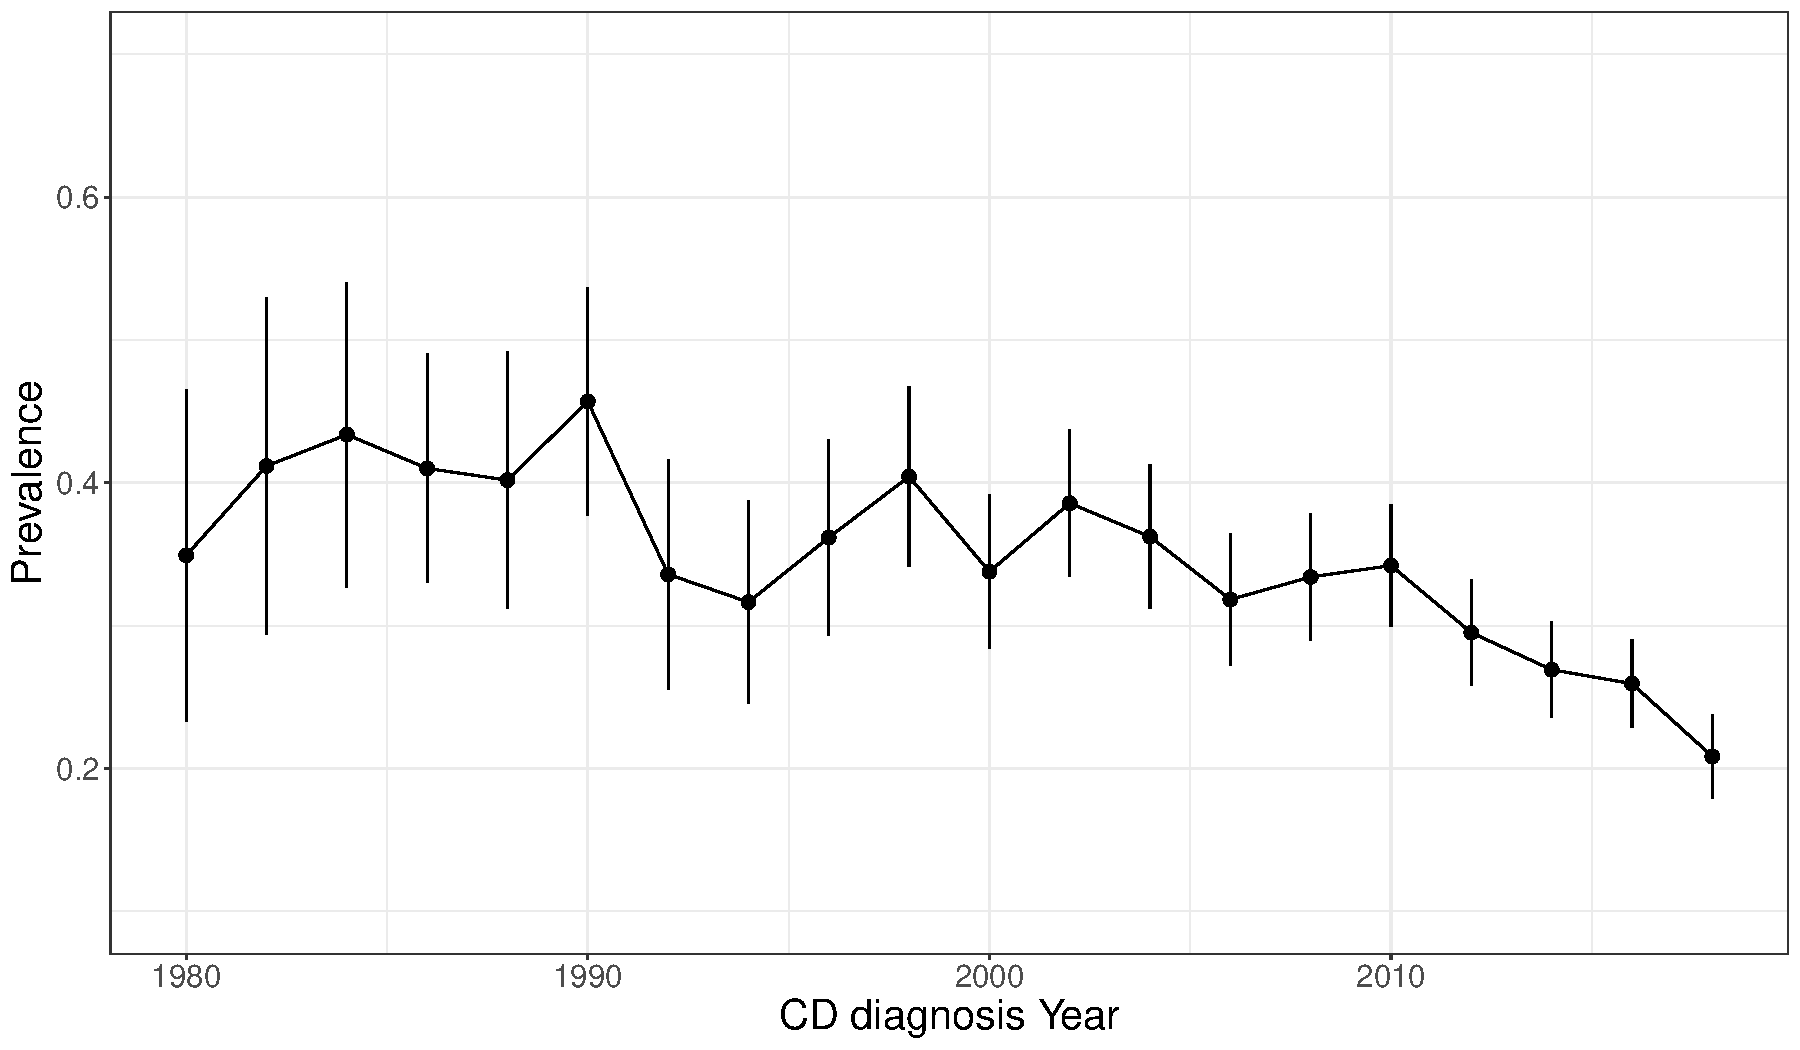
\includegraphics[width=1.0\textwidth]{fig2}
      \caption[Figure]{Prevalence per year of CD diagnosis, partitioned into two-year groups. 95\% confidence intervals around point estimates are calculated using a bootstrap procedure, whereby participants where resampled 1,000 times within each two-year group.}
      \label{fig:pcd_prev}
      \end{figure}
 
    A decrease in pCD prevalence has been observed previously \cite{Park2019-kj}. However, such a decrease has not been precisely quantified, partly due to the relatively smaller sample sizes of most studies \cite{Brochard2022-kz,Bruckner2018-ag,Gottgens2017-df,Tsai2022-kz}. A potential limitation of this analysis is that censored data may contribute to the observed decrease in pCD prevalence in later years. pCD does not always present at the time of diagnosis, which may bias prevalence estimates downwards in the years after 2010. An important consideration when investigating the effect of data censorship is that pCD prevalence estimates should be up-to-date. For example, a patient who is diagnosed with CD in 2012 for example may be incorrectly considered pCD-free if their clinical information were not updated afterwards. In IBD-BR, this bias is mitigated by the the fact that the majority of patients were clinically assessed between 2016 and 2021. Additionally, the consistent decrease in pCD prevalence even when I excluded patients diagnosed after 2016, 2014, or 2012 indicates that the contribution of censored observation is likely minimal. Although some patients may develop perianal symptoms up to 20 years after diagnosis, the cumulative probability of developing pCD does not increase significantly after 5 years \cite{Tsai2022-kz}. It is therefore unlikely that the decrease in pCD prevalence is affected by censored observations.

    \subsection{UKIBDGC and IBD-BR definitions of pCD are similar}
    Similar to IBD-BR, the UKIBDGC can be used to define a pCD+/pCD- cohort. The UKIBDGC reports a number of clinical and phenotypic characteristics of IBD patients. For each IBD participant, disease subtype diagnosis, and location (inclduding perianal disease) are recorded. However, it is unclear whether the criteria for assigning pCD status is consistent between the different centers, and more importantly if it matches the criteria used to assign pCD status to IBD-BR patients. Heterogeneity in pCD status definition can often arise from different diagnostic criteria being applied, or different times of phenotype update between patients. Ensuring the consistency of pCD status between UKIBDGC and IBD-BR is crucial to minimise the heterogeneity of phenotype definition between the two cohorts and maximise the statistical power from a meta-analysis between the two cohorts. 
To assess this, participants who may have taken part in both the IBD-BR and UKIBDGC can be leveraged to understand the level of agreement in pCD status assignment. Since participant identifiers are not mapped across studies, genetic similarity of individuals across cohorts can instead be leveraged to identify overlapping participants (Methods).\\

Out of 971 overlapping CD participants, only one participant exhibited discordant pCD status between IBD-BR and UKIBDGC. A total of 432 participants had missing or “Unknown” perianal involvement, 406 of which were“Unknown” in both cohorts (Table \ref{table:cohort_pcd_agree}). This strong agreement in pCD status indicates that both cohorts assign pCD status in a similar fashion.\\

I then asked if the UKIBDGC cohort was enriched for particular perianal manifestations. Since this information is not available in the UKIBDGC phenotype data, it can be obtained from the IBD-BR clinical data for patients who reported pCD+ status in both studies. I found that these patients were not enriched in any particular type of perianal involvement (e.g. 51.9\% of overlapping individuals reported either simple or complex fistula versus 52\% in IBD-BR). Moreover, 27\% of the overlapping patients reported only skin tags, fissures or ulcer, indicating that milder forms of pCD were also included in the UKIBDGC assignment of pCD+ status. Overall, this shows that the definition of pCD status is likely consistent between the cohorts. From the analysis of overlapping individuals it does not appear that the UKIBDGC pCD status assignment criteria were different from the criteria used in the IBD-BR questionnaire.


\begin{table}[htb]
  \caption{Number of overlapping individuals between UKIBDGC and IBD-BR who answered Yes, No or Unknown to \textit{Ever had perianal involvement?}}
  \label{table:cohort_pcd_agree}
  \centering
  \begin{tabular}[t]{|l|r|r|r|}
  \hline
  \multicolumn{1}{|c|}{ } & \multicolumn{3}{c|}{UKIBDGC} \\
  \cline{2-4}
  IBD-BR& Yes & No & Unknown\\
  \hline
  Yes & 201 & 0 & 1\\
  \hline
  No & 1 & 337 & 6\\
  \hline
  Unknown & 6 & 13 & 406\\
  \hline
  \end{tabular}
  \end{table}

  \section{Genome-wide association analysis of pCD}
  \subsection{Defining pCD+ cases}
  Genome-wide studies of disease subphenotypes pose unique challenges compared to traditional case-control GWASes. Unlike GWASes of CD, for example, where robust diagnostic criteria are applied to clearly demarcate cases and controls, in GWAS of disease subphenotype such as pCD it is not obvious which specific manifestations should be considered cases. The IBD-BR questionnaire reports several types of pCD manifestations, including skin tags, fissures or ulcers, perianal abscess, and simple and complex fistulas. In this chapter, my aim is to perform a pCD meta-analysis between IBD-BR and UKIBDGC, and therefore similarity in pCD+ case definition across the cohorts is an important consideration to ensure the robustness of genome-wide significant hits. In the previous section, I showed that leveraging individuals who registered for both studies can give an insight into the composition of the UKIBDGC pCD+ cases. This showed that UKIBDGC pCD+ cases were not particularly enriched in any particular type of perianal manifestations. Additionally, when I inspected the UKIBDGC questionnaire used to collect perianal manifestations data, I found that the relevant question appeared to include all types of perianal manifestations: \textit{"Ever had perianal fistula (incl recto-vaginal),  abscess, anal ulcer or significant anal stenosis?"}. I threfore defined pCD+ cases in both cohorts as CD patients that report any type of perianal involvement,
  
 
\subsection{IBD-BR}
Although clinical and phenotypic data are available for all participants, not all participants have been genotyped in the current release (04/04/2022). From a total of 15,152 participants with CD diagnosis, 9,458 European ancestry participants with perianal involvement data were genotyped. To ensure that pCD- controls do not include recently diagnosed CD patients who may develop perianal disease in the near future, I excluded pCD- controls diagnosed with CD less than 5 years before the last clinical review. This choice was informed by previous studies that showed that the cumulative risk of developing perianal disease 5 years and 10 years after diagnosis are similar \cite{Tsai2022-kz}. This resulted in a total of 6833 participants (2,664 pCD+ cases and 4,169 pCD- controls). After these filters were applied, the composition of genotyped pCD+ cases cohort matched the overall composition of all participants with perianal involvement information reported earlier. 53.6\% (1480) of genotyped pCD+ individuals had either a simple or complex perianal fistula, and 41.2\% (1098) had perianal abscess. Together, patients with perianal fistula or abscess account for 74.9\% (1995) of genotyped pCD+ cases.\\

With the pCD case-control cohort defined above, I performed GWAS between pCD+ cases and pCD- controls using REGENIE and used four European-ancestry genotypic principal components and sex as covariates. I removed variants with imputation INFO score < 0.4 and minor allele frequency (MAF) < 0.01, leaving 9,777,139 variants for association analysis (see Methods for detailed genotype and imputation QC). None of the tested variants achieved genome-wide significant association (P-value $< 5\times10^{-8}$). There was moderate evidence of genomic inflation (median $\chi^{2}$=0.49; $\lambda_{GC}$=1.08).
\subsection{UKIBDGC}
As mentioned earlier, UKIBDGC only reports whether or not partipcipants report perianal involvement and does not provide specific perianal manifestations. A total of 8,078 patients of European ancestry were diagnosed with CD, of which 6550 had perianal involvement information. To minimise sample overlap with the IBD-BR, I removed UKIBDGC individuals who showed genetic similarity with individuals from the IBD-BR (see Methods for more details on how genetic similarity was assessed), and performed GWAS with the remaining individuals (1303 pCD+ and 4761 pCD-). \\

I performed GWAS similar to the IBD-BR analysis, with the difference that UKIBDGC samples were genotyped with two different gentopying arrays and were therefore analysed seperately (I will refer to these two cohorts as HCE and GWAS1; Methods). A total of 8,916,200 and 8,897,554 variants were tested in HCE and GWAS1, respectively. No variants achieved genome-wide significant association (P-value < $5\times10^{-8}$). There was no evidence of genomic inflation (HCE: median $\chi^{2}$=0.47; $\lambda_{GC}$=1.04; GWAS1: median $\chi^{2}$=0.46; $\lambda_{GC}$=1.01).

\subsection{Meta-analysis between UKIBGC and IBD-BR: a genome-wide significant locus at 6p21.32}

I used METAL to perform a fixed-effects meta-analysis between summary statistics from IBD-BR, and the two UKIBDGC summary statistics HCE and GWAS1, with a total of 3,967 pCD+ cases and 8,930 pCD- controls. 
  Four variants in the MHC region at the 6p21.32 locus showed genome-wide significant association (index variant rs115378818; P-value=$8.6\times10^{-12}$; Table \ref{table:gws}). None of the variants showed significant heterogeneity of effect size between the constituent cohorts ($P_{het}$ < 0.008). All four variants were well-imputed across the constituent cohorts (INFO score > 0.7).
  \begin{table}[H]
    \caption{Genome-wide significant variants in the 6p21.32 locus. Odds ratio and their 95\% confidence intervals are shown. MAF=minor allele frequency.}
    \label{table:gws}
    \centering\begingroup\fontsize{10}{12}\selectfont
    
    \begin{tabular}[t]{|r|l|l|l|l|l|}
    \hline
    Chromosome & Position (b38) & Effect Allele & OR & P-value & MAF\\
    \hline
    6 & 32,205,822 & C & 1.45 (1.27 - 1.66) & $4\times10^{-8}$ & 0.05\\
    \hline
    6 & 32,243,461 & C & 1.38 (1.23 - 1.55) & $4.4\times10^{-8}$ & 0.08\\
    \hline
    6 & 32,279,268 & G & 1.57 (1.36 - 1.82) & $1.5\times10^{-9}$ & 0.05\\
    \hline
    6 & 32,333,650 & T & 1.78 (1.51 - 2.1) & $8.6\times10^{-12}$ & 0.04\\
    \hline
    \end{tabular}
    \endgroup{}
    \end{table}

    \begin{table}[H]

      \caption{\label{tab:table:maf_concord_cc}Case and control minor allele frequencies of the genome-wide significant variants in the 6p21.32 locus in all constituent cohorts.}
      \centering
      \fontsize{9}{11}\selectfont
      \begin{tabular}[t]{>{\raggedright\arraybackslash}p{5em}>{\raggedleft\arraybackslash}p{3em}>{\raggedleft\arraybackslash}p{3em}>{\raggedleft\arraybackslash}p{3em}>{\raggedleft\arraybackslash}p{3em}>{\raggedleft\arraybackslash}p{3em}>{\raggedleft\arraybackslash}p{3em}}
      \toprule
      \multicolumn{1}{c}{ } & \multicolumn{2}{c}{IBD-BR} & \multicolumn{2}{c}{UKIBDGC (HCE)} & \multicolumn{2}{c}{UKIBDGC (GWAS1)} \\
      \cmidrule(l{3pt}r{3pt}){2-3} \cmidrule(l{3pt}r{3pt}){4-5} \cmidrule(l{3pt}r{3pt}){6-7}
      SNP & Cases & Controls & Cases & Controls & Cases & Controls\\
      \midrule
      6:32333650\_C\_T & 0.042 & 0.027 & 0.059 & 0.037 & 0.055 & 0.035\\
      6:32279268\_T\_G & 0.054 & 0.038 & 0.067 & 0.046 & 0.062 & 0.044\\
      6:32205822\_T\_C & 0.063 & 0.046 & 0.070 & 0.051 & 0.065 & 0.047\\
      6:32243461\_G\_C & 0.084 & 0.066 & 0.092 & 0.073 & 0.099 & 0.072\\
      \bottomrule
      \end{tabular}
      \end{table}
%%%%%%%%%%%%%%%%%%%%%%%%%%%%%%%%%%%%%%%%%
%FIGURE SOURCE: /nfs/users/nfs_o/oe2/ibdbr/scripts/explore/manhattan.R
%%%%%%%%%%%%%%%%%%%%%%%%%%%%%%%%%%%%%%%%%

All four variants had a low minor allele frequency (MAF), ranging from  0.04 to 0.08 in the constituent cohorts (Table \ref{table:gws}). Low-frequency variant calling is more prone to genotyping errors than common variants, and therefore low-frequency genome-wide significant hits require additional quality checks. In some studies, these associations were later found to be false positives \cite{Tabangin2009-gs,Ayers2011-bc}. To minimise this risk and ensure the robustness of the associated variants, I performed a post-GWAS to investigate whether the association evidence is consistent with the expected LD structure between variants in non-Finnish Europeans. This check ensures that variants in the genome-wide significant locus follow their expected LD. Mismatches between association strength and expected LD reflects a potential false positive association.\\
\begin{figure}[H]
  \centering   
  \begin{subfigure}[t]{1.0\textwidth}
    \centering   

    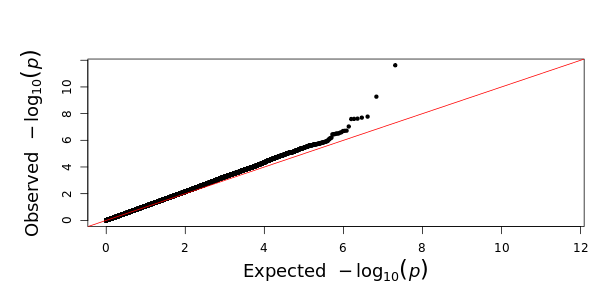
\includegraphics[width=1.0\textwidth]{Vector/ukibdgc_ibdbr_perianal_timesincediag5yrsctrl_allcase_meta_qq}

    
  \end{subfigure} 

    \begin{subfigure}[t]{1.0\textwidth}
      \centering   

      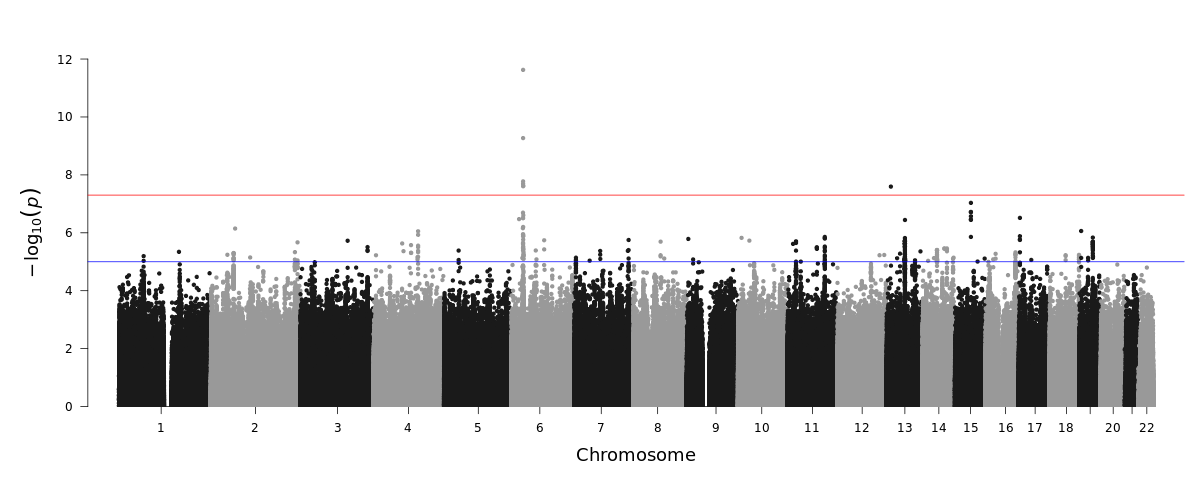
\includegraphics[width=0.8\textwidth]{Vector/ukibdgc_ibdbr_perianal_timesincediag5yrsctrl_allcase_meta}

      
  \end{subfigure} 
  \caption[Figure]{(a) Quantile-quantile plot for the meta-analysis between UKIBDGC and IBD-BR cohorts, suggesting a good fit to the uniform distribution, and showing no evidence of genomic inflation (median $\chi^{2}$=0.47; $\lambda_{GC}$=1.03; median $\chi^{2}$ was calculated by converting P-values to $\chi^{2}$  values using the function \Verb+qchisq(P, df=1,lower.tail=F)+ in R v4.1.0). (b) Manhattan plot of meta-analysis between IBD-BR and UKIBDGC. pCD+ cases are defined as CD patients with any type of perianal involvement and pCD- controls are defined as CD patients with no perianal involvement.}
  \label{fig:meta_qq_manhattan}
  \end{figure}
  % \begin{figure}[H] 
  %   \centering    
  %   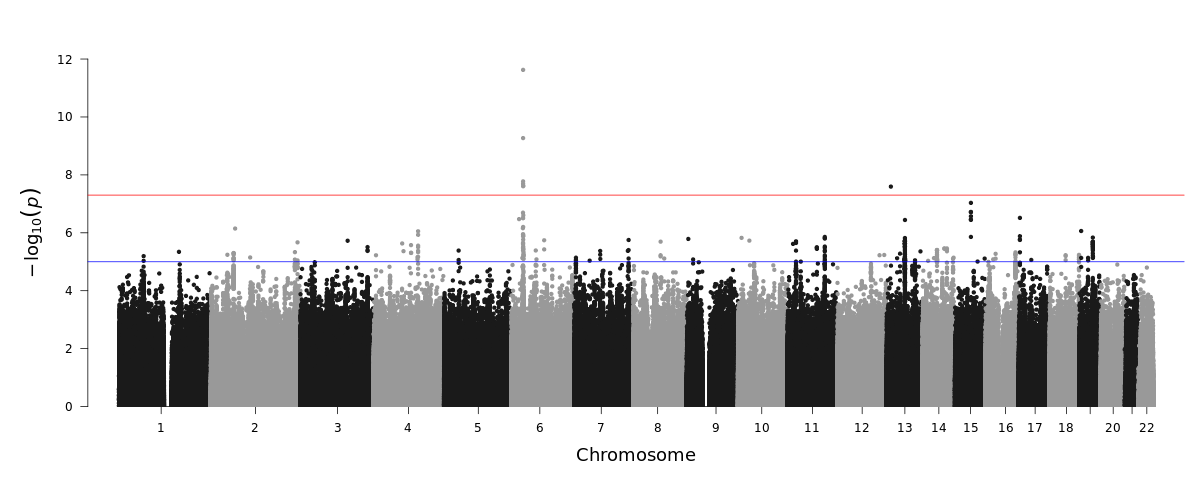
\includegraphics[width=1.0\textwidth]{Vector/ukibdgc_ibdbr_perianal_timesincediag5yrsctrl_allcase_meta}
  %   \caption[Figure]{Manhattan plot of meta-analysis between IBD-BR and UKIBDGC. pCD+ cases are defined as CD patients with any type of perianal involvement and pCD- controls are defined as CD patients with no perianal involvement.}
  %   \label{fig:meta_manhattan}
  %   \end{figure}

  


  % \subsubsection{Power analysis}
  % The ability of a GWAS study to make genome-wide significant discoveries depends on its statistical power. Statistical power is defined as the probability of correctly declaring genome-wide significance, when the alternative hypothesis that a variant is genome-wide significant it true. Statistical power analysis can therefore be used as a diagnostic test to check if the discovered variants are expected under a given study sample size its case proportion. Given a variant's MAF, effect size, a power value close to 1 indicates that the discovery is indeed expected given the study sample size. Generally, I found that the study was adequately powered to discover three of the four genome-wide significant variants (power > 0.8), and one of the variants was detectable with a power of 0.78 (Figure \ref{fig:power_analysis}). The study had an almost complete power to detect 6:32279268\_T\_G and 6:32333650\_C\_T, the two most significant variants (power > 0.98). This shows that the meta-analysis is reasonably powered to detect the genome-wide significant locus. 

  %   \begin{figure}[H] 
  %     \centering    
  %     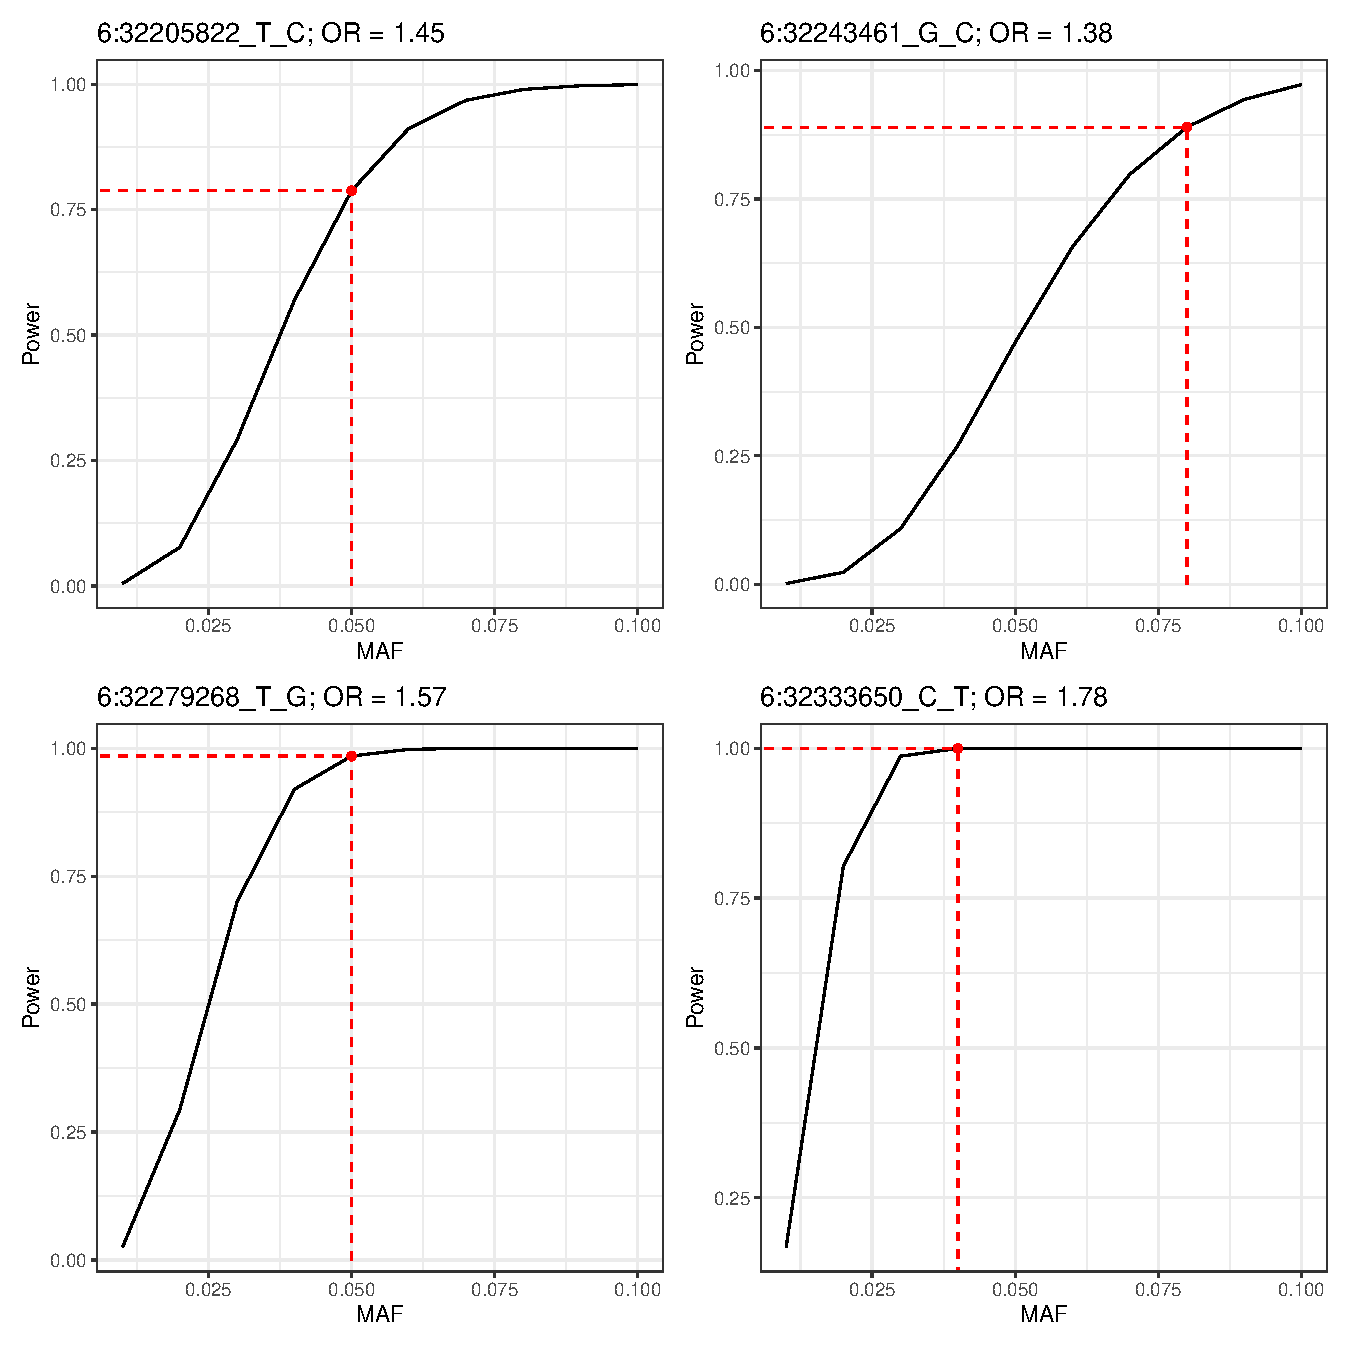
\includegraphics[width=0.7\textwidth]{power_analysis}
  %     \caption[Figure]{Power analysis for each of the genome-wide significant variants over a range of MAFs. Title, red dots and dotted lines indicate the MAF and power of the variant}
  %     \label{fig:power_analysis}
  %     \end{figure}
    
     
    \begin{figure}[H] 
      \centering    
      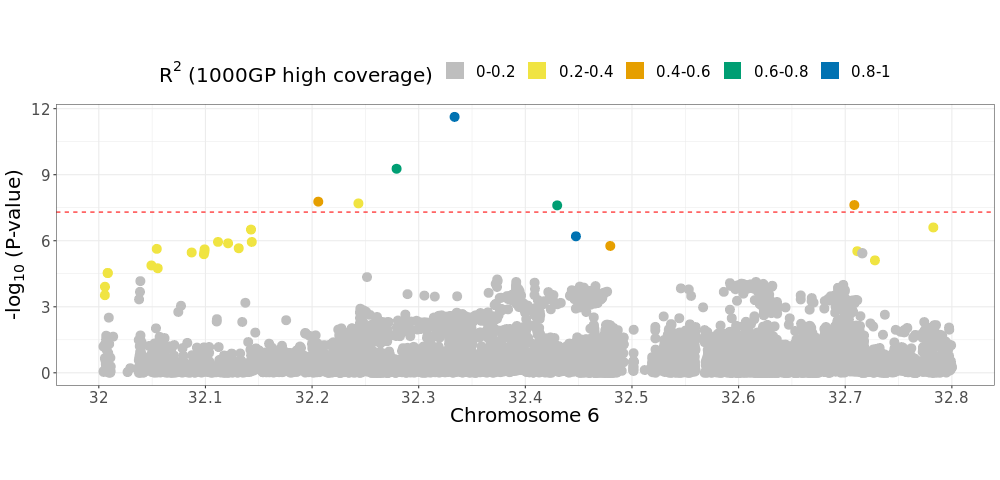
\includegraphics[width=0.8\textwidth]{Vector/regional_assoc_plot}
      \caption[Figure]{Regional association plot showing meta-analysis association P-values in 6p21.32. Variants are coloured by $R^{2}$ with the index variant, derived from 1000 Genomes Project High Coverage study (Non-Finnish Europeans)}
      \label{fig:regional_assoc_plot}
      \end{figure}
%     \subsubsection{Consistency of MAFs at 6p21.32}
   
%   The meta-analysis combined summary statistics from two different IBD cohorts genotyped using three arrays and three imputation reference panels. Given this multitude of genotyping and imputation platforms, it is conceivable that poor genotyping and/or imputation could lead to unreliable results in one of the cohorts. Additionally, cryptic population structure that is specific to one of the cohorts could also contribute to spurious associations. Checking the consistency of MAF across the cohorts can give an assurance that the genome-wide significant associations at this locus are reliable. 
  
  
%  First, I observed that all variants had consistently higher cohort than population MAFs (Table \ref{tab:table:maf_concord}). Such a systematic difference in MAF may be expected if these variants are also associated with CD risk, since the constituent cohorts are composed entirely of CD patients. In support of this, I found that two of the four variants were associated with CD in an independent UKBB-based GWAS study, explaining the higher cohort MAFs (replication P-value < 0.025).  Moreover, I compared case and control MAFs across cohorts, and found that case MAFs were systematically higher than control MAFs, which is expected given the pCD-risk-increaseing effect of the minor alleles. More importantly, case MAFs were consistent across cohorts, as were control MAFs (index variant case MAF: 0.042, 0.059, and 0.055; control MAF: 0.027, 0.037, and 0.035, in IBD-BR, UKIBGC-HCE and UKIBDGC-GWAS1 respectively).

%     \begin{table}[H]

%       \caption{\label{tab:table:maf_concord}Minor allele frequencies for the genome-wide significant variants in the 6p21.32 locus in the meta-analysis constituent cohorts, and in two population cohorts (1000 Genomes Project and GnomAD; Non-Finnish Europeans). Association P-value with Crohn's Disease are shown (obtained from the Open Targets Genetics Portal).}
%       \centering
%       \fontsize{9}{11}\selectfont
%       \begin{tabular}[t]{lrrrrrl}
%       \toprule
%       \multicolumn{1}{c}{ } & \multicolumn{2}{c}{Population Cohorts} & \multicolumn{3}{c}{Study Cohorts} & \multicolumn{1}{c}{ } \\
%       \cmidrule(l{3pt}r{3pt}){2-3} \cmidrule(l{3pt}r{3pt}){4-6}
%       SNP & 1000GP & GnomAD & IBD-BR & UKIBDGC (HCE) & UKIBDGC (GWAS1) & CD P-value\\
%       \midrule
%       6:32333650\_C\_T & 0.012 & 0.012 & 0.033 & 0.041 & 0.042 & NA\\
%       6:32279268\_T\_G & 0.015 & 0.020 & 0.044 & 0.050 & 0.050 & NA\\
%       6:32205822\_T\_C & 0.021 & 0.028 & 0.053 & 0.054 & 0.053 & $4.8\times10^{-11}$\\
%       6:32243461\_G\_C & 0.036 & 0.052 & 0.074 & 0.076 & 0.081 & $5.6\times10^{-7}$\\
%       \bottomrule
%       \end{tabular}
%       \end{table}
  

    \subsubsection{Association signal at 6p21.32 matches expected linkage disequilibrium pattern in non-Finnish Europeans}
    Although the four variants spanned a 130 kbp region, they displayed high LD with the index variant, as the 6p21 region is known to exhibit long-range LD (Figure \ref{fig:regional_assoc_plot}). To better understand if the association strength matches the expected LD pattern, I measured the correlation between the association P-value and $R^{2}$ with the index variant. The underlying assumption is that, for a given variant in a locus, the lower its LD with the index variant, the weaker its association is expected to be. P-values that do not match this expectation may suggest a spurious association due to a genotyping or imputation error or cryptic population structure. At 6p21.32, I found that LD friends P-values were correlated with the expected $R^{2}$ with the index variant ($\rho$=0.45; LD friends defined as variants with $R^{2}$ > 0.5 with the index variant and P-value < 0.01; Figure \ref{fig:ld_pval_plot}). The relatively weak correlation is likely driven by the small number of LD friends that the index variant has (N=4). When I relaxed the $R^{2}$ cutoff of LD friends this correlation became increasingly stronger ($\rho$=0.65 and 0.72 at $R^{2}$ > 0.4 and 0.2, respectively), showing that overall the variants at this locus follow their expected association strength given the LD structure between variants. 




    \begin{figure}[H] 
      \centering    
      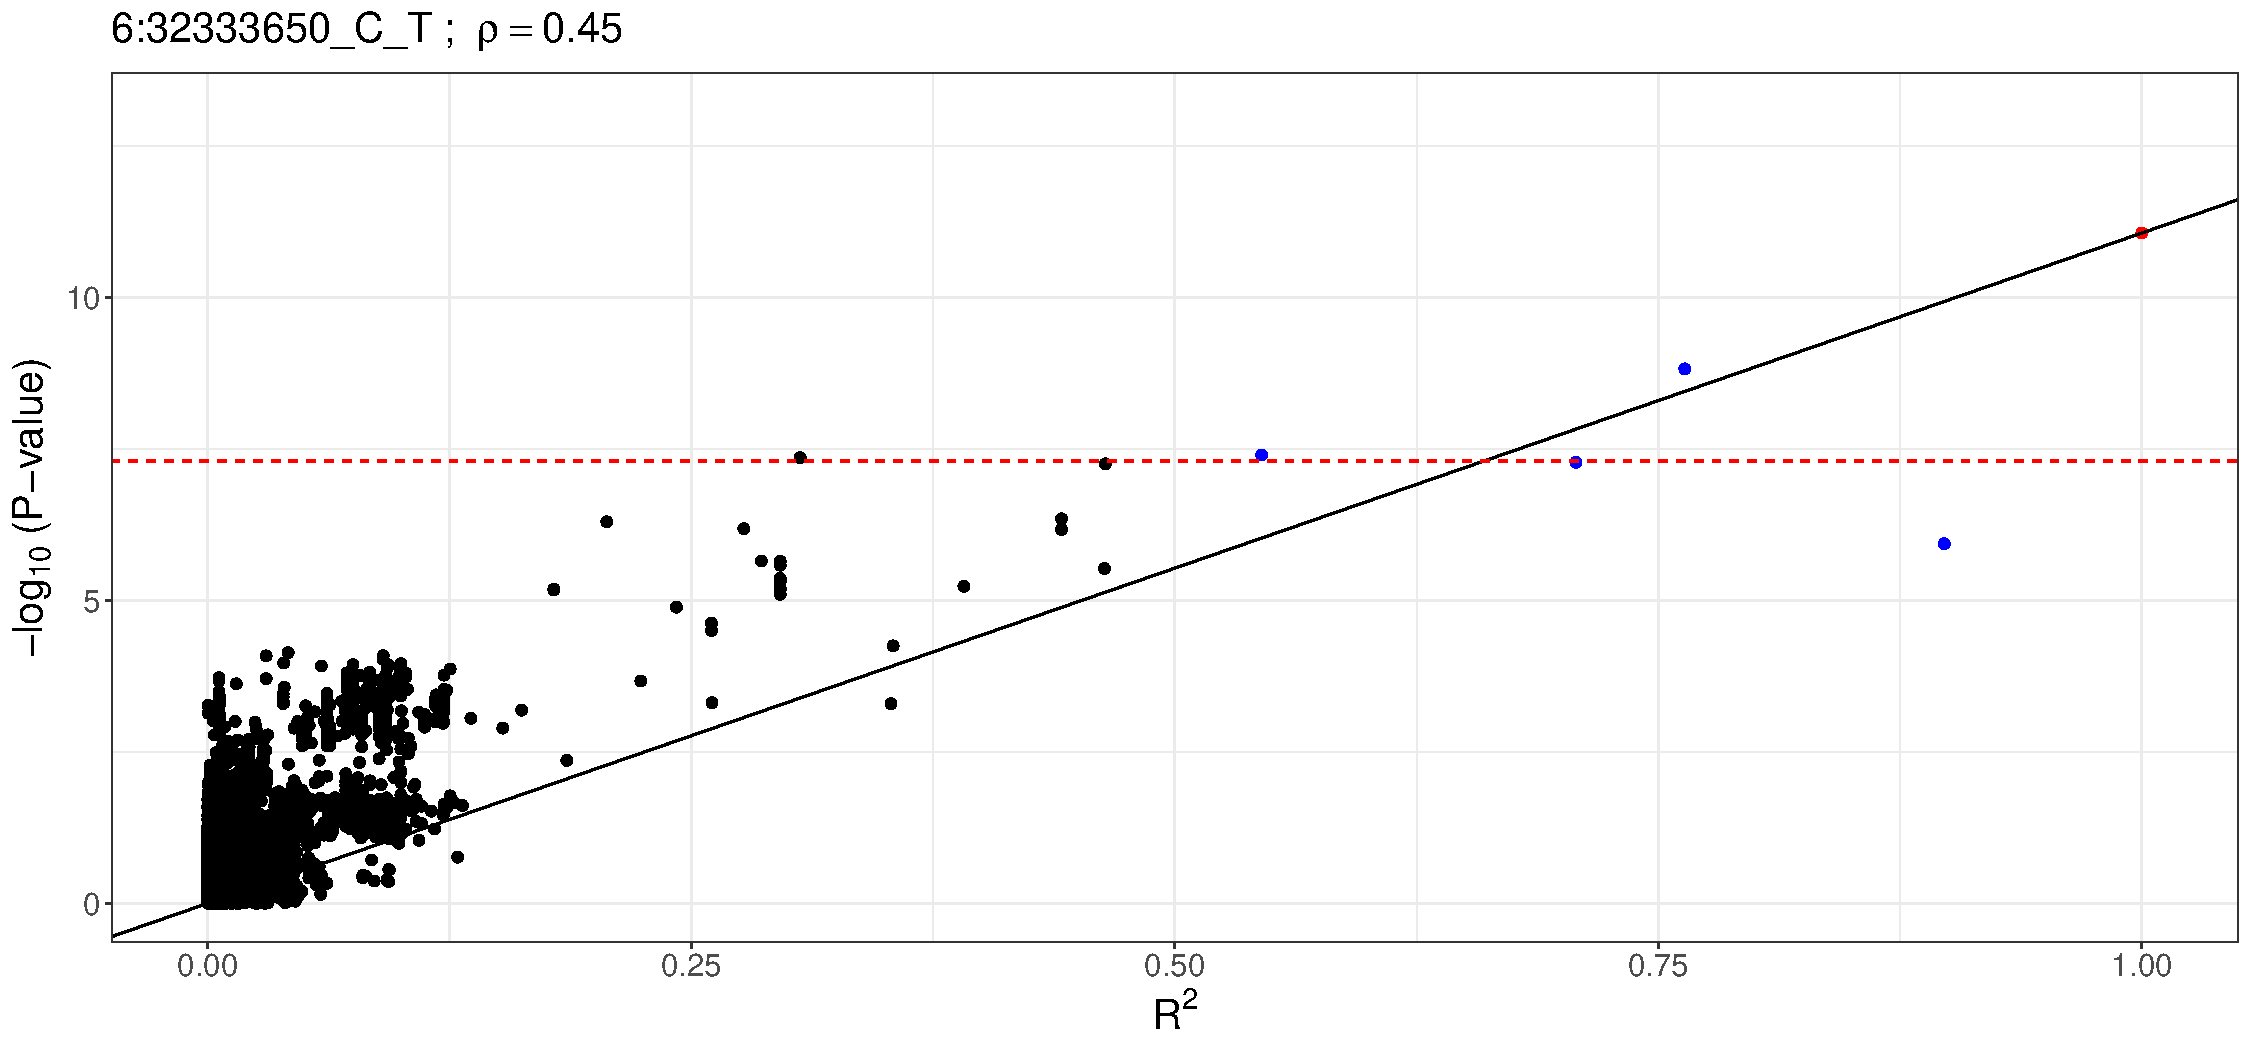
\includegraphics[width=1.0\textwidth]{fig3}
      \caption[Figure]{Association P-value for all variants in a 1mbp window around rs115378818 (P-value < $5\times10^{-4}$) on the x-axis, and $R^{2}$ of variants with the index variant on the y-axis (derived from 1000GP). Horizontal red-line indicates the genome-wide significance threshold (P-value = $5\times10^{-8}$).}
      \label{fig:ld_pval_plot}
      \end{figure}


    \subsection{Association at 6p21.32 is robust to more severe pCD+ definitions}


The IBD-BR provides information about the type of perianal involvement each patient presents with. To understand the effect of different definition criteria, I investigated how the meta-analysed association signal at 6p21.32 is sensitive to different definitions of pCD+ cases in the IBD-BR. In addition to the broad-definition meta-analysis described in the previous section ($META_{broad}$), I performed a meta-analysis between UKIBDGC and IBD-BR using three additional pCD+ definitions that have an increasingly severe impact on patients: pCD+ as abscess or simple or complex fistula only ($META_{abscfist}$), as simple or complex fistula only ($META_{fist}$), and as complex fistula only ($META_{complexfist}$). 

\begin{figure}[H] 
  \centering    
  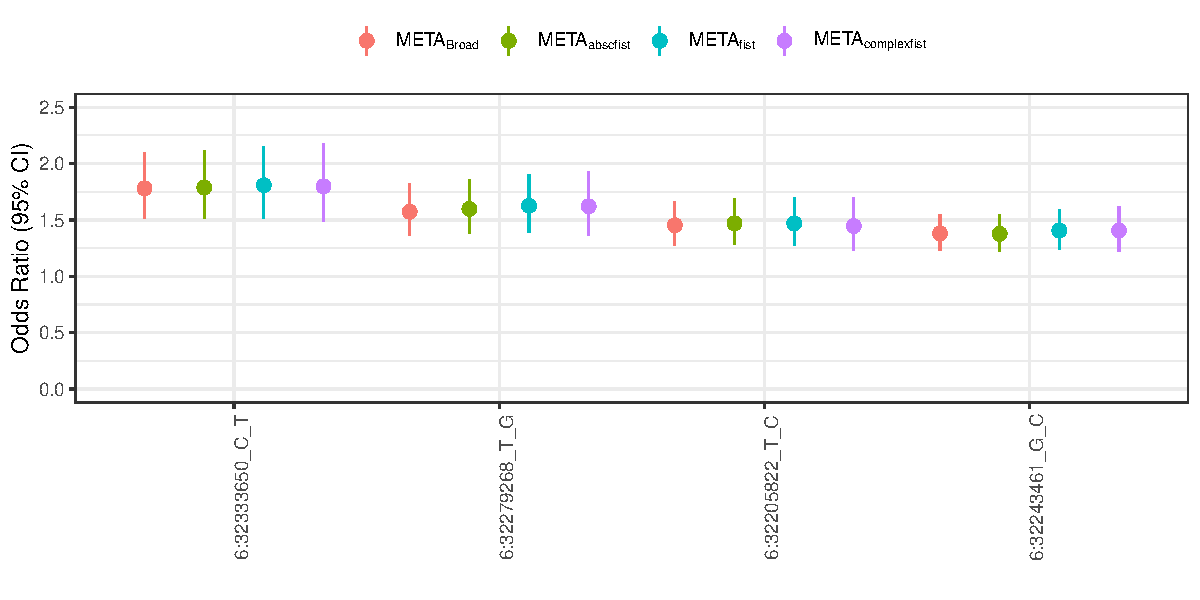
\includegraphics[width=1.0\textwidth]{pcd_def_or_plot}
  \caption[Figure]{Odds ratios of all four genome-wide significant SNPs in pCD cohorts defined with different case inclusion criteria.}
  \label{fig:pcd_def_or_plot}
  \end{figure}


I compared the effect sizes of the four-genome-wide significant SNPs and found that none of them exhibited heterogeneity of effect sizes across the different pCD definition meta-analyses ($P_{het}$ > 0.01). Additionally, I compared the association statistic between different definitions. Since the stricter definitions resulted in a reduction in the number of pCD+ cases, a proportional decrease in association test statistic ($\chi^{2}$) may also be expected. Under the hypothesis that the stricter-definition meta-analyses are simply a random subset of $META_{broad}$, the $\chi^{2}$  observed in any definition meta-analysis should match $\chi^{2}$ from $META_{broad}$ adjusted for the reduction in sample size (I will refer to this as $\chi^{2}_{Broad,n}$; see Methods for how this adjustment was performed). \\

In a 1mbp window centred around the index variant, I compared the $\chi^{2}$ statistics observed in each of the three stricter-definition meta-analyses to $\chi^{2}_{Broad,N}$. All four genome-wide significant variants achieved the expected association in the stricter definition meta-analyses. For example, rs115378818 remained genome-wide significant in $META_{fist}$ despite the decrease in sample size (1,234 fewer pCD+ cases; observed P-value=$2.2\times10^{-11}$; broad-definition P-value adjusted for sample size=$3\times10^{-11}$; Figure \ref{fig:meta_def_comparison}). More broadly, across all variants in 6p21.32, I observed strong correlation between observed $\chi^{2}$ in the stricter-definition meta-analyses and $\chi^{2}_{Broad,n}$, which shows the robustness of the association signal against different definitions of pCD+ cases in IBD-BR ($META_{abscfist}$=0.95; $META_{fist}$=0.92,$META_{complexfist}$=0.84). 

%%%%%%%%%%%%%%%%%%%%%%%%%%%%%%%%%%%%%%%%%
%FIGURE SOURCE: /lustre/scratch123/hgi/mdt2/projects/ibdgwas_ukibdgc/oe2/scripts/compare_chi_squared.R
%%%%%%%%%%%%%%%%%%%%%%%%%%%%%%%%%%%%%%%%%
\begin{figure}[H] 
  \centering    
  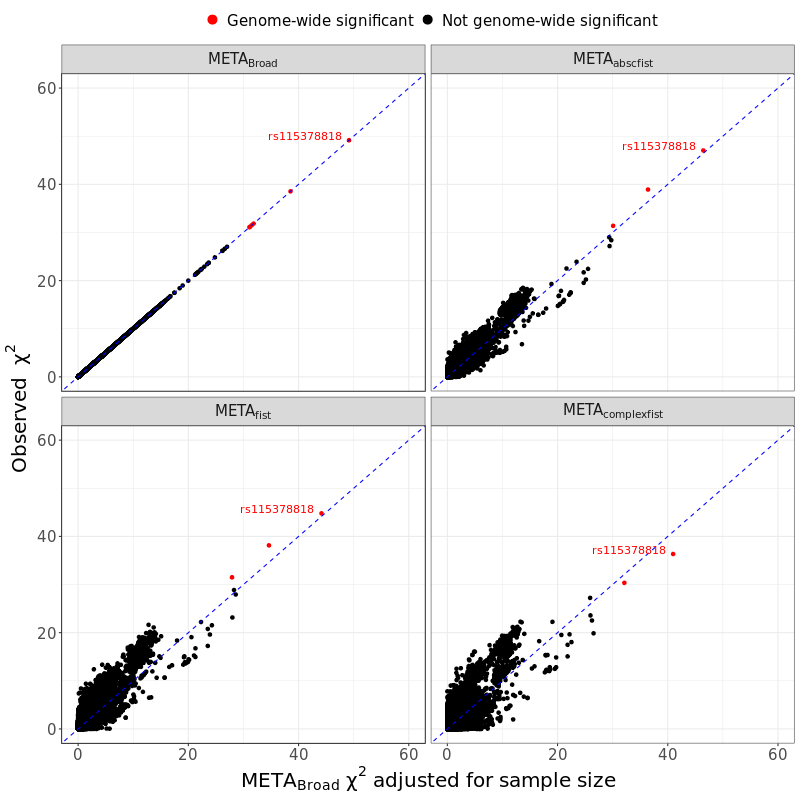
\includegraphics[width=0.8\textwidth]{Vector/meta_chisq_plot}
  \caption[Figure]{Association P-value for all variants in a 1mbp window around rs115378818 (P-value < $5\times10^{-4}$) on the x-axis, and $R^{2}$ of variants with the index variant rs115378818 on the y-axis (derived from 1000GP). The blue line indicates the line that passess through the points (0,0) and ($\chi^{2}_{Broad,n}$,$\chi^{2}_{observed}$).}
  \label{fig:meta_def_comparison}
  \end{figure}
\subsection{pCD is associated with HLA allele DRB1*01:03}
The MHC region is known to be highly polymorphic and to exhibit long-range LD patterns, which often span several hundred kbps. This makes the mapping of MHC associations to effector genes challenging \cite{Matzaraki2017-za}. To this end, HLA imputation based on genotyped variants can aid the interpretation of genome-wide significant hits in the MHC locus. HLA genes are broadly divided into class I and class II genes \cite{Marsh2010-mq}. Both classes of genes are responsible for presenting antigens to T lymphocytes and natural killer cells via antigen-presenting cells in order to initiate an innate and adaptive immune response \cite{Shiina2009-wt}. Due to the extensive polymorphism of the MHC regions, groups of HLA alleles are categorised in HLA groups which are referenced using a 2-digit naming system \cite{hla-nomenclature} (2-digit reolution; which I will refer to as \textit{allele group}). Two additional digits may be used to reference the specific HLA allele \cite{hla-nomenclature-4digit} (4-digit reolution; which I will refer to as \textit{specific allele}). 

To identify which HLA allele is associated with pCD, I performed association analyses between pCD status and class I and II HLA alleles, both at the allele group and specific allele levels (2-digit and 4-digit resolutions; see Methods for how HLA imputation was performed). Similar to the genome-wide association analysis, I performed the HLA association analyses separetely for IBD-BR and UKIBDGC and subsequently meta-analysed the summary statistics (effect sizes and standard errors). \\

None of the tested HLA alleles achieved genome-wide significance (P-value < $5\times10^{-8}$) within the cohorts or in the meta-analysis. At the allele group level, DRB1*01 had the strongest association. At a specific allele level, HLA-DRB1*01:03 had the most significant association, and had a stronger association compared to its allele group ($P_{DRB1*01:03}=1.8\times10^{-6}$; $P_{DRB1*01}=1.4\times10^{-3}$). I tested both dominant and additive modes of inheritance and found that the dominant model achieved better model fit at both the allele group and specific allele levels ($AIC_{dominant} < AIC_{additive}$; Table \ref{table:hla_allele_assoc}). 
\begin{table}[H]
  
  \centering\begingroup\fontsize{9}{10}\selectfont
  \caption{Top HLA allele associations with pCD status. Both allele groups (2-digit resolution; first two rows) and specific alleles (4-digit resolution; third and fourth rows) are shown. Meta-analysed P-values and odds ratios between UKIBDGC and IBD-BR cohorts are shown (with their 95\% confidence intervals). Both dominant and additive modes of inheritance  for  DRB1*01 and DRB1*01:03 were tested. Akaike Information Content (AIC), a measure of model fit, is shown in the last theree columns for each of the three constituent cohorts, and shows a better fit for the dominant model (lower AIC).}
  \label{table:hla_allele_assoc}
  \begin{tabular}[t]{|l|l|l|l|l|l|l|}
  \hline
  HLA Allele & Inheritance & Odds Ratio & P-value & AIC (IBDBR) & AIC (HCE) & AIC (GWAS1)\\
  \hline
  DRB1*01 & Dominant & 1.2 (1.1 - 1.3) & 9.4e-04 & 9127.887 & 3901.092 & 1783.907\\
  \hline
  DRB1*01 & Additive & 1.1 (1.1 - 1.2) & 1.5e-03 & 9128.485 & 3901.413 & 1783.907\\
  \hline
  DRB1*01:03 & Dominant & 1.6 (1.3 - 1.9) & 5.3e-07 & 9122.007 & 3651.987 & 1615.647\\
\hline
DRB1*01:03 & Additive & 1.5 (1.3 - 1.8) & 1.8e-06 & 9122.825 & 3653.500 & 1615.647\\
\hline
  \end{tabular}
  \endgroup{}
  \end{table}
\subsubsection{Conditioning association signal on DRB1*01:03}
I then asked if the DRB1*01:03 association with pCD accounted for the genome-wide significant locus at 6p21.32. Linking the two associations can explain which HLA allele the genome-wide significant hit may map to. To this end, I repeated the association tests for all variants in the locus, including DR1*01:03 as a covariate. Additionally, I repeated the HLA allele association test conditioning on the index variant in the locus to understand if the DRB*01:03 association is completely accounted for by the index variant. Similar to the GWAS and the HLA allele association tests, I also analysed the different cohorts separately and then meta-analysed the effect sizes and standard errors.\\


After conditioning on the index variant rs115378818, I did not observe an association with DRB1*01:03, indicating that the  DRB1*01:03 association is completely accounted for by the index variant ($P_{DRB1*01:03|rs115378818}$=0.61). Conversely, DRB1*01:03 did not completely account for the rs115378818 association. When I conditioned the rs115378818 association on DRB1*01:03, the index variant remained nominally associated with pCD ($P_{rs115378818}=8.6\times10^{-12}$ and  $P_{rs115378818|DRB1*01:03}=1.1\times10^{-5}$; Figure \ref{fig:residual_assoc_plot}). Taken together, this evidence suggests that  DRB1*01:03 is only nominally associated with pCD and that it only partly explains the observed genome-wide association signal. 

 
\begin{figure}[H] 
  \centering    
  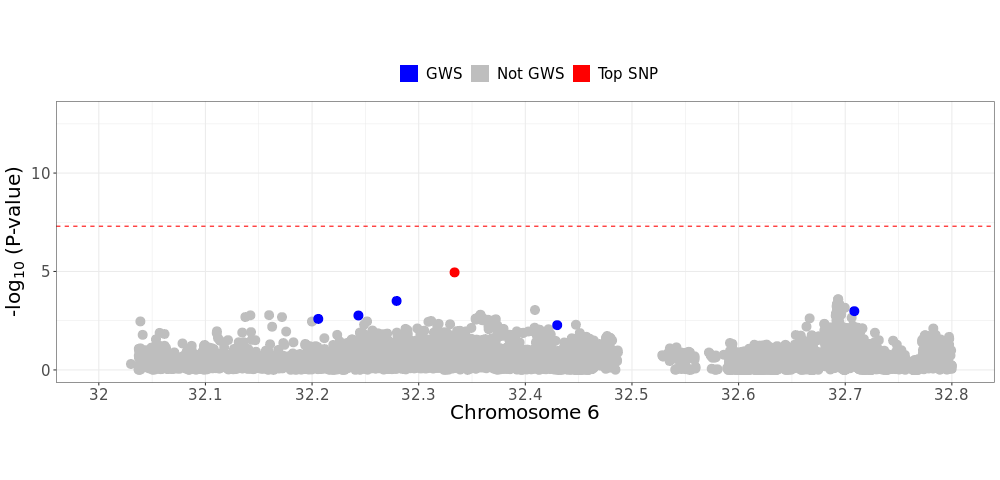
\includegraphics[width=0.7\textwidth]{Vector/cond_regional_assoc_plot}
  \caption[Figure]{Residual association signal after including DRB1*01:03 as a covariate. Blue points represent variants with a genome-wide significant association in the model that does not include DRB1:01*03. The red point indicates rs115378818 (index variant).}
  \label{fig:residual_assoc_plot}
  \end{figure}

  
\section{Discussion}
In this chapter, I have used two IBD cohorts (UKIBDGC and IBD-BR) with rich clinical data to describe the clinical characteristics of pCD and identify genetic variants associated with pCD risk. With a total of 12,897 individuals, this meta-analysis represents one of the largest pCD GWAS studies to date \cite{Akhlaghpour2023-jw}. Although others have attempted to identify pCD-associated loci, none of the studies have found genome-wide significant hits \cite{Akhlaghpour2023-jw,Kaur2016-ut}. The most recent pCD study by Akhlaghpour et al. identified a Complement Factor B (\textit{CFB}) missense variant that was nominally associated with pCD risk (rs4151651; P-value=$9.35\times10^{-6}$). \textit{CFB} is part of the alternative pathway responsible for the activation of the complement system, an innate immune subsystem that improves the ability of phagocytic cells to clear pathogens \cite{Huang2002-of,Goring2009-cs}. Functional follow-up work showed that the \textit{CFB} missense variant impairs the phagocytic ability of macrophages. This impaired phagocytic capability was hypothesised to impact the ability of the immune system to fight bacterial strains found in the fistulas of CD patients. Although this study established a plausible factor that may contribute to pCD risk, a more complete picture of its pathogenesis is needed.\\


In an attempt to fill the gap in our understanding of pCD pathogenesis, I performed a meta-analysis of two pCD cohorts, with a total of 3,967 pCD+ cases and 8,930 pCD- controls. I identified a genome-wide significant locus in the highly polymorphic Major Histocompatibility Locus (MHC) at 6p21.32 that was associated with pCD risk (index variant rs115378818). Additionally, my post-GWAS checks have reasonably confirmed the veracity of this association. Furthermore, the assocaition signal revealed by our meta-analysis is likely distinct from the \textit{CFB} association. First, rs115378818 and rs4151651 are in weak LD ($R^{2}$=0.24). Second, upon conditioning on the \textit{CFB} signal (rs114969413; $R^{2}$ with index variant $=0.99$), rs115378818 remained nominally associated suggesting that the \textit{CFB} does not completely account for it ($P_{rs115378818|rs114969413}$=$2.1\times10^{-6}$; Figure \ref{fig:cond_mcgovern}), and showing that our genome-wide significant variant represents a novel pCD-associated locus. \\

\begin{figure}
  \centering    
  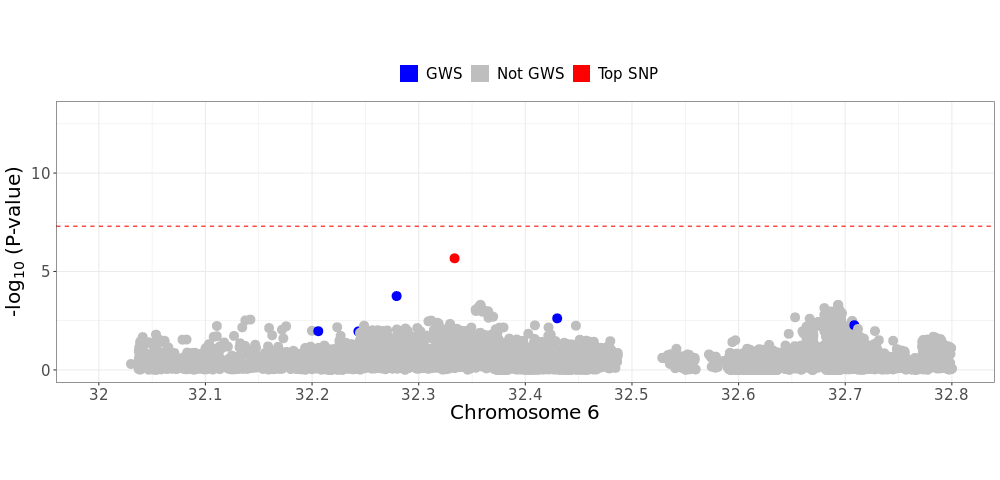
\includegraphics[width=0.7\textwidth]{Vector/cond_mcgovern_regional_assoc_plot}
  \caption[Figure]{Residual association signal after including  rs114969413 (a \textit{CFB} locus variant) as a covariate. Blue points represent variants with a genome-wide significant association in the model that does not include rs114969413. The red point indicates rs115378818 (index variant).}
  \label{fig:cond_mcgovern}
  \end{figure}
  
  Despite our ability to identify a novel association, case heterogeneity remains an important limitation of this study. Akhlaghpour et al. have also noted that a potentially heterogeneous composition of their cohorts may have decreased their power to detect genome-wide associations with pCD. Their cohorts, similar to ours, may have had patients with milder forms of pCD such as skin tags and ulcer. Therefore, I tested the association of our locus with pCD+ cases redefined with increasingly severe criteria and found that the genome-wide significant association was robust to different case definitions. However, the heterogeneity of case definition may still have decreased our power to detect \textit{additional} pCD-associated loci. In this study, a more refined definition of pCD+ as fistulising pCD was hampered by the unavailability of more granular data on the specific pCD manifestations in the UKIBDGC cohort. It remains to be seen if larger sample sizes can overcome the heterogeneity in case definition and identify more pCD-associated loci. Increasing power will not only identify more pCD-associated loci, but it will also give us a more complete understanding of the pathogenesis of pCD, and may implicate biological pathways that are targeted by pCD-associated genetic variation. \\


  Nonetheless, the finding that HLA-DRB1*01:03 may explain the genome-wide association signal is a promising starting point. HLA-DRB1*01:03 has been previously shown to be associated with colonic Crohn's disease, ulcerative colitis risk \cite{Goyette2015-xx,Cleynen2016-ha} and rheumatoid arthritis (RA) \cite{Klimenta2019-be}. However, several avenues should be explored to identify which HLA alleles completely account for the genome-wide significant association. Several reasons may explain the incomplete association of HLA-DRB*1:03 with pCD. First, the association signal at 6p21.32 may be explained by multiple HLA alleles, and therefore conditioning on a single HLA allele cannot completely explain the 6p21.32 signal. The highly polymorphic nature of most HLA genes often makes it difficult to completely attribute disease risk to a single HLA allele. This has been previously observed for rheumatoid arthritis (RA), where several \textit{HLA-DRB1} alleles confer risk to RA \cite{Van_Drongelen2017-dh}. Second, multiple \textit{HLA-DRB1} alleles with slight differences in their amino acid sequences, especially in the peptide binding regions, have different affinities to antigens being presented to T-cells \cite{Wang2022-hk}. Therefore, testing the pCD association with multiple HLA-DRB1 alleles that share the same amino acid sequences might better account for the pCD signal \cite{Molineros2019-mu}. Interestingly, Raychaudhuri et al. found that only three amino acid positions in a predictive model of RA risk provided identical prediction to a model that included all \textit{HLA-DRB1} allleles \cite{Raychaudhuri2012-em}. Therefore, an important follow-up to my work should explore the association of HLA-DRB1 alleles with pCD at the amino acid level. \\

Finally, it is important that future studies do not consider pCD as an isolated disease. The broad clinical phenotyping of IBD-BR showed lower drug intake, higher prevalence of extraintestinal manifestations, and higher prevalence of rectal CD in pCD+ patients. These observations naturally pose a question about how these disease characteristics relate to pCD. A plausible explanation is that these clinical characteristics are simply manifestations of what is collectively termed "severe CD". It is still important however to understand how severe CD drives these seemingly unrelated manifestations. For example, is there common pathogenesis, or genetic predisposition that drives all these manifestations, including pCD? In this regard, my univariate pCD meta-analysis is limited. Future studies should quantify the genetic correlation between pCD and disease severity and location, extraintestinal manifestations, and drug response. Furthermore, multivariate GWAS methods should be employed to identify shared and distinct genetic factors driving each of these manifesations. The observation that clusters of disorders have common as well as distinct genetic factors has been previously shown to further our understanding of multiple groups of disorders such as psychiatric disorders \cite{Grotzinger2019-bt}. \\





Literature about pCD pathogenesis largely attributes the development of fistlising CD to the theory of epithelial-to-mesenchymal transformation of epithelial cells. With the ongoing growth of IBD-BR, and with more genotyped CD participants, a more nuanced understanding of which dysregulated pathways give rise to pCD risk, and whether or not these pathways corroborate the EMT theory of pCD pathogenesis is increasingly attainable.


% \section{Second section of the third chapter}
% and here I write more \dots

% \section{The layout of formal tables}
% This section has been modified from ``Publication quality tables in \LaTeX*''
%  by Simon Fear.

% The layout of a table has been established over centuries of experience and 
% should only be altered in extraordinary circumstances. 

% When formatting a table, remember two simple guidelines at all times:

% \begin{enumerate}
%   \item Never, ever use vertical rules (lines).
%   \item Never use double rules.
% \end{enumerate}

% These guidelines may seem extreme but I have
% never found a good argument in favour of breaking them. For
% example, if you feel that the information in the left half of
% a table is so different from that on the right that it needs
% to be separated by a vertical line, then you should use two
% tables instead. Not everyone follows the second guideline:

% There are three further guidelines worth mentioning here as they
% are generally not known outside the circle of professional
% typesetters and subeditors:

% \begin{enumerate}\setcounter{enumi}{2}
%   \item Put the units in the column heading (not in the body of
%           the table).
%   \item Always precede a decimal point by a digit; thus 0.1
%       {\em not} just .1.
%   \item Do not use `ditto' signs or any other such convention to
%       repeat a previous value. In many circumstances a blank
%       will serve just as well. If it won't, then repeat the value.
% \end{enumerate}

% A frequently seen mistake is to use `\textbackslash begin\{center\}' \dots `\textbackslash end\{center\}' inside a figure or table environment. This center environment can cause additional vertical space. If you want to avoid that just use `\textbackslash centering'


% % %!TEX root = ../thesis.tex
%*******************************************************************************
%****************************** Third Chapter **********************************
%*******************************************************************************
\chapter{My fifth chapter}

% **************************** Define Graphics Path **************************
\ifpdf
    \graphicspath{{Chapter3/Figs/Raster/}{Chapter3/Figs/PDF/}{Chapter3/Figs/}}
\else
    \graphicspath{{Chapter3/Figs/Vector/}{Chapter3/Figs/}}
\fi

\section{First section of the third chapter}
And now I begin my third chapter here \dots

And now to cite some more people~\citet{Rea85,Ancey1996}

\subsection{First subsection in the first section}
\dots and some more 

\subsection{Second subsection in the first section}
\dots and some more \dots

\subsubsection{First subsub section in the second subsection}
\dots and some more in the first subsub section otherwise it all looks the same
doesn't it? well we can add some text to it \dots

\subsection{Third subsection in the first section}
\dots and some more \dots

\subsubsection{First subsub section in the third subsection}
\dots and some more in the first subsub section otherwise it all looks the same
doesn't it? well we can add some text to it and some more and some more and
some more and some more and some more and some more and some more \dots

\subsubsection{Second subsub section in the third subsection}
\dots and some more in the first subsub section otherwise it all looks the same
doesn't it? well we can add some text to it \dots

\section{Second section of the third chapter}
and here I write more \dots

\section{The layout of formal tables}
This section has been modified from ``Publication quality tables in \LaTeX*''
 by Simon Fear.

The layout of a table has been established over centuries of experience and 
should only be altered in extraordinary circumstances. 

When formatting a table, remember two simple guidelines at all times:

\begin{enumerate}
  \item Never, ever use vertical rules (lines).
  \item Never use double rules.
\end{enumerate}

These guidelines may seem extreme but I have
never found a good argument in favour of breaking them. For
example, if you feel that the information in the left half of
a table is so different from that on the right that it needs
to be separated by a vertical line, then you should use two
tables instead. Not everyone follows the second guideline:

There are three further guidelines worth mentioning here as they
are generally not known outside the circle of professional
typesetters and subeditors:

\begin{enumerate}\setcounter{enumi}{2}
  \item Put the units in the column heading (not in the body of
          the table).
  \item Always precede a decimal point by a digit; thus 0.1
      {\em not} just .1.
  \item Do not use `ditto' signs or any other such convention to
      repeat a previous value. In many circumstances a blank
      will serve just as well. If it won't, then repeat the value.
\end{enumerate}

A frequently seen mistake is to use `\textbackslash begin\{center\}' \dots `\textbackslash end\{center\}' inside a figure or table environment. This center environment can cause additional vertical space. If you want to avoid that just use `\textbackslash centering'








%\include{Chapter6/chapter6}
%\include{Chapter7/chapter7}



% ********************************** Back Matter *******************************
% Backmatter should be commented out, if you are using appendices after References
%\backmatter

% ********************************** Bibliography ******************************
\begin{spacing}{0.9}

% To use the conventional natbib style referencing
% Bibliography style previews: http://nodonn.tipido.net/bibstyle.php
% Reference styles: http://sites.stat.psu.edu/~surajit/present/bib.htm

% \bibliographystyle{apalike}
\bibliographystyle{unsrt} % Use for unsorted references  
%\bibliographystyle{plainnat} % use this to have URLs listed in References
\cleardoublepage
\bibliography{References/references} % Path to your References.bib file


% If you would like to use BibLaTeX for your references, pass `custombib' as
% an option in the document class. The location of 'reference.bib' should be
% specified in the preamble.tex file in the custombib section.
% Comment out the lines related to natbib above and uncomment the following line.

%\printbibliography[heading=bibintoc, title={References}]


\end{spacing}

% ********************************** Appendices ********************************

\begin{appendices} % Using appendices environment for more functunality

% %!TEX root = ../thesis.tex
% ******************************* Thesis Appendix A ****************************
\chapter{How to install \LaTeX} 


% %!TEX root = ../thesis.tex
% ******************************* Thesis Appendix B ********************************

\chapter{}


\end{appendices}

% *************************************** Index ********************************
\printthesisindex % If index is present

\end{document}
